%!TEX program = xelatex
\documentclass[cn,hazy,pku,12pt,normal,math=newtx,cite=super]{elegantnote}
\usepackage{tikz}
\usepackage{tikz}

\AddToHook{shipout/foreground}{
  \begin{tikzpicture}[remember picture,overlay]
    \node[black,rotate=0,scale=10,opacity=0.1] at ([yshift=8cm]current page.center) {Z.C. Wang};
    \node[black,rotate=0,scale=10,opacity=0.1] at ([yshift=4cm]current page.center) {Z.C. Wang}; 
    \node[black,rotate=0,scale=10,opacity=0.1] at (current page.center) {Z.C. Wang}; 
    \node[black,rotate=0,scale=10,opacity=0.1] at ([yshift=-4cm]current page.center) {Z.C. Wang};
    \node[black,rotate=0,scale=10,opacity=0.1] at ([yshift=-8cm]current page.center) {Z.C. Wang}; 
  \end{tikzpicture}
}



\title{实验二\quad 溶解热的测定\\
\Large{测量硝酸钾的溶剂过程中的热效应}}

\author{王子宸\quad 210001873\\
周四19组\quad 8号}
\institute{化学与分子工程学院}

\expdate{\zhdate{2023/9/28}}
\temperature{24.0 \si{^{\circ}C}}
\pressure{100.81 \si{kPa}}

\usepackage{array,longtable,subcaption,chngcntr}
\usepackage[version=4]{mhchem}

\pagecolor{white}
\begin{document}

\maketitle

\keywords{国家精品课 \quad 物理化学实验 \quad 硝酸钾溶解热 \quad 电热补偿法 \quad 雷诺图解法}

\abstracts{
本实验中,利用电热补偿法测定了\ce{KNO_3}在不同浓度时的水溶液中的溶解热,通过平台期校正与雷诺校正两种方法,对于测定的温度予以校正。绘制$\Delta T-t$图并拟合$Q_{\mathrm{s}}^{-1}-n_0^{-1}$的双倒数线性关系。通过经验式,计算得到$Q_{\mathrm{s}}^0 = (4.70 \pm 0.02 )\times 10^{4}\mathrm{~J\cdot mol^{-1}}$,并且进一步计算了溶解过程中的其他热效应的数值。
}

\newpage


\section{引言}

\subsection{实验目的}

\begin{figure}[htbp]
    \centering
    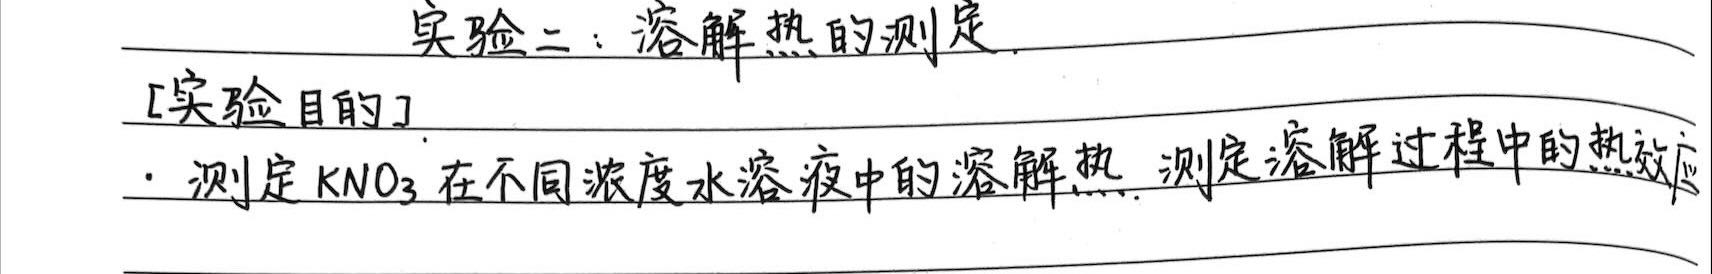
\includegraphics[width=0.9\textwidth]{figures/0-1.jpg}
    \caption{实验目的}
\end{figure}
\subsection{实验原理}
\begin{figure}[htbp]
    \centering
    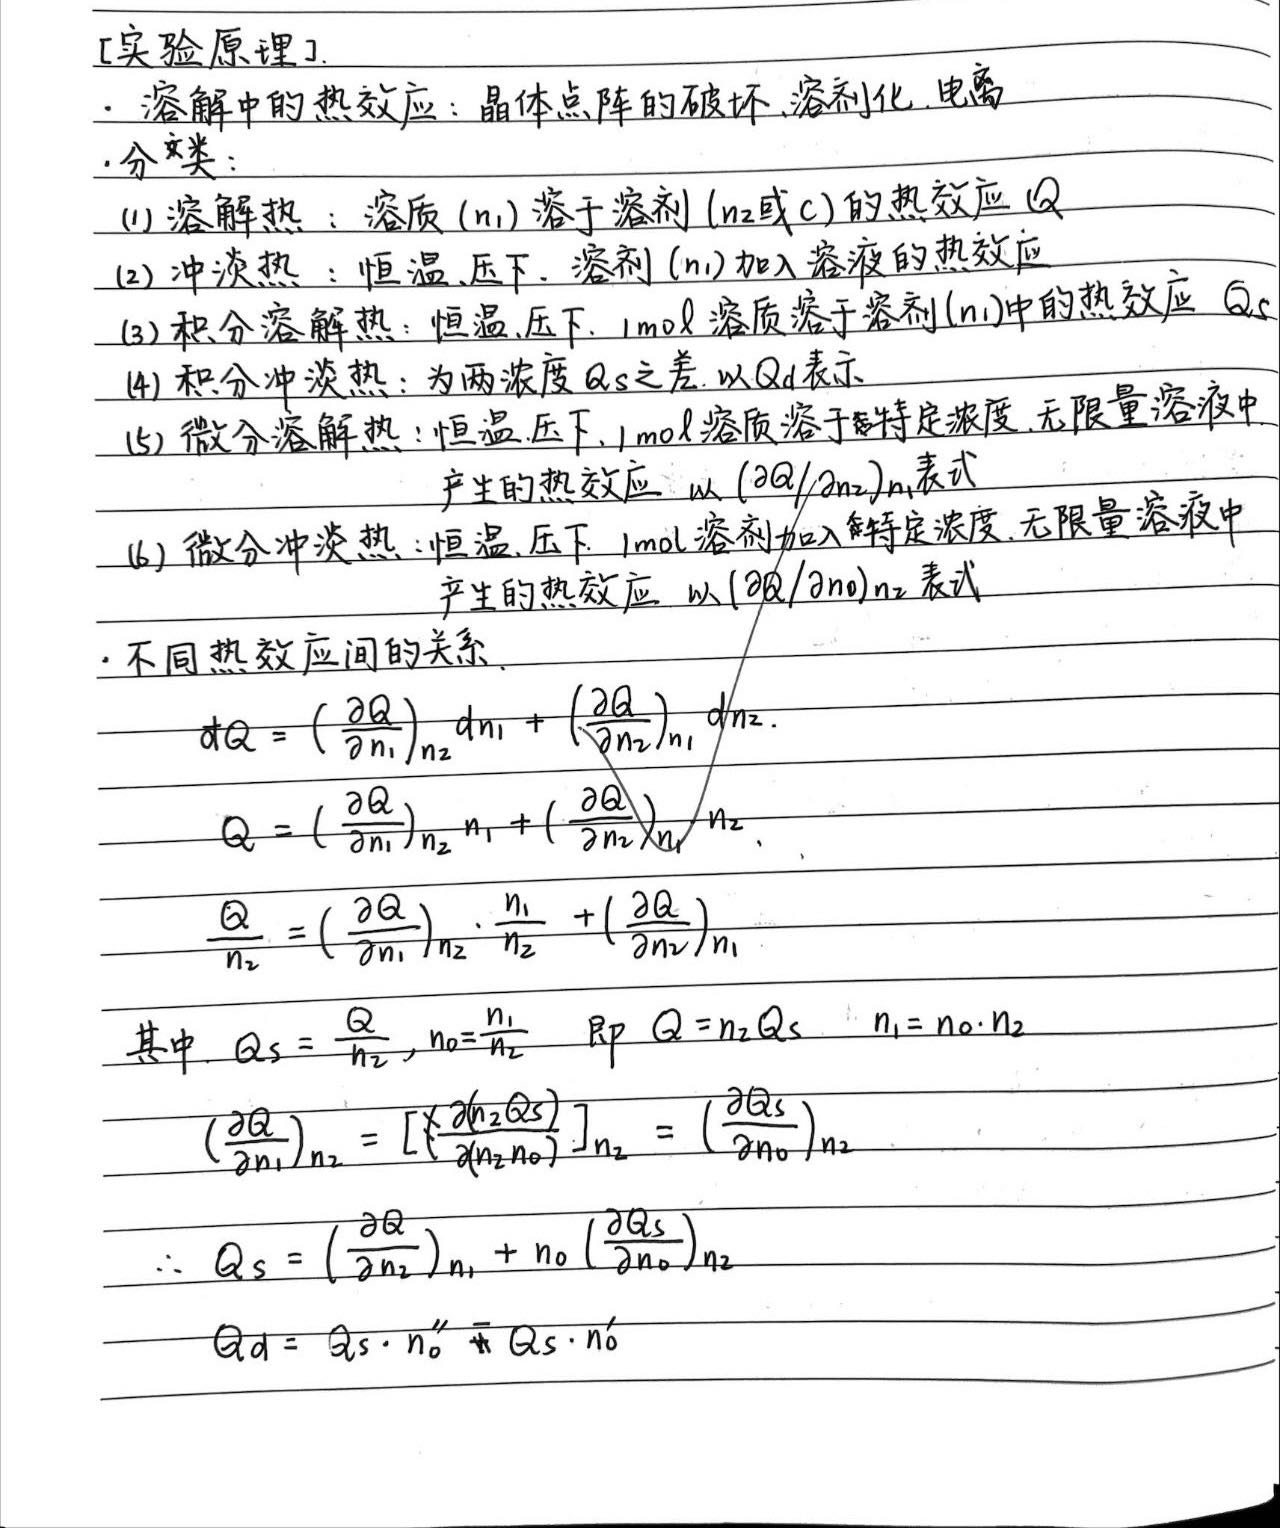
\includegraphics[width=0.75\textwidth]{figures/0-2.jpg}
    %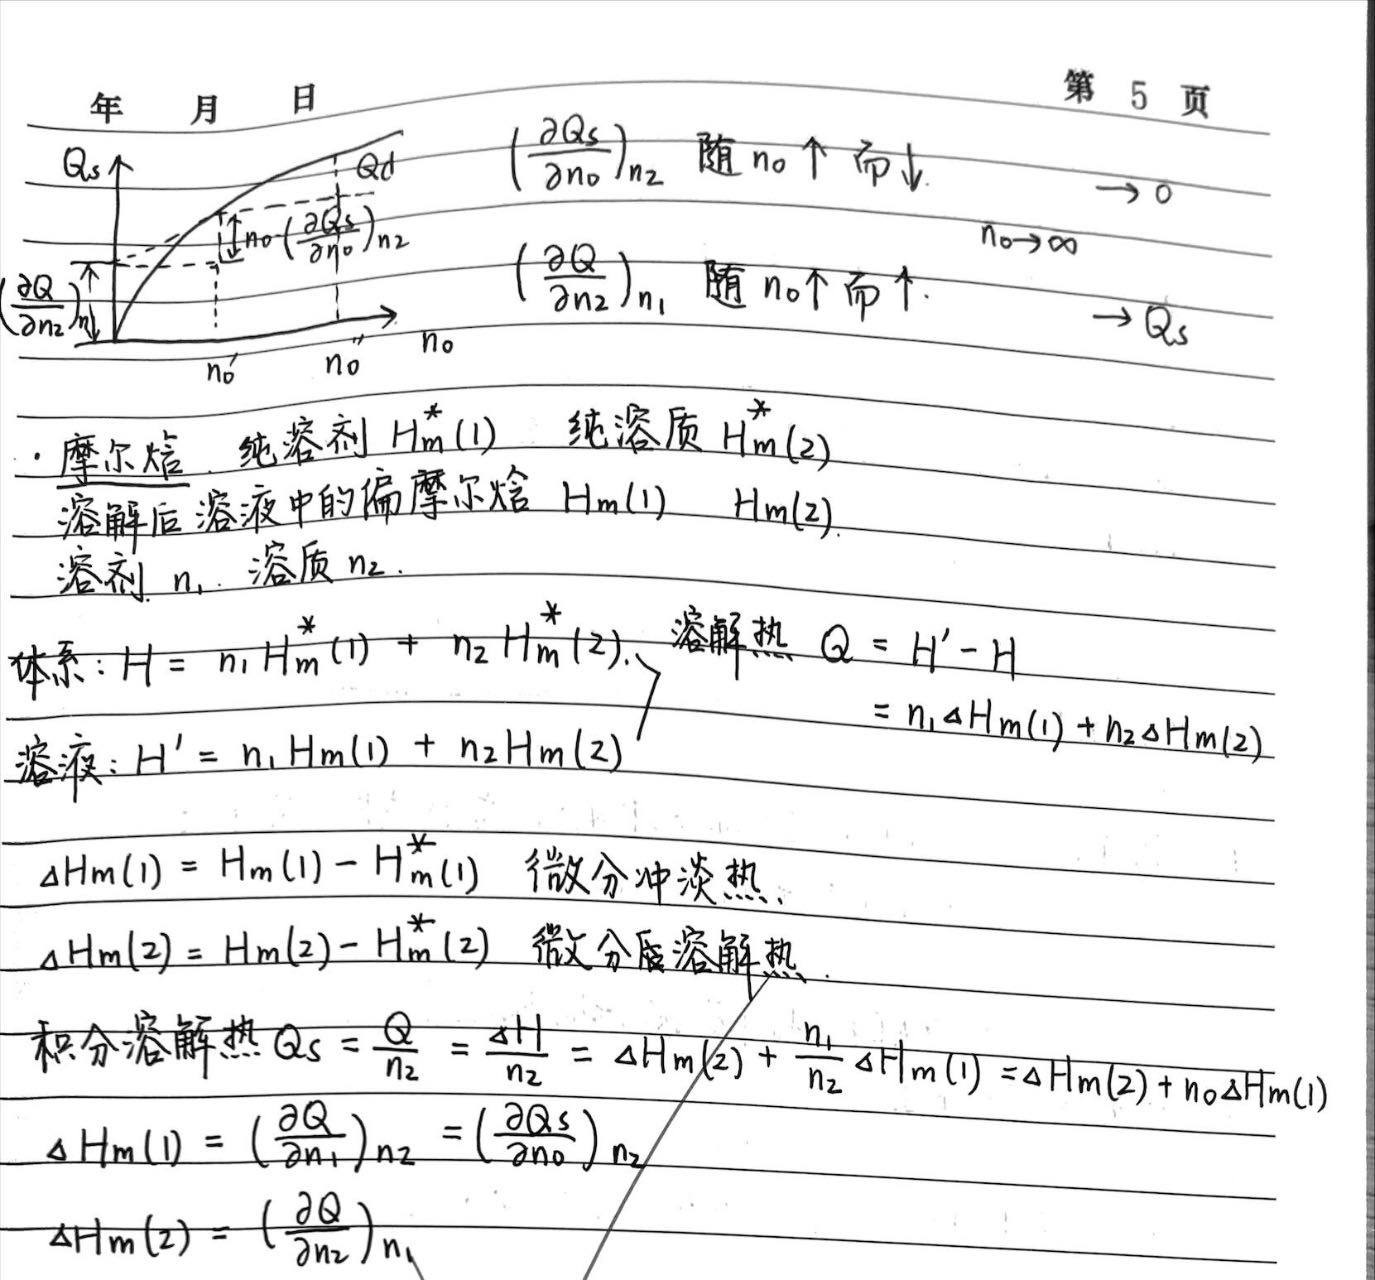
\includegraphics[width=0.75\textwidth]{figures/0-3.jpg}
    %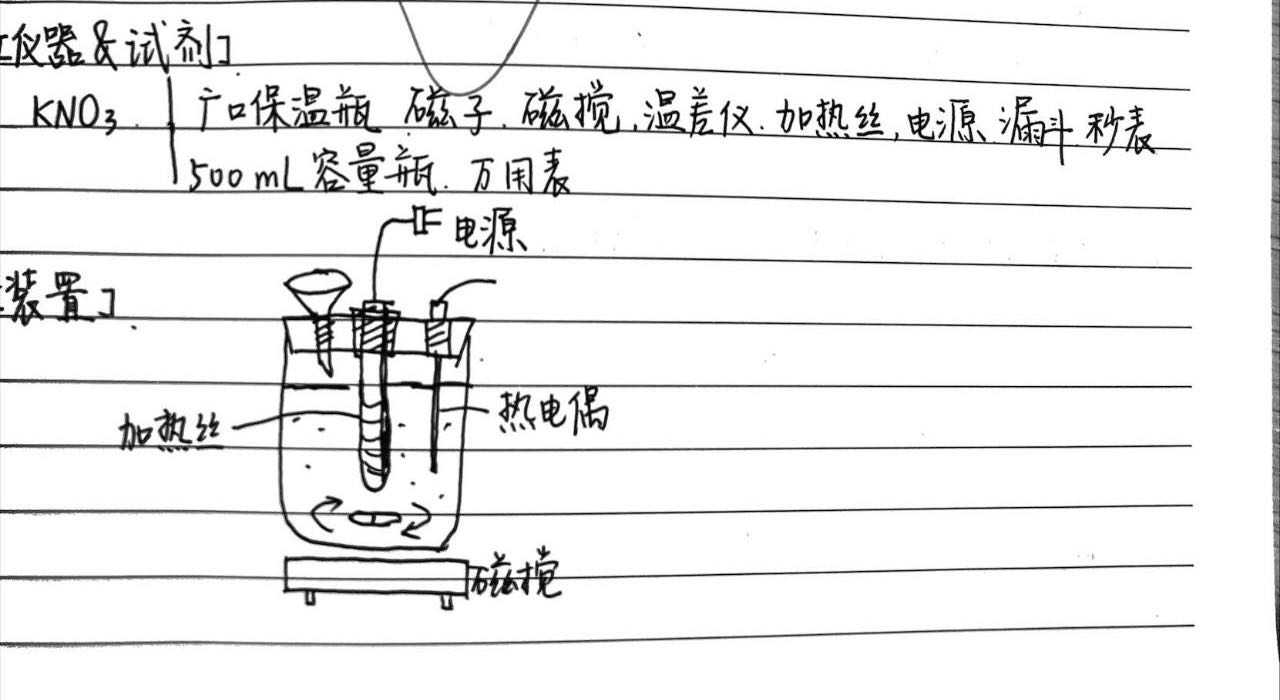
\includegraphics[width=0.75\textwidth]{figures/0-5.jpg}
\end{figure}
\begin{figure}[htbp]
    \centering
    %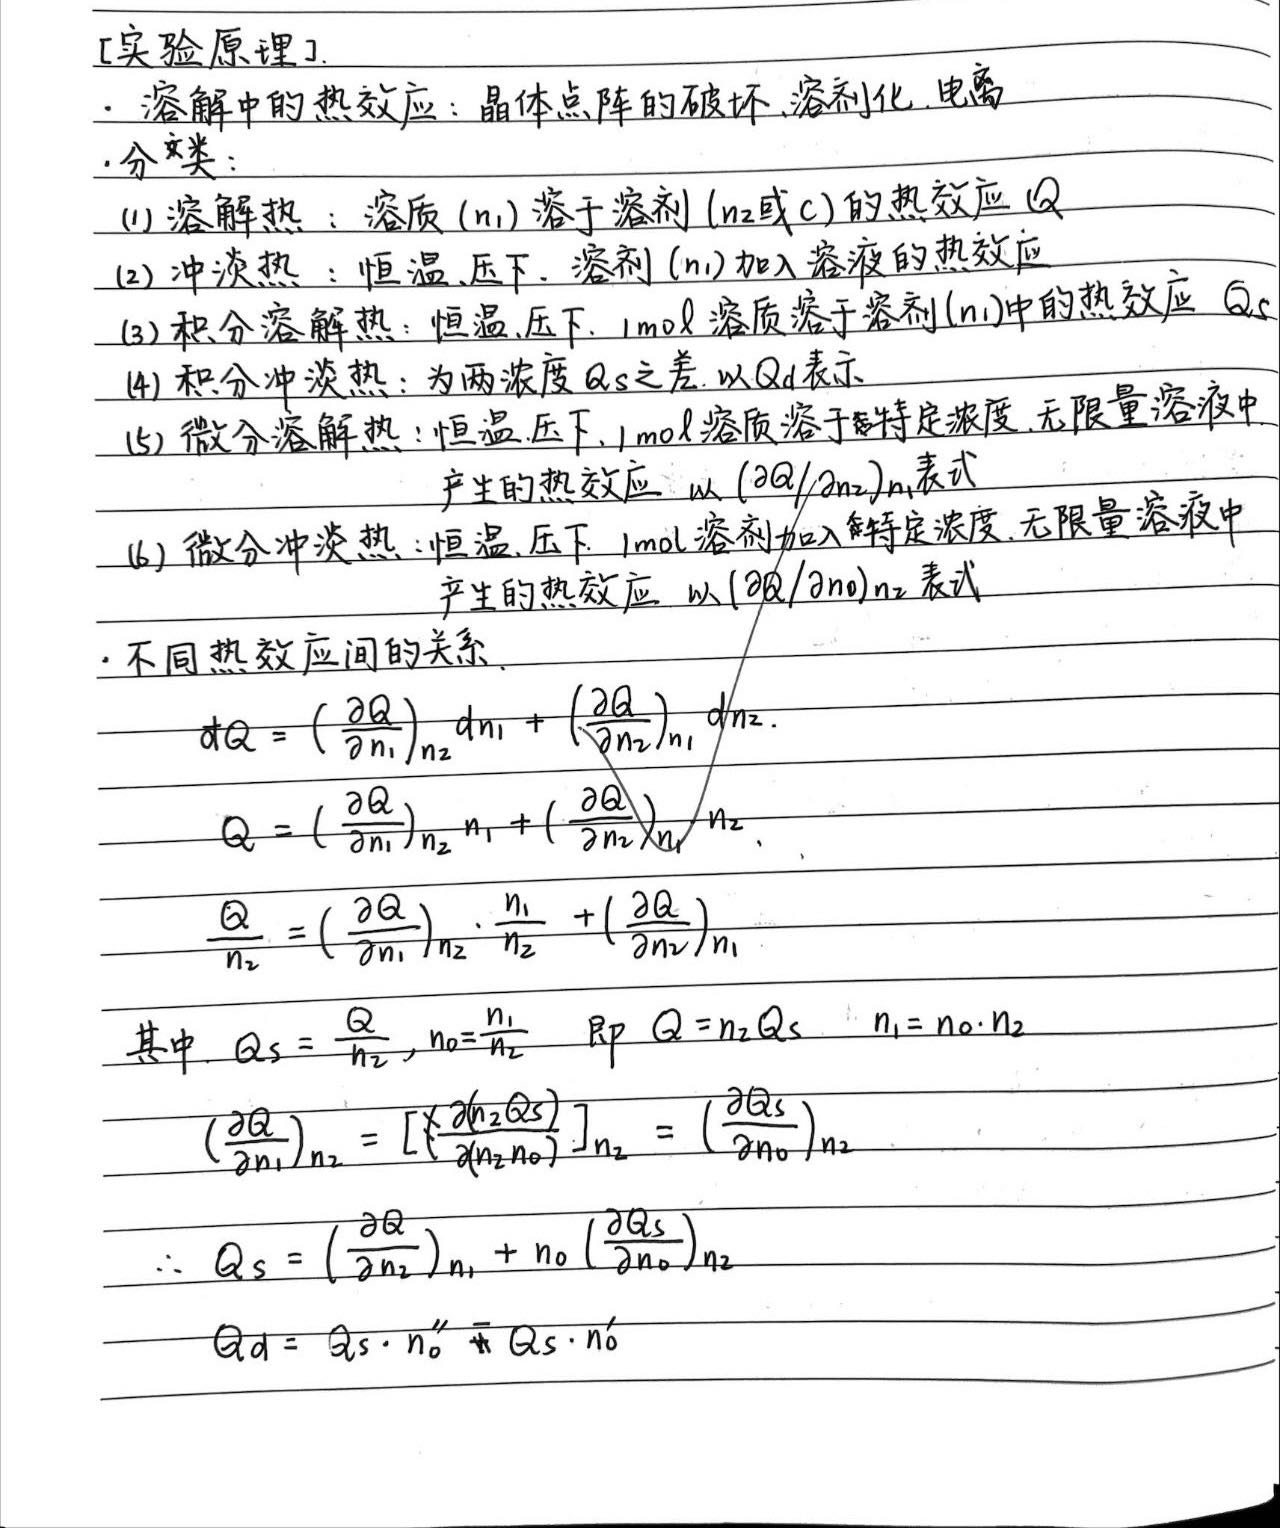
\includegraphics[width=0.75\textwidth]{figures/0-2.jpg}
    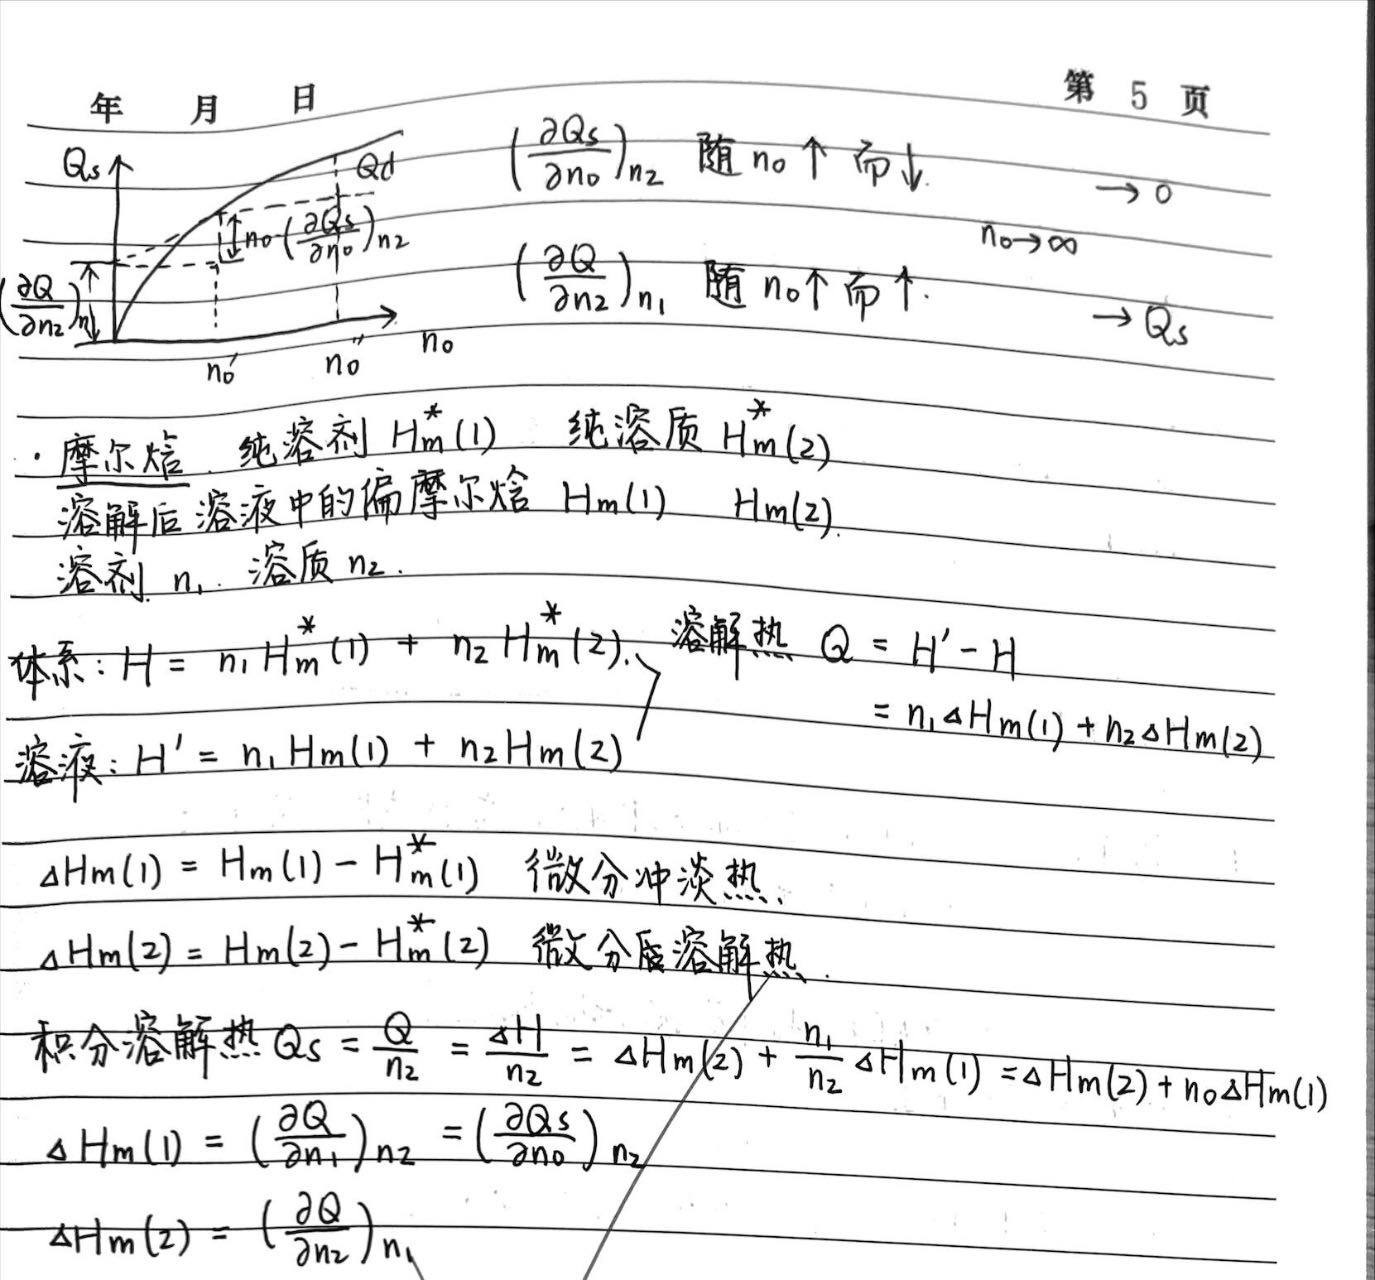
\includegraphics[width=0.75\textwidth]{figures/0-3.jpg}
    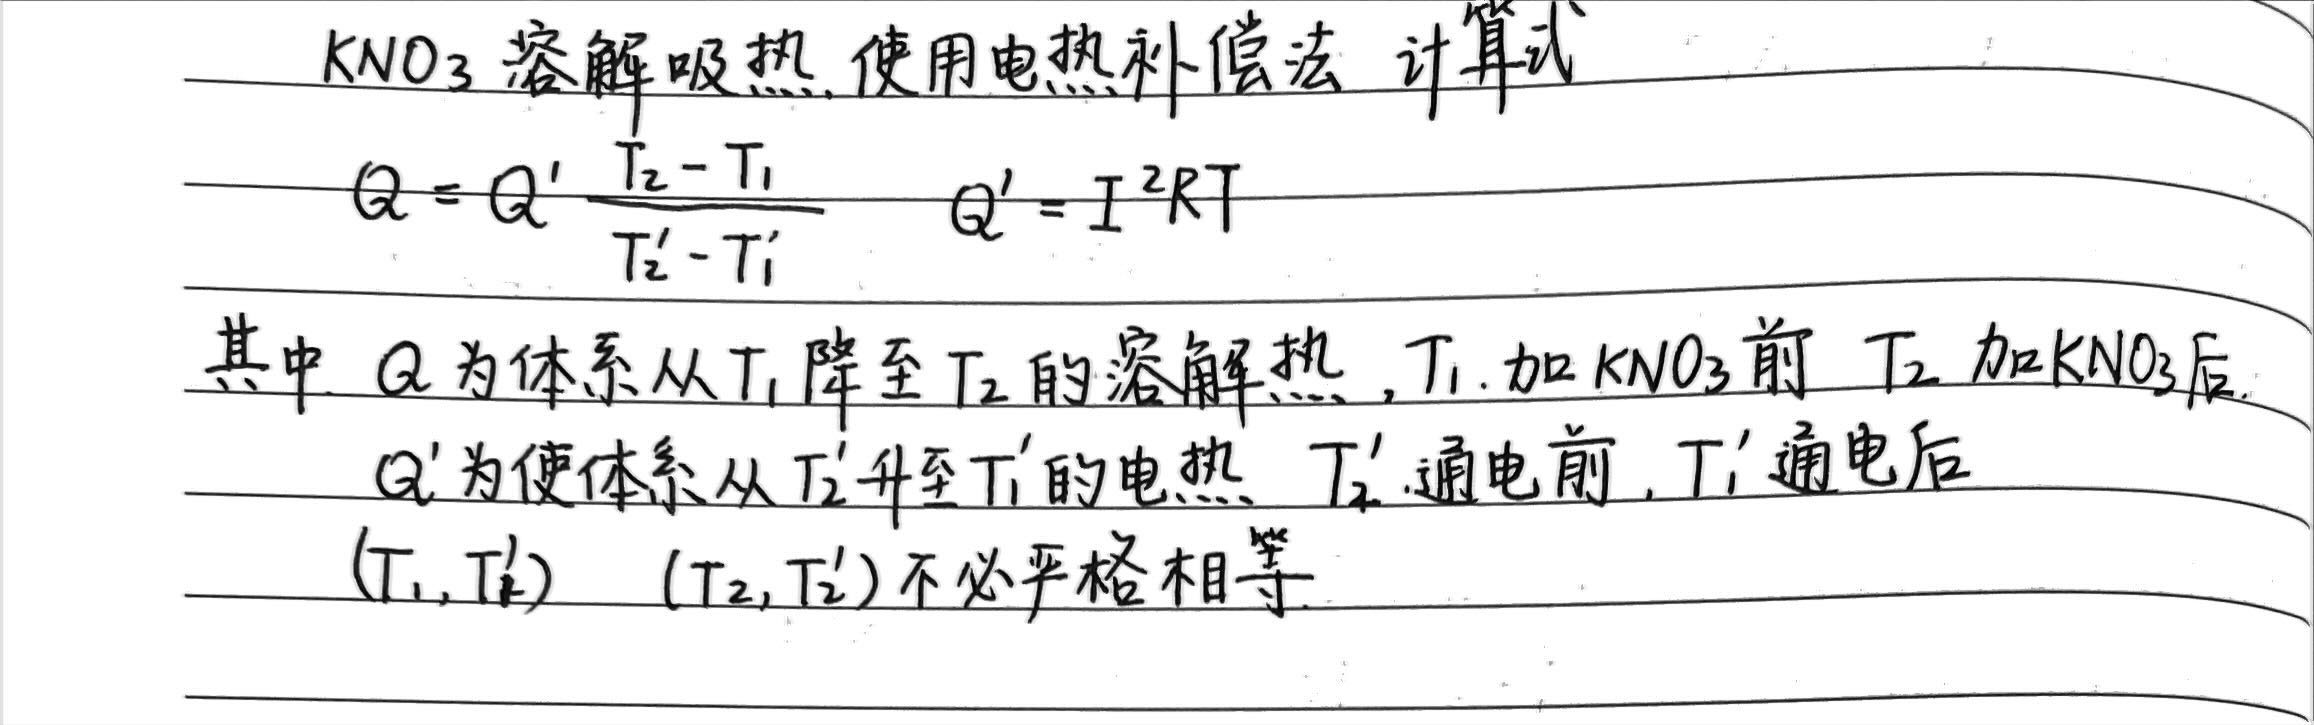
\includegraphics[width=0.75\textwidth]{figures/0-4.jpg}
    \caption{实验原理}
\end{figure}

\section{实验}

\subsection{主要仪器与药品}

\begin{figure}[htbp]
    \centering
    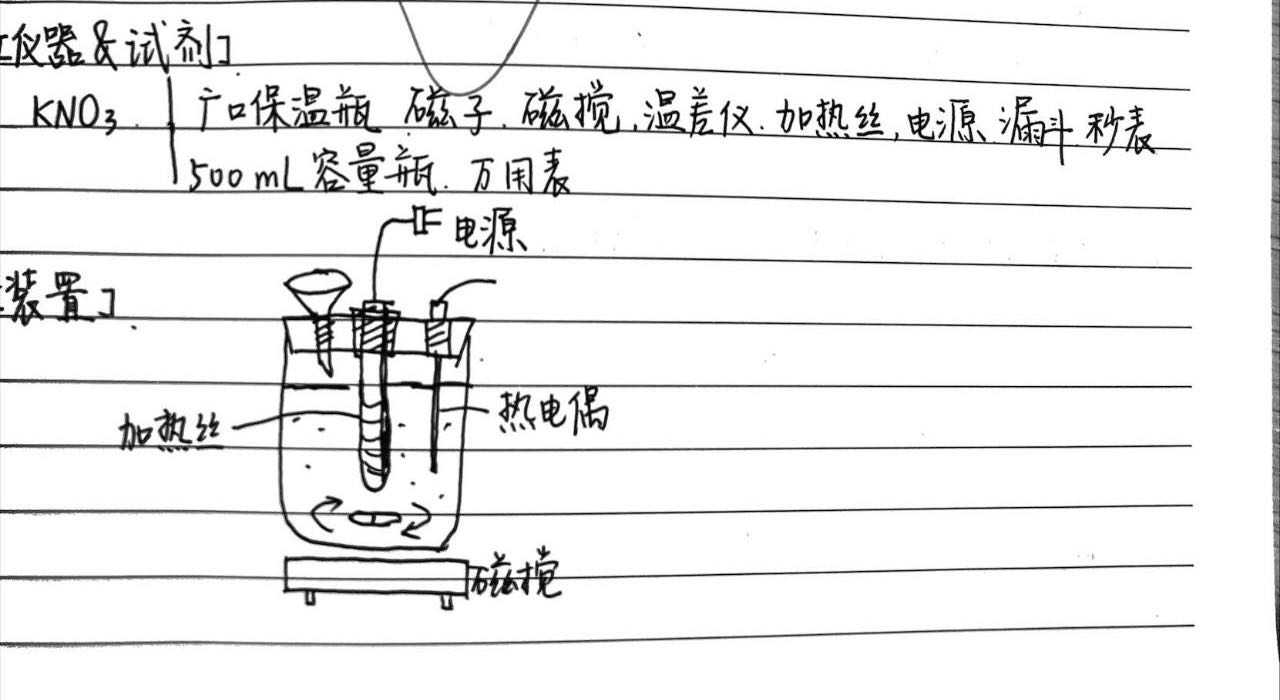
\includegraphics[width=0.9\textwidth]{figures/0-5.jpg}
    \caption{仪器与药品}
\end{figure}
%\begin{itemize}
    %\item \textbf{仪器}:广口保温瓶,磁子,电磁搅拌仪,数字温差仪,加热电阻丝,直流稳压电源,漏斗,秒表,500 \si{mL}容量瓶,万用表。
    %\item \textbf{药品}:\ce{KNO_3}(A.R.)。
%\end{itemize}

\subsection{实验步骤与条件}

\subsubsection{第一轮实验}

\begin{enumerate}
    \item 定容500 \si{mL}去离子水加入保温瓶中,搭建仪器联通线路,放入温差探测探头,测定加热电阻丝电阻,调节直流电源电流,使得功率在15$\sim$25 \si{W}附近,然后调节电压在额定电压以上。
    \item 准确称量18 \si{g}的\ce{KNO_3},打开搅拌,调零温差,开始记录,等待水温稳定。
    \item 用漏斗快速加入\ce{KNO_3},盖好盖子,降温等待温度进入平台期。
    \item 打开恒流电源开关,记录电流与时间,温度接近$T_1$时停止加热,记录通电时间,带热平衡后,再记录120 \si{s}组数据。
    \item 在\ce{KNO_3}溶液的基础上,再重复3遍步骤2$\sim$4。
\end{enumerate}

\subsubsection{第二轮实验}

\begin{enumerate}
    \item 更换定容500 \si{mL}去离子水加入保温瓶中,重复第一轮试验中的步骤。
    \item 调节电源电流至1.26 \si{A},调节磁力搅拌转速为2000 \si{rpm},重复六次实验,拟定每次加入\ce{KNO_3}的质量依次为9.00 \si{g}、9.25 \si{g}、9.50 \si{g}、9.75 \si{g}、10.00 \si{g}、10.25 \si{g},重复第一轮实验的步骤。
    \item 在第一次实验前与第六次实验后,分别测定加热电阻丝的电阻值。
\end{enumerate}

% 可以直接贴预习报告照片,也可以重写

\section{数据处理与结果呈现}

% 根据实验原理的要求对原始实验数据进行适当的处理并作出符合规范的图或表;对所作图、表作出必要的描述和说明;依据图、表得出该实验待测量的最终运算结果(注意有效数字)

\subsection{溶液浓度的计算}

此处“溶液的浓度”是指:溶液中溶剂与溶质的摩尔比$n_0$,即$n_0=\dfrac{n_1}{n_2}$,其计算公式如下
\begin{equation}
    n_0=\frac{n_1}{n_2}=\frac{\rho_{\ce{H_2O}}V_{\ce{H_2O}}/M_{\ce{H_2O}}}{m_{\ce{KNO_3}}/M_{\ce{KNO_3}}}=\frac{0.9973\times500/18.02}{m_{\ce{KNO_3}}/101.11} = \frac{2797.9}{m_{\ce{KNO_3}}}
    \label{eq:1}
\end{equation}
根据 \ref{eq:1} 可以计算得到每次加入\ce{KNO_3}后溶液的总浓度,两轮实验的溶液浓度分别如表 \ref{tab:1}、表 \ref{tab:2}。

\noindent
\begin{minipage}{0.499\textwidth}
  \centering
  \captionof{table}{第一轮实验的溶液浓度$n_0$}
  \label{tab:1}
  \begin{tabular}{ccc}
    \toprule
    $\Delta m$/g & $m$/g & $n_0$\\
    \midrule
    18.0075 & 18.0075 & 155.37\\
    18.0007 & 36.0082 & 77.70\\
    18.0045 & 54.0127 & 54.80\\
    18.0010 & 72.0137 & 38.85\\
    \bottomrule
  \end{tabular}
\end{minipage}%
\begin{minipage}{0.499\textwidth}
  \centering
  \captionof{table}{第二轮实验的溶液浓度$n_0$}
  \label{tab:2}
  \begin{tabular}{ccc}
    \toprule
    $\Delta m$/g & $m$/g & $n_0$\\
    \midrule
    9.0063 & 9.0063 & 310.66\\
    9.2567 & 18.2630 & 153.20\\
    9.5020 & 27.7650 & 100.77\\
    9.7516 & 37.5166 & 75.58\\
    10.0088 & 47.5254 & 58.87\\
    10.2516 & 57.7770 & 48.43\\
    \bottomrule
  \end{tabular}
\end{minipage}

\subsection{体系温度与时间的关系}

实验过程中使用 \href{https://github.com/ZhaoZh02}{ZhaoZh02}(赵泽华、安孝彦) 提供的\href{https://github.com/ZhaoZh02/Dissolution-Combustion}{软件}记录数据,两轮实验的体系温度-时间关系图分别如图\ref{fig:1}、\ref{fig:2}。原始数据见附录。

\begin{figure}[htbp]
    \centering
    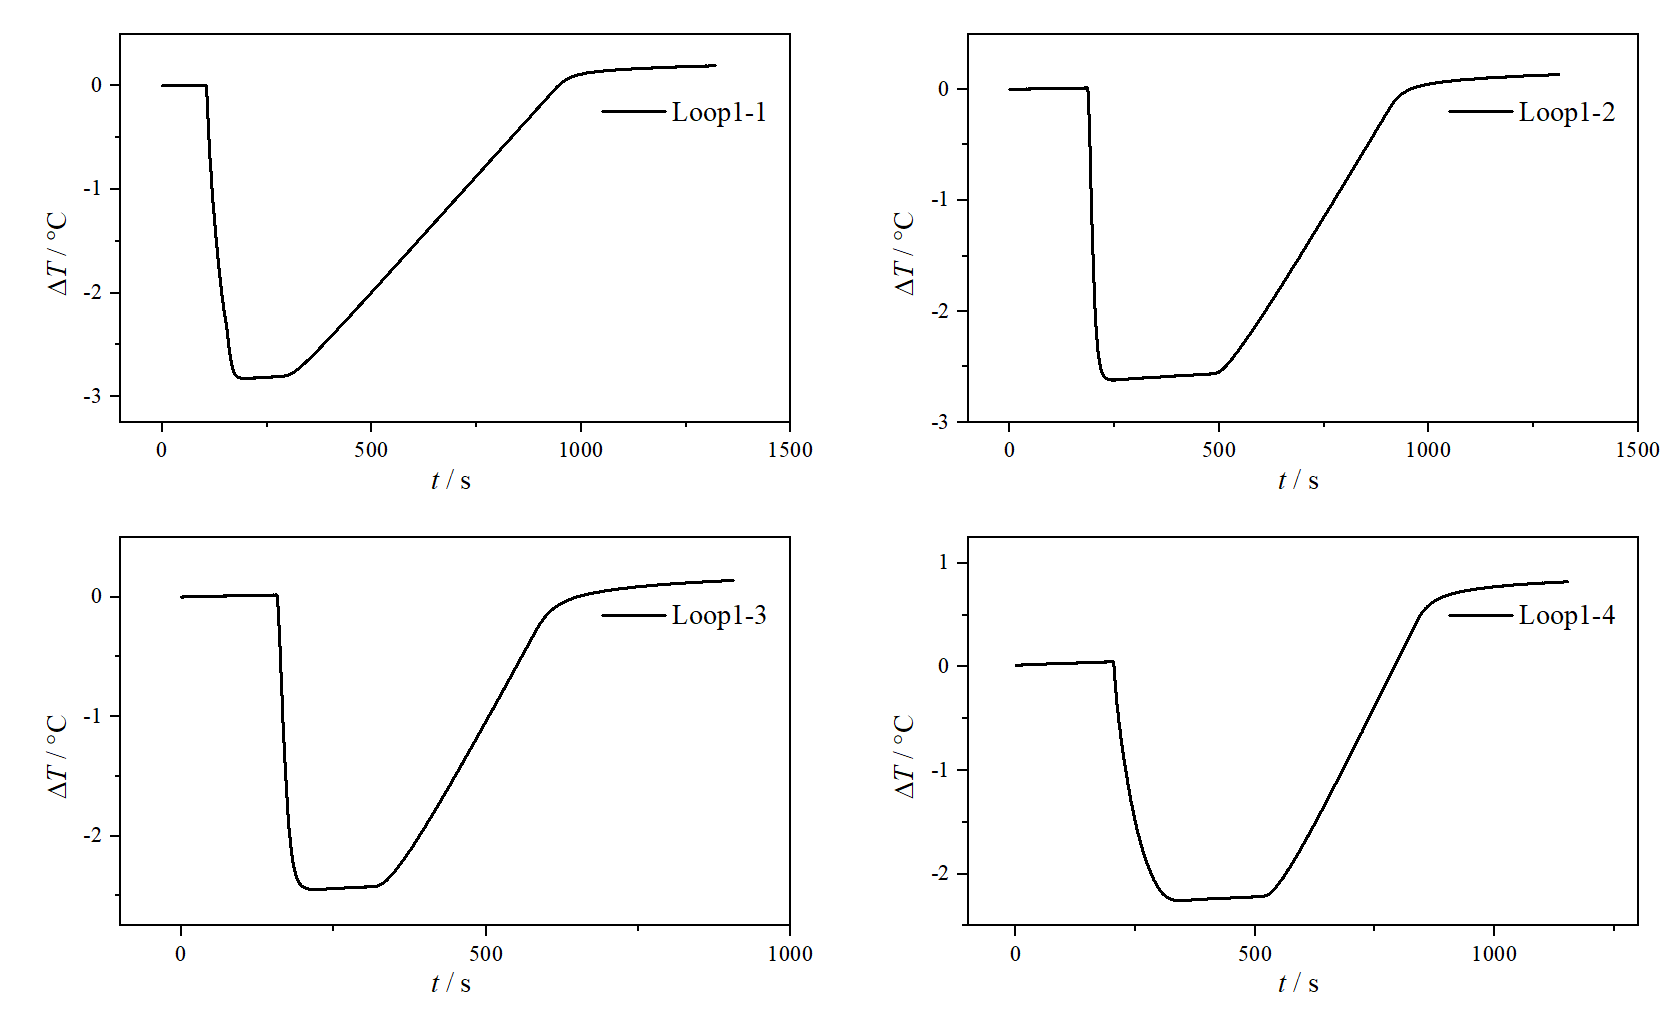
\includegraphics[width=.9\textwidth]{figures/1-1.png}
    \caption{第一轮实验的体系温度-时间关系}
    \label{fig:1}
\end{figure}
\begin{figure}[htbp]
    \centering
    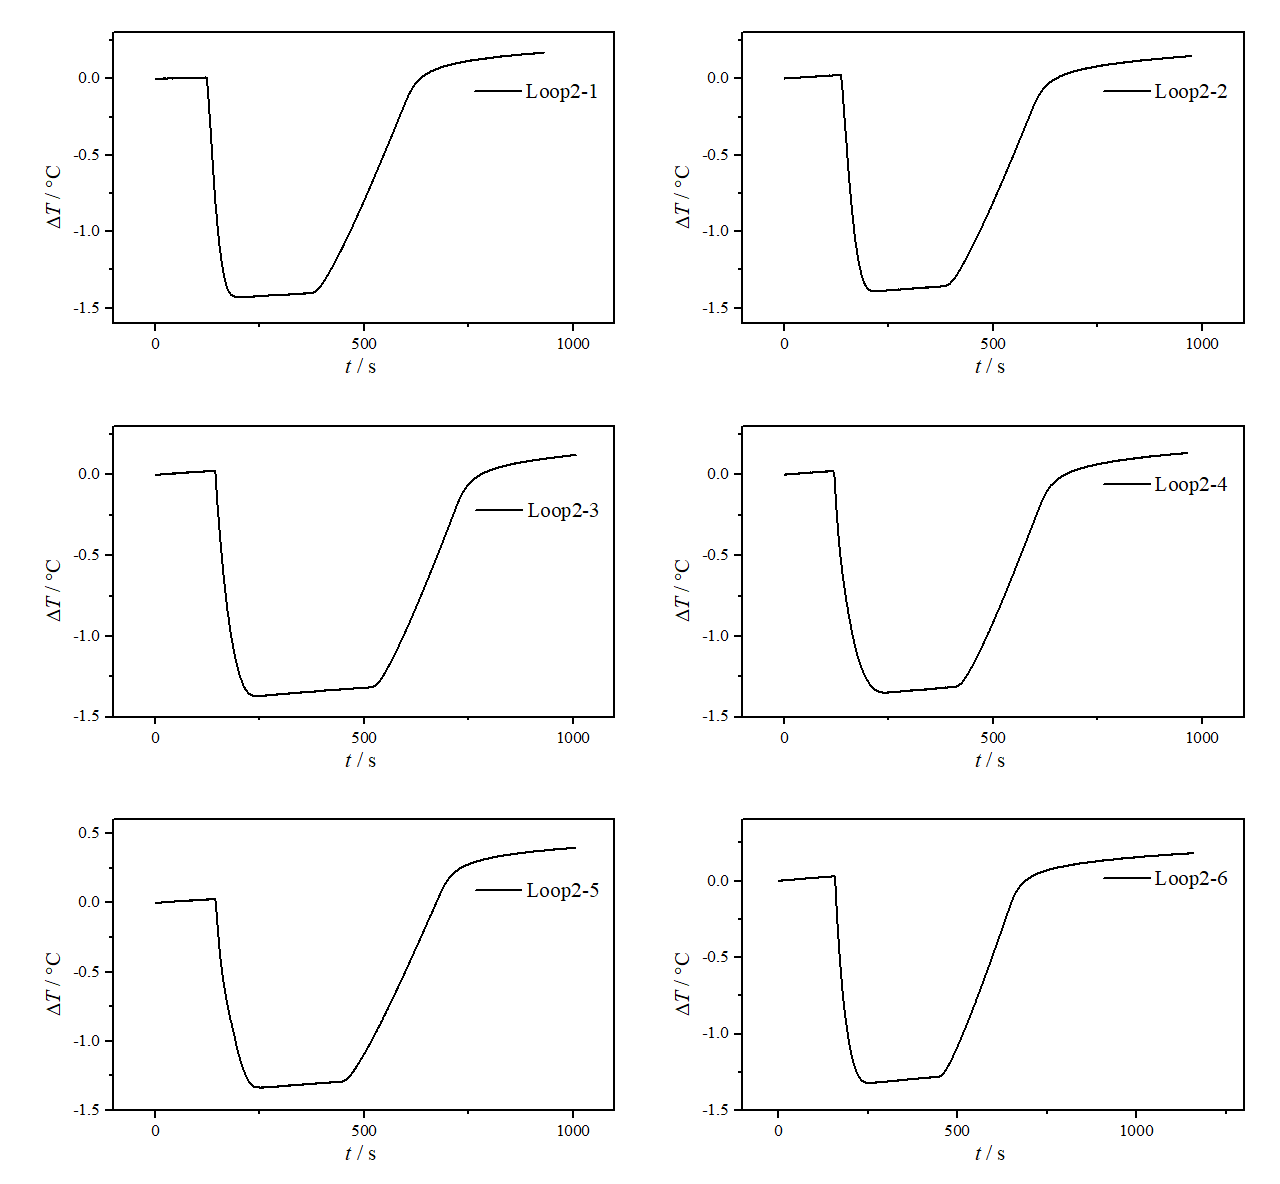
\includegraphics[width=.9\textwidth]{figures/1-2.png}
    \caption{第二轮实验的体系温度-时间关系}
    \label{fig:2}
\end{figure}

\subsection{雷诺校正确定温度与温度差}
使用使用 \href{https://github.com/ZhaoZh02}{ZhaoZh02}(赵泽华、安孝彦) 提供的\href{https://github.com/ZhaoZh02/Dissolution-Combustion}{数据处理工具}对实验的温度-时间关系进行雷诺校正,确定两轮实验降温、升温两个过程各自的起止时间$T_1,T_2,T_2^\prime,T_1^\prime$如表 \ref{tab:3},拟合直线如表 \ref{tab:4},得到的雷诺校正图如图 \ref{fig:3}、图 \ref{fig:4}。

\begin{table}[htbp]
    \centering
    \caption{雷诺校正得到的时间与温度、温度差}
    \begin{tabular}{ccccccccc}
        \toprule
        实验序号 & $t_a/\mathrm{S}$ & $T_1/\mathrm{{}^\circ C}$ & $T_2/\mathrm{{}^\circ C}$ & $\Delta T_a/\mathrm{{}^\circ C}$ & $t_b/\mathrm{S}$ & $T_2^\prime/\mathrm{{}^\circ C}$ & $T_1^\prime/\mathrm{{}^\circ C}$ & $\Delta T_b/\mathrm{{}^\circ C}$ \\
        \midrule
        Loop1-1 & 130.72 & 0.006 & -2.843  & 2.849 & 628.90 & -2.715 & 0.0080 & 2.795 \\
        Loop1-2 & 198.67 & 0.015 & -2.629  & 2.644 & 734.63 & -2.501 & 0.027 & 2.528 \\
        Loop1-3 & 170.16 & 0.021 & -2.461  & 2.482 & 485.23 & -2.370 & 0.017 & 2.387 \\
        Loop1-4 & 240.86 & 0.056 & -2.280  & 2.336 & 711.60 & -2.167 & 0.704 & 2.871 \\
        \midrule
        Loop2-1 & 143.91 & 0.010 & -1.439  & 1.449 & 522.99 & -1.375 & 0.065 & 1.440 \\
        Loop2-2 & 158.98 & 0.028 & -1.405  & 1.433 & 526.41 & -1.322 & 0.030 & 1.352 \\
        Loop2-3 & 170.16 & 0.030 & -1.386  & 1.416 & 654.39 & -1.285 & 0.012 & 1.297 \\
        Loop2-4 & 149.29 & 0.030 & -1.371  & 1.401 & 546.43 & -1.283 & 0.022 & 1.305 \\
        Loop2-5 & 174.17 & 0.034 & -1.353  & 1.387 & 600.47 & -1.256 & 0.286 & 1.542 \\
        Loop2-6 & 181.37 & 0.036 & -1.337  & 1.373 & 587.16 & -1.248 & 0.085 & 1.333 \\
        \bottomrule
    \end{tabular}
    \label{tab:3}
\end{table}

\begin{figure}[htbp]
    \centering
    \begin{subfigure}{0.45\textwidth}
        \centering
        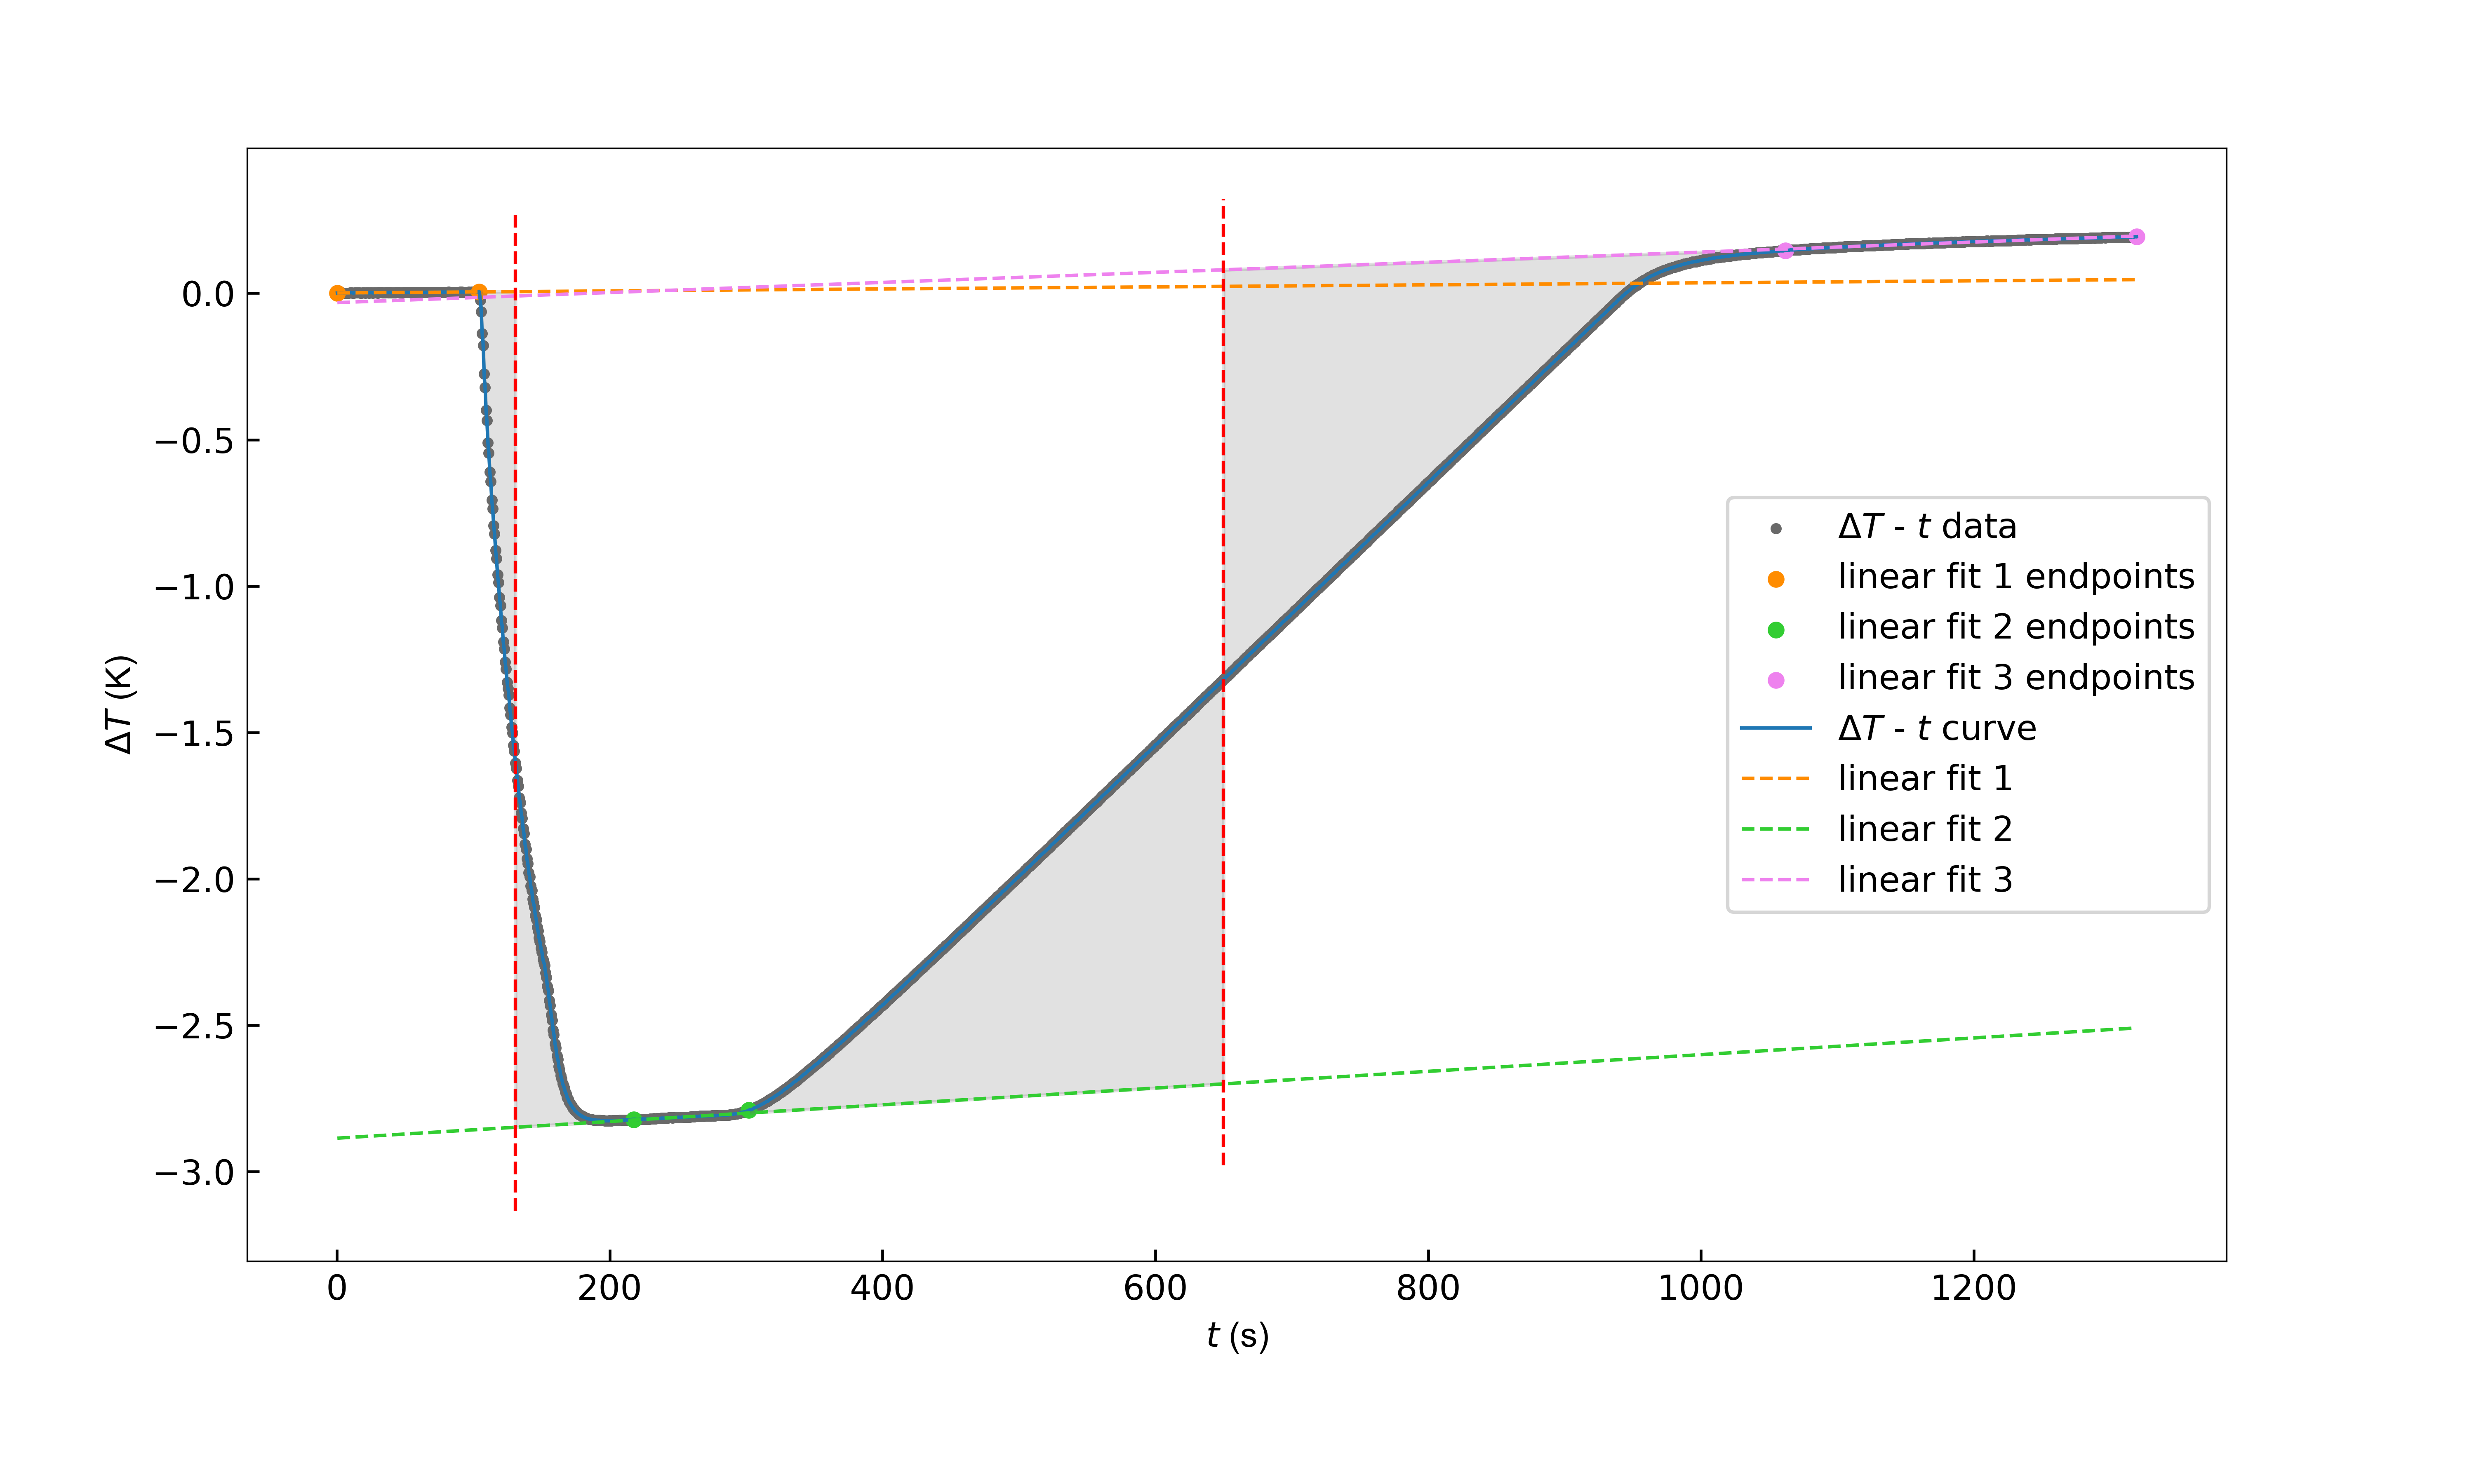
\includegraphics[width=\linewidth]{figures/2-1.png}
        \caption*{Loop1-1}
    \end{subfigure}
    \hfill
    \begin{subfigure}{0.45\textwidth}
        \centering
        \includegraphics[width=\linewidth]{figures/2-2.png}
        \caption*{Loop1-2}
    \end{subfigure}
    \vspace{1em} % Adjust the vertical spacing as needed
    \begin{subfigure}{0.45\textwidth}
        \centering
        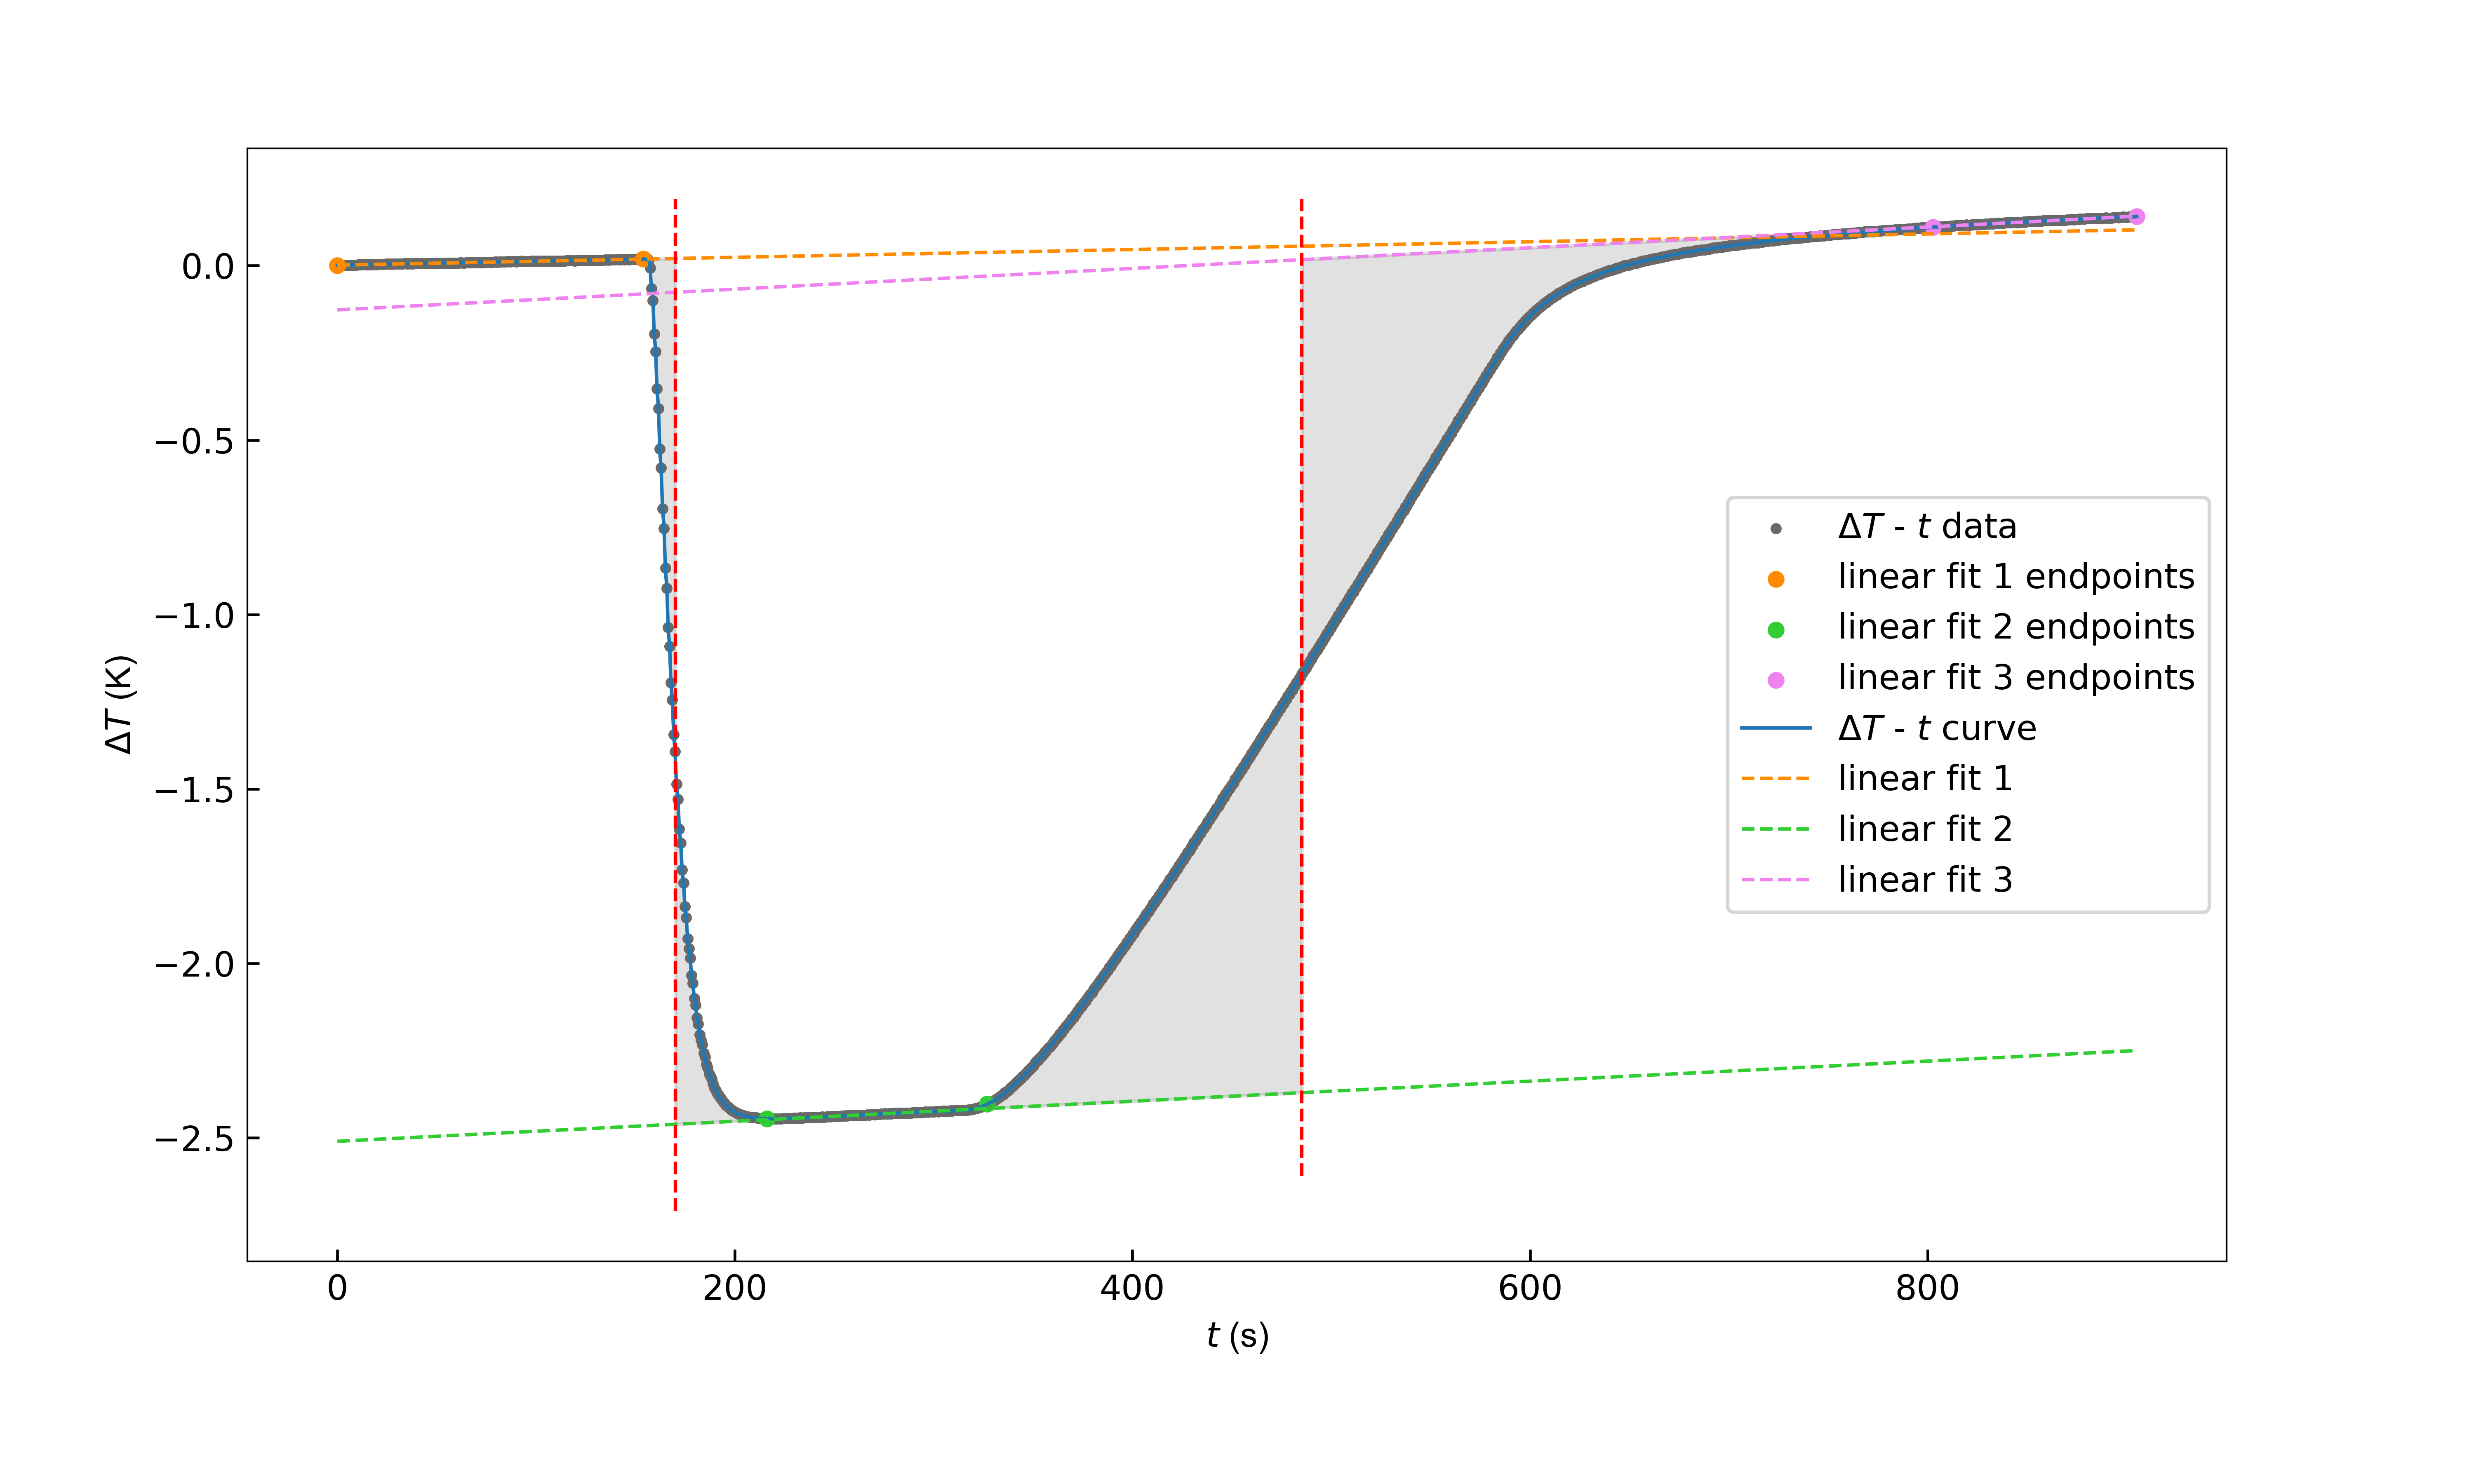
\includegraphics[width=\linewidth]{figures/2-3.png}
        \caption*{Loop1-3}
    \end{subfigure}
    \hfill
    \begin{subfigure}{0.45\textwidth}
        \centering
        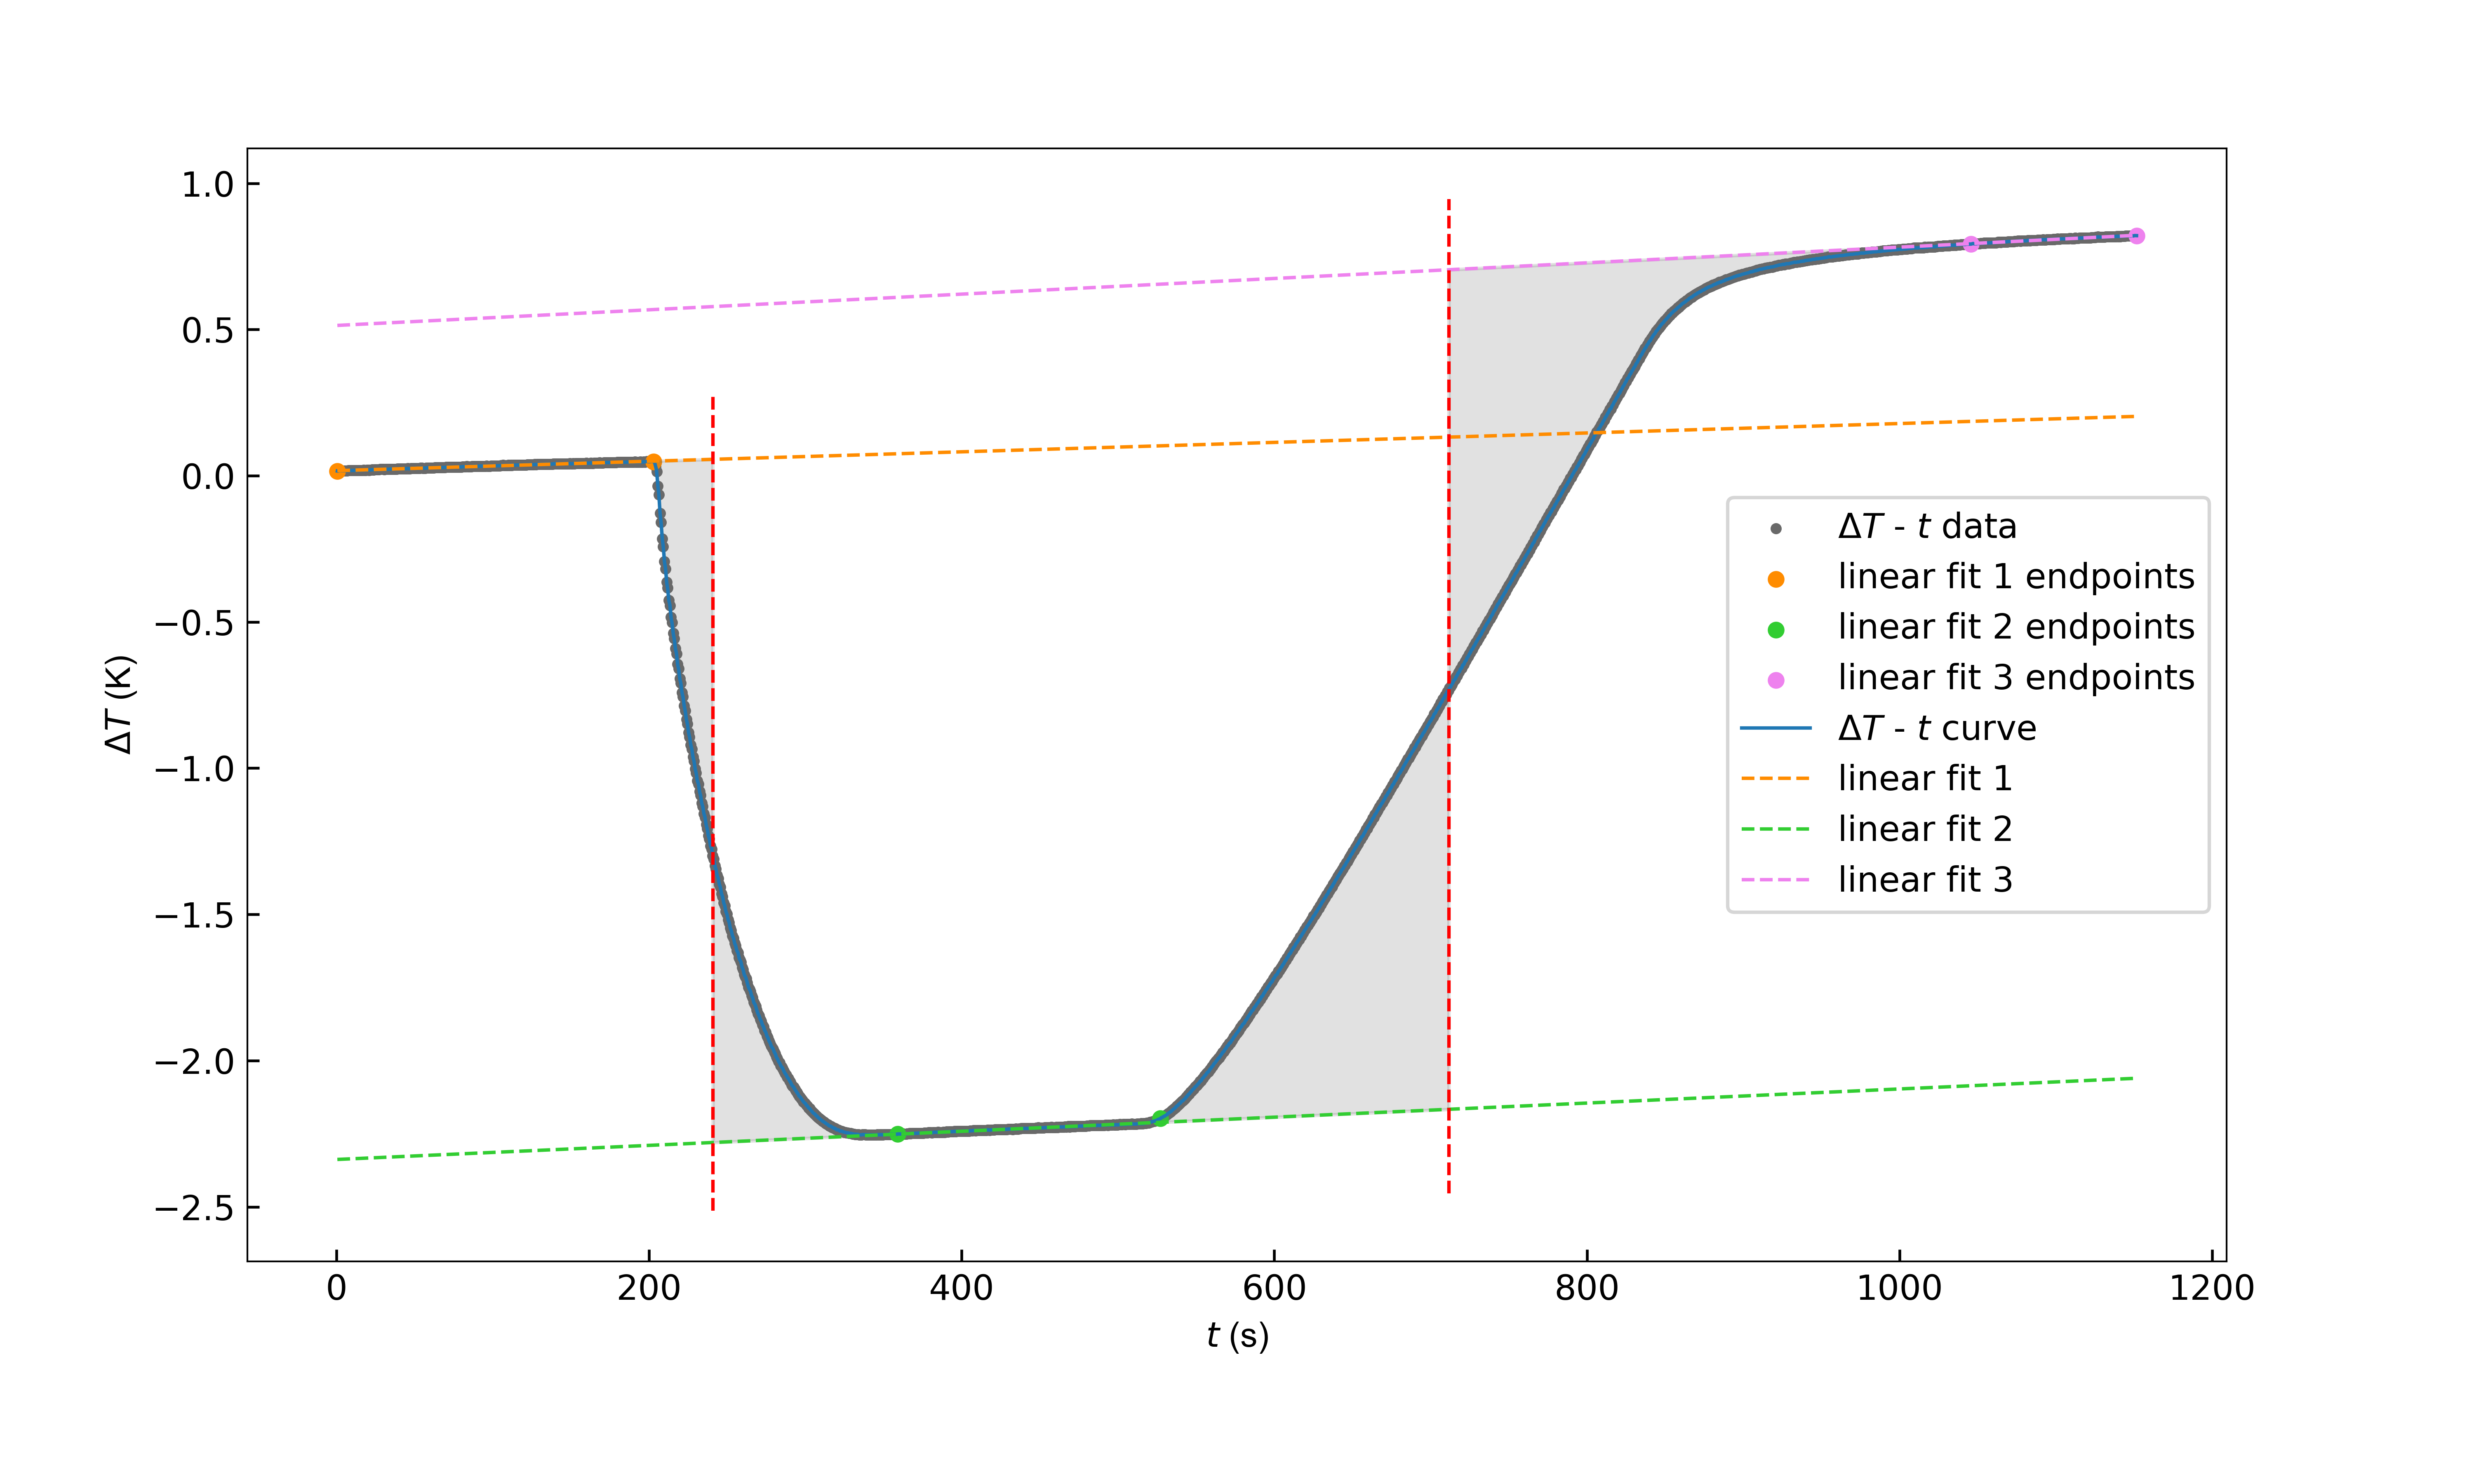
\includegraphics[width=\linewidth]{figures/2-4.png}
        \caption*{Loop1-4}
    \end{subfigure}
    \caption{第一轮实验的雷诺校正图}
    \label{fig:3}
\end{figure}

\begin{figure}[htbp]
    \centering
    \begin{subfigure}{0.45\textwidth}
        \centering
        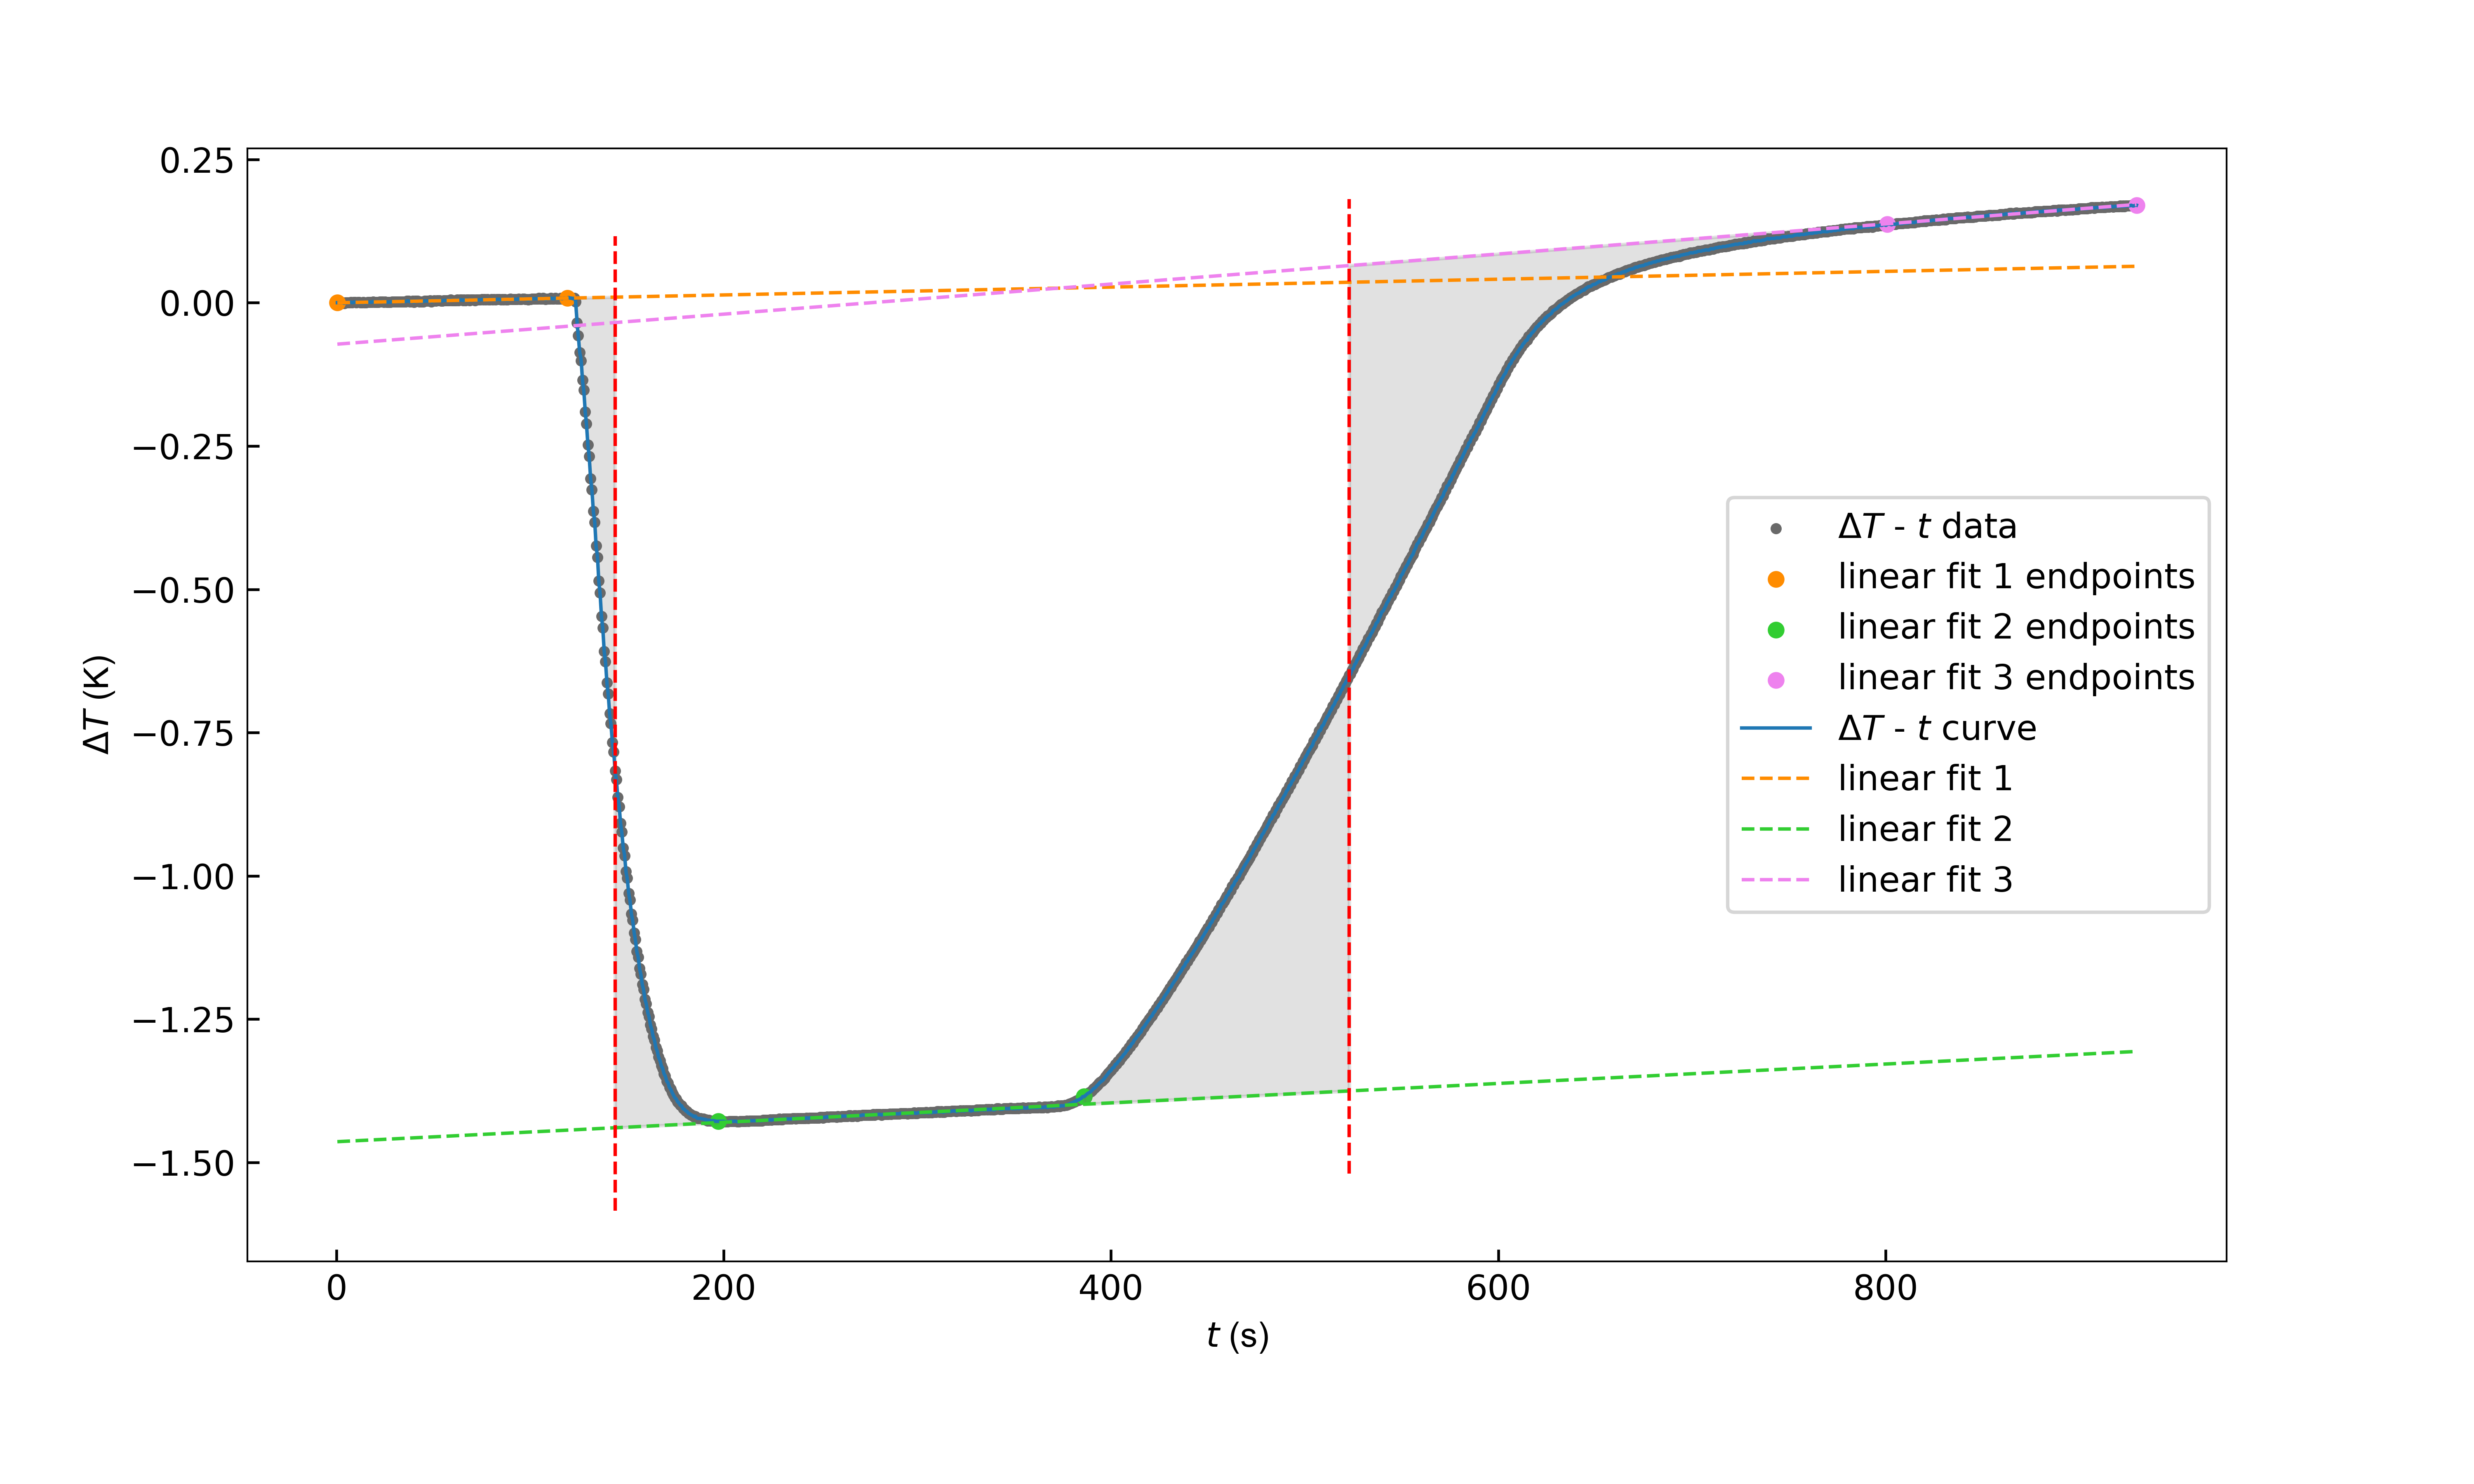
\includegraphics[width=\linewidth]{figures/3-1.png}
        \caption*{Loop2-1}
    \end{subfigure}
    \hfill
    \begin{subfigure}{0.45\textwidth}
        \centering
        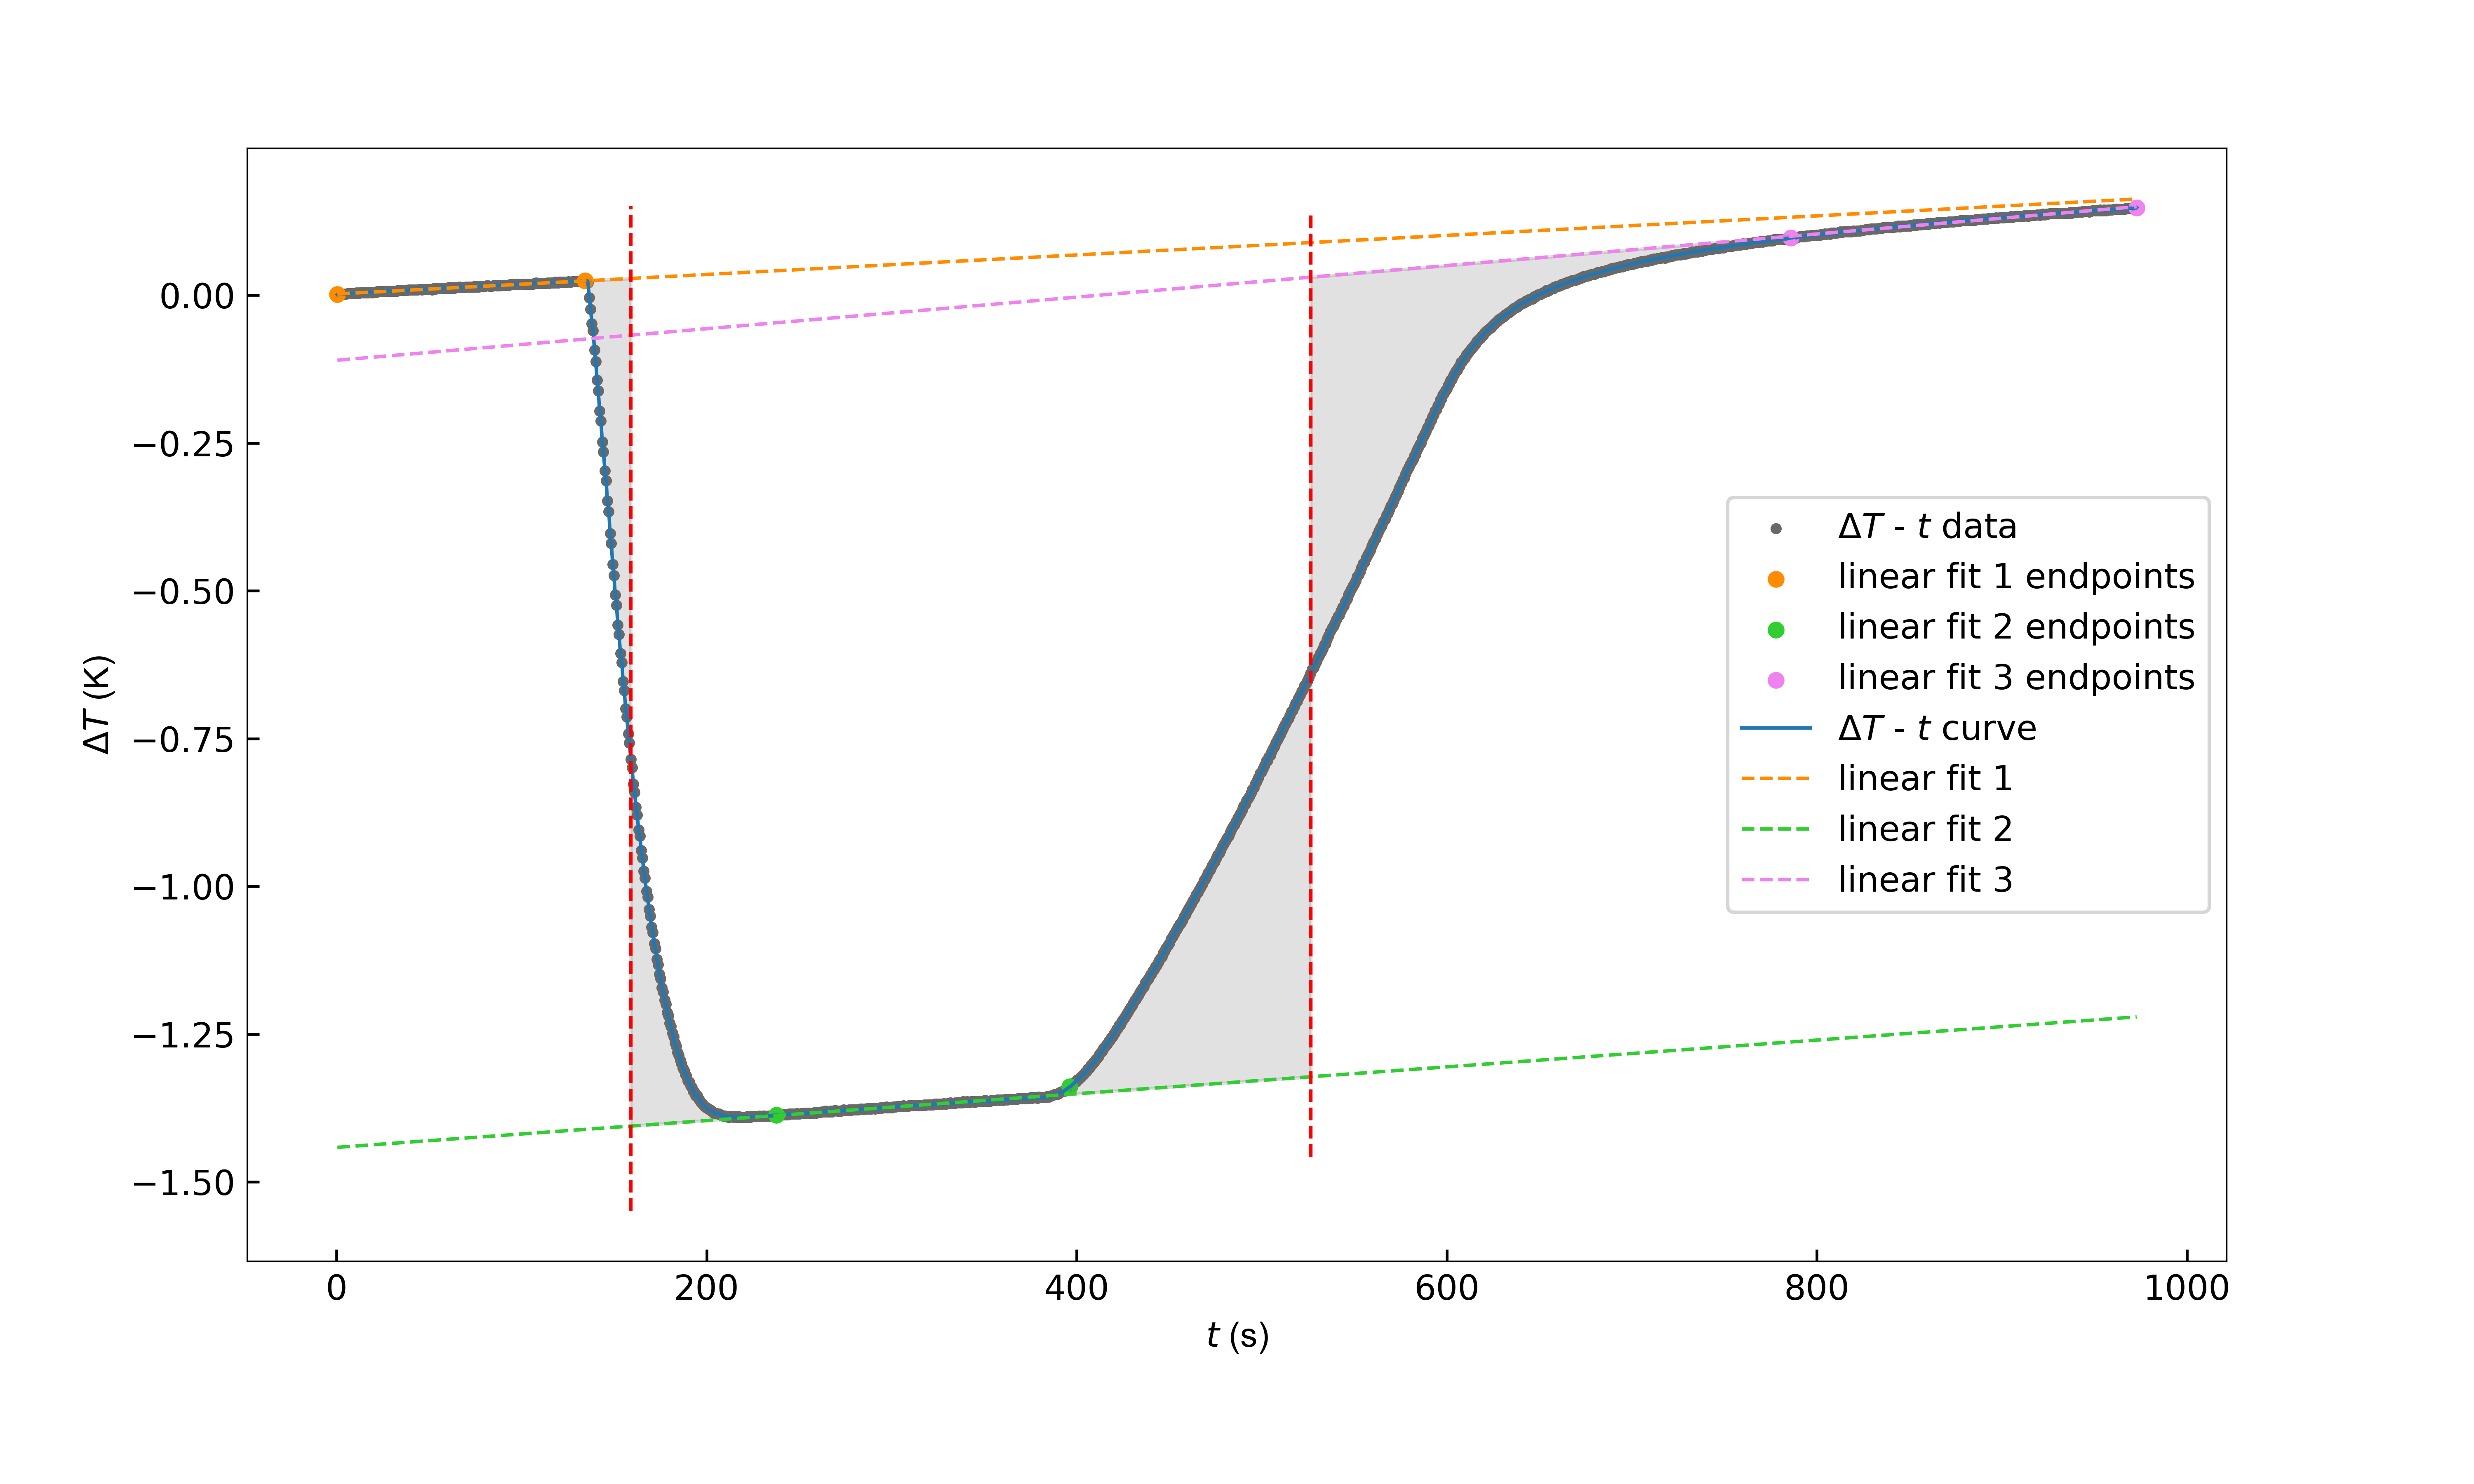
\includegraphics[width=\linewidth]{figures/3-2.png}
        \caption*{Loop2-2}
    \end{subfigure}
    \vspace{1em} % Adjust the vertical spacing as needed
    \begin{subfigure}{0.45\textwidth}
        \centering
        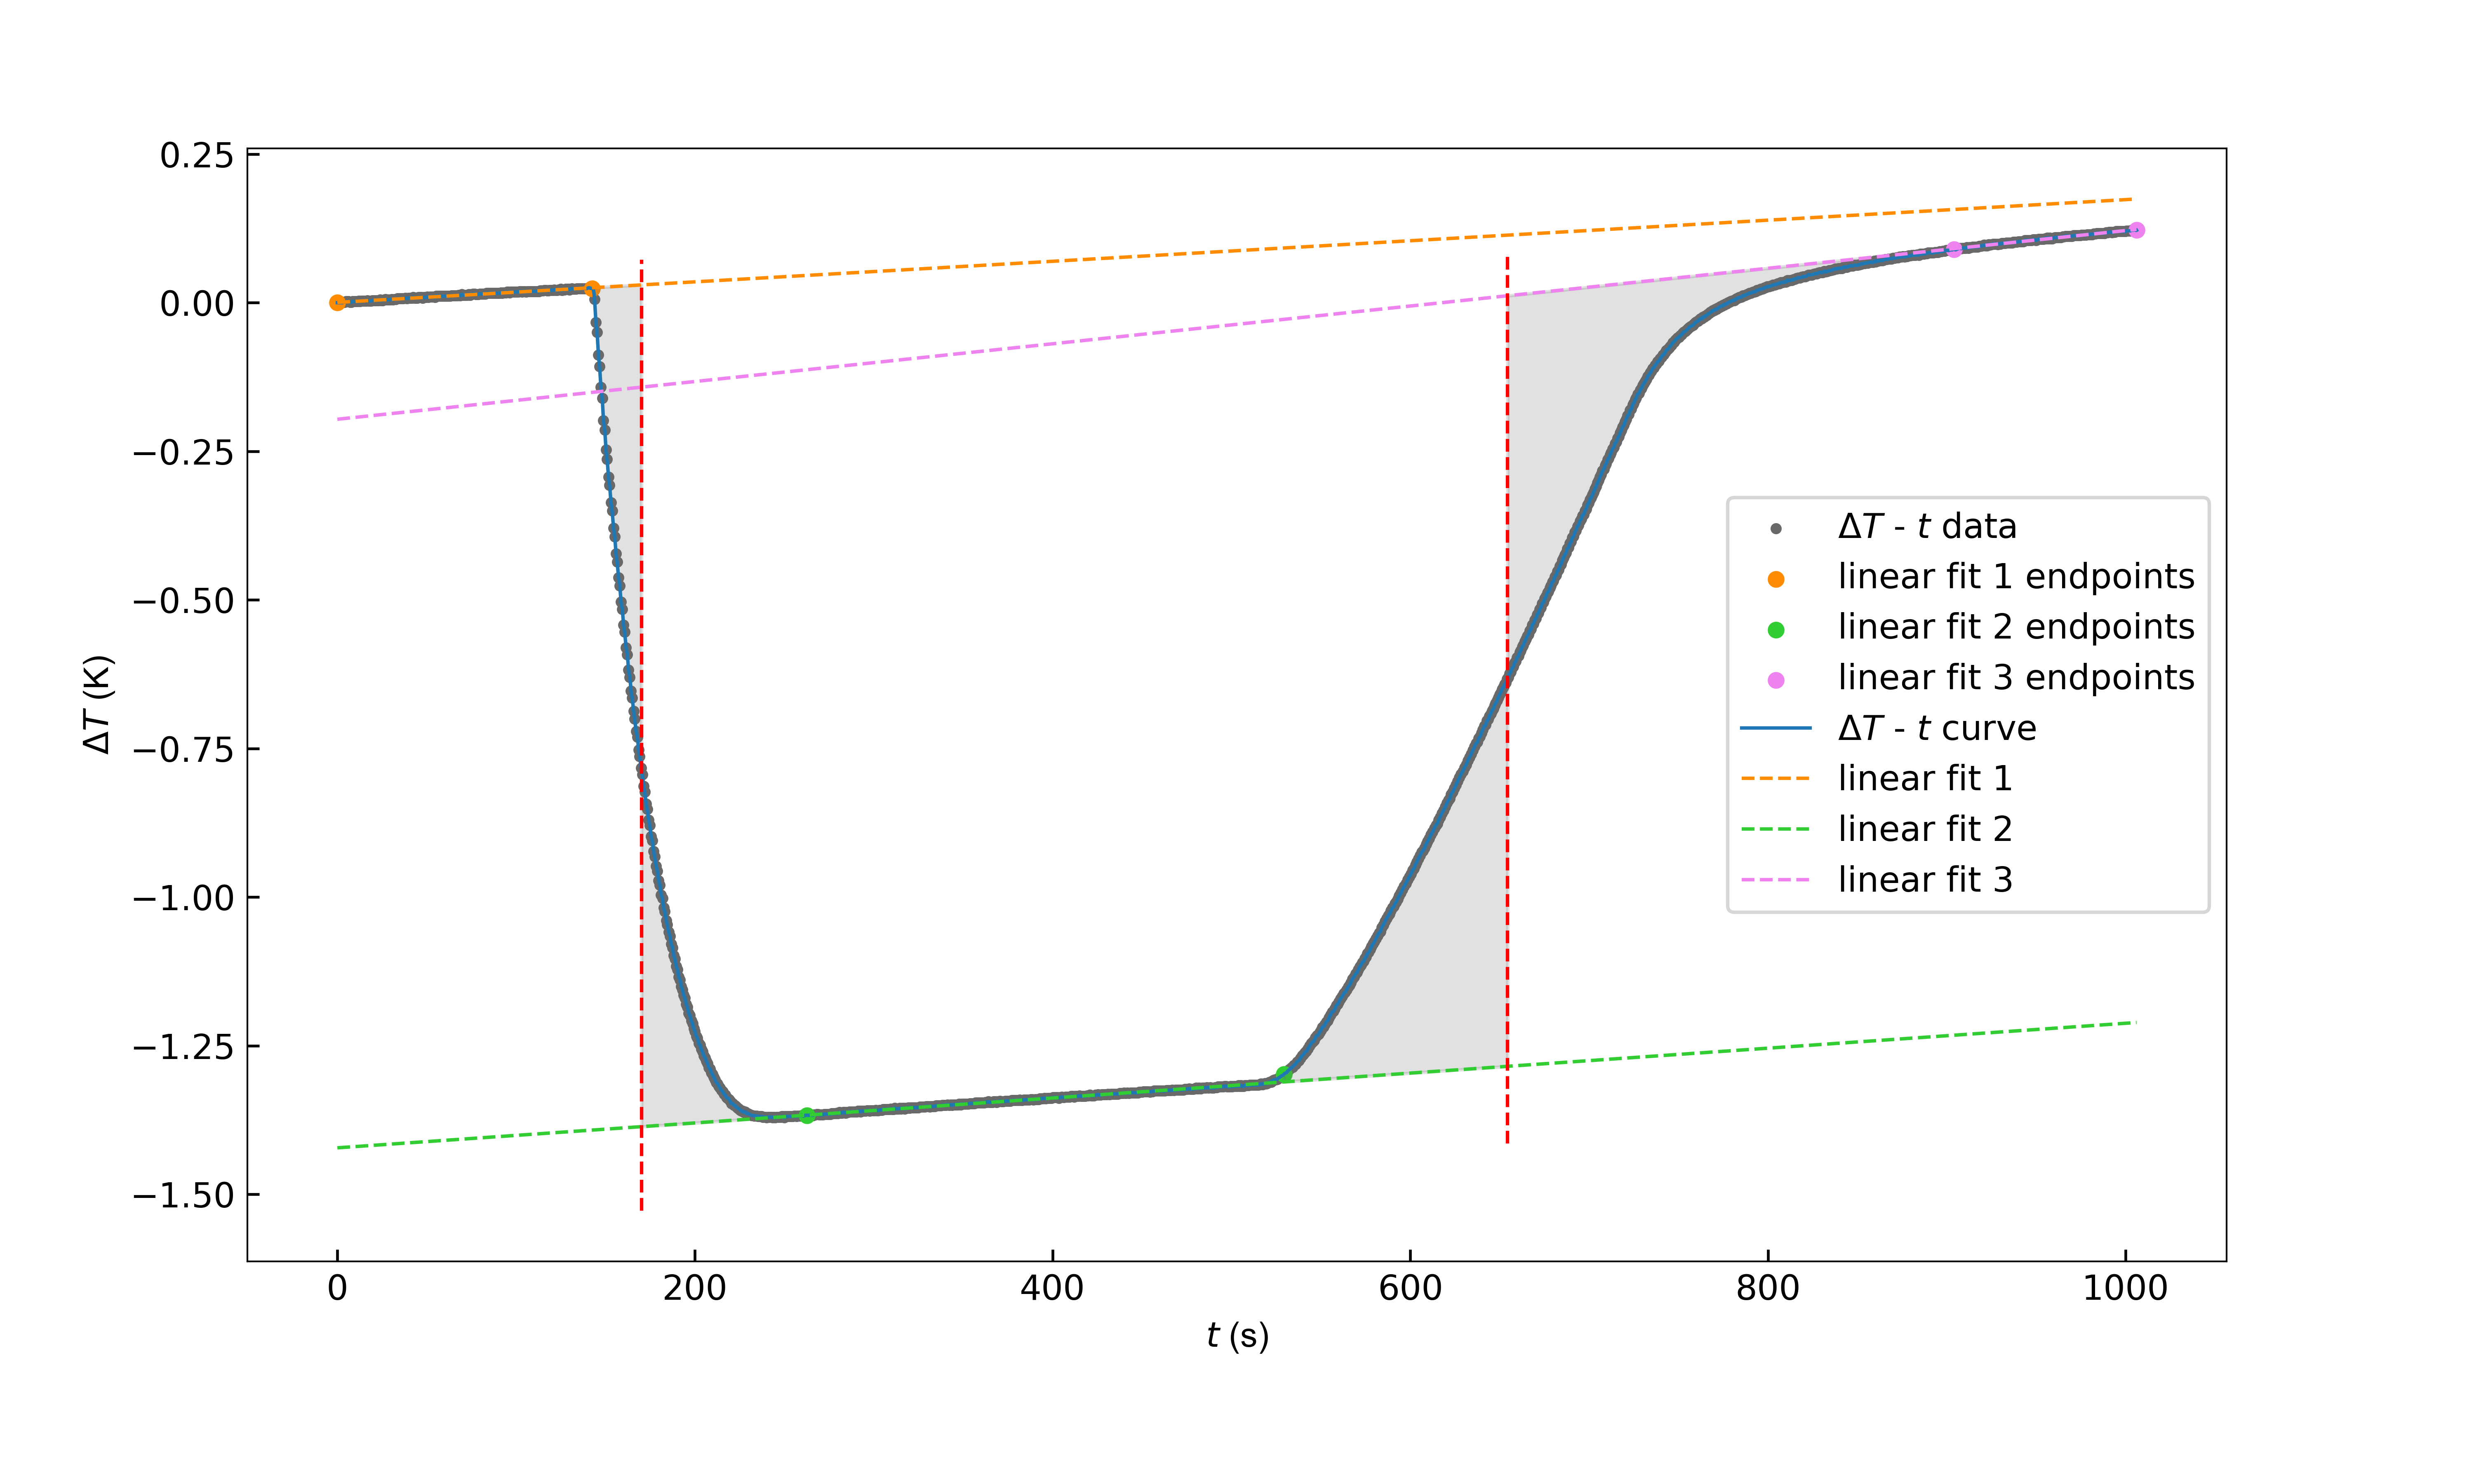
\includegraphics[width=\linewidth]{figures/3-3.png}
        \caption*{Loop2-3}
    \end{subfigure}
    \hfill
    \begin{subfigure}{0.45\textwidth}
        \centering
        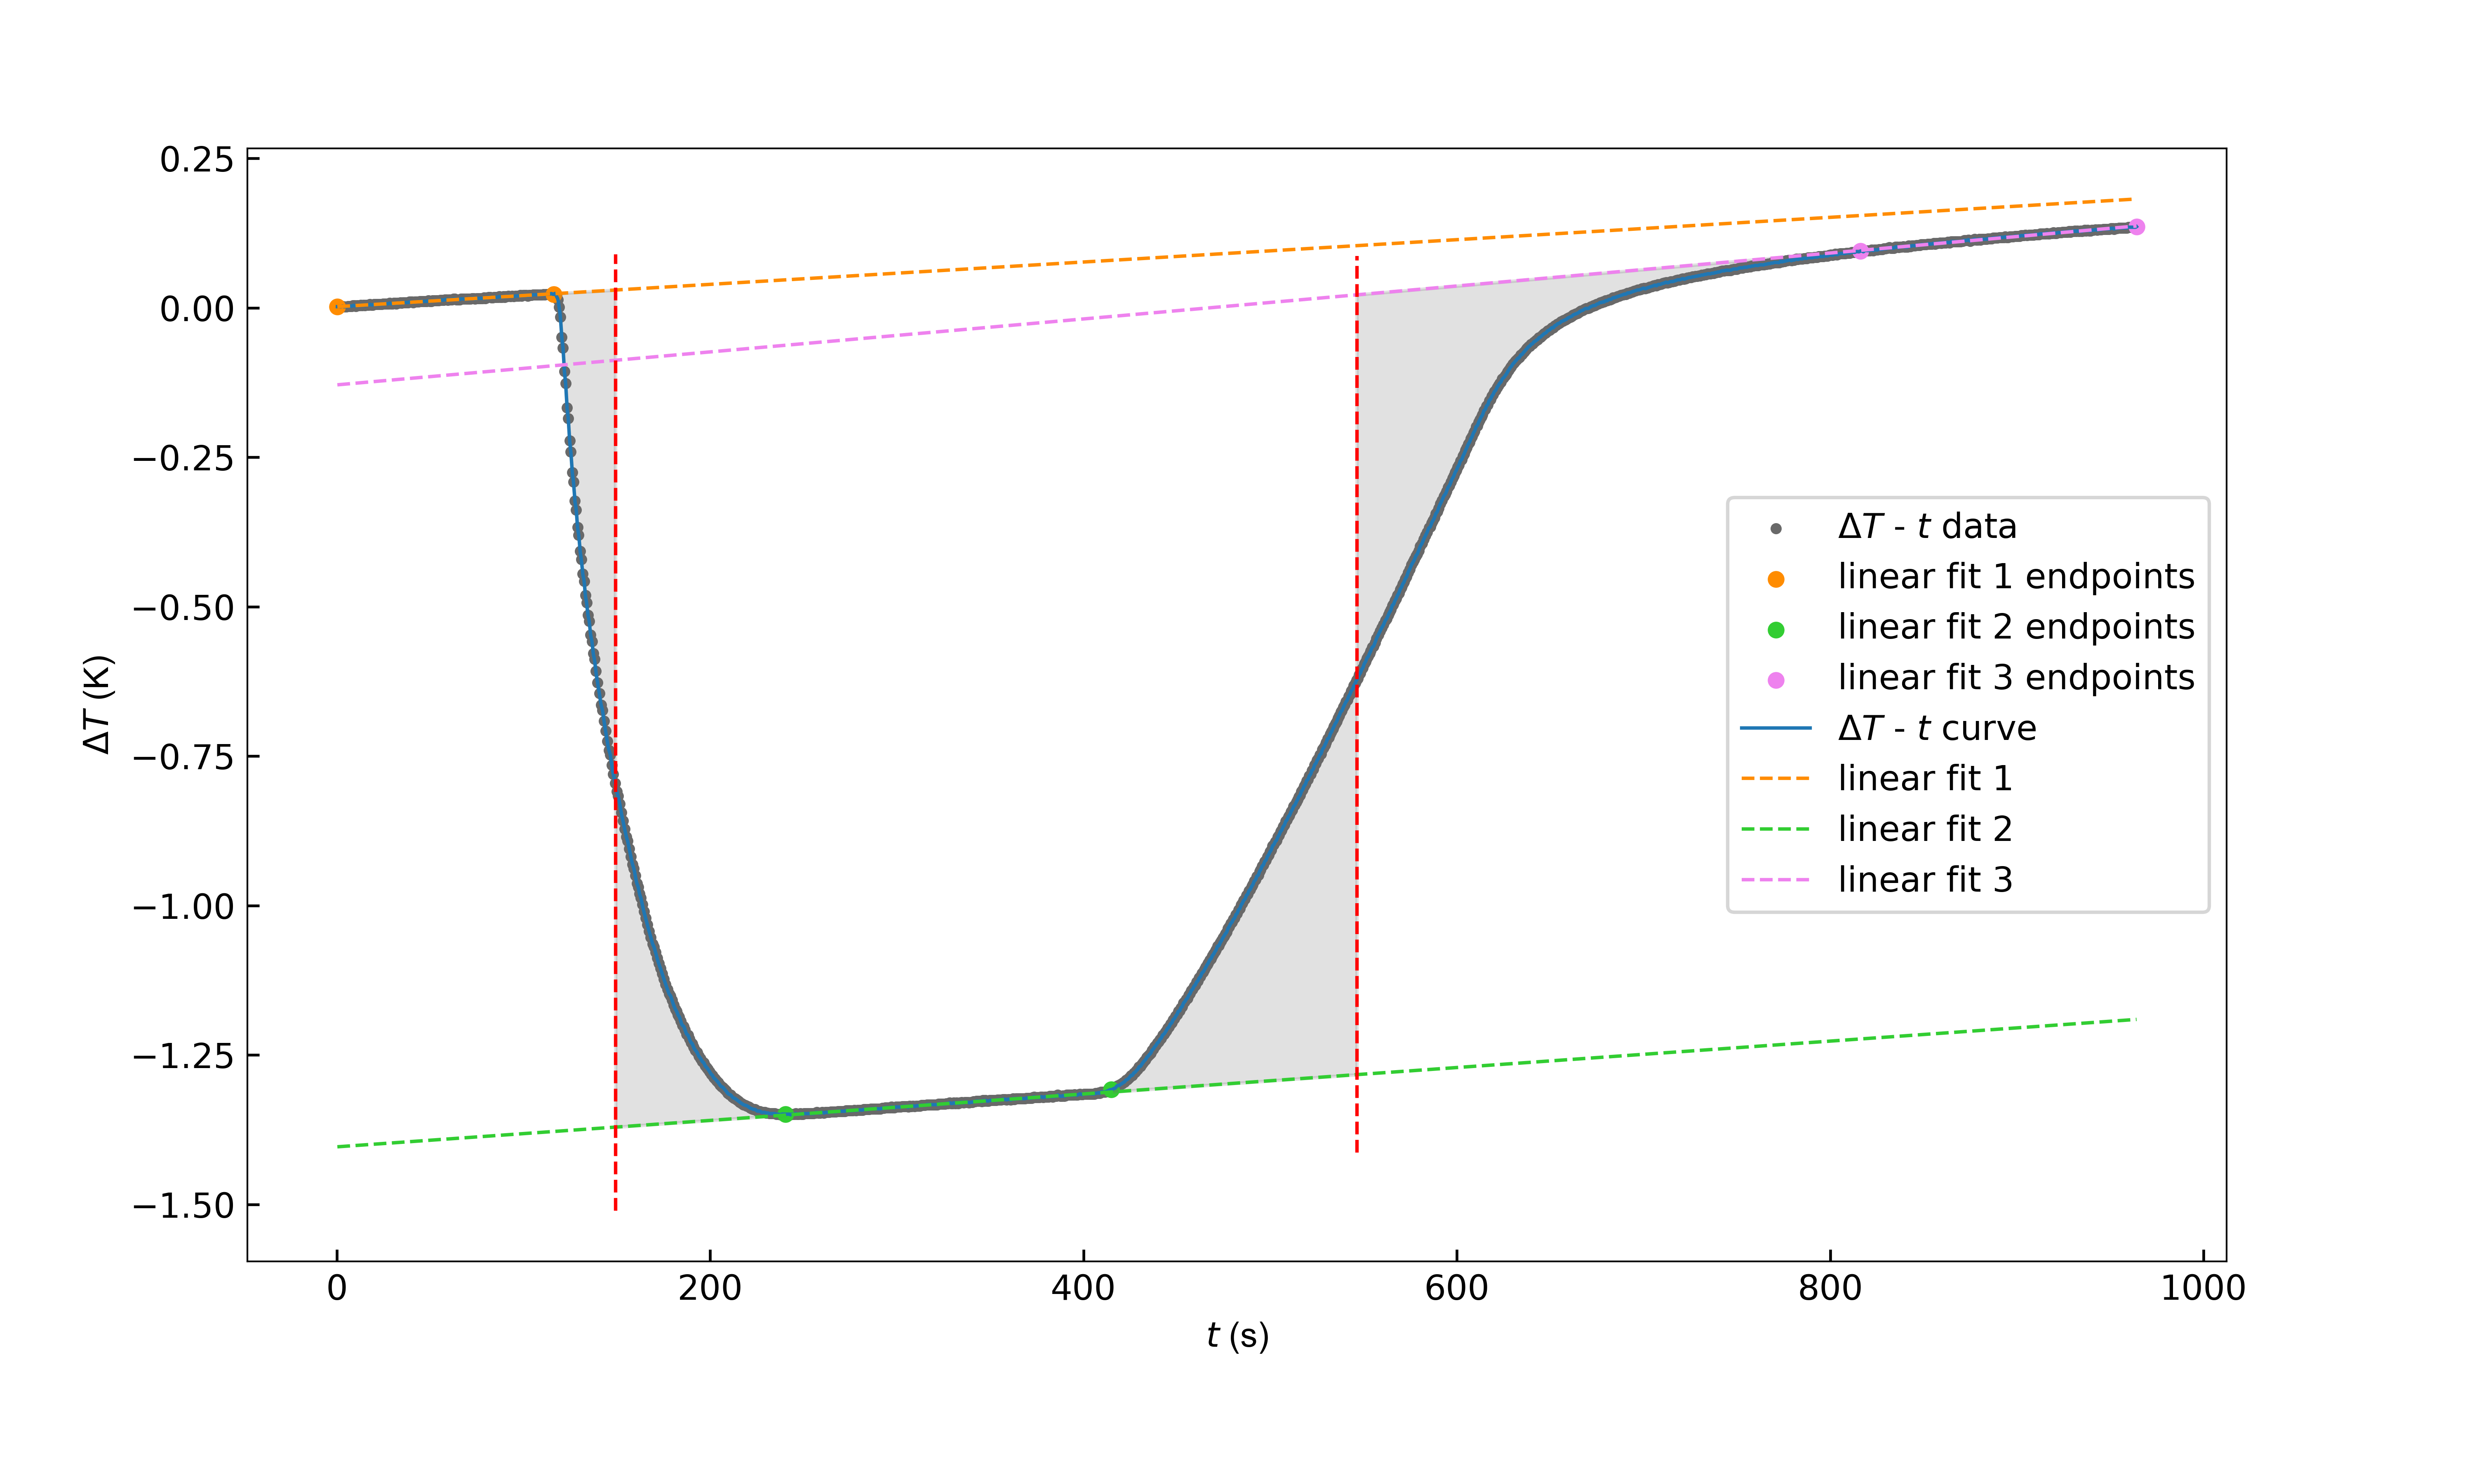
\includegraphics[width=\linewidth]{figures/3-4.png}
        \caption*{Loop2-4}
    \end{subfigure}
    \vspace{1em} % Adjust the vertical spacing as needed
    \begin{subfigure}{0.45\textwidth}
        \centering
        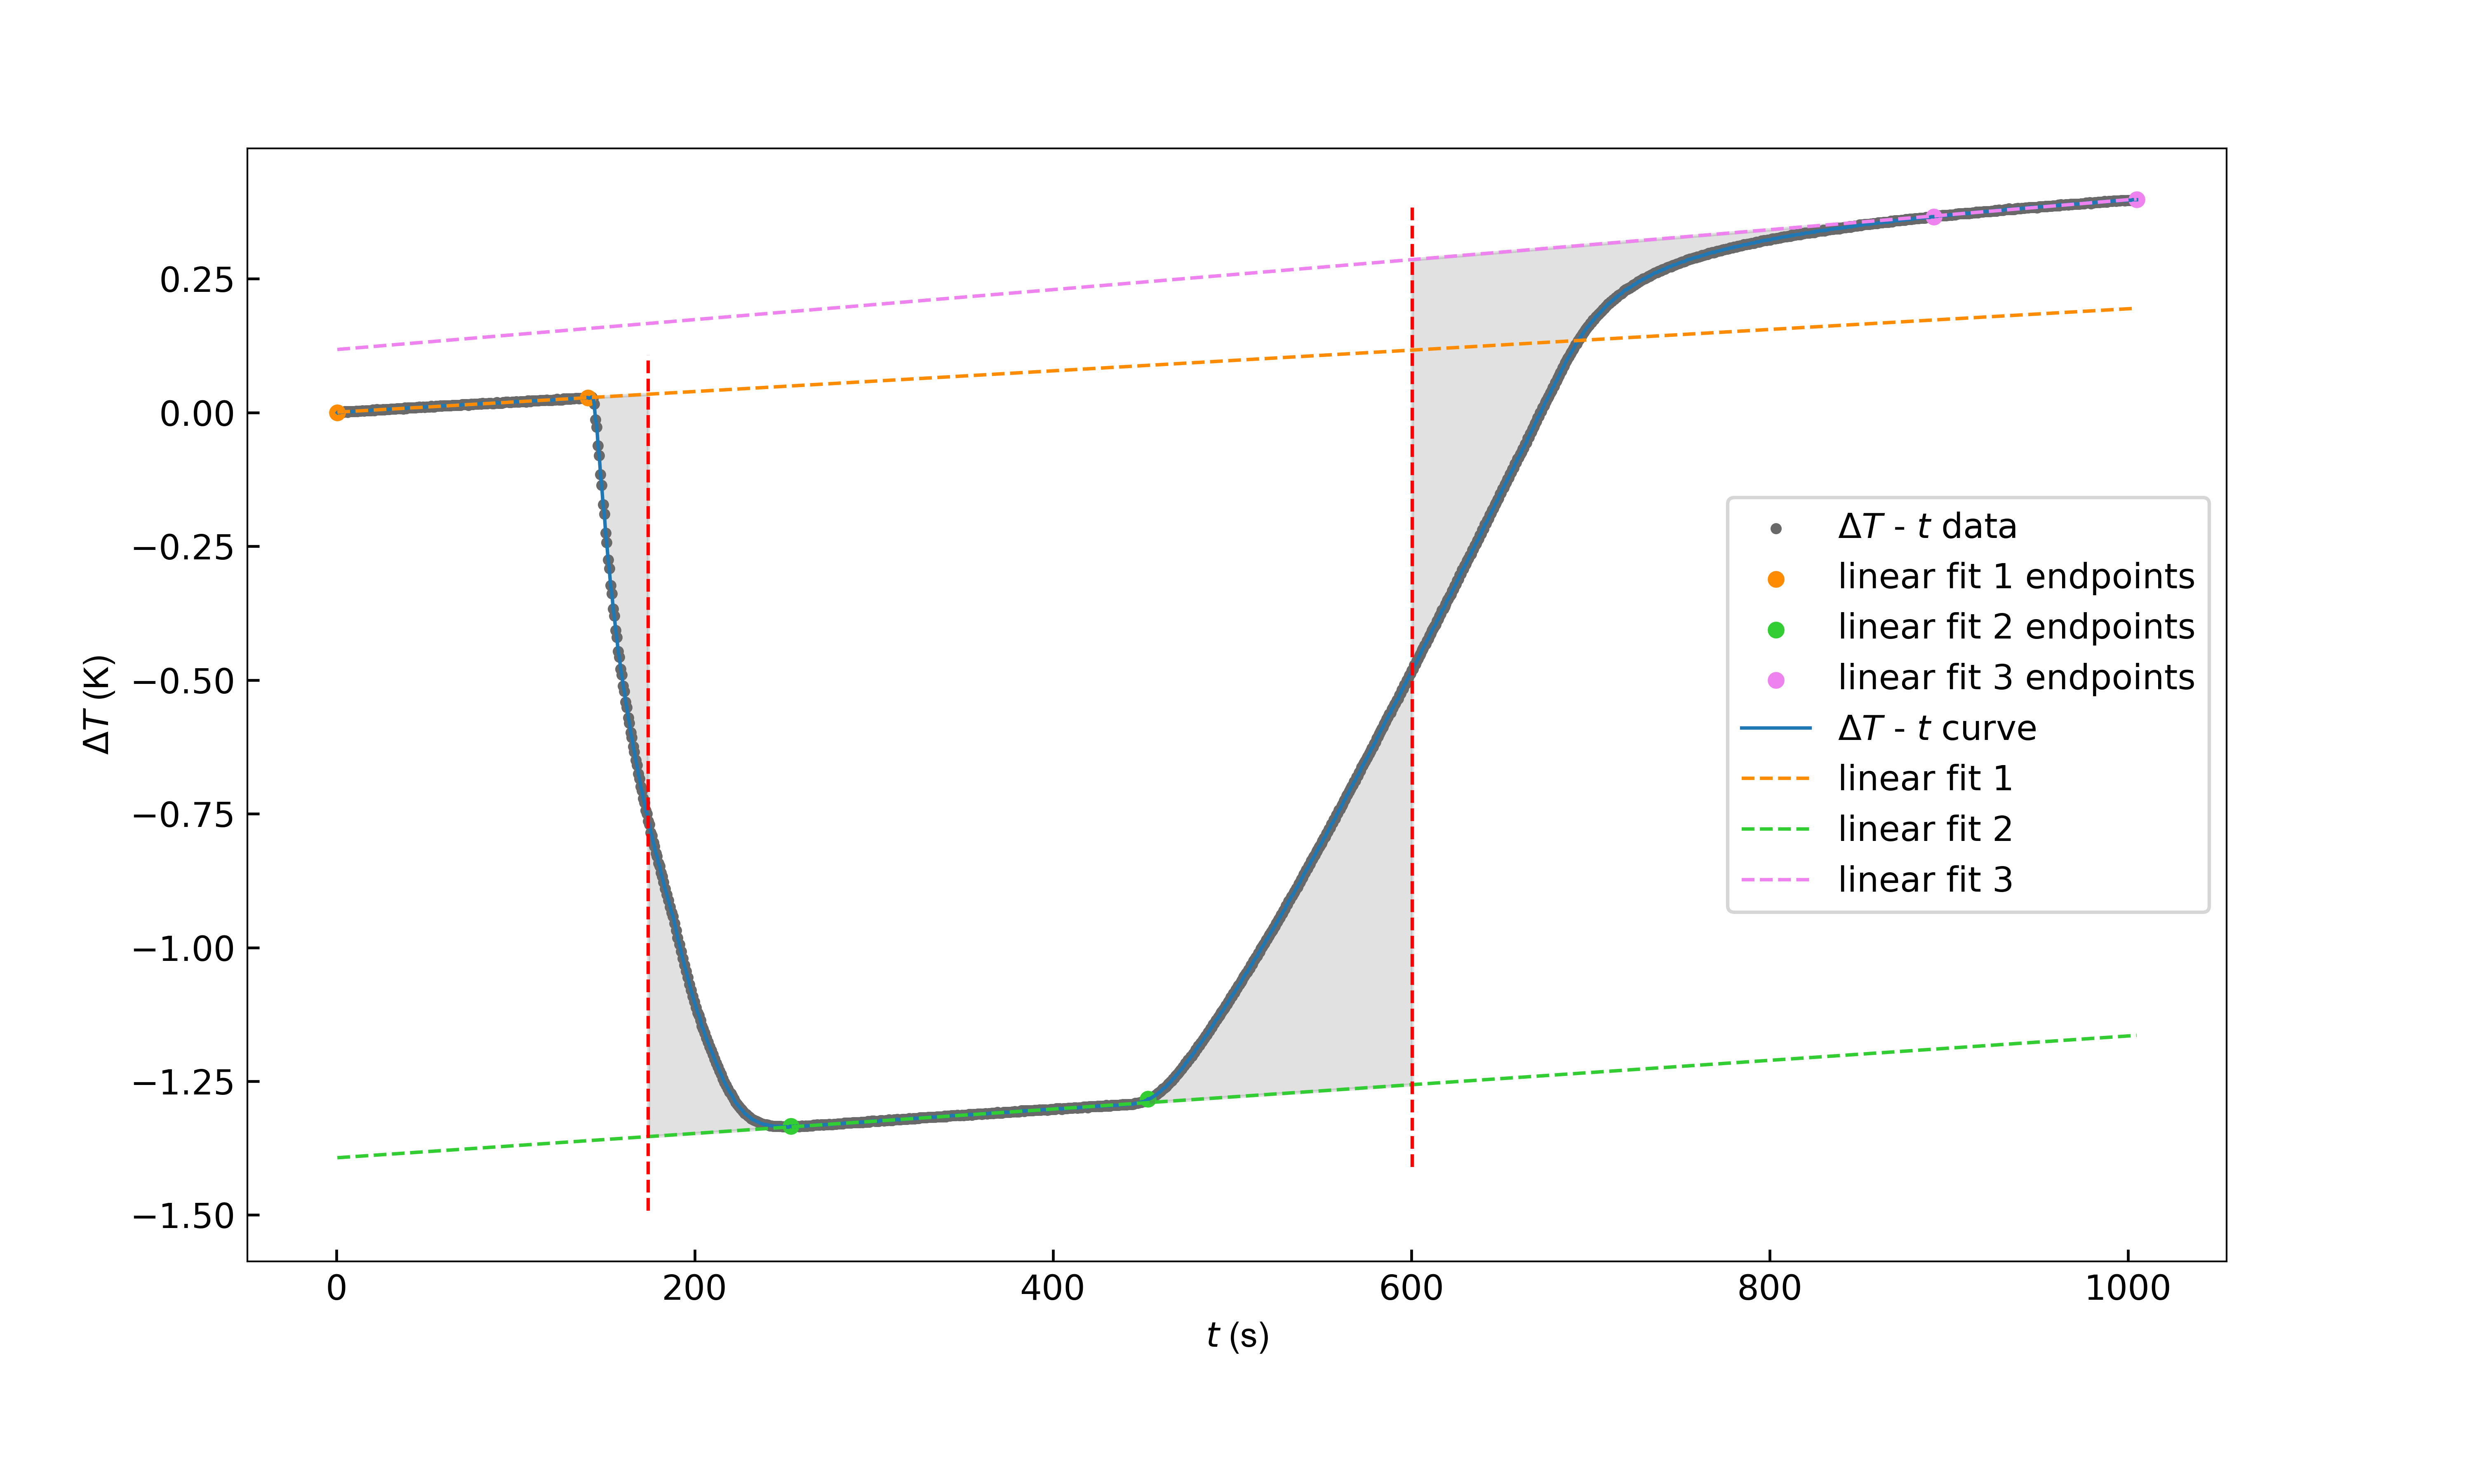
\includegraphics[width=\linewidth]{figures/3-5.png}
        \caption*{Loop2-5}
    \end{subfigure}
    \hfill
    \begin{subfigure}{0.45\textwidth}
        \centering
        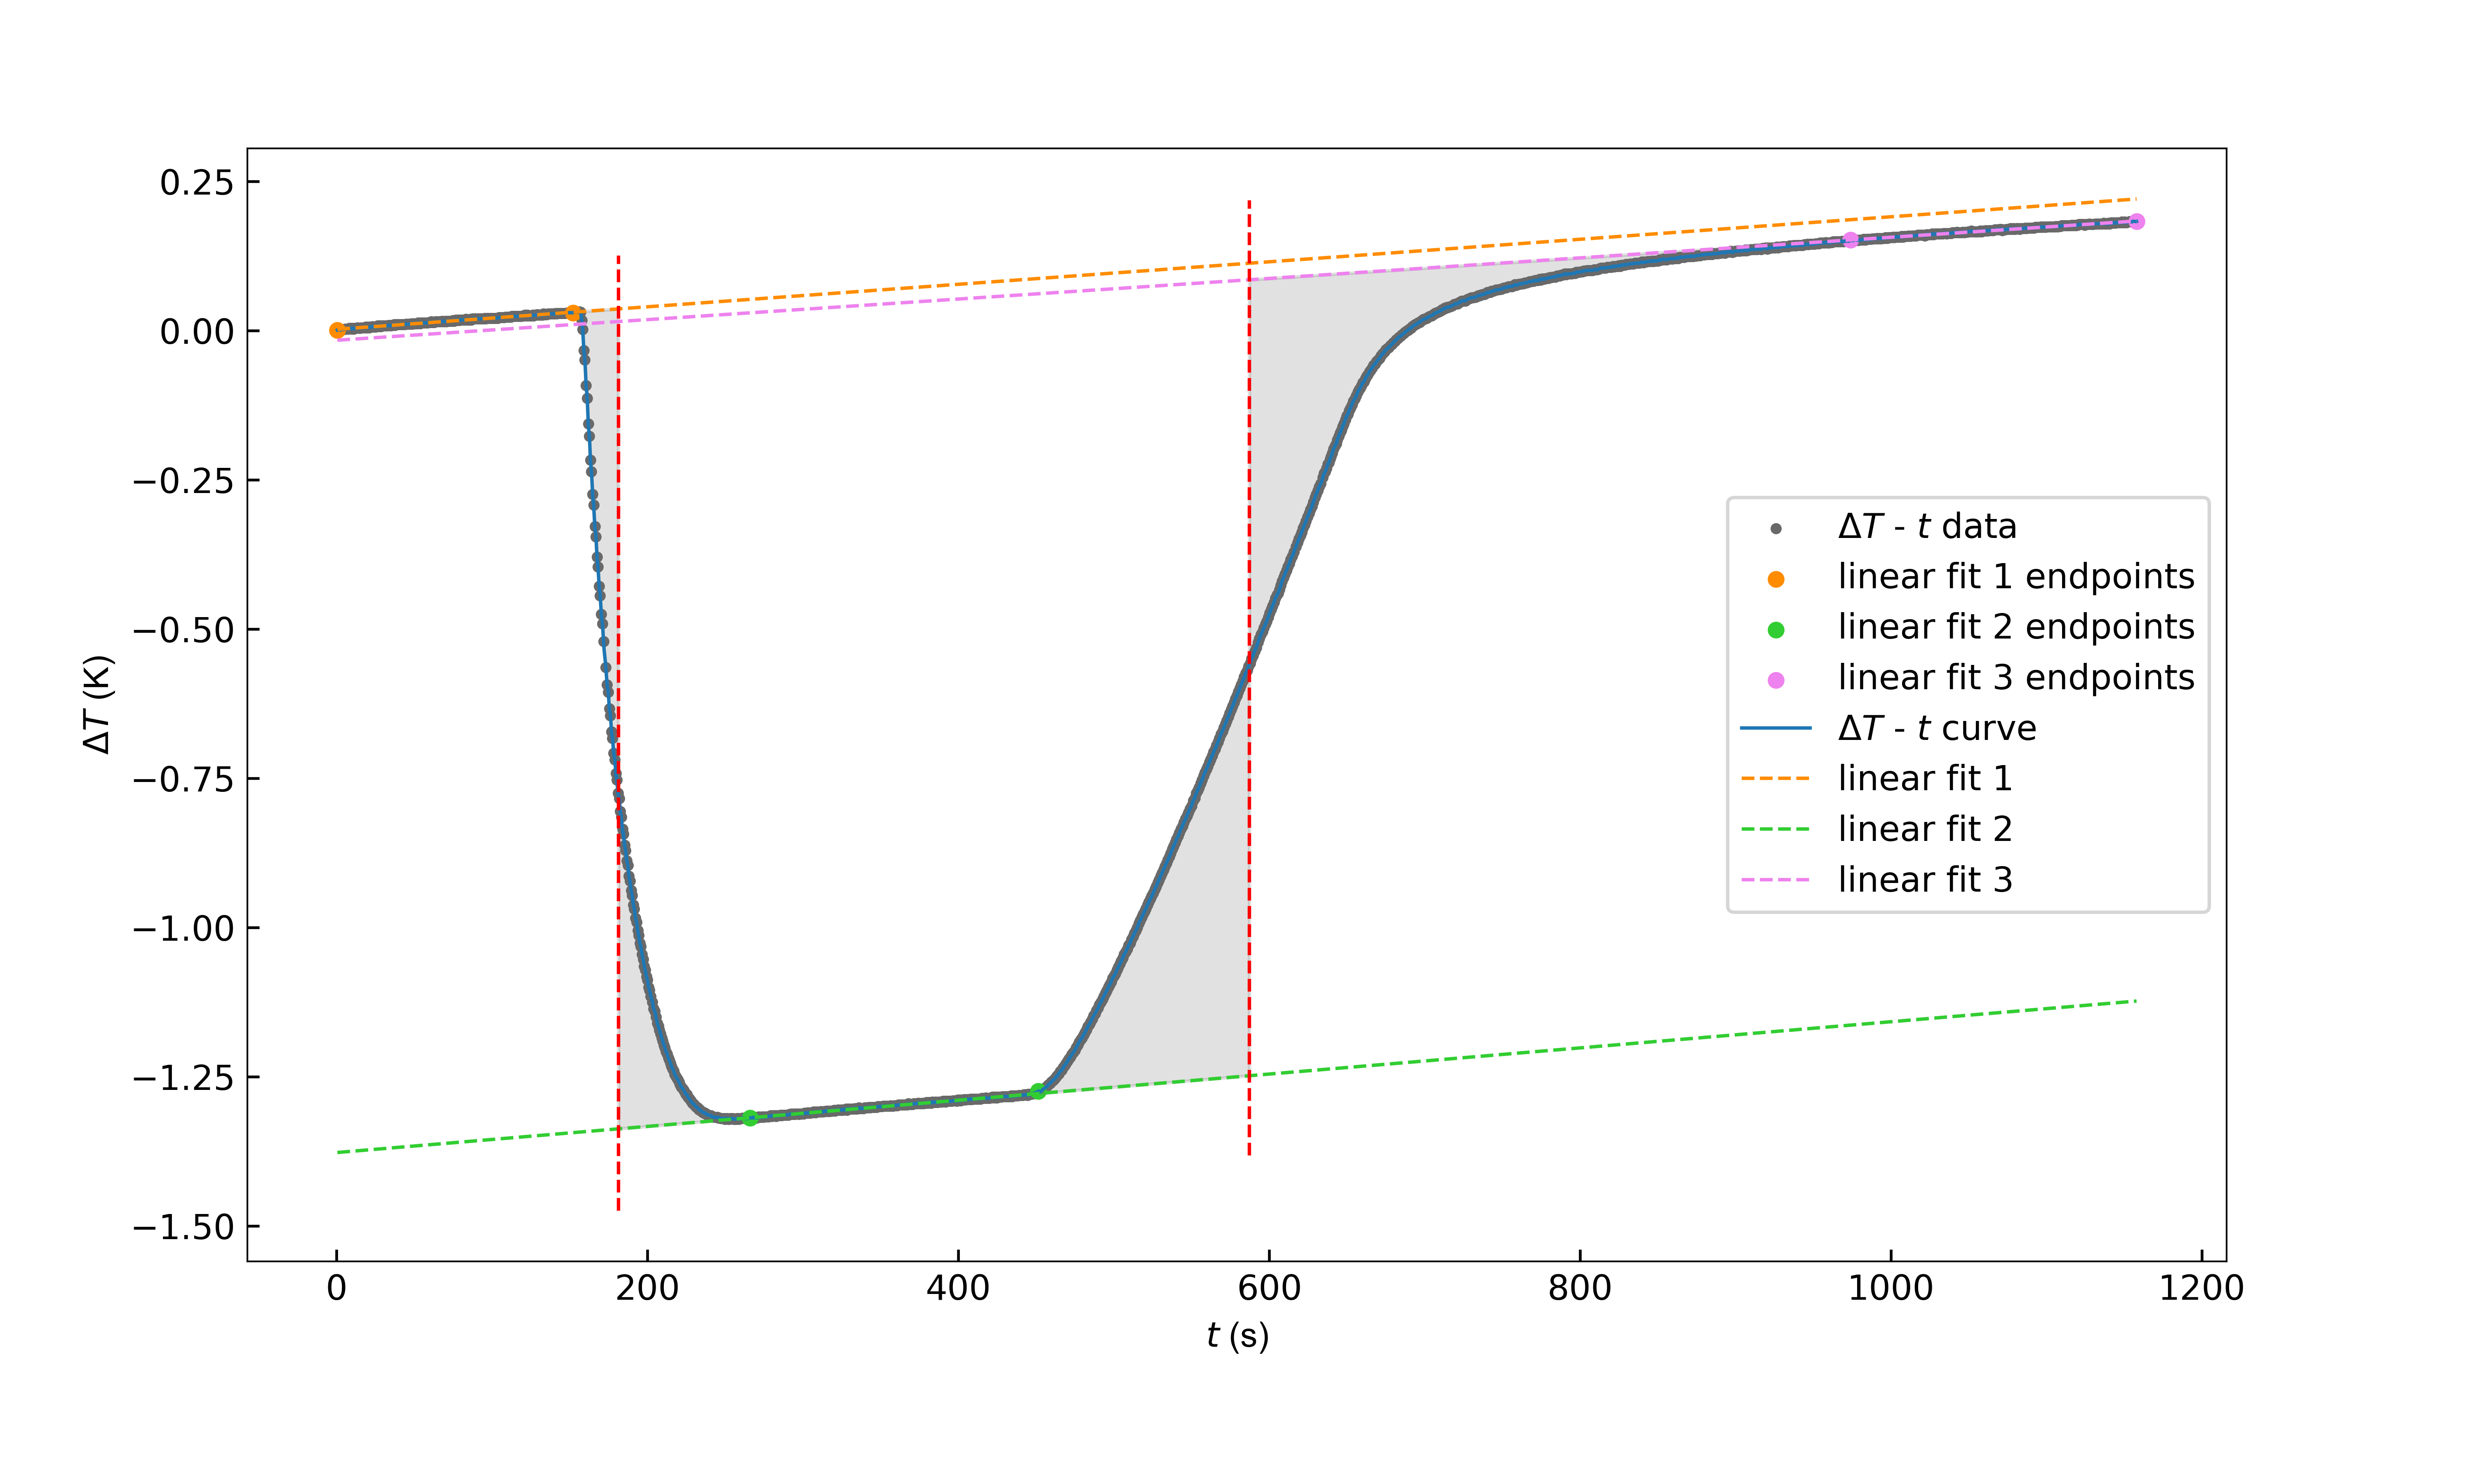
\includegraphics[width=\linewidth]{figures/3-6.png}
        \caption*{Loop2-6}
    \end{subfigure}
    \caption{第二轮实验的雷诺校正图}
    \label{fig:4}
\end{figure}

\begin{center}
    \begin{longtable}{cc}
        \midrule
        \endhead

        \caption{每次实验的三条拟合直线\label{tab:4}}\\
        \toprule
        实验序号-直线 & 拟合直线 \\
        \midrule
        \endfirsthead

        \midrule
        \endfoot

        \bottomrule
        \endlastfoot
        
        Loop1-1-Line1 & $\Delta T/\mathrm{~{}^\circ C} = (3.456\pm 0.125) \times 10^{-5}t/\mathrm{~s} + (1.069\pm 0.076) \times 10^{-3} \quad r^2 = 0.8390$ \\
        Loop1-1-Line2 & $\Delta T/\mathrm{~{}^\circ C} = (2.455\pm 0.053) \times 10^{-4}t/\mathrm{~s} + (-2.875\pm 0.0013) \quad r^2 = 0.9296$ \\
        Loop1-1-Line3 & $\Delta T/\mathrm{~{}^\circ C} = (1.725\pm 0.013) \times 10^{-4}t/\mathrm{~s} + (-0.0319\pm 0.0015) \quad r^2 = 0.9808$ \\
        Loop1-2-Line1 & $\Delta T/\mathrm{~{}^\circ C} = (7.441\pm 0.054) \times 10^{-5}t/\mathrm{~s} + (2.603\pm 5.710) \times 10^{-5} \quad r^2 = 0.9867$ \\
        Loop1-2-Line2 & $\Delta T/\mathrm{~{}^\circ C} = (2.395\pm 0.012) \times 10^{-4}t/\mathrm{~s} + (-2.677\pm 0.00044) \quad r^2 = 0.9919$ \\
        Loop1-2-Line3 & $\Delta T/\mathrm{~{}^\circ C} = (1.898\pm 0.010) \times 10^{-4}t/\mathrm{~s} + (-0.1129\pm 0.0012) \quad r^2 = 0.9928$ \\
        Loop1-3-Line1 & $\Delta T/\mathrm{~{}^\circ C} = (1.118\pm 0.007) \times 10^{-4}t/\mathrm{~s} + (1.548\pm 0.060) \times 10^{-3} \quad r^2 = 0.9922$ \\
        Loop1-3-Line2 & $\Delta T/\mathrm{~{}^\circ C} = (2.873\pm 0.051) \times 10^{-4}t/\mathrm{~s} + (-2.510\pm 0.001) \quad r^2 = 0.9526$ \\
        Loop1-3-Line3 & $\Delta T/\mathrm{~{}^\circ C} = (2.969\pm 0.019) \times 10^{-4}t/\mathrm{~s} + (-0.1268\pm 0.0016) \quad r^2 = 0.9941$ \\
        Loop1-4-Line1 & $\Delta T/\mathrm{~{}^\circ C} = (1.613\pm 0.007) \times 10^{-4}t/\mathrm{~s} + (1.719\pm 0.009) \times 10^{-2} \quad r^2 = 0.9941$ \\
        Loop1-4-Line2 & $\Delta T/\mathrm{~{}^\circ C} = (2.412\pm 0.024) \times 10^{-4}t/\mathrm{~s} + (-2.338\pm 0.001) \quad r^2 = 0.9772$ \\
        Loop1-4-Line3 & $\Delta T/\mathrm{~{}^\circ C} = (2.678\pm 0.020) \times 10^{-4}t/\mathrm{~s} + (0.5138\pm 0.0022)
        \quad r^2 = 0.9917$ \\
        \midrule
        Loop2-1-Line1 & $\Delta T/\mathrm{~{}^\circ C} = (6.858\pm 0.120) \times 10^{-5}t/\mathrm{~s} + (-2.048\pm 0.829) \times 10^{-4} \quad r^2 = 0.9513$ \\
        Loop2-1-Line2 & $\Delta T/\mathrm{~{}^\circ C} = (1.694\pm 0.021) \times 10^{-4}t/\mathrm{~s} + (-1.464\pm 0.0006) \quad r^2 = 0.9593$ \\
        Loop2-1-Line3 & $\Delta T/\mathrm{~{}^\circ C} = (2.623\pm 0.016) \times 10^{-4}t/\mathrm{~s} + (-0.0724\pm 0.0014) \quad r^2 = 0.9928$ \\
        Loop2-2-Line1 & $\Delta T/\mathrm{~{}^\circ C} = (1.651\pm 0.009) \times 10^{-4}t/\mathrm{~s} + (1.927\pm 0.069) \times 10^{-3} \quad r^2 = 0.9945$ \\
        Loop2-2-Line2 & $\Delta T/\mathrm{~{}^\circ C} = (2.269\pm 0.027) \times 10^{-4}t/\mathrm{~s} + (-1.441\pm 0.0009) \quad r^2 = 0.9688$ \\
        Loop2-2-Line3 & $\Delta T/\mathrm{~{}^\circ C} = (2.670\pm 0.015) \times 10^{-4}t/\mathrm{~s} + (-0.1102\pm 0.0014) \quad r^2 = 0.9926$ \\
        Loop2-3-Line1 & $\Delta T/\mathrm{~{}^\circ C} = (1.729\pm 0.009) \times 10^{-4}t/\mathrm{~s} + (5.273\pm 0.788) \times 10^{-4} \quad r^2 = 0.9945$ \\
        Loop2-3-Line2 & $\Delta T/\mathrm{~{}^\circ C} = (2.096\pm 0.010) \times 10^{-4}t/\mathrm{~s} + (-1.422\pm 0.0004) \quad r^2 = 0.9915$ \\
        Loop2-3-Line3 & $\Delta T/\mathrm{~{}^\circ C} = (3.175\pm 0.021) \times 10^{-4}t/\mathrm{~s} + (-0.1961\pm 0.0020) \quad r^2 = 0.9944$ \\
        Loop2-4-Line1 & $\Delta T/\mathrm{~{}^\circ C} = (1.869\pm 0.011) \times 10^{-4}t/\mathrm{~s} + (2.000\pm 0.075) \times 10^{-3} \quad r^2 = 0.9945$ \\
        Loop2-4-Line2 & $\Delta T/\mathrm{~{}^\circ C} = (2.211\pm 0.009) \times 10^{-4}t/\mathrm{~s} + (-1.404\pm 0.0003) \quad r^2 = 0.9959$ \\
        Loop2-4-Line3 & $\Delta T/\mathrm{~{}^\circ C} = (2.757\pm 0.015) \times 10^{-4}t/\mathrm{~s} + (-0.1288\pm 0.0014) \quad r^2 = 0.9945$ \\
        Loop2-5-Line1 & $\Delta T/\mathrm{~{}^\circ C} = (1.939\pm 0.010) \times 10^{-4}t/\mathrm{~s} + (7.304\pm 0.819) \times 10^{-4} \quad r^2 = 0.9956$ \\
        Loop2-5-Line2 & $\Delta T/\mathrm{~{}^\circ C} = (2.277\pm 0.009) \times 10^{-4}t/\mathrm{~s} + (-1.393\pm 0.0003) \quad r^2 = 0.9961$ \\
        Loop2-5-Line3 & $\Delta T/\mathrm{~{}^\circ C} = (2.801\pm 0.016) \times 10^{-4}t/\mathrm{~s} + 0.1178\pm 0.0015 \quad r^2 = 0.9948$ \\
        Loop2-6-Line1 & $\Delta T/\mathrm{~{}^\circ C} = (1.885\pm 0.008) \times 10^{-4}t/\mathrm{~s} + (2.149\pm 0.076) \times 10^{-3} \quad r^2 = 0.9955$ \\
        Loop2-6-Line2 & $\Delta T/\mathrm{~{}^\circ C} = (2.192\pm 0.007) \times 10^{-4}t/\mathrm{~s} + (-1.377\pm 0.0003) \quad r^2 = 0.9971$ \\
        Loop2-6-Line3 & $\Delta T/\mathrm{~{}^\circ C} = (1.725\pm 0.009) \times 10^{-4}t/\mathrm{~s} + (-0.0162\pm 0.0010) \quad r^2 = 0.9948$ \\
    \end{longtable}
\end{center}

\subsection{硝酸钾溶解热的计算}

本实验中,首先需要计算得到电热补偿的热量$Q^\prime$,据此结合表 \ref{tab:3} 中雷诺校正得到的温度差,计算得到每次加入\ce{KNO_3}时,体系所吸收的热量$Q$,最终计算得到每次加入\ce{KNO_3}后的积分溶解热$Q_{\rm s}$。将实验数据带入以下公式,得到表 \ref{tab:5}、表 \ref{tab:6}。
\begin{align*}
    &Q^\prime = I^2Rt\\
    &Q = Q^\prime\frac{T_2-T_1}{T_2^\prime-T_1^\prime}=I^2Rt\frac{\Delta T_a}{\Delta T_b}\\
    &Q_{\mathrm{s}} = \frac{\sum Q}{\sum n_2}
\end{align*}

\begin{table}[htbp]
    \centering
    \caption{补偿热$Q^\prime$的计算}
    \begin{tabular}{ccccccc}
    \toprule
    实验序号 & $t_1/\mathrm{S}$ & $t_2/\mathrm{S}$ & $\Delta t/\mathrm{S}$ & $R/\mathrm{\Omega}$ & $I/\mathrm{A}$ & $Q^\prime/\mathrm{J}$\\
    \midrule
    Loop1-1 & 286.057 & 932.651 & 646.594 & 11.3 & 0.97 & $6.87\times 10^{3}$\\
    Loop1-2 & 478.097 & 901.328 & 423.231 & 11.3 & 1.16 & $6.44\times 10^{3}$\\
    Loop1-3 & 309.730 & 575.890 & 266.160 & 11.3 & 1.46 & $6.41\times 10^{3}$\\
    Loop1-4 & 509.096 & 836.021 & 326.925 & 11.3 & 1.46 & $7.87\times 10^{3}$\\
    \midrule
    Loop2-1 & 366.245 & 592.694 & 226.449 & 11.3 & 1.26 & $4.06\times 10^{3}$\\
    Loop2-2 & 375.637 & 589.184 & 213.547 & 11.3 & 1.26 & $3.83\times 10^{3}$\\
    Loop2-3 & 509.279 & 714.157 & 204.878 & 11.3 & 1.26 & $3.68\times 10^{3}$\\
    Loop2-4 & 400.425 & 604.056 & 203.631 & 11.3 & 1.26 & $3.65\times 10^{3}$\\
    Loop2-5 & 437.183 & 675.979 & 238.796 & 11.3 & 1.26 & $4.28\times 10^{3}$\\
    Loop2-6 & 438.013 & 640.040 & 202.027 & 11.3 & 1.26 & $3.62\times 10^{3}$\\
    \bottomrule
    \end{tabular}
    \label{tab:5}
\end{table}

\begin{table}[htbp]
    \centering
    \caption{\ce{KNO_3}溶解热的计算}
    \begin{tabular}{ccccccccc}
        \toprule
        实验序号 & $\Delta T_a/\mathrm{{}^\circ C}$ & $\Delta T_b/\mathrm{{}^\circ C}$ & $Q^\prime/\mathrm{J}$ & $Q/\mathrm{J}$ & $\sum n_2/\mathrm{mol}$ & $Q_{\rm{s}}/\mathrm{J\cdot mol^{-1}}$ \\
        \midrule
        Loop1-1 & 2.849 & 2.795 & $6.87\times 10^{3}$ & $7.00\times 10^{3}$ & 0.1781 & $3.93\times 10^{4}$ \\
        Loop1-2 & 2.644 & 2.528 & $6.44\times 10^{3}$ & $6.74\times 10^{3}$ & 0.3561 & $3.86\times 10^{4}$ \\
        Loop1-3 & 2.482 & 2.387 & $6.41\times 10^{3}$ & $6.67\times 10^{3}$ & 0.5342 & $3.82\times 10^{4}$ \\
        Loop1-4 & 2.336 & 2.871 & $7.87\times 10^{3}$ & $6.40\times 10^{3}$ & 0.7122 & $3.76\times 10^{4}$ \\
        \midrule
        Loop2-1 & 1.449 & 1.440 & $4.06\times 10^{3}$ & $4.09\times 10^{3}$ & 0.08907 & $4.59\times 10^{4}$ \\
        Loop2-2 & 1.433 & 1.352 & $3.83\times 10^{3}$ & $4.06\times 10^{3}$ & 0.1806 & $4.49\times 10^{4}$ \\
        Loop2-3 & 1.416 & 1.297 & $3.68\times 10^{3}$ & $4.02\times 10^{3}$ & 0.2746 & $4.42\times 10^{4}$ \\
        Loop2-4 & 1.401 & 1.305 & $3.65\times 10^{3}$ & $3.92\times 10^{3}$ & 0.3711 & $4.33\times 10^{4}$ \\
        Loop2-5 & 1.387 & 1.542 & $4.28\times 10^{3}$ & $3.85\times 10^{3}$ & 0.4700 & $4.24\times 10^{4}$ \\
        Loop2-6 & 1.373 & 1.333 & $3.62\times 10^{3}$ & $3.73\times 10^{3}$ & 0.5714 & $4.14\times 10^{4}$ \\
        \bottomrule
    \end{tabular}
    \label{tab:6}
\end{table}

\subsection{积分溶解热与溶液浓度的关系}

\subsubsection{积分溶解热-溶液浓度倒数图的绘制}

对于第二轮实验的数据,绘制积分溶解热与溶液浓度倒数的关系图,即$Q_{\mathrm{s}}-n_0^{-1}$图 \ref{fig:5},其数据如表 \ref{tab:7}。

\begin{table}[htbp]
    \centering
    \caption{积分溶解热与溶液浓度的关系}
    \begin{tabular}{cccc}
        \toprule
        实验序号 & $n_0$ & $n_0^{-1}$ & $Q_{\mathrm{s}}$ \\
        \midrule
        1 & 311.57 & 0.0032096 & $4.59\times 10^{4}$ \\
        2 & 153.65 & 0.0065083 & $4.49\times 10^{4}$ \\
        3 & 101.07 & 0.0098941 & $4.42\times 10^{4}$ \\
        4 & 74.797 & 0.013370 & $4.33\times 10^{4}$ \\
        5 & 59.045 & 0.016936 & $4.24\times 10^{4}$ \\
        6 & 48.568 & 0.020590 & $4.14\times 10^{4}$ \\
        \bottomrule
    \end{tabular}
    \label{tab:7}
\end{table}

\begin{figure}[htbp]
    \centering
    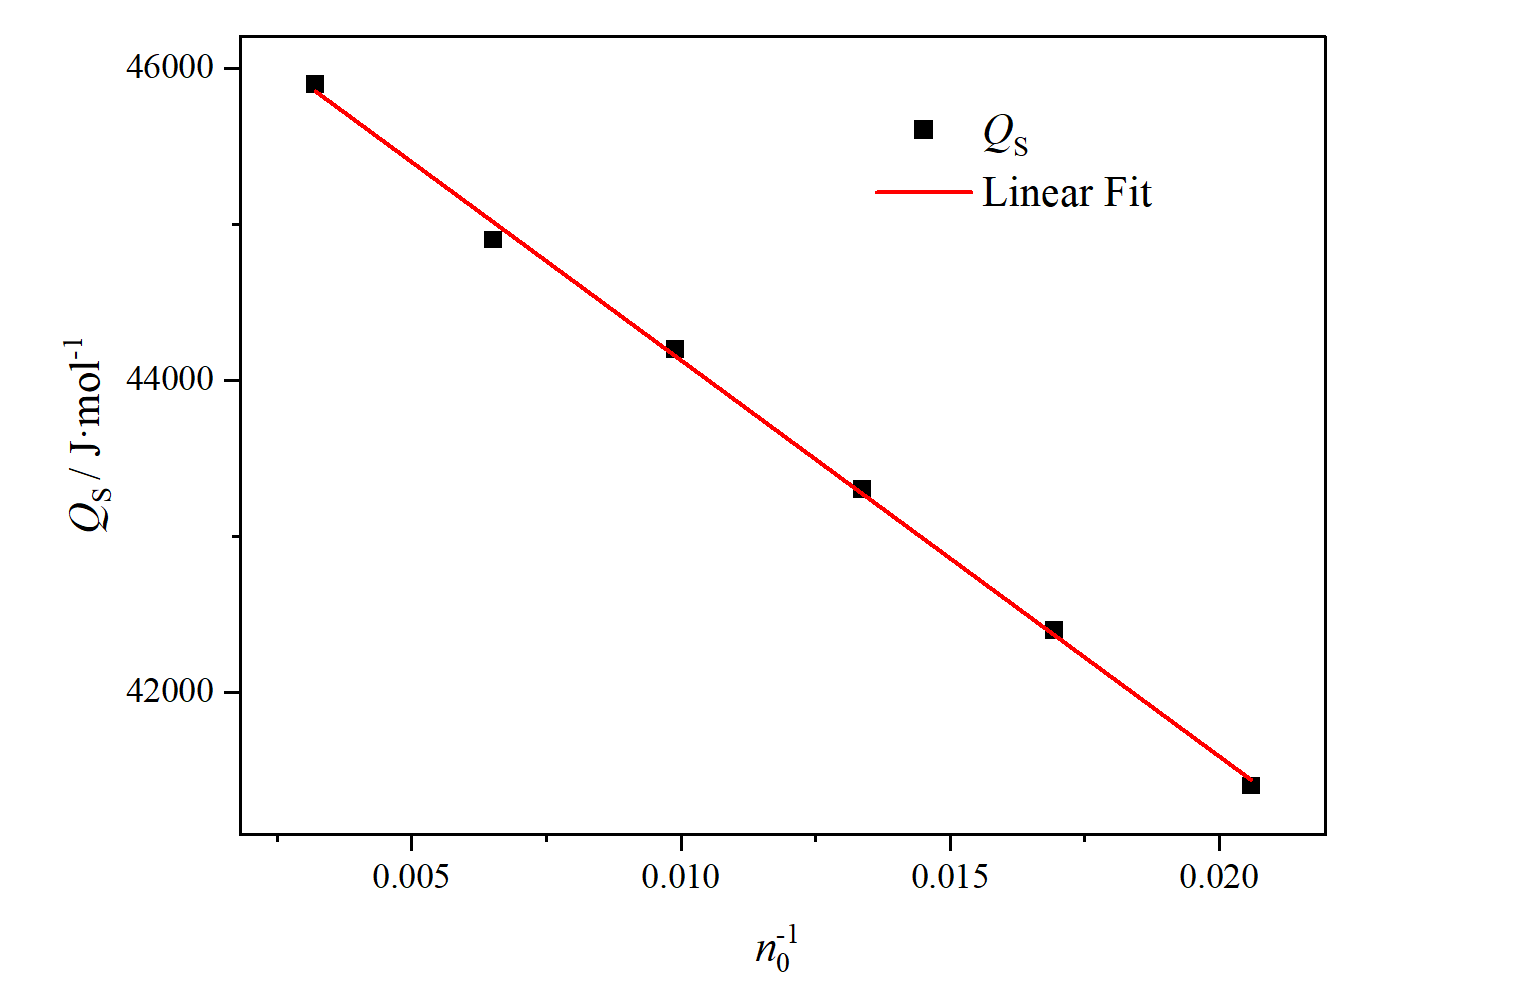
\includegraphics[width=.75\textwidth]{figures/4-1.png}
    \caption{$Q_{\mathrm{s}}-n_0^{-1}$图与拟合直线}
    \label{fig:5}
\end{figure}

\subsubsection{Origin 作图求算溶解吸热}

我们选取第二轮实验的最后一组数据(Loop2-6)进行分析,首先,对于三段平台期进行线性拟合,得到的结果如图 \ref{fig:5a},拟合直线表达式如表 \ref{tab:8}。

\begin{figure}[htbp]
    \centering
    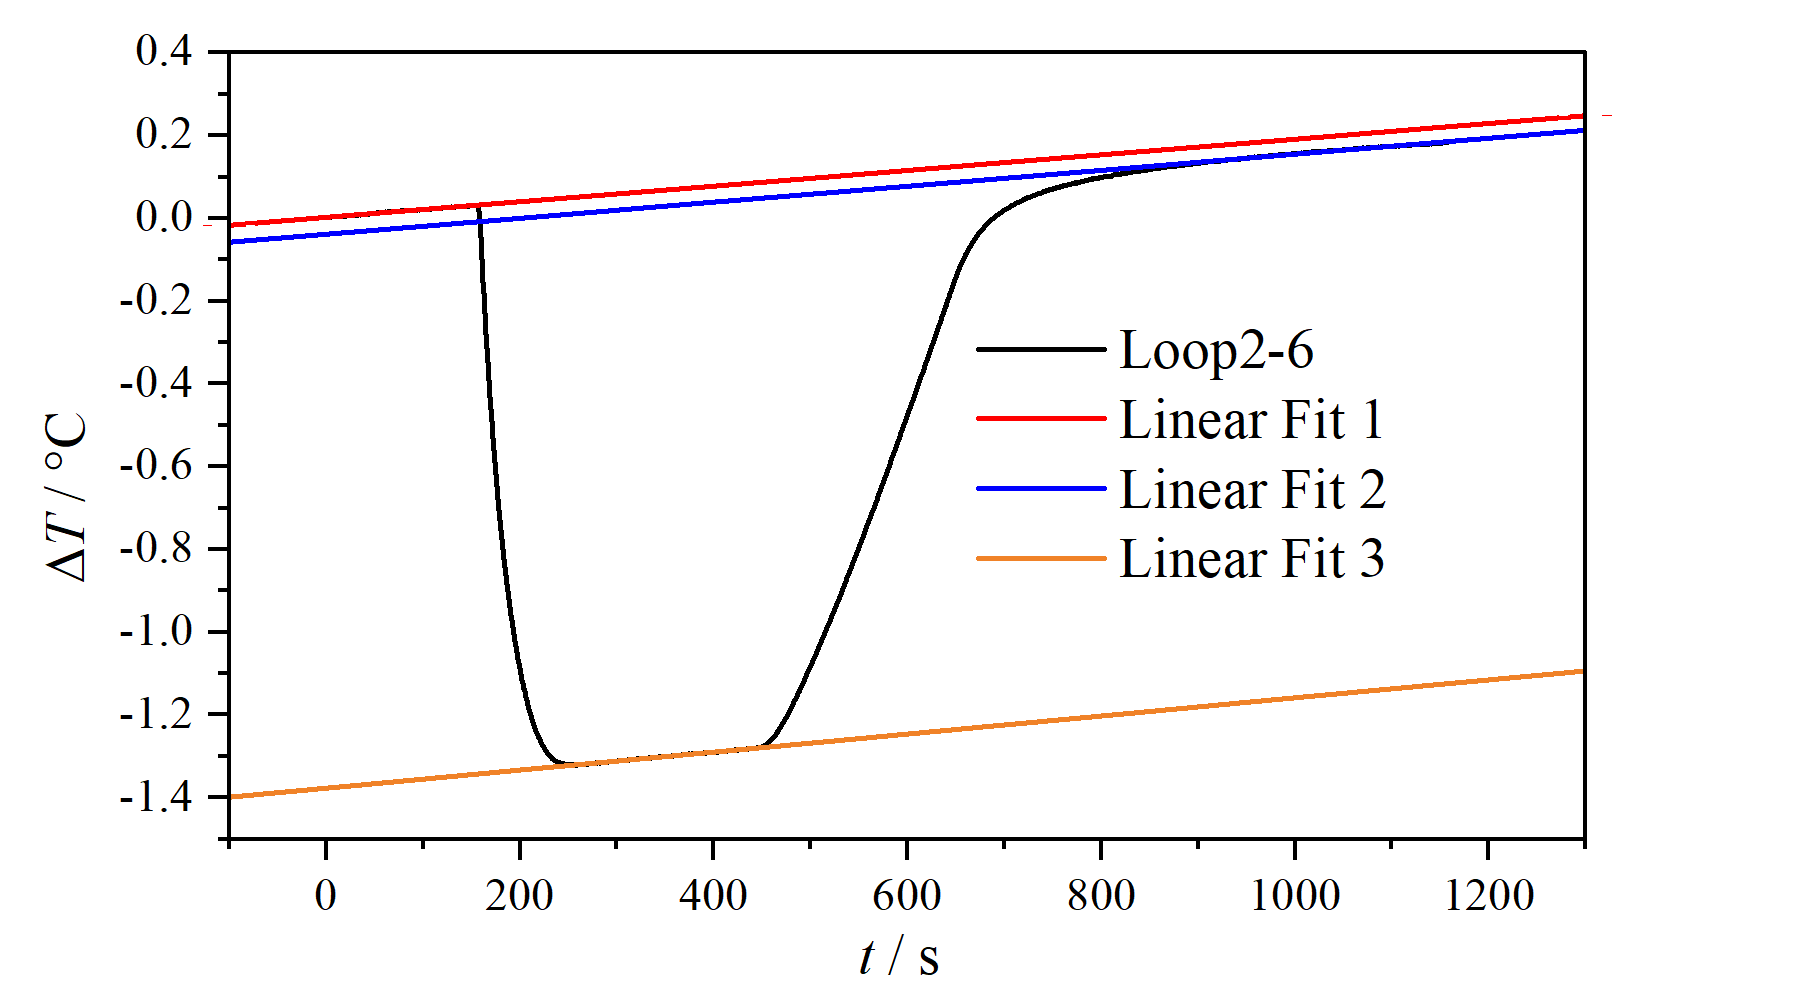
\includegraphics[width=.75\textwidth]{figures/4-2.png}
    \caption{Loop2-6的温度-时间关系图}
    \label{fig:5a}
\end{figure}

\begin{table}[htbp]
    \centering
    \caption{Loop2-6的拟合直线}
    \begin{tabular}{cc}
        \toprule
         实验序号-直线 & 拟合直线 \\
         \midrule
         Loop2-6-Line1 & $\Delta T/\mathrm{~{}^\circ C} = (1.888\pm 0.001) \times 10^{-4}t/\mathrm{~s} + (0.00213\pm 0.00008) \quad r^2 = 0.99547$ \\
        Loop2-6-Line2 & $\Delta T/\mathrm{~{}^\circ C} = (1.935\pm 0.001) \times 10^{-4}t/\mathrm{~s} + (-0.03881\pm 0.0011) \quad r^2 = 0.99134$ \\
        Loop2-6-Line3 & $\Delta T/\mathrm{~{}^\circ C} = (2.179\pm 0.001) \times 10^{-4}t/\mathrm{~s} + (-1.37659\pm 0.00023) \quad r^2 = 0.99777$ \\
        \bottomrule
    \end{tabular}
    \label{tab:8}
\end{table}

根据表 \ref{tab:8}可以发现,三段平台期由于磁子搅拌,均有着相近的斜率,即升温速率,记为$k_1,k_2,k_3$。为了消除升温速率对于温度差带来的影响,对于溶解降温和加热升温两个过程,分别选取相邻两段拟合直线斜率的平均值$k_a, k_b$,作为升降温过程中,体系自身的温度变化速率:
\begin{align*}
    k_a &= \frac{k_1+k_2}{2} = 1.912\times 10^{-4}\\
    k_b &= \frac{k_2+k_3}{2} = 2.057\times 10^{-4}
\end{align*}

选取降温与升温过程的起止温度$T_1,T_2,T_2^\prime,T_1^\prime$及其对应的时间$t_1,t_2,t_2^\prime,t_1^\prime$,如表 \ref{tab:9}。
\begin{table}[htbp]
    \centering
    \caption{Loop2-6中升降温的起止温度及其对应时间}
    \begin{tabular}{cccccccc}
        \toprule
         $T_1$ & $t_1$ & $T_2$ & $t_2$ & $T_2^\prime$ & $t_2^\prime$ & $T_1^\prime$ & $t_1^\prime$\\
         \midrule
         0.032 & 166.278 & -1.321 & 249.831 & -1.279 & 447.251 & 0.126 & 875.315\\
         \bottomrule         
    \end{tabular}
    \label{tab:9}
\end{table}

进一步,求出温度差$\Delta T_a,\Delta T_b$与时间差$\Delta t_a,\Delta t_b$,如表 \ref{tab:9a}。
\begin{table}[htbp]
    \centering
    \caption{Loop2-6中升降温的起止温度及其对应时间}
    \begin{tabular}{cccc}
        \toprule
         $\Delta T_a$ & $\Delta t_a$ & $\Delta T_b$ & $\Delta t_b$ \\
         \midrule
         1.353 & 83.553 & 1.399 & 428.064 \\
         \bottomrule         
    \end{tabular}
    \label{tab:9a}
\end{table}

使用$k_a,k_b$对于温度差进行校正:
\begin{align*}
    \Delta T_a^\prime &= \Delta T_a + k_a\Delta t_a = 1.369 \mathrm{~{}^\circ C}\\
    \Delta T_b^\prime &= \Delta T_b - k_b\Delta t_b = 1.310 \mathrm{~{}^\circ C}
\end{align*}

根据表 \ref{tab:5} 可知,Loop2-6中的补偿热 $Q^\prime = 3.62\times 10^{3} \mathrm{~J}$,据此,可以求得\ce{KNO_3}的溶解热:
\begin{equation*}
    Q = Q^\prime \times \frac{\Delta T_a^\prime}{\Delta T_b^\prime} = 3.78 \times 10^{3} \mathrm{~J}
\end{equation*}

这与表 \ref{tab:5} 中使用雷诺校正得到的结果 $Q = 3.73 \times 10^{3} \mathrm{~J}$ 非常接近,可以认为使用平均斜率的校正方法可靠。

\section{结果与讨论}
\subsection{误差分析}

由于第一轮实验的内容与第二轮几乎完全相同,其误差分析也一致,为了方便起见,我们使用第二轮实验的数据进行误差分析。出于书写方便考虑,在表示误差$\sigma$时,将会略去单位,其单位与其对应的测量值保持一致。

\subsubsection{雷诺校正后的温度不确定度计算}

首先,要求计算温度的不确定度。而温度的不确定度主要由两部分构成:温度传感器自身的不确定度、拟合直线中预测值的不确定度。其中,我们假定温度传感器自身的不确定度为其示数最后一位的数量级的一半,即:
\begin{equation}\label{eq:3}
    \sigma_{T} = \frac{10^{-4}}{2} = 5\times10^{-5}
\end{equation}

接下来,计算拟合直线的预测值(温度$T_1,T_2,T_2^\prime,T_1^\prime$)的不确定度。

在最小二乘法进行的线性回归中$y = ax + b + \varepsilon$,预测值$\hat y$的标准误差可以表示为
\begin{equation*}
    \sigma_{\hat{y}} = \sqrt{ \sigma_{a}^2 \cdot x^2 + \sigma_{b}^2 + 2 \cdot \mathrm{Cov}(a, b) \cdot x + \sigma^2 } 
\end{equation*}
其中,协方差$\mathrm{Cov}(a,b)$与残差$\sigma^2$一般较小,可以忽略,因此,我们得到
\begin{equation}\label{eq:2}
    \sigma_{\hat{y}} = \sqrt{ \sigma_{a}^2 \cdot x^2 + \sigma_{b}^2}
\end{equation}
根据表 \ref{tab:3} 与表 \ref{tab:4} ,带入式 \eqref{eq:2} 中得到表 \ref{tab:10}。

\begin{table}[htbp]
    \centering
    \caption{拟合直线预测值的不确定度}
    \begin{tabular}{ccccc}
        \toprule
        实验序号 & $\sigma_{T_1}^\prime$ & $\sigma_{T_2}^\prime$ & $\sigma_{T_2^\prime}^\prime$ & $\sigma_{T_1^\prime}^\prime$ \\
        \midrule
        1 & $1.92 \times 10^{-4}$ & $6.72 \times 10^{-4}$ & $1.25 \times 10^{-3}$ & $1.63 \times 10^{-3}$ \\
        2 & $1.59 \times 10^{-4}$ & $9.97 \times 10^{-4}$ & $1.68 \times 10^{-3}$ & $1.61 \times 10^{-3}$ \\
        3 & $1.72 \times 10^{-4}$ & $4.35 \times 10^{-4}$ & $7.67 \times 10^{-4}$ & $2.43 \times 10^{-3}$ \\
        4 & $1.81 \times 10^{-4}$ & $3.29 \times 10^{-4}$ & $5.76 \times 10^{-4}$ & $1.62 \times 10^{-3}$ \\
        5 & $1.92 \times 10^{-4}$ & $3.38 \times 10^{-4}$ & $6.18 \times 10^{-4}$ & $1.78 \times 10^{-3}$ \\
        6 & $1.64 \times 10^{-4}$ & $3.26 \times 10^{-4}$ & $5.09 \times 10^{-4}$ & $1.13 \times 10^{-3}$ \\
        \bottomrule
    \end{tabular}
    \label{tab:10}
\end{table}

根据误差传递公式:
\begin{equation}\label{eq:4}
    \sigma_{\Delta T}= \sqrt{\sigma_{T_1}^2+\sigma_{T_2}^2}
\end{equation}
将表 \ref{tab:10} 中的数据与仪器自身的不确定度 \eqref{eq:3} 带入式 \eqref{eq:4} 得到温度的不确定度如表 \ref{tab:11}。

\begin{table}[htbp]
    \centering
    \caption{拟合直线预测值的不确定度}
    \begin{tabular}{ccccc}
        \toprule
        实验序号 & $\sigma_{T_1}^\prime$ & $\sigma_{T_2}^\prime$ & $\sigma_{T_2^\prime}^\prime$ & $\sigma_{T_1^\prime}^\prime$ \\
        \midrule
        1 & $1.98 \times 10^{-4}$ & $6.74 \times 10^{-4}$ & $1.25 \times 10^{-3}$ & $1.63 \times 10^{-3}$ \\
        2 & $1.67 \times 10^{-4}$ & $9.98 \times 10^{-4}$ & $1.68 \times 10^{-3}$ & $1.61 \times 10^{-3}$ \\
        3 & $1.79 \times 10^{-4}$ & $4.38 \times 10^{-4}$ & $7.69 \times 10^{-4}$ & $2.43 \times 10^{-3}$ \\
        4 & $1.87 \times 10^{-4}$ & $3.32 \times 10^{-4}$ & $5.78 \times 10^{-4}$ & $1.62 \times 10^{-3}$ \\
        5 & $1.99 \times 10^{-4}$ & $3.42 \times 10^{-4}$ & $6.20 \times 10^{-4}$ & $1.78 \times 10^{-3}$ \\
        6 & $1.71 \times 10^{-4}$ & $3.30 \times 10^{-4}$ & $5.11 \times 10^{-4}$ & $1.13 \times 10^{-3}$ \\
        \bottomrule
    \end{tabular}
    \label{tab:11}
\end{table}

最终,根据式 \eqref{eq:4},结合表 \ref{tab:3},得到温度差的不确定度如表 \ref{tab:12}。

\begin{table}[htbp]
    \centering
    \caption{温度差及其不确定度}
    \begin{tabular}{ccc}
        \toprule
        实验序号 & $\Delta T_a/\mathrm{{}^\circ C}$ & $\Delta T_b/\mathrm{{}^\circ C}$ \\
        \midrule
        1 & 1.449 $\pm$ 0.000702 & 1.440 $\pm$ 0.00206 \\
        2 & 1.433 $\pm$ 0.00101 & 1.352 $\pm$ 0.00233 \\
        3 & 1.416 $\pm$ 0.000473 & 1.297 $\pm$ 0.00255 \\
        4 & 1.401 $\pm$ 0.000382 & 1.305 $\pm$ 0.00172 \\
        5 & 1.387 $\pm$ 0.000396 & 1.542 $\pm$ 0.00189 \\
        6 & 1.373 $\pm$ 0.000371 & 1.333 $\pm$ 0.00124 \\
        \bottomrule
    \end{tabular}
    \label{tab:12}
\end{table}

\subsubsection{溶解热的不确定度计算}

首先,要计算出补偿热的不缺定度。根据补偿热的计算公式:
\begin{equation}
    Q^\prime = I^2R\Delta t
\end{equation}

其中,假定电流与电阻的误差分别为其有效数字最后一位的一半:
\begin{align*}
    \sigma_I &= \frac{1\times 10^{-2}}{2} = 5\times 10^{-3}\\
    \sigma_R &= \frac{1\times 10^{-1}}{2} = 5\times 10^{-2}
\end{align*}
而时间由于是自变量,不考虑其误差。

以第二轮实验的第一次为例,推导补偿热及其不确定度的计算:
\begin{equation*}
Q^\prime=R \Delta t I^{2}=\left(11.3\right) \times \left(226.449\right) \times \left(1.26\right)^{2}=4062.0\ \mathrm{~J}
\end{equation*}
\begin{equation*}
\begin{aligned}
\frac{\partial Q^\prime }{\partial I }&=2 R \Delta t I=2 \times \left(11.3\right) \times \left(226.449\right) \times \left(1.26\right)=6.4 \times 10^{3}\\
\frac{\partial Q^\prime }{\partial R }&=\Delta t I^{2}=\left(226.449\right) \times \left(1.26\right)^{2}=3.6 \times 10^{2}\\
\end{aligned}
\end{equation*}
\begin{equation*}
\begin{aligned}
\sigma_{Q^\prime}&=\sqrt{\left(\frac{\partial Q^\prime }{\partial I } \sigma_{I}\right)^2+\left(\frac{\partial Q^\prime }{\partial R } \sigma_{R}\right)^2}\\
&=\sqrt{\left(6.4 \times 10^{3} \times 0.005\right)^2+\left(3.6 \times 10^{2} \times 0.05\right)^2}\\
&=\sqrt{\left(32.0\right)^2+\left(18.0\right)^2}\\
&=37.0\ \mathrm{~J}
\end{aligned}
\end{equation*}
\begin{equation*}
Q^\prime=\left (4062 \pm 37 \right )\ \mathrm{~J}
\end{equation*}

进一步地,求溶解热及其不确定度的计算。根据溶解热的计算公式:
\begin{equation*}
    Q = Q^\prime \frac{\Delta T_a}{\Delta T_b}
\end{equation*}

根据表 \ref{tab:12},有:
\begin{equation*}
Q=\frac{Q^\prime \Delta T_a}{\Delta T_b}=\frac{\left(4062.0\right) \times \left(1.449\right)}{\left(1.44\right)}=4087.0\ \mathrm{~J}
\end{equation*}
\begin{equation*}
\begin{aligned}
\frac{\partial Q }{\partial Q^\prime }&=\frac{\Delta T_a}{\Delta T_b}=\frac{\left(1.449\right)}{\left(1.44\right)}=1.0\\
\frac{\partial Q }{\partial \Delta T_a }&=\frac{Q^\prime}{\Delta T_b}=\frac{\left(4062.0\right)}{\left(1.44\right)}=2.8 \times 10^{3}\\
\frac{\partial Q }{\partial \Delta T_b }&=- \frac{Q^\prime \Delta T_a}{\Delta T_b^{2}}=- \frac{\left(4062.0\right) \times \left(1.449\right)}{\left(1.44\right)^{2}}=-2.8 \times 10^{3}\\
\end{aligned}
\end{equation*}
\begin{equation*}
\begin{aligned}
\sigma_{Q}&=\sqrt{\left(\frac{\partial Q }{\partial Q^\prime } \sigma_{Q^\prime}\right)^2+\left(\frac{\partial Q }{\partial \Delta T_a } \sigma_{\Delta T_a}\right)^2+\left(\frac{\partial Q }{\partial \Delta T_b } \sigma_{\Delta T_b}\right)^2}\\
&=\sqrt{\left(1.0 \times 37.0\right)^2+\left(2.8 \times 10^{3} \times 0.0007\right)^2+\left(-2.8 \times 10^{3} \times 0.0021\right)^2}\\
&=\sqrt{\left(37.0\right)^2+\left(2.0\right)^2+\left(-5.8\right)^2}\\
&=38.0\ \mathrm{~J}
\end{aligned}
\end{equation*}
\begin{equation*}
Q=\left (4087 \pm 38 \right )\ \mathrm{~J}
\end{equation*}
类似地,我们可以得到每次实验补偿热、溶解热及其各自的不确定度,如表 \ref{tab:13}。

\begin{table}[htbp]
    \centering
    \caption{补偿热、溶解热及其各自不确定度}
    \begin{tabular}{ccc}
        \toprule
        实验序号 & $Q^\prime/\mathrm{J}$ & $Q/\mathrm{J}$ \\
        \midrule
        1 & 4062 $\pm$ 37 & 4087 $\pm$ 38 \\
        2 & 3831 $\pm$ 35 & 4061 $\pm$ 38 \\
        3 & 3676 $\pm$ 33 & 4033 $\pm$ 37 \\
        4 & 3653 $\pm$ 33 & 3922 $\pm$ 36 \\
        5 & 4284 $\pm$ 39 & 3853 $\pm$ 35 \\
        6 & 3624 $\pm$ 33 & 3733 $\pm$ 34 \\
        \bottomrule
    \end{tabular}
    \label{tab:13}
\end{table}

\subsubsection{积分溶解热的不确定度计算}\label{sec:1}

根据积分溶解热的计算公式:
\begin{equation}\label{eq:5}
    Q_{\mathrm{s}} = \frac{\sum Q}{\sum n_2} = \frac{M_{\ce{KNO_3}}\sum Q}{\sum m_{\ce{KNO_3}}}
\end{equation}
考虑称量的允差:
\begin{equation*}
    \sigma_{m} = \frac{2e}{\sqrt{3}} = 2.3\times 10^{-4}
\end{equation*}
对于$n$次称量的和相加,有:
\begin{equation*}
    \sigma_{m}(n) = \sqrt{n}\sigma_{m} = 2.3\times 10^{-4}\times \sqrt{n}
\end{equation*}
根据表 \ref{tab:2},以第二轮的第一次实验为例:
\begin{equation*}
Q_{\mathrm{s}}=\frac{101.11 Q}{m_{\ce{KNO_3}}}=\frac{101.11 \times \left(4087\right)}{\left(9.0063\right)}=4.588 \times 10^{4}\ \mathrm{~J}    
\end{equation*}
\begin{equation*}
\begin{aligned}
\frac{\partial Q_{\mathrm{s}} }{\partial Q }&=\frac{101.11}{m_{\ce{KNO_3}}}=\frac{101.11}{\left(9.0063\right)}=11.0\\
\frac{\partial Q_{\mathrm{s}} }{\partial m_{\ce{KNO_3}} }&=- \frac{101.11 Q}{m_{\ce{KNO_3}}^{2}}=- \frac{101.11 \times \left(4087\right)}{\left(9.0063\right)^{2}}=-5.1 \times 10^{3}\\     
\end{aligned}
\end{equation*}
\begin{equation*}
\begin{aligned}
\sigma_{Q_{\mathrm{s}}}&=\sqrt{\left(\frac{\partial Q_{\mathrm{s}} }{\partial Q } \sigma_{Q}\right)^2+\left(\frac{\partial Q_{\mathrm{s}} }{\partial m_{\ce{KNO_3}} } \sigma_{m_{\ce{KNO_3}}}\right)^2}\\       
&=\sqrt{\left(11.0 \times 38.0\right)^2+\left(-5.1 \times 10^{3} \times 0.00023\right)^2}\\
&=\sqrt{\left(4.3 \times 10^{2}\right)^2+\left(-1.2\right)^2}\\
&=4.3 \times 10^{2}\ \mathrm{~J}
\end{aligned}
\end{equation*}
\begin{equation*}
Q_{\mathrm{s}}=\left (4.588 \times 10^{4} \pm 4.3 \times 10^{2} \right )\ \mathrm{~J}
\end{equation*}

类似地,根据表 \ref{tab:6},得到所有积分溶解热的不确定度,如表\ref{tab:14}。

\begin{table}[htbp]
    \centering
    \caption{\ce{KNO_3}质量与溶解热}
    \begin{tabular}{cccc}
        \toprule
        实验序号 & $\sum m_{\ce{KNO_3}}/\mathrm{g}$ & $\sum Q/\mathrm{~J}$ & $Q_{\mathrm{s}}/\mathrm{J\cdot mol^{-1}}$ \\
        \midrule
        1 & 9.0063 $\pm$ 0.00023 & 4087 $\pm$ 38 & (4.59 $\pm$ 0.043)$\times 10^4$\\
        2 & 18.2630 $\pm$ 0.00031 & 8148 $\pm$ 54 & (4.51 $\pm$ 0.030)$\times 10^4$\\
        3 & 27.7650 $\pm$ 0.00044 & 12181 $\pm$ 65 & (4.44 $\pm$ 0.024)$\times 10^4$\\
        4 & 37.5166 $\pm$ 0.00054 & 16103 $\pm$ 75 & (4.34 $\pm$ 0.020)$\times 10^4$\\
        5 & 47.5254 $\pm$ 0.00062 & 19956 $\pm$ 82 & (4.25 $\pm$ 0.017)$\times 10^4$\\
        6 & 57.7770 $\pm$ 0.00070 & 23689 $\pm$ 89 & (4.15 $\pm$ 0.016)$\times 10^4$\\
        \bottomrule
    \end{tabular}
    \label{tab:14}
\end{table}

\subsubsection{溶液浓度的不确定度}

根据公式 \eqref{eq:1},可以得到:
\begin{equation}
    n_0=\frac{n_1}{n_2}=\frac{\rho_{\ce{H_2O}}V_{\ce{H_2O}}/M_{\ce{H_2O}}}{m_{\ce{KNO_3}}/M_{\ce{KNO_3}}}=\frac{0.9973\times V_{\ce{H_2O}/18.02}}{m_{\ce{KNO_3}}/101.11} = 5.596\frac{V_{\ce{H_2O}}}{m_{\ce{KNO_3}}}
\end{equation}
其中,水的体积由容量瓶测定,容量瓶的误差为$0.1\%$,所以:
\begin{equation*}
    \sigma_{V_{\ce{H_2O}}} = 500 \times 0.1\% = 0.5
\end{equation*}

以第二轮的第一次实验为例,结合表 \ref{tab:14} 中的结果,计算溶液浓度$n_0$的不确定度:
\begin{equation*}
n_0=\frac{5.596 V_{\ce{H_2O}}}{m_{\ce{KNO_3}}}=\frac{5.596 \times \left(500\right)}{\left(9.0063\right)}=310.7\
\end{equation*}
\begin{equation*}
\begin{aligned}
\frac{\partial n_0 }{\partial V_{\ce{H_2O}} }&=\frac{5.596}{m_{\ce{KNO_3}}}=\frac{5.596}{\left(9.0063\right)}=0.62\\        
\frac{\partial n_0 }{\partial m_{\ce{KNO_3}} }&=- \frac{5.596 V_{\ce{H_2O}}}{m_{\ce{KNO_3}}^{2}}=- \frac{5.596 \times \left(500\right)}{\left(9.0063\right)^{2}}=-35.0\\
\end{aligned}
\end{equation*}
\begin{equation*}
\begin{aligned}
\sigma_{n_0}&=\sqrt{\left(\frac{\partial n_0 }{\partial V_{\ce{H_2O}} } \sigma_{V_{\ce{H_2O}}}\right)^2+\left(\frac{\partial n_0 }{\partial m_{\ce{KNO_3}} } \sigma_{m_{\ce{KNO_3}}}\right)^2}\\
&=\sqrt{\left(0.62 \times 0.5\right)^2+\left(-35.0 \times 0.00023\right)^2}\\
&=\sqrt{\left(0.31\right)^2+\left(-0.0079\right)^2}\\
&=0.31\
\end{aligned}
\end{equation*}
\begin{equation*}
n_0=\left (310.7 \pm 0.31 \right )\
\end{equation*}

类似地,根据表 \ref{tab:14},得到所有积分溶解热的不确定度,如表\ref{tab:15}。

\begin{table}[htbp]
    \centering
    \caption{溶液浓度$n_0$及其不确定度}
    \begin{tabular}{cc}
        \toprule
        实验序号 & $n_0$\\
        \midrule
        1  &  $310.7 \pm 0.31$ \\
        2  &  $153.2 \pm 0.15$ \\
        3  &  $100.8 \pm 0.1$ \\
        4  &  $74.58 \pm 0.075$ \\
        5  &  $58.87 \pm 0.059$ \\
        6  &  $48.43 \pm 0.048$ \\
         \bottomrule
    \end{tabular}
    \label{tab:15}
\end{table}

\subsection{思考与讨论}

\subsubsection{讨论1:第一轮实验}

\begin{enumerate}
    \item 每次加入相同质量的\ce{KNO_3}后,体系的温度变化并不相同,温度变化的绝对值会逐渐减小。
    \item 为了得到更好的数据,应当:
    \begin{enumerate}
        \item 控制每次加入\ce{KNO_3}的量相当,且不要太多也不要太少:
        \begin{itemize}
            \item 太多会导致溶液浓度接近\ce{KNO_3}的饱和浓度,导致溶解速率降低,溶液降温后\ce{KNO_3}的溶解度减小,原本溶液中的\ce{KNO_3}可能会在降温过程中析出。
            \item 太少会导致每次降温幅度过小,会增加实验的相对误差,同时也难以控制电热补偿的时间与功率。
        \end{itemize}
        \item 要合理控制电热补偿的功率与搅拌速率:
        \begin{itemize}
            \item 电热补偿功率决定了升温曲线的斜率,搅拌速率决定了\ce{KNO_3}溶解的速率,也就是降温曲线的斜率.
            \item 为了减小两端曲线与环境热交换的差值,就要控制热补偿的功率与搅拌速率,尽可能使得降温、升温曲线的斜率相当
        \end{itemize}
    \end{enumerate}
\end{enumerate}

\subsubsection{讨论2:第二轮实验}

\begin{enumerate}
    \item $Q_{\mathrm{s}}-n_0^{-1}$的关系如图 \ref{fig:5},两者呈负相关的线性关系,其拟合直线的$r^2 = 0.9981$,呈现出非常理想的线性关系。
    \item 为什么积分溶解热会随着溶液浓度增加而减小?
    
    \textbf{答}:
    \begin{itemize}
        \item 溶解过程可以被分解为两个步骤:
        \begin{enumerate}
            \item[(a)] 固体硝酸钾的晶格离子之间的吸引力被打破,需要吸收热量,这部分的热量是正的。
            \item[(b)] 硝酸钾的离子与溶剂分子之间形成的新的相互作用,会释放热量,这部分的热量是负的。
        \end{enumerate}
        \item 当硝酸钾的浓度增加时,溶液中的离子间的相互吸引也会增强,这会使得步骤(b)中释放的热量减少。因此,随着浓度的增加,总的积分溶解热(是这两个步骤的热量之和)会变得越来越小。
        \item 另外,更高浓度的硝酸钾溶液意味着溶液中的水分子数量相对较少。因为水分子数量减少,离子与水分子之间能形成的相互作用也会减少,导致释放的热量减少。这也是为什么积分溶解热会随着浓度增加而递减。
        \item 综上所述,硝酸钾溶液的积分溶解热随溶液浓度递减的原因主要是因为离子间的吸引增强以及溶液中水分子数量的减少。
    \end{itemize}
\end{enumerate}
\subsection{课后思考题}

\subsubsection{积分溶解热-溶液浓度图的绘制与溶解热的计算}

根据表 \ref{tab:15} 与表 \ref{tab:14},画出积分溶解热$Q_{\mathrm{s}}$-溶液浓度$n_0$图。在之前的拟合中,我们发现积分溶解热$Q_{\mathrm{s}}$与$n_0^-1$有着良好的线性关系,所以在$Q_{\mathrm{s}}-n_0$图中,进行带误差的$Q_{\mathrm{s}}-n_0^-1$的拟合曲线。

\begin{figure}[htbp]
    \centering
    \includegraphics[width=0.7\textwidth]{figures/5-1.png}
    \caption{$Q_{\mathrm{s}}-n_0$图及拟合曲线}
    \label{fig:6}
\end{figure}

其中,拟合得到的曲线表达式为:
\begin{equation}\label{eq:7}
     Q_{\mathrm{s}}/\mathrm{J\cdot mol^{-1}} = (46853 \pm 84) + (-257711 \pm 5289) \times n_0^{-1}/\mathrm{mol^{-1}} \quad r^2 = 0.9979
\end{equation}

根据实验原理,积分溶解热$Q_{\mathrm{s}}$可以表示为:
\begin{equation}\label{eq:8}
    Q_{\mathrm{s}} = \left(\frac{\partial Q}{\partial n_2}\right)_{n_1} + n_0\left(\frac{\partial Q_{\mathrm{s}}}{\partial n_0}\right)_{n_2}
\end{equation}
其中,
\begin{itemize}
    \item $\left(\dfrac{\partial Q}{\partial n_2}\right)_{n_1}$为微分溶解热(Differential Dissolutino Heat),此处记为$Q_\mathrm{dS}$;
    \item $\left(\dfrac{\partial Q_{\mathrm{s}}}{\partial n_0}\right)_{n_2}$为微分冲淡热(Differential Dilution Heat),此处记为$Q_\mathrm{dD}$。
\end{itemize}

根据式 \eqref{eq:7}、\eqref{eq:8},可以得到:
\begin{equation}\label{eq:9}
    \begin{aligned}
        Q_\mathrm{dD}/\mathrm{J\cdot mol^{-2}} &= \left(\dfrac{\partial Q_{\mathrm{s}}}{\partial n_0}\right)_{n_2} = (257711 \pm 5289) \times n_0^{-2}/\mathrm{mol^{-2}} \\
        Q_\mathrm{dS}/\mathrm{J\cdot mol^{-1}} &= \left(\dfrac{\partial Q_{\mathrm{s}}}{\partial n_0}\right)_{n_2} = Q_{\mathrm{s}} - n_0\left(\dfrac{\partial Q_{\mathrm{s}}}{\partial n_0}\right)_{n_2} \\
        &= (46853 \pm 84) + (-515422 \pm 10578) \times n_0^{-1}/\mathrm{mol^{-2}} 
    \end{aligned}
\end{equation}

还可以得到积分冲淡热 $Q_\mathrm{D}$:
\begin{equation}\label{eq:10}
    Q_\mathrm{d} = \left.Q_\mathrm{S}\right|_{n_0^\prime} -\left.Q_\mathrm{S}\right|_{n_0}
\end{equation}

根据式 \eqref{eq:9}、式 \eqref{eq:10},忽略误差项,可以得到指定溶液浓度$n_0$时的积分溶解热、微分溶解热、微分冲淡热,如表 \ref{tab:16}。

\begin{table}[htbp]
    \centering
    \caption{不同$n_0$时的$Q_\mathrm{S},Q_\mathrm{dD},Q_\mathrm{dS},Q_\mathrm{d}$}
    \begin{tabular}{cccccc}
    \toprule
        $n_0$ & $Q_{\mathrm{s}}/\mathrm{J \cdot mol^{-1}}$ & $Q_{\mathrm{dD}}/\mathrm{J \cdot mol^{-2}}$ & $Q_{\mathrm{dS}}/\mathrm{J \cdot mol^{-1}}$ & $Q_{\mathrm{d}}/\mathrm{J \cdot mol^{-1}}$\\
        \midrule
        200 & $4.56 \times 10^{4}$ & 6.44 & $4.43 \times 10^{4}$ & -- \\
        150 & $4.51 \times 10^{4}$ & 11.5 & $4.34 \times 10^{4}$ & 430  \\
        100 & $4.43 \times 10^{4}$ & 25.8 & $4.17 \times 10^{4}$ & 859 \\
        80 & $4.36 \times 10^{4}$ & 40.3 & $4.04 \times 10^{4}$ & 644  \\
        50 & $4.17 \times 10^{4}$ & 103 & $3.65 \times 10^{4}$ & 1930 \\
        \bottomrule
    \end{tabular}
    
    \label{tab:16}
\end{table}

\subsubsection{经验方程的拟合与参数的确定}

积分溶解热$Q_{\mathrm{s}}$与溶液浓度的经验公式为:
\begin{equation}\label{eq:11}
    Q_{\mathrm{s}} = Q_{\mathrm{s}}^0 \frac{an_0}{1+an_0}
\end{equation}
为了便于线性拟合,可以将经验公式变换为:
\begin{equation}\label{eq:6}
    \frac{1}{Q_{\mathrm{s}}}=\frac{1}{aQ_{\mathrm{s}}^0}\cdot\frac{1}{n_0}+\frac{1}{Q_{\mathrm{s}}^0}
\end{equation}

注意,倒数的误差转递为:
\begin{equation*}
    \sigma_{x^{-1}} = \frac{\sigma_{x}}{x^2}
\end{equation*}

根据表 \ref{tab:15} 与表 \ref{tab:14}的数据,按照式 \eqref{eq:6} 进行带误差的线性拟合,拟合数据如表 \ref{tab:18},拟合结果如图 \ref{fig:7}。

\begin{table}[htbp]
    \centering
    \begin{tabular}{ccccc}
    \toprule
        实验序号 & $n_0$ & $n_0^{-1}$ & $Q_{\mathrm{s}}/10^4\mathrm{J\cdot mol^{-1}}$ & $Q_{\mathrm{s}}^{-1}/10^{-5}\mathrm{mol^{-1} \cdot J}$ \\
    \midrule 
        1 & $310.7 \pm 0.31$ & $( 3.219 \pm 0.0032 ) \times 10^{-3} $ & $(4.59 \pm 0.043) $ & $( 2.179 \pm 0.02 ) $ \\
        2 &$153.2 \pm 0.15$ & $( 6.527 \pm 0.0064 ) \times 10^{-3} $ & $(4.51 \pm 0.030) $ & $( 2.217 \pm 0.015 ) $ \\
        3 &$100.8 \pm 0.1$ & $( 9.921 \pm 0.0098 ) \times 10^{-3} $ & $(4.44 \pm 0.024) $ & $( 2.252 \pm 0.012 ) $ \\
        3 &$74.58 \pm 0.075$ & $( 1.341 \pm 0.0013 ) \times 10^{-2} $ & $(4.34 \pm 0.020) $ & $( 2.304 \pm 0.011 ) $ \\
        4 &$58.87 \pm 0.059$ & $( 1.699 \pm 0.0017 ) \times 10^{-2} $ & $(4.25 \pm 0.017)$ & $( 2.353 \pm 0.0094 ) $ \\
        5 &$48.43 \pm 0.048$ & $( 1.711 \pm 0.0014 ) \times 10^{-2} $ & $(4.15 \pm 0.016)$ & $( 2.410 \pm 0.0093 ) $ \\
    \bottomrule
    \end{tabular}
    \caption{$n_0$、$Q_{\mathrm{s}}$及其倒数}
    \label{tab:18}
\end{table}
\begin{figure}[htbp]
    \centering
    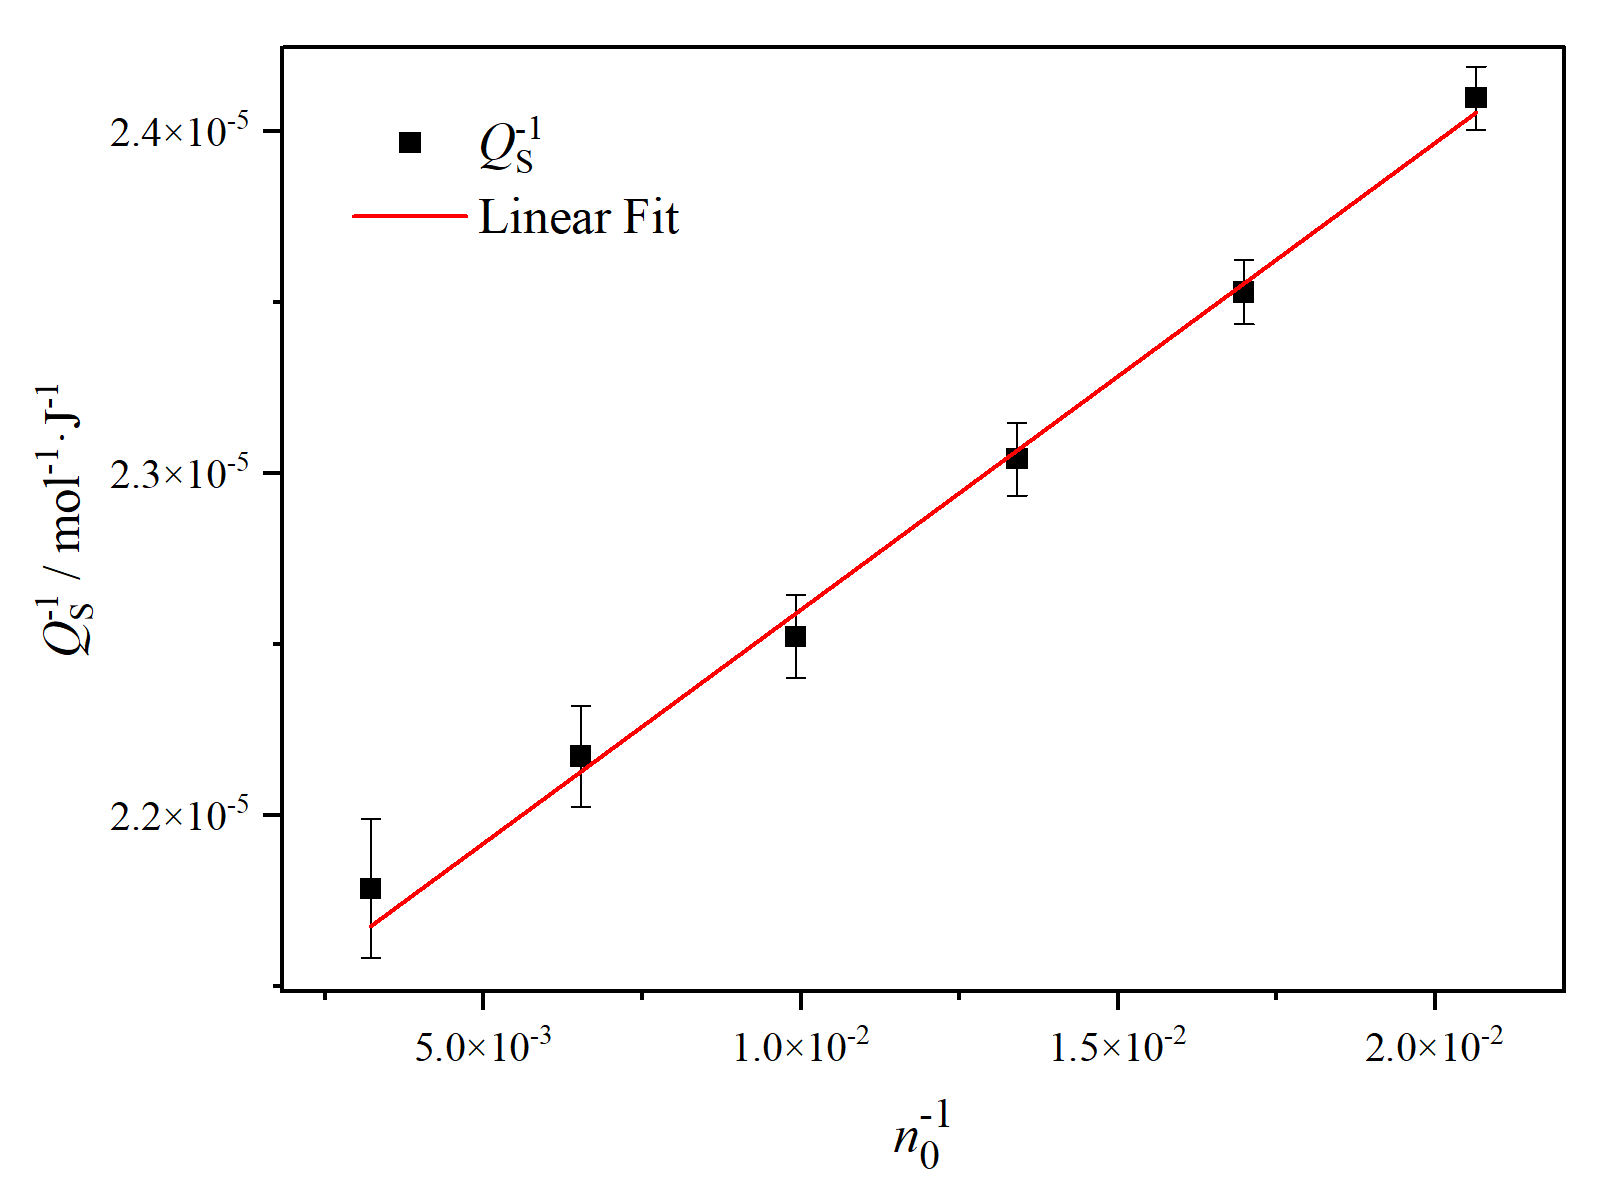
\includegraphics[width=.7\textwidth]{figures/5-2.png}
    \caption{$Q_{\mathrm{s}}^{-1}-n_0^{-1}$的拟合直线}
    \label{fig:7}
\end{figure}

拟合直线的表达式为
\begin{equation*}
    Q_{\mathrm{s}}^{-1}/\mathrm{J\cdot mol^{-1}} = (2.124 \pm 0.007 )\times 10^{-5} + (1.364 \pm 0.045 ) \times 10^{-4}n_0^{-1} \quad r^2 = 0.9956
\end{equation*}

最终,得到拟合公式 \eqref{eq:11} 中的参数:
\begin{align*}
    \frac{1}{Q_{\mathrm{s}}^0} &= (2.124 \pm 0.007 )\times 10^{-5}  \\
    \therefore Q_{\mathrm{s}}^0 &= 4.70 \times 10^4 \mathrm{~J\cdot mol^{-1}}\\
    a &= \frac{1}{1.364\times 10^{-4}\times 4.70 \times 10^4} = 0.156 \\
    \sigma_{Q_{\mathrm{s}}} &= \frac{0.007\times 10^{-5}}{(2.124\times 10^{-5})^2} = 1.6\times 10^2\\
    \therefore  Q_{\mathrm{s}}^0 &= (4.70 \pm 0.02)\times 10^4 \mathrm{~J\cdot mol^{-1}}
\end{align*}
对比式 \eqref{eq:7} 中,$Q_{\mathrm{s}}-n_0^{-1}$拟合得到的:
\begin{equation}
     Q_{\mathrm{s}}^0 = (4.69 \pm 0.01)\times 10^4 \mathrm{~J\cdot mol^{-1}}
\end{equation}
并没有显著区别,可以认为两种拟合方法都具有一定的合理性。
\subsubsection{溶解热平均偏差的求算}

在 \ref{sec:1} 的 \ref{tab:13} 中,已经计算得到了溶剂热偏差,如表 \ref{tab:17}。

\begin{table}[htbp]
    \centering
    \caption{补偿热、溶解热及其各自不确定度}
    \begin{tabular}{ccc}
        \toprule
        实验序号 & $\mathrm{d}Q/\mathrm{J}$ \\
        \midrule
        1 & 38 \\
        2 & 38 \\
        3 & 37 \\
        4 & 36 \\
        5 & 35 \\
        6 & 34 \\
        \bottomrule
    \end{tabular}
    \label{tab:17}
\end{table}

其平均偏差为:
\begin{equation*}
    \overline{\mathrm{d}Q} = 36\mathrm{~J}
\end{equation*}

\subsubsection{体系环境热交换的校正方法}

本实验中主要是用来了两种校正方法:
\begin{itemize}
    \item \textbf{雷诺校正}:使用雷诺校正法,校正体系的温差变化,减小体系与环境热交换的误差。
    \item \textbf{斜率校正}:通过升降温过程相邻的平台期温度-时间拟合直线的平均值,来代表升降温过程的体系-环境热交换导致的温度变化率,以校正误差。
\end{itemize}
\subsection{总结}

查阅文献\cite{haynes2016crc},得到\ce{KNO_3}的标准溶解焓,即微分溶解热:
\begin{equation*}
    \Delta H_{\mathrm{s}}(\ce{KNO_3}) = Q_{\mathrm{s}} = 34.89 \mathrm{~kJ\cdot mol^{-1}}
\end{equation*}

所以,本次实验的偏差为:
\begin{equation*}
    E_r(Q_\mathrm{S}) = \frac{47.0-34.9}{34.9}\times 100\% = + 35\%
\end{equation*}
由此可见,本实验中具有较大的正误差,这可能是由于,电阻丝的发热并没有100\%被溶液吸收。也就是说在实验中,电阻丝可能有一部分没有浸没入溶液,导致其与空气接触发生热传导,使得其一部分发热被散失到空气中。
\subsection{意见与建议}
\begin{itemize}
    \item 本实验中,两轮实验可以分别测定不同的溶质溶解的热效应,以比较两者的不同溶质溶解的区别,本次实验中两轮实验的数据重复,可供分析的数据并不多。
    \item 可以使用更为精密的溶解热测定装置,而不是简单的使用保温杯改造。保温杯气密性很差,导致体系中的空气会与外界发生交换,进而使得热交换加快,体系不绝热。
    \item 可以使用搅拌仪而不是磁子进行搅拌,磁子会与保温杯底部发生明显的摩擦生热,根据我的观察,大部分保温杯底部已有非常明显的磨损、生锈,这会一定程度上造成实验误差:因为磁子的转速无法真正准确控制,当溶液在不断溶解溶质的过程中,其粘度也在逐渐增加,导致虽然磁力搅拌仪转速设置相同,前后磁子的转速也无法保证完全一致。
\end{itemize}


\bibliography{wreference}

\section*{\quad 附录:原始数据}

{\tiny

\begin{longtable}{cc|cc|cc|cc|cc|cc|cc|cc|cc|cc}
\toprule
\endhead

\caption{Loop1-1温度-时间关系}\\
\toprule
$t$/\si{s} & $\Delta T$/\si{K} & $t$/\si{s} & $\Delta T$/\si{K} & $t$/\si{s} & $\Delta T$/\si{K} & $t$/\si{s} & $\Delta T$/\si{K} & $t$/\si{s} & $\Delta T$/\si{K} & $t$/\si{s} & $\Delta T$/\si{K} & $t$/\si{s} & $\Delta T$/\si{K} & $t$/\si{s} & $\Delta T$/\si{K} & $t$/\si{s} & $\Delta T$/\si{K} & $t$/\si{s} & $\Delta T$/\si{K} \\
\midrule
\endfirsthead

\bottomrule
\endfoot

\bottomrule
\endlastfoot

1.102 & 0.001 & 134.376 & -1.74 & 265.53 & -2.811 & 395.575 & -2.45 & 525.858 & -1.876 & 656.355 & -1.29 & 788.589 & -0.698 & 921.413 & -0.103 & 1054.092 & 0.143 & 1186.917 & 0.175 \\
1.734 & 0.001 & 135.066 & -1.775 & 266.222 & -2.81 & 396.208 & -2.448 & 526.63 & -1.872 & 657.069 & -1.288 & 789.362 & -0.694 & 922.046 & -0.101 & 1054.864 & 0.143 & 1187.548 & 0.174 \\
2.507 & 0.002 & 135.781 & -1.793 & 266.936 & -2.811 & 396.898 & -2.443 & 527.263 & -1.87 & 657.759 & -1.284 & 789.994 & -0.692 & 922.819 & -0.097 & 1055.497 & 0.143 & 1188.321 & 0.174 \\
3.14 & 0.001 & 136.471 & -1.828 & 267.627 & -2.81 & 397.613 & -2.441 & 528.035 & -1.866 & 658.473 & -1.282 & 790.767 & -0.688 & 923.45 & -0.095 & 1056.269 & 0.144 & 1189.034 & 0.174 \\
3.913 & 0.002 & 137.104 & -1.845 & 268.259 & -2.809 & 398.304 & -2.436 & 528.668 & -1.864 & 659.165 & -1.278 & 791.398 & -0.686 & 924.223 & -0.091 & 1056.983 & 0.144 & 1189.725 & 0.175 \\
4.545 & 0.001 & 137.877 & -1.881 & 269.031 & -2.811 & 398.936 & -2.435 & 529.441 & -1.859 & 659.797 & -1.275 & 792.171 & -0.681 & 924.855 & -0.089 & 1057.673 & 0.145 & 1190.358 & 0.175 \\
5.319 & 0.001 & 138.591 & -1.898 & 269.664 & -2.81 & 399.569 & -2.433 & 530.072 & -1.857 & 660.569 & -1.271 & 792.804 & -0.679 & 925.628 & -0.085 & 1058.306 & 0.145 & 1191.129 & 0.175 \\
5.951 & 0.001 & 139.282 & -1.931 & 270.437 & -2.809 & 400.258 & -2.429 & 530.845 & -1.852 & 661.202 & -1.269 & 793.576 & -0.675 & 926.342 & -0.082 & 1059.078 & 0.145 & 1191.761 & 0.176 \\
6.724 & 0.001 & 139.996 & -1.948 & 271.07 & -2.809 & 400.974 & -2.428 & 531.56 & -1.851 & 661.975 & -1.265 & 794.291 & -0.673 & 927.033 & -0.078 & 1059.792 & 0.145 & 1192.535 & 0.175 \\
7.356 & 0.001 & 140.687 & -1.979 & 271.842 & -2.809 & 401.664 & -2.423 & 532.251 & -1.847 & 662.607 & -1.262 & 794.981 & -0.669 & 927.664 & -0.076 & 1060.482 & 0.145 & 1193.166 & 0.175 \\
8.129 & 0.001 & 141.32 & -1.993 & 272.557 & -2.809 & 402.296 & -2.421 & 532.883 & -1.845 & 663.379 & -1.259 & 795.614 & -0.666 & 928.437 & -0.073 & 1061.116 & 0.146 & 1193.939 & 0.176 \\
8.761 & 0.001 & 142.092 & -2.024 & 273.247 & -2.809 & 402.988 & -2.418 & 533.655 & -1.84 & 664.094 & -1.256 & 796.385 & -0.662 & 929.07 & -0.07 & 1061.887 & 0.146 & 1194.571 & 0.176 \\
9.534 & 0.002 & 142.806 & -2.039 & 273.88 & -2.809 & 403.619 & -2.415 & 534.289 & -1.838 & 664.784 & -1.252 & 797.018 & -0.66 & 929.843 & -0.066 & 1062.52 & 0.147 & 1195.344 & 0.176 \\
10.167 & 0.002 & 143.498 & -2.069 & 274.512 & -2.809 & 404.392 & -2.411 & 534.921 & -1.836 & 665.417 & -1.25 & 797.791 & -0.656 & 930.474 & -0.064 & 1063.293 & 0.147 & 1195.976 & 0.176 \\
10.94 & 0.002 & 144.13 & -2.083 & 275.202 & -2.808 & 405.107 & -2.409 & 535.61 & -1.832 & 666.19 & -1.245 & 798.423 & -0.655 & 931.247 & -0.06 & 1063.924 & 0.147 & 1196.748 & 0.176 \\
11.573 & 0.001 & 144.763 & -2.097 & 275.835 & -2.809 & 405.797 & -2.405 & 536.244 & -1.829 & 666.906 & -1.243 & 799.195 & -0.649 & 931.878 & -0.057 & 1064.697 & 0.147 & 1197.462 & 0.177 \\
12.345 & 0.001 & 145.453 & -2.125 & 276.525 & -2.808 & 406.511 & -2.403 & 536.934 & -1.825 & 667.594 & -1.239 & 799.828 & -0.647 & 932.651 & -0.053 & 1065.412 & 0.148 & 1198.153 & 0.177 \\
12.977 & 0.002 & 146.156 & -2.139 & 277.24 & -2.809 & 407.203 & -2.399 & 537.648 & -1.824 & 668.309 & -1.237 & 800.6 & -0.643 & 933.284 & -0.051 & 1066.101 & 0.148 & 1198.867 & 0.177 \\
13.751 & 0.002 & 146.776 & -2.164 & 277.931 & -2.808 & 407.835 & -2.396 & 538.339 & -1.819 & 668.999 & -1.233 & 801.232 & -0.641 & 934.057 & -0.047 & 1066.734 & 0.148 & 1199.558 & 0.177 \\
14.383 & 0.002 & 147.409 & -2.177 & 278.564 & -2.808 & 408.607 & -2.393 & 538.971 & -1.817 & 669.631 & -1.23 & 802.005 & -0.638 & 934.688 & -0.045 & 1067.506 & 0.148 & 1200.189 & 0.177 \\
15.156 & 0.002 & 148.181 & -2.201 & 279.337 & -2.808 & 409.321 & -2.391 & 539.603 & -1.815 & 670.404 & -1.227 & 802.719 & -0.635 & 935.461 & -0.041 & 1068.138 & 0.148 & 1200.963 & 0.177 \\
15.871 & 0.002 & 148.814 & -2.214 & 279.969 & -2.808 & 410.012 & -2.387 & 540.294 & -1.811 & 671.036 & -1.225 & 803.41 & -0.631 & 936.094 & -0.038 & 1068.911 & 0.148 & 1201.594 & 0.176 \\
16.561 & 0.002 & 149.587 & -2.237 & 280.602 & -2.807 & 410.727 & -2.385 & 540.927 & -1.809 & 671.81 & -1.22 & 804.043 & -0.628 & 936.866 & -0.034 & 1069.543 & 0.149 & 1202.366 & 0.178 \\
17.194 & 0.001 & 150.302 & -2.25 & 281.292 & -2.807 & 411.418 & -2.381 & 541.617 & -1.804 & 672.523 & -1.219 & 804.815 & -0.624 & 937.58 & -0.033 & 1070.316 & 0.149 & 1203 & 0.177 \\
17.966 & 0.001 & 150.993 & -2.274 & 281.924 & -2.807 & 412.05 & -2.379 & 542.25 & -1.802 & 673.213 & -1.215 & 805.529 & -0.622 & 938.271 & -0.028 & 1070.949 & 0.149 & 1203.772 & 0.177 \\
18.682 & 0.002 & 151.625 & -2.285 & 282.616 & -2.807 & 412.683 & -2.376 & 542.881 & -1.801 & 673.846 & -1.212 & 806.22 & -0.618 & 938.985 & -0.026 & 1071.721 & 0.149 & 1204.404 & 0.177 \\
19.372 & 0.002 & 152.258 & -2.296 & 283.247 & -2.806 & 413.373 & -2.372 & 543.572 & -1.797 & 674.479 & -1.209 & 806.852 & -0.616 & 939.675 & -0.021 & 1072.353 & 0.149 & 1205.177 & 0.178 \\
20.004 & 0.002 & 152.949 & -2.321 & 284.02 & -2.806 & 414.088 & -2.371 & 544.206 & -1.794 & 675.169 & -1.206 & 807.625 & -0.611 & 940.308 & -0.02 & 1073.125 & 0.15 & 1205.891 & 0.178 \\
20.777 & 0.001 & 153.581 & -2.336 & 284.652 & -2.806 & 414.779 & -2.366 & 544.895 & -1.79 & 676.023 & -1.202 & 808.256 & -0.61 & 941.08 & -0.016 & 1073.757 & 0.15 & 1206.581 & 0.177 \\
21.491 & 0.002 & 154.272 & -2.366 & 285.426 & -2.807 & 415.411 & -2.364 & 545.528 & -1.788 & 676.656 & -1.2 & 809.029 & -0.605 & 941.712 & -0.014 & 1074.53 & 0.15 & 1207.295 & 0.178 \\
22.183 & 0.002 & 154.986 & -2.381 & 286.057 & -2.807 & 416.101 & -2.361 & 546.301 & -1.784 & 677.429 & -1.195 & 809.743 & -0.603 & 942.485 & -0.009 & 1075.244 & 0.15 & 1207.985 & 0.178 \\
22.816 & 0.002 & 155.677 & -2.415 & 286.69 & -2.806 & 416.734 & -2.359 & 547.015 & -1.782 & 678.061 & -1.193 & 810.434 & -0.599 & 943.2 & -0.008 & 1075.935 & 0.151 & 1208.618 & 0.178 \\
23.589 & 0.001 & 156.309 & -2.432 & 287.381 & -2.806 & 417.506 & -2.354 & 547.706 & -1.777 & 678.834 & -1.189 & 811.148 & -0.597 & 943.89 & -0.003 & 1076.649 & 0.151 & 1209.39 & 0.179 \\
24.221 & 0.002 & 157.082 & -2.465 & 288.014 & -2.805 & 418.139 & -2.352 & 548.339 & -1.775 & 679.466 & -1.186 & 811.839 & -0.593 & 944.522 & -0.002 & 1077.34 & 0.151 & 1210.022 & 0.179 \\
24.994 & 0.002 & 157.714 & -2.483 & 288.704 & -2.805 & 418.911 & -2.349 & 549.111 & -1.771 & 680.238 & -1.183 & 812.553 & -0.591 & 945.294 & 0.002 & 1077.972 & 0.151 & 1210.796 & 0.178 \\
25.708 & 0.002 & 158.487 & -2.516 & 289.419 & -2.804 & 419.544 & -2.346 & 549.742 & -1.769 & 680.87 & -1.181 & 813.244 & -0.587 & 946.008 & 0.004 & 1078.744 & 0.151 & 1211.427 & 0.178 \\
26.399 & 0.001 & 159.12 & -2.532 & 290.109 & -2.804 & 420.316 & -2.342 & 550.516 & -1.765 & 681.643 & -1.177 & 813.958 & -0.585 & 946.699 & 0.007 & 1079.376 & 0.151 & 1212.199 & 0.178 \\
27.031 & 0.002 & 159.893 & -2.563 & 290.744 & -2.803 & 420.949 & -2.34 & 551.148 & -1.763 & 682.276 & -1.174 & 814.649 & -0.581 & 947.413 & 0.009 & 1080.149 & 0.152 & 1212.913 & 0.179 \\
27.805 & 0.002 & 160.525 & -2.577 & 291.514 & -2.803 & 421.581 & -2.338 & 551.78 & -1.761 & 682.909 & -1.172 & 815.281 & -0.579 & 948.104 & 0.012 & 1080.78 & 0.152 & 1213.604 & 0.178 \\
28.437 & 0.002 & 161.298 & -2.604 & 292.146 & -2.802 & 422.272 & -2.334 & 552.471 & -1.755 & 683.598 & -1.168 & 816.054 & -0.574 & 948.736 & 0.014 & 1081.553 & 0.152 & 1214.237 & 0.18 \\
29.21 & 0.002 & 162.012 & -2.617 & 292.92 & -2.802 & 422.904 & -2.333 & 553.103 & -1.753 & 684.231 & -1.166 & 816.686 & -0.572 & 949.508 & 0.018 & 1082.268 & 0.152 & 1215.009 & 0.179 \\
29.843 & 0.001 & 162.703 & -2.64 & 293.552 & -2.802 & 423.594 & -2.328 & 553.794 & -1.75 & 684.921 & -1.162 & 817.459 & -0.568 & 950.141 & 0.019 & 1082.958 & 0.153 & 1215.641 & 0.179 \\
30.615 & 0.003 & 163.336 & -2.651 & 294.325 & -2.801 & 424.309 & -2.325 & 554.426 & -1.748 & 685.636 & -1.159 & 818.091 & -0.566 & 950.914 & 0.022 & 1083.594 & 0.153 & 1216.413 & 0.18 \\
31.247 & 0.003 & 164.108 & -2.671 & 295.039 & -2.801 & 424.999 & -2.321 & 555.198 & -1.744 & 686.326 & -1.156 & 818.864 & -0.562 & 951.545 & 0.024 & 1084.363 & 0.154 & 1217.046 & 0.179 \\
32.02 & 0.003 & 164.741 & -2.682 & 295.73 & -2.799 & 425.633 & -2.319 & 555.831 & -1.742 & 686.959 & -1.153 & 819.495 & -0.56 & 952.318 & 0.027 & 1084.995 & 0.153 & 1217.818 & 0.179 \\
32.653 & 0.003 & 165.514 & -2.699 & 296.363 & -2.798 & 426.405 & -2.315 & 556.604 & -1.738 & 687.591 & -1.151 & 820.267 & -0.555 & 952.951 & 0.028 & 1085.768 & 0.154 & 1218.45 & 0.18 \\
33.425 & 0.002 & 166.145 & -2.707 & 297.135 & -2.797 & 427.119 & -2.313 & 557.318 & -1.736 & 688.2 & -1.148 & 820.982 & -0.553 & 953.723 & 0.032 & 1086.4 & 0.153 & 1219.223 & 0.18 \\
34.141 & 0.002 & 166.778 & -2.715 & 297.767 & -2.796 & 427.81 & -2.309 & 558.008 & -1.732 & 688.913 & -1.145 & 821.673 & -0.549 & 954.356 & 0.033 & 1087.172 & 0.154 & 1219.855 & 0.18 \\
34.832 & 0.002 & 167.458 & -2.728 & 298.54 & -2.796 & 428.524 & -2.307 & 558.723 & -1.729 & 689.604 & -1.141 & 822.305 & -0.547 & 955.128 & 0.036 & 1087.804 & 0.154 & 1220.627 & 0.18 \\
35.464 & 0.002 & 168.102 & -2.734 & 299.173 & -2.795 & 429.215 & -2.304 & 559.414 & -1.725 & 690.318 & -1.139 & 823.078 & -0.543 & 955.76 & 0.037 & 1088.577 & 0.154 & 1221.259 & 0.18 \\
36.237 & 0.003 & 168.792 & -2.746 & 299.945 & -2.794 & 429.929 & -2.302 & 560.045 & -1.723 & 691.01 & -1.134 & 823.709 & -0.541 & 956.533 & 0.04 & 1089.291 & 0.155 & 1222.032 & 0.18 \\
36.87 & 0.003 & 169.507 & -2.752 & 300.578 & -2.793 & 430.62 & -2.297 & 560.819 & -1.718 & 691.641 & -1.133 & 824.482 & -0.537 & 957.165 & 0.041 & 1089.981 & 0.154 & 1222.664 & 0.179 \\
37.643 & 0.002 & 170.197 & -2.761 & 301.21 & -2.792 & 431.252 & -2.296 & 561.451 & -1.716 & 692.414 & -1.128 & 825.197 & -0.535 & 957.937 & 0.044 & 1090.614 & 0.155 & 1223.437 & 0.18 \\
38.357 & 0.003 & 170.83 & -2.765 & 301.9 & -2.79 & 432.025 & -2.291 & 562.223 & -1.712 & 693.046 & -1.125 & 825.887 & -0.531 & 958.57 & 0.045 & 1091.386 & 0.155 & 1224.068 & 0.18 \\
39.047 & 0.003 & 171.603 & -2.772 & 302.533 & -2.789 & 432.74 & -2.289 & 562.856 & -1.71 & 693.82 & -1.121 & 826.602 & -0.528 & 959.343 & 0.047 & 1092.019 & 0.155 & 1224.841 & 0.181 \\
39.68 & 0.002 & 172.235 & -2.776 & 303.224 & -2.788 & 433.43 & -2.284 & 563.628 & -1.706 & 694.451 & -1.12 & 827.292 & -0.524 & 960.056 & 0.049 & 1092.791 & 0.155 & 1225.473 & 0.18 \\
40.452 & 0.002 & 173.008 & -2.782 & 303.938 & -2.788 & 434.063 & -2.283 & 564.261 & -1.704 & 695.224 & -1.116 & 828.006 & -0.522 & 960.747 & 0.051 & 1093.422 & 0.156 & 1226.246 & 0.181 \\
41.085 & 0.002 & 173.723 & -2.785 & 304.63 & -2.786 & 434.836 & -2.279 & 565.034 & -1.7 & 695.938 & -1.114 & 828.697 & -0.518 & 961.461 & 0.053 & 1094.196 & 0.156 & 1226.877 & 0.18 \\
41.859 & 0.002 & 174.413 & -2.791 & 305.262 & -2.784 & 435.467 & -2.277 & 565.748 & -1.698 & 696.629 & -1.109 & 829.41 & -0.515 & 962.151 & 0.055 & 1094.828 & 0.156 & 1227.651 & 0.181 \\
42.491 & 0.002 & 175.046 & -2.793 & 306.034 & -2.782 & 436.24 & -2.273 & 566.438 & -1.694 & 697.343 & -1.108 & 830.102 & -0.512 & 962.784 & 0.057 & 1095.6 & 0.156 & 1228.365 & 0.181 \\
43.263 & 0.003 & 175.82 & -2.797 & 306.667 & -2.781 & 436.873 & -2.271 & 567.071 & -1.691 & 698.034 & -1.104 & 830.734 & -0.51 & 963.557 & 0.059 & 1096.232 & 0.156 & 1229.055 & 0.181 \\
43.897 & 0.003 & 176.534 & -2.8 & 307.439 & -2.779 & 437.645 & -2.267 & 567.703 & -1.689 & 698.669 & -1.102 & 831.506 & -0.505 & 964.188 & 0.06 & 1097.005 & 0.157 & 1229.688 & 0.181 \\
44.669 & 0.003 & 177.224 & -2.803 & 308.071 & -2.778 & 438.278 & -2.265 & 568.394 & -1.685 & 699.438 & -1.097 & 832.14 & -0.502 & 964.961 & 0.062 & 1097.719 & 0.156 & 1230.46 & 0.181 \\
45.383 & 0.003 & 177.856 & -2.805 & 308.845 & -2.776 & 438.91 & -2.262 & 569.026 & -1.682 & 700.152 & -1.094 & 832.911 & -0.5 & 965.675 & 0.063 & 1098.41 & 0.156 & 1231.092 & 0.181 \\
46.074 & 0.002 & 178.489 & -2.806 & 309.477 & -2.775 & 439.601 & -2.258 & 569.717 & -1.679 & 700.844 & -1.091 & 833.544 & -0.497 & 966.365 & 0.065 & 1099.042 & 0.157 & 1231.865 & 0.181 \\
46.788 & 0.002 & 179.18 & -2.81 & 310.11 & -2.774 & 440.315 & -2.256 & 570.431 & -1.677 & 701.475 & -1.089 & 834.317 & -0.493 & 966.998 & 0.066 & 1099.814 & 0.157 & 1232.496 & 0.182 \\
47.48 & 0.002 & 179.812 & -2.81 & 310.799 & -2.771 & 441.007 & -2.252 & 571.123 & -1.672 & 702.248 & -1.084 & 834.949 & -0.491 & 967.771 & 0.068 & 1100.528 & 0.157 & 1233.269 & 0.182 \\
48.112 & 0.002 & 180.503 & -2.813 & 311.432 & -2.77 & 441.638 & -2.25 & 571.754 & -1.671 & 702.881 & -1.082 & 835.721 & -0.486 & 968.403 & 0.069 & 1101.219 & 0.158 & 1233.984 & 0.182 \\
48.885 & 0.003 & 181.218 & -2.814 & 312.124 & -2.768 & 442.329 & -2.246 & 572.526 & -1.666 & 703.653 & -1.078 & 836.435 & -0.484 & 969.176 & 0.071 & 1101.851 & 0.158 & 1234.674 & 0.182 \\
49.518 & 0.003 & 181.908 & -2.815 & 312.755 & -2.767 & 443.043 & -2.244 & 573.16 & -1.664 & 704.298 & -1.076 & 837.126 & -0.48 & 969.807 & 0.072 & 1102.624 & 0.158 & 1235.388 & 0.182 \\
50.29 & 0.003 & 182.54 & -2.817 & 313.528 & -2.764 & 443.734 & -2.239 & 573.791 & -1.663 & 705.07 & -1.072 & 837.759 & -0.478 & 970.58 & 0.074 & 1103.255 & 0.158 & 1236.078 & 0.182 \\
50.923 & 0.003 & 183.313 & -2.818 & 314.16 & -2.763 & 444.367 & -2.239 & 574.483 & -1.658 & 705.785 & -1.07 & 838.531 & -0.473 & 971.212 & 0.074 & 1104.029 & 0.158 & 1236.71 & 0.182 \\
51.696 & 0.003 & 184.028 & -2.819 & 314.934 & -2.76 & 445.139 & -2.234 & 575.114 & -1.656 & 706.474 & -1.065 & 839.245 & -0.472 & 971.985 & 0.076 & 1104.743 & 0.158 & 1237.482 & 0.182 \\
52.41 & 0.003 & 184.719 & -2.82 & 315.566 & -2.76 & 445.853 & -2.232 & 575.806 & -1.651 & 707.107 & -1.063 & 839.935 & -0.467 & 972.7 & 0.077 & 1105.433 & 0.159 & 1238.116 & 0.182 \\
53.101 & 0.003 & 185.352 & -2.82 & 316.199 & -2.758 & 446.544 & -2.227 & 576.437 & -1.65 & 707.879 & -1.059 & 840.567 & -0.466 & 973.389 & 0.079 & 1106.066 & 0.158 & 1238.887 & 0.183 \\
53.734 & 0.003 & 185.984 & -2.821 & 316.888 & -2.755 & 447.176 & -2.226 & 577.21 & -1.645 & 708.512 & -1.057 & 841.34 & -0.461 & 974.104 & 0.08 & 1106.837 & 0.159 & 1239.52 & 0.183 \\
54.506 & 0.002 & 186.674 & -2.822 & 317.521 & -2.753 & 447.949 & -2.222 & 577.843 & -1.644 & 709.284 & -1.053 & 842.054 & -0.459 & 974.795 & 0.081 & 1107.47 & 0.159 & 1240.292 & 0.182 \\
55.139 & 0.003 & 187.307 & -2.822 & 318.212 & -2.751 & 448.582 & -2.219 & 578.615 & -1.639 & 709.916 & -1.051 & 842.746 & -0.455 & 975.509 & 0.082 & 1108.246 & 0.159 & 1241.006 & 0.183 \\
55.912 & 0.003 & 187.998 & -2.823 & 318.845 & -2.749 & 449.354 & -2.215 & 579.247 & -1.637 & 710.689 & -1.046 & 843.377 & -0.453 & 976.199 & 0.083 & 1108.875 & 0.159 & 1241.697 & 0.182 \\
56.626 & 0.003 & 188.712 & -2.823 & 319.476 & -2.748 & 449.987 & -2.213 & 580.02 & -1.632 & 711.322 & -1.044 & 844.15 & -0.449 & 976.831 & 0.084 & 1109.647 & 0.16 & 1242.329 & 0.183 \\
57.317 & 0.003 & 189.403 & -2.823 & 320.085 & -2.746 & 450.62 & -2.211 & 580.652 & -1.63 & 712.094 & -1.04 & 844.864 & -0.446 & 977.604 & 0.086 & 1110.279 & 0.159 & 1243.102 & 0.183 \\
57.95 & 0.003 & 190.105 & -2.824 & 320.718 & -2.744 & 451.31 & -2.207 & 581.285 & -1.629 & 712.726 & -1.038 & 845.555 & -0.442 & 978.318 & 0.086 & 1111.052 & 0.16 & 1243.734 & 0.183 \\
58.723 & 0.003 & 190.808 & -2.824 & 321.49 & -2.741 & 451.942 & -2.204 & 581.975 & -1.624 & 713.499 & -1.034 & 846.187 & -0.44 & 979.009 & 0.088 & 1111.684 & 0.16 & 1244.506 & 0.184 \\
59.354 & 0.003 & 191.441 & -2.825 & 322.124 & -2.74 & 452.633 & -2.201 & 582.608 & -1.622 & 714.131 & -1.031 & 846.96 & -0.436 & 979.641 & 0.089 & 1112.456 & 0.16 & 1245.139 & 0.183 \\
60.127 & 0.003 & 192.213 & -2.824 & 322.896 & -2.737 & 453.347 & -2.198 & 583.298 & -1.619 & 714.904 & -1.027 & 847.674 & -0.434 & 980.413 & 0.09 & 1113.17 & 0.16 & 1245.91 & 0.183 \\
60.76 & 0.002 & 192.845 & -2.825 & 323.528 & -2.735 & 454.038 & -2.194 & 583.931 & -1.616 & 715.536 & -1.024 & 848.364 & -0.43 & 981.045 & 0.09 & 1113.862 & 0.16 & 1246.624 & 0.184 \\
61.533 & 0.003 & 193.619 & -2.825 & 324.16 & -2.734 & 454.751 & -2.192 & 584.562 & -1.614 & 716.309 & -1.021 & 848.996 & -0.428 & 981.818 & 0.092 & 1114.576 & 0.16 & 1247.316 & 0.184 \\
62.165 & 0.003 & 194.334 & -2.825 & 324.769 & -2.731 & 455.443 & -2.188 & 585.254 & -1.609 & 716.942 & -1.019 & 849.77 & -0.423 & 982.532 & 0.093 & 1115.266 & 0.16 & 1247.947 & 0.183 \\
62.938 & 0.003 & 195.024 & -2.825 & 325.403 & -2.729 & 456.076 & -2.186 & 585.886 & -1.608 & 717.714 & -1.015 & 850.401 & -0.421 & 983.223 & 0.094 & 1115.897 & 0.161 & 1248.72 & 0.184 \\
63.654 & 0.003 & 195.657 & -2.825 & 326.034 & -2.728 & 456.849 & -2.181 & 586.576 & -1.604 & 718.346 & -1.012 & 851.174 & -0.417 & 983.855 & 0.094 & 1116.67 & 0.161 & 1249.351 & 0.184 \\
64.344 & 0.003 & 196.429 & -2.826 & 326.725 & -2.724 & 457.563 & -2.18 & 587.209 & -1.601 & 719.119 & -1.008 & 851.806 & -0.415 & 984.628 & 0.096 & 1117.304 & 0.161 & 1250.124 & 0.184 \\
64.977 & 0.003 & 197.143 & -2.826 & 327.579 & -2.721 & 458.252 & -2.176 & 587.982 & -1.598 & 719.832 & -1.007 & 852.579 & -0.411 & 985.341 & 0.096 & 1118.075 & 0.161 & 1250.839 & 0.184 \\
65.749 & 0.004 & 197.834 & -2.826 & 328.212 & -2.72 & 458.967 & -2.174 & 588.613 & -1.595 & 720.523 & -1.002 & 853.211 & -0.409 & 986.032 & 0.098 & 1118.708 & 0.162 & 1251.529 & 0.184 \\
66.382 & 0.003 & 198.467 & -2.826 & 328.985 & -2.716 & 459.658 & -2.169 & 589.387 & -1.59 & 721.156 & -1 & 853.984 & -0.405 & 986.746 & 0.098 & 1119.48 & 0.162 & 1252.162 & 0.184 \\
67.155 & 0.003 & 199.24 & -2.826 & 329.699 & -2.715 & 460.29 & -2.168 & 590.018 & -1.588 & 721.929 & -0.996 & 854.616 & -0.403 & 987.437 & 0.1 & 1120.112 & 0.162 & 1252.934 & 0.184 \\
67.787 & 0.004 & 199.872 & -2.825 & 330.391 & -2.712 & 460.922 & -2.166 & 590.791 & -1.584 & 722.561 & -0.994 & 855.389 & -0.398 & 988.152 & 0.1 & 1120.885 & 0.162 & 1253.566 & 0.184 \\
68.56 & 0.004 & 200.644 & -2.826 & 331.023 & -2.71 & 461.613 & -2.161 & 591.424 & -1.582 & 723.333 & -0.99 & 856.103 & -0.396 & 988.842 & 0.101 & 1121.529 & 0.163 & 1254.338 & 0.184 \\
69.192 & 0.003 & 201.277 & -2.826 & 331.795 & -2.707 & 462.246 & -2.16 & 592.056 & -1.581 & 724.048 & -0.987 & 856.793 & -0.392 & 989.556 & 0.102 & 1122.29 & 0.162 & 1255.053 & 0.185 \\
69.965 & 0.004 & 202.05 & -2.825 & 332.429 & -2.705 & 462.936 & -2.155 & 592.747 & -1.576 & 724.738 & -0.984 & 857.507 & -0.389 & 990.246 & 0.103 & 1122.921 & 0.162 & 1255.743 & 0.184 \\
70.598 & 0.004 & 202.764 & -2.825 & 333.2 & -2.702 & 463.569 & -2.152 & 593.601 & -1.572 & 725.371 & -0.981 & 858.198 & -0.386 & 990.96 & 0.104 & 1123.706 & 0.163 & 1256.457 & 0.184 \\
71.37 & 0.003 & 203.456 & -2.825 & 333.832 & -2.7 & 464.201 & -2.151 & 594.234 & -1.57 & 726.142 & -0.977 & 858.83 & -0.384 & 991.651 & 0.104 & 1124.42 & 0.164 & 1257.148 & 0.185 \\
72.003 & 0.003 & 204.171 & -2.825 & 334.606 & -2.696 & 464.81 & -2.147 & 594.866 & -1.568 & 726.857 & -0.975 & 859.603 & -0.379 & 992.283 & 0.105 & 1125.099 & 0.162 & 1257.862 & 0.185 \\
72.776 & 0.004 & 204.861 & -2.825 & 335.238 & -2.694 & 465.442 & -2.144 & 595.557 & -1.564 & 727.548 & -0.971 & 860.235 & -0.377 & 993.056 & 0.106 & 1125.742 & 0.163 & 1258.552 & 0.185 \\
73.408 & 0.004 & 205.494 & -2.825 & 336.01 & -2.692 & 466.215 & -2.14 & 596.188 & -1.561 & 728.18 & -0.969 & 861.007 & -0.374 & 993.689 & 0.107 & 1126.515 & 0.163 & 1259.184 & 0.184 \\
74.181 & 0.004 & 206.266 & -2.825 & 336.644 & -2.69 & 466.847 & -2.139 & 596.879 & -1.558 & 728.953 & -0.964 & 861.64 & -0.371 & 994.461 & 0.107 & 1127.23 & 0.163 & 1259.957 & 0.186 \\
74.896 & 0.004 & 206.899 & -2.825 & 337.275 & -2.688 & 467.62 & -2.134 & 597.593 & -1.555 & 729.667 & -0.963 & 862.413 & -0.367 & 995.093 & 0.108 & 1127.919 & 0.164 & 1260.671 & 0.185 \\
75.586 & 0.003 & 207.671 & -2.824 & 337.966 & -2.685 & 468.334 & -2.131 & 598.285 & -1.551 & 730.358 & -0.958 & 863.126 & -0.364 & 995.866 & 0.108 & 1128.552 & 0.164 & 1261.362 & 0.186 \\
76.301 & 0.004 & 208.385 & -2.824 & 338.681 & -2.683 & 469.025 & -2.128 & 598.998 & -1.549 & 731.072 & -0.957 & 863.817 & -0.361 & 996.497 & 0.108 & 1129.325 & 0.164 & 1261.994 & 0.186 \\
76.992 & 0.004 & 209.077 & -2.824 & 339.371 & -2.679 & 469.657 & -2.126 & 599.689 & -1.544 & 731.763 & -0.952 & 864.531 & -0.359 & 997.271 & 0.11 & 1129.956 & 0.164 & 1262.766 & 0.186 \\
77.706 & 0.004 & 209.791 & -2.823 & 340.004 & -2.677 & 470.43 & -2.122 & 600.404 & -1.541 & 732.395 & -0.951 & 865.223 & -0.355 & 997.903 & 0.11 & 1130.729 & 0.164 & 1263.399 & 0.186 \\
78.48 & 0.004 & 210.481 & -2.824 & 340.694 & -2.674 & 471.062 & -2.119 & 601.095 & -1.539 & 733.167 & -0.945 & 865.854 & -0.352 & 998.675 & 0.111 & 1131.361 & 0.164 & 1264.171 & 0.186 \\
79.112 & 0.004 & 211.113 & -2.824 & 341.327 & -2.672 & 471.695 & -2.118 & 601.726 & -1.537 & 733.799 & -0.943 & 866.626 & -0.348 & 999.308 & 0.112 & 1132.134 & 0.164 & 1264.803 & 0.186 \\
79.803 & 0.004 & 211.887 & -2.823 & 342.099 & -2.668 & 472.385 & -2.113 & 602.499 & -1.532 & 734.572 & -0.939 & 867.259 & -0.346 & 1000.081 & 0.112 & 1132.848 & 0.164 & 1265.576 & 0.186 \\
80.517 & 0.004 & 212.519 & -2.823 & 342.732 & -2.666 & 473.018 & -2.111 & 603.132 & -1.53 & 735.205 & -0.937 & 868.031 & -0.342 & 1000.712 & 0.113 & 1133.538 & 0.165 & 1266.207 & 0.186 \\
81.208 & 0.004 & 213.292 & -2.823 & 343.364 & -2.665 & 473.709 & -2.107 & 603.904 & -1.526 & 735.977 & -0.933 & 868.745 & -0.34 & 1001.485 & 0.114 & 1134.171 & 0.165 & 1266.98 & 0.186 \\
81.923 & 0.005 & 214.007 & -2.823 & 344.055 & -2.661 & 474.34 & -2.105 & 604.537 & -1.524 & 736.609 & -0.93 & 869.437 & -0.336 & 1002.117 & 0.114 & 1134.943 & 0.165 & 1267.694 & 0.186 \\
82.613 & 0.004 & 214.698 & -2.822 & 344.687 & -2.659 & 475.113 & -2.101 & 605.309 & -1.519 & 737.382 & -0.926 & 870.069 & -0.333 & 1002.889 & 0.115 & 1135.657 & 0.165 & 1268.385 & 0.186 \\
83.245 & 0.004 & 215.33 & -2.823 & 345.379 & -2.655 & 475.746 & -2.098 & 605.941 & -1.517 & 738.096 & -0.925 & 870.841 & -0.329 & 1003.603 & 0.115 & 1136.348 & 0.165 & 1269.016 & 0.186 \\
84.018 & 0.004 & 216.103 & -2.822 & 346.092 & -2.654 & 476.378 & -2.097 & 606.714 & -1.513 & 738.787 & -0.92 & 871.474 & -0.327 & 1004.295 & 0.116 & 1136.98 & 0.166 & 1269.79 & 0.187 \\
84.651 & 0.004 & 216.816 & -2.821 & 346.784 & -2.65 & 477.068 & -2.093 & 607.428 & -1.51 & 739.419 & -0.919 & 872.246 & -0.323 & 1005.008 & 0.116 & 1137.753 & 0.166 & 1270.503 & 0.186 \\
85.423 & 0.004 & 217.508 & -2.822 & 347.498 & -2.648 & 477.923 & -2.089 & 608.119 & -1.507 & 740.192 & -0.915 & 872.878 & -0.321 & 1005.699 & 0.117 & 1138.385 & 0.166 & 1271.194 & 0.187 \\
86.056 & 0.004 & 218.141 & -2.821 & 348.188 & -2.645 & 478.556 & -2.086 & 608.751 & -1.504 & 740.906 & -0.912 & 873.651 & -0.317 & 1006.331 & 0.118 & 1139.157 & 0.166 & 1271.908 & 0.187 \\
86.829 & 0.004 & 218.773 & -2.821 & 348.821 & -2.643 & 479.329 & -2.083 & 609.524 & -1.5 & 741.597 & -0.908 & 874.283 & -0.314 & 1007.103 & 0.118 & 1139.789 & 0.167 & 1272.598 & 0.187 \\
87.543 & 0.004 & 219.464 & -2.822 & 349.593 & -2.639 & 479.962 & -2.08 & 610.156 & -1.498 & 742.311 & -0.906 & 875.055 & -0.311 & 1007.736 & 0.119 & 1140.562 & 0.166 & 1273.231 & 0.187 \\
88.234 & 0.004 & 220.096 & -2.822 & 350.226 & -2.637 & 480.733 & -2.076 & 610.929 & -1.494 & 743.002 & -0.901 & 875.689 & -0.309 & 1008.509 & 0.12 & 1141.194 & 0.167 & 1274.003 & 0.187 \\
88.95 & 0.004 & 220.786 & -2.822 & 350.999 & -2.634 & 481.366 & -2.074 & 611.561 & -1.492 & 743.633 & -0.899 & 876.46 & -0.305 & 1009.14 & 0.12 & 1141.967 & 0.167 & 1274.635 & 0.187 \\
89.64 & 0.004 & 221.42 & -2.822 & 351.631 & -2.632 & 481.998 & -2.072 & 612.333 & -1.487 & 744.407 & -0.895 & 877.174 & -0.302 & 1009.913 & 0.121 & 1142.598 & 0.167 & 1275.408 & 0.187 \\
90.272 & 0.005 & 222.192 & -2.821 & 352.263 & -2.631 & 482.689 & -2.068 & 612.967 & -1.485 & 745.039 & -0.893 & 877.866 & -0.298 & 1010.545 & 0.121 & 1143.372 & 0.167 & 1276.04 & 0.187 \\
91.045 & 0.004 & 222.824 & -2.821 & 352.954 & -2.627 & 483.321 & -2.066 & 613.739 & -1.481 & 745.811 & -0.888 & 878.497 & -0.296 & 1011.318 & 0.122 & 1144.004 & 0.167 & 1276.812 & 0.188 \\
91.678 & 0.005 & 223.596 & -2.82 & 353.587 & -2.625 & 484.012 & -2.061 & 614.454 & -1.479 & 746.526 & -0.887 & 879.27 & -0.291 & 1011.95 & 0.122 & 1144.776 & 0.167 & 1277.444 & 0.188 \\
92.45 & 0.004 & 224.229 & -2.82 & 354.277 & -2.62 & 484.644 & -2.06 & 615.144 & -1.475 & 747.216 & -0.882 & 879.902 & -0.29 & 1012.723 & 0.123 & 1145.408 & 0.167 & 1278.217 & 0.188 \\
93.083 & 0.004 & 225.002 & -2.82 & 354.991 & -2.619 & 485.417 & -2.056 & 615.858 & -1.473 & 747.93 & -0.881 & 880.674 & -0.285 & 1013.355 & 0.123 & 1146.18 & 0.168 & 1278.931 & 0.188 \\
93.855 & 0.004 & 225.635 & -2.82 & 355.681 & -2.615 & 486.049 & -2.054 & 616.549 & -1.468 & 748.621 & -0.876 & 881.307 & -0.283 & 1014.127 & 0.123 & 1146.812 & 0.167 & 1279.622 & 0.188 \\
94.488 & 0.004 & 226.267 & -2.82 & 356.315 & -2.614 & 486.822 & -2.05 & 617.18 & -1.466 & 749.253 & -0.874 & 882.079 & -0.279 & 1014.76 & 0.124 & 1147.585 & 0.167 & 1280.254 & 0.188 \\
95.261 & 0.004 & 226.957 & -2.82 & 357.087 & -2.609 & 487.454 & -2.047 & 617.953 & -1.463 & 750.026 & -0.87 & 882.794 & -0.277 & 1015.532 & 0.125 & 1148.217 & 0.167 & 1281.026 & 0.188 \\
95.894 & 0.004 & 227.672 & -2.82 & 357.72 & -2.607 & 488.227 & -2.042 & 618.586 & -1.46 & 750.741 & -0.868 & 883.484 & -0.273 & 1016.164 & 0.124 & 1148.989 & 0.168 & 1281.74 & 0.188 \\
96.666 & 0.005 & 228.363 & -2.82 & 358.352 & -2.606 & 488.941 & -2.041 & 619.217 & -1.459 & 751.43 & -0.863 & 884.117 & -0.27 & 1016.937 & 0.125 & 1149.622 & 0.168 & 1282.432 & 0.188 \\
97.299 & 0.004 & 228.995 & -2.82 & 359.043 & -2.602 & 489.632 & -2.037 & 619.909 & -1.455 & 752.144 & -0.861 & 884.889 & -0.266 & 1017.569 & 0.126 & 1150.395 & 0.169 & 1283.145 & 0.188 \\
98.074 & 0.004 & 229.687 & -2.819 & 359.675 & -2.6 & 490.264 & -2.035 & 620.764 & -1.45 & 752.836 & -0.857 & 885.603 & -0.264 & 1018.342 & 0.126 & 1151.027 & 0.168 & 1283.836 & 0.188 \\
98.705 & 0.005 & 230.318 & -2.819 & 360.366 & -2.596 & 491.037 & -2.031 & 621.396 & -1.447 & 753.55 & -0.855 & 886.294 & -0.26 & 1018.974 & 0.126 & 1151.798 & 0.168 & 1284.468 & 0.188 \\
99.477 & 0.004 & 231.08 & -2.819 & 361.08 & -2.595 & 491.67 & -2.028 & 622.169 & -1.444 & 754.241 & -0.852 & 887.009 & -0.258 & 1019.746 & 0.127 & 1152.432 & 0.169 & 1285.24 & 0.189 \\
100.11 & 0.005 & 231.724 & -2.819 & 361.771 & -2.591 & 492.442 & -2.024 & 622.883 & -1.442 & 754.955 & -0.849 & 887.699 & -0.254 & 1020.46 & 0.127 & 1153.204 & 0.169 & 1285.872 & 0.188 \\
100.883 & 0.005 & 232.496 & -2.818 & 362.403 & -2.589 & 493.157 & -2.022 & 623.574 & -1.437 & 755.645 & -0.845 & 888.413 & -0.252 & 1021.151 & 0.128 & 1153.836 & 0.169 & 1286.645 & 0.189 \\
101.597 & 0.005 & 233.129 & -2.819 & 363.175 & -2.584 & 493.847 & -2.018 & 624.206 & -1.435 & 756.277 & -0.843 & 889.103 & -0.248 & 1021.783 & 0.128 & 1154.608 & 0.169 & 1287.277 & 0.189 \\
102.288 & 0.004 & 233.761 & -2.819 & 363.891 & -2.583 & 494.562 & -2.016 & 624.978 & -1.432 & 757.05 & -0.838 & 889.817 & -0.245 & 1022.555 & 0.129 & 1155.323 & 0.169 & 1288.05 & 0.189 \\
102.921 & 0.005 & 234.453 & -2.818 & 364.581 & -2.579 & 495.252 & -2.012 & 625.692 & -1.429 & 757.682 & -0.836 & 890.509 & -0.241 & 1023.187 & 0.129 & 1156.013 & 0.169 & 1288.681 & 0.188 \\
103.693 & 0.004 & 235.085 & -2.818 & 365.214 & -2.577 & 495.967 & -2.009 & 626.383 & -1.424 & 758.454 & -0.832 & 891.223 & -0.239 & 1023.96 & 0.129 & 1156.727 & 0.169 & 1289.454 & 0.189 \\
104.325 & 0.005 & 235.775 & -2.818 & 365.846 & -2.575 & 496.657 & -2.006 & 627.015 & -1.423 & 759.169 & -0.83 & 891.913 & -0.235 & 1024.592 & 0.129 & 1157.418 & 0.17 & 1290.168 & 0.189 \\
105.098 & -0.024 & 236.489 & -2.818 & 366.536 & -2.571 & 497.372 & -2.004 & 627.647 & -1.42 & 759.86 & -0.825 & 892.545 & -0.233 & 1025.366 & 0.13 & 1158.05 & 0.17 & 1290.858 & 0.189 \\
105.813 & -0.063 & 237.181 & -2.818 & 367.251 & -2.57 & 498.062 & -1.999 & 628.338 & -1.417 & 760.492 & -0.823 & 893.318 & -0.228 & 1025.997 & 0.131 & 1158.823 & 0.17 & 1291.491 & 0.189 \\
106.503 & -0.138 & 237.813 & -2.817 & 367.942 & -2.565 & 498.695 & -1.997 & 628.971 & -1.415 & 761.264 & -0.82 & 894.032 & -0.226 & 1026.77 & 0.131 & 1159.455 & 0.17 & 1292.263 & 0.189 \\
107.218 & -0.178 & 238.587 & -2.817 & 368.656 & -2.563 & 499.328 & -1.996 & 629.661 & -1.41 & 761.897 & -0.817 & 894.723 & -0.223 & 1027.484 & 0.131 & 1160.228 & 0.171 & 1292.977 & 0.189 \\
107.909 & -0.276 & 239.218 & -2.817 & 369.347 & -2.56 & 500.017 & -1.991 & 630.293 & -1.408 & 762.67 & -0.813 & 895.437 & -0.221 & 1028.174 & 0.132 & 1160.941 & 0.17 & 1293.668 & 0.189 \\
108.623 & -0.322 & 239.991 & -2.817 & 369.98 & -2.557 & 500.65 & -1.989 & 631.066 & -1.403 & 763.302 & -0.811 & 896.127 & -0.215 & 1028.807 & 0.132 & 1161.632 & 0.171 & 1294.381 & 0.19 \\
109.314 & -0.399 & 240.624 & -2.817 & 370.67 & -2.554 & 501.34 & -1.985 & 631.699 & -1.402 & 764.075 & -0.807 & 896.759 & -0.213 & 1029.579 & 0.133 & 1162.346 & 0.17 & 1295.073 & 0.19 \\
109.946 & -0.435 & 241.397 & -2.816 & 371.383 & -2.552 & 501.973 & -1.983 & 632.471 & -1.397 & 764.707 & -0.805 & 897.532 & -0.21 & 1030.211 & 0.133 & 1163.036 & 0.17 & 1295.787 & 0.19 \\
110.72 & -0.51 & 242.029 & -2.816 & 372.076 & -2.548 & 502.605 & -1.98 & 633.104 & -1.395 & 765.48 & -0.801 & 898.246 & -0.208 & 1030.985 & 0.133 & 1163.669 & 0.17 & 1296.477 & 0.189 \\
111.352 & -0.546 & 242.802 & -2.817 & 372.79 & -2.546 & 503.296 & -1.977 & 633.876 & -1.39 & 766.111 & -0.799 & 898.937 & -0.204 & 1031.616 & 0.133 & 1164.442 & 0.171 & 1297.108 & 0.191 \\
112.125 & -0.611 & 243.434 & -2.815 & 373.481 & -2.543 & 503.928 & -1.975 & 634.509 & -1.389 & 766.884 & -0.794 & 899.569 & -0.201 & 1032.389 & 0.135 & 1165.074 & 0.171 & 1297.882 & 0.191 \\
112.757 & -0.643 & 244.207 & -2.815 & 374.113 & -2.54 & 504.619 & -1.97 & 635.281 & -1.385 & 767.516 & -0.792 & 900.342 & -0.197 & 1033.021 & 0.134 & 1165.846 & 0.171 & 1298.513 & 0.191 \\
113.531 & -0.706 & 244.84 & -2.815 & 374.886 & -2.537 & 505.25 & -1.969 & 635.996 & -1.383 & 768.288 & -0.788 & 900.974 & -0.196 & 1033.793 & 0.135 & 1166.56 & 0.171 & 1299.286 & 0.19 \\
114.163 & -0.736 & 245.471 & -2.815 & 375.517 & -2.535 & 506.023 & -1.963 & 636.686 & -1.378 & 769.002 & -0.785 & 901.747 & -0.191 & 1034.507 & 0.135 & 1167.251 & 0.172 & 1299.918 & 0.19 \\
114.936 & -0.793 & 246.162 & -2.816 & 376.29 & -2.53 & 506.656 & -1.961 & 637.318 & -1.376 & 769.694 & -0.782 & 902.38 & -0.189 & 1035.199 & 0.135 & 1167.965 & 0.171 & 1300.691 & 0.19 \\
115.568 & -0.821 & 246.795 & -2.815 & 376.922 & -2.528 & 507.429 & -1.958 & 638.091 & -1.372 & 770.409 & -0.78 & 903.151 & -0.185 & 1035.83 & 0.136 & 1168.655 & 0.171 & 1301.323 & 0.19 \\
116.341 & -0.878 & 247.485 & -2.815 & 377.695 & -2.524 & 508.143 & -1.956 & 638.723 & -1.371 & 771.099 & -0.776 & 903.866 & -0.182 & 1036.603 & 0.137 & 1169.288 & 0.171 & 1302.095 & 0.19 \\
116.974 & -0.906 & 248.118 & -2.815 & 378.328 & -2.522 & 508.833 & -1.952 & 639.495 & -1.365 & 771.813 & -0.774 & 904.556 & -0.179 & 1037.235 & 0.136 & 1170.061 & 0.172 & 1302.809 & 0.191 \\
117.747 & -0.961 & 248.89 & -2.814 & 379.1 & -2.518 & 509.548 & -1.949 & 640.128 & -1.363 & 772.504 & -0.769 & 905.188 & -0.177 & 1038.007 & 0.137 & 1170.691 & 0.172 & 1303.5 & 0.191 \\
118.378 & -0.987 & 249.523 & -2.815 & 379.815 & -2.517 & 510.24 & -1.945 & 640.9 & -1.36 & 773.135 & -0.767 & 905.961 & -0.172 & 1038.64 & 0.136 & 1171.464 & 0.172 & 1304.133 & 0.191 \\
119.151 & -1.039 & 250.296 & -2.814 & 380.506 & -2.513 & 510.871 & -1.943 & 641.532 & -1.357 & 773.908 & -0.763 & 906.593 & -0.171 & 1039.412 & 0.137 & 1172.178 & 0.173 & 1304.905 & 0.191 \\
119.854 & -1.067 & 250.928 & -2.814 & 381.138 & -2.511 & 511.644 & -1.939 & 642.306 & -1.353 & 774.622 & -0.761 & 907.365 & -0.166 & 1040.045 & 0.137 & 1172.869 & 0.173 & 1305.537 & 0.192 \\
120.545 & -1.117 & 251.701 & -2.815 & 381.91 & -2.507 & 512.276 & -1.937 & 642.938 & -1.351 & 775.313 & -0.757 & 907.998 & -0.165 & 1040.817 & 0.138 & 1173.501 & 0.172 & 1306.309 & 0.191 \\
121.259 & -1.142 & 252.334 & -2.815 & 382.543 & -2.505 & 512.909 & -1.935 & 643.711 & -1.347 & 776.027 & -0.755 & 908.77 & -0.16 & 1041.449 & 0.138 & 1174.273 & 0.173 & 1307.023 & 0.191 \\
121.95 & -1.19 & 253.107 & -2.813 & 383.316 & -2.501 & 513.599 & -1.93 & 644.425 & -1.345 & 776.719 & -0.751 & 909.402 & -0.157 & 1042.222 & 0.138 & 1174.988 & 0.173 & 1307.714 & 0.192 \\
122.582 & -1.214 & 253.739 & -2.813 & 383.948 & -2.499 & 514.232 & -1.928 & 645.116 & -1.341 & 777.432 & -0.749 & 910.175 & -0.153 & 1042.853 & 0.139 & 1175.678 & 0.173 & 1308.427 & 0.191 \\
123.355 & -1.26 & 254.511 & -2.813 & 384.722 & -2.495 & 514.922 & -1.924 & 645.748 & -1.338 & 778.123 & -0.743 & 910.808 & -0.151 & 1043.626 & 0.139 & 1176.311 & 0.173 & 1309.119 & 0.191 \\
123.988 & -1.283 & 255.226 & -2.814 & 385.354 & -2.493 & 515.555 & -1.921 & 646.52 & -1.335 & 778.755 & -0.741 & 911.58 & -0.147 & 1044.259 & 0.139 & 1177.083 & 0.173 & 1309.832 & 0.192 \\
124.761 & -1.328 & 255.917 & -2.813 & 385.986 & -2.49 & 516.328 & -1.918 & 647.235 & -1.333 & 779.529 & -0.737 & 912.212 & -0.145 & 1045.031 & 0.139 & 1177.715 & 0.173 & 1310.523 & 0.192 \\
125.393 & -1.35 & 256.549 & -2.813 & 386.676 & -2.486 & 516.96 & -1.916 & 647.926 & -1.328 & 780.16 & -0.736 & 912.985 & -0.141 & 1045.745 & 0.14 & 1178.488 & 0.173 & 1311.236 & 0.191 \\
126.026 & -1.372 & 257.322 & -2.813 & 387.309 & -2.484 & 517.732 & -1.912 & 648.64 & -1.326 & 780.932 & -0.731 & 913.698 & -0.139 & 1046.436 & 0.14 & 1179.12 & 0.174 & 1311.928 & 0.191 \\
126.716 & -1.416 & 257.954 & -2.813 & 388 & -2.481 & 518.365 & -1.91 & 649.33 & -1.322 & 781.566 & -0.729 & 914.39 & -0.135 & 1047.067 & 0.14 & 1179.892 & 0.174 & 1312.642 & 0.191 \\
127.349 & -1.439 & 258.727 & -2.813 & 388.714 & -2.478 & 518.997 & -1.907 & 650.045 & -1.319 & 782.337 & -0.725 & 915.021 & -0.133 & 1047.841 & 0.14 & 1180.525 & 0.174 & 1313.332 & 0.192 \\
128.04 & -1.482 & 259.359 & -2.812 & 389.404 & -2.474 & 519.688 & -1.904 & 650.735 & -1.315 & 782.97 & -0.723 & 915.794 & -0.128 & 1048.473 & 0.141 & 1181.297 & 0.174 & 1314.046 & 0.192 \\
128.754 & -1.502 & 260.132 & -2.811 & 390.037 & -2.473 & 520.542 & -1.9 & 651.367 & -1.313 & 783.743 & -0.72 & 916.509 & -0.126 & 1049.245 & 0.141 & 1182.011 & 0.174 & 1314.737 & 0.192 \\
129.445 & -1.544 & 260.764 & -2.811 & 390.809 & -2.469 & 521.175 & -1.897 & 652.141 & -1.309 & 784.456 & -0.717 & 917.199 & -0.122 & 1049.878 & 0.141 & 1182.702 & 0.174 & 1315.451 & 0.192 \\
130.078 & -1.564 & 261.537 & -2.812 & 391.442 & -2.467 & 521.807 & -1.895 & 652.854 & -1.307 & 785.147 & -0.713 & 917.831 & -0.12 & 1050.65 & 0.142 & 1183.334 & 0.175 & 1316.609 & 0.193 \\
130.85 & -1.604 & 262.17 & -2.812 & 392.215 & -2.464 & 522.498 & -1.891 & 653.545 & -1.303 & 785.78 & -0.712 & 918.604 & -0.116 & 1051.282 & 0.142 & 1184.107 & 0.174 & 1317.323 & 0.192 \\
131.564 & -1.623 & 262.942 & -2.811 & 392.929 & -2.461 & 523.131 & -1.888 & 654.176 & -1.301 & 786.552 & -0.706 & 919.236 & -0.114 & 1052.054 & 0.142 & 1184.739 & 0.174 & 1318.015 & 0.193 \\
132.256 & -1.664 & 263.575 & -2.811 & 393.62 & -2.458 & 523.821 & -1.884 & 654.949 & -1.297 & 787.184 & -0.704 & 920.008 & -0.11 & 1052.686 & 0.142 & 1185.511 & 0.174 & 1318.647 & 0.193 \\
132.888 & -1.683 & 264.208 & -2.811 & 394.252 & -2.455 & 524.453 & -1.882 & 655.664 & -1.295 & 787.956 & -0.7 & 920.641 & -0.108 & 1053.459 & 0.143 & 1186.144 & 0.175 & 1319.419 & 0.193 \\
133.661 & -1.722 & 264.898 & -2.811 & 394.885 & -2.453 & 525.225 & -1.878 & -- & -- & -- & -- & -- & -- & -- & -- & -- & -- & -- & -- \\

\end{longtable}

\begin{longtable}{cc|cc|cc|cc|cc|cc|cc|cc|cc|cc}
\toprule
\endhead

\caption{Loop1-2温度-时间关系}\\
\toprule
$t$/\si{s} & $\Delta T$/\si{K} & $t$/\si{s} & $\Delta T$/\si{K} & $t$/\si{s} & $\Delta T$/\si{K} & $t$/\si{s} & $\Delta T$/\si{K} & $t$/\si{s} & $\Delta T$/\si{K} & $t$/\si{s} & $\Delta T$/\si{K} & $t$/\si{s} & $\Delta T$/\si{K} & $t$/\si{s} & $\Delta T$/\si{K} & $t$/\si{s} & $\Delta T$/\si{K} & $t$/\si{s} & $\Delta T$/\si{K} \\
\midrule
\endfirsthead

\bottomrule
\endfoot

\bottomrule
\endlastfoot

 1.257 &               0.000 &      133.908 &               0.010 &      264.964 &              -2.615 &      393.700 &              -2.582 &      522.900 &              -2.462 &      652.100 &              -1.748 &      782.247 &              -0.948 &      915.269 &              -0.121 &     1047.202 &               0.073 &     1179.203 &               0.111 \\
       1.889 &               0.000 &      134.679 &               0.009 &      265.735 &              -2.615 &      394.471 &              -2.583 &      523.673 &              -2.458 &      652.733 &              -1.745 &      783.019 &              -0.943 &      915.960 &              -0.116 &     1047.974 &               0.074 &     1179.976 &               0.112 \\
       2.662 &               0.000 &      135.312 &               0.010 &      266.450 &              -2.615 &      395.102 &              -2.582 &      524.306 &              -2.456 &      653.423 &              -1.739 &      783.651 &              -0.939 &      916.592 &              -0.114 &     1048.688 &               0.074 &     1180.608 &               0.112 \\
       3.294 &               0.000 &      136.084 &               0.010 &      267.140 &              -2.614 &      395.735 &              -2.582 &      525.077 &              -2.452 &      654.054 &              -1.736 &      784.423 &              -0.934 &      917.363 &              -0.110 &     1049.379 &               0.074 &     1181.380 &               0.112 \\
       4.065 &               0.000 &      136.798 &               0.010 &      267.771 &              -2.614 &      396.426 &              -2.582 &      525.710 &              -2.450 &      654.746 &              -1.731 &      785.137 &              -0.931 &      918.077 &              -0.107 &     1050.092 &               0.075 &     1182.012 &               0.112 \\
       4.698 &               0.001 &      137.488 &               0.010 &      268.545 &              -2.614 &      397.140 &              -2.582 &      526.482 &              -2.446 &      655.377 &              -1.728 &      785.827 &              -0.925 &      918.768 &              -0.103 &     1050.783 &               0.075 &     1182.784 &               0.113 \\
       5.470 &               0.001 &      138.120 &               0.011 &      269.259 &              -2.614 &      397.830 &              -2.582 &      527.113 &              -2.444 &      656.009 &              -1.726 &      786.460 &              -0.923 &      919.400 &              -0.100 &     1051.496 &               0.075 &     1183.416 &               0.112 \\
       6.103 &               0.001 &      138.894 &               0.011 &      269.949 &              -2.613 &      398.462 &              -2.582 &      527.746 &              -2.441 &      656.700 &              -1.720 &      787.232 &              -0.917 &      920.172 &              -0.096 &     1052.188 &               0.076 &     1184.189 &               0.113 \\
       6.875 &               0.000 &      139.525 &               0.010 &      270.662 &              -2.613 &      399.153 &              -2.581 &      528.436 &              -2.437 &      657.331 &              -1.717 &      787.864 &              -0.914 &      920.804 &              -0.095 &     1052.900 &               0.076 &     1184.820 &               0.112 \\
       7.589 &               0.000 &      140.298 &               0.011 &      271.353 &              -2.613 &      399.867 &              -2.582 &      529.151 &              -2.435 &      658.022 &              -1.711 &      788.636 &              -0.908 &      921.577 &              -0.090 &     1053.591 &               0.076 &     1185.593 &               0.113 \\
       8.280 &               0.001 &      140.929 &               0.010 &      271.986 &              -2.613 &      400.557 &              -2.581 &      529.758 &              -2.430 &      658.736 &              -1.708 &      789.268 &              -0.905 &      922.290 &              -0.088 &     1054.223 &               0.076 &     1186.225 &               0.113 \\
       8.911 &               0.001 &      141.702 &               0.010 &      272.757 &              -2.612 &      401.189 &              -2.581 &      530.391 &              -2.428 &      659.427 &              -1.702 &      790.040 &              -0.900 &      922.981 &              -0.084 &     1054.995 &               0.077 &     1186.998 &               0.113 \\
       9.684 &               0.001 &      142.334 &               0.011 &      273.390 &              -2.612 &      401.821 &              -2.581 &      531.163 &              -2.423 &      660.141 &              -1.700 &      790.672 &              -0.896 &      923.613 &              -0.083 &     1055.627 &               0.077 &     1187.629 &               0.113 \\
      10.398 &               0.001 &      143.106 &               0.011 &      274.162 &              -2.611 &      402.512 &              -2.581 &      531.795 &              -2.422 &      660.831 &              -1.694 &      791.445 &              -0.890 &      924.385 &              -0.078 &     1056.400 &               0.077 &     1188.401 &               0.114 \\
      11.088 &               0.001 &      143.821 &               0.011 &      274.793 &              -2.612 &      403.143 &              -2.581 &      532.568 &              -2.416 &      661.462 &              -1.691 &      792.076 &              -0.887 &      925.099 &              -0.077 &     1057.032 &               0.077 &     1189.034 &               0.113 \\
      11.720 &               0.001 &      144.511 &               0.011 &      275.427 &              -2.612 &      403.834 &              -2.581 &      533.199 &              -2.415 &      662.095 &              -1.688 &      792.849 &              -0.882 &      925.789 &              -0.073 &     1057.805 &               0.078 &     1189.806 &               0.114 \\
      12.493 &               0.002 &      145.142 &               0.010 &      276.117 &              -2.612 &      404.465 &              -2.580 &      533.972 &              -2.410 &      662.786 &              -1.684 &      793.480 &              -0.879 &      926.504 &              -0.072 &     1058.518 &               0.078 &     1190.438 &               0.114 \\
      13.125 &               0.001 &      145.915 &               0.011 &      276.748 &              -2.611 &      405.239 &              -2.580 &      534.604 &              -2.408 &      663.417 &              -1.680 &      794.252 &              -0.873 &      927.194 &              -0.068 &     1059.208 &               0.078 &     1191.210 &               0.114 \\
      13.898 &               0.001 &      146.630 &               0.010 &      277.439 &              -2.610 &      405.952 &              -2.580 &      535.376 &              -2.403 &      664.108 &              -1.675 &      794.885 &              -0.870 &      927.838 &              -0.066 &     1059.840 &               0.078 &     1191.841 &               0.114 \\
      14.611 &               0.001 &      147.320 &               0.011 &      278.072 &              -2.610 &      406.643 &              -2.579 &      536.008 &              -2.401 &      664.739 &              -1.672 &      795.658 &              -0.865 &      928.610 &              -0.063 &     1060.612 &               0.079 &     1192.614 &               0.114 \\
      15.302 &               0.001 &      147.952 &               0.011 &      278.843 &              -2.611 &      407.275 &              -2.579 &      536.780 &              -2.396 &      665.512 &              -1.666 &      796.290 &              -0.861 &      929.241 &              -0.061 &     1061.327 &               0.079 &     1193.247 &               0.114 \\
      15.933 &               0.001 &      148.724 &               0.011 &      279.475 &              -2.611 &      408.047 &              -2.579 &      537.412 &              -2.393 &      666.144 &              -1.663 &      797.061 &              -0.855 &      930.014 &              -0.058 &     1062.017 &               0.080 &     1194.018 &               0.115 \\
      16.707 &               0.001 &      149.438 &               0.011 &      280.108 &              -2.611 &      408.680 &              -2.579 &      538.185 &              -2.389 &      666.917 &              -1.658 &      797.694 &              -0.853 &      930.646 &              -0.057 &     1062.731 &               0.079 &     1194.651 &               0.114 \\
      17.420 &               0.001 &      150.129 &               0.011 &      280.797 &              -2.610 &      409.451 &              -2.579 &      538.899 &              -2.386 &      667.548 &              -1.654 &      798.466 &              -0.847 &      931.418 &              -0.054 &     1063.422 &               0.080 &     1195.422 &               0.115 \\
      18.112 &               0.001 &      150.842 &               0.012 &      281.429 &              -2.610 &      410.083 &              -2.579 &      539.589 &              -2.382 &      668.320 &              -1.648 &      799.098 &              -0.844 &      932.050 &              -0.052 &     1064.054 &               0.080 &     1196.054 &               0.115 \\
      18.742 &               0.001 &      151.533 &               0.011 &      282.120 &              -2.610 &      410.856 &              -2.579 &      540.303 &              -2.380 &      668.952 &              -1.646 &      799.871 &              -0.837 &      932.822 &              -0.050 &     1064.825 &               0.081 &     1196.827 &               0.115 \\
      19.515 &               0.001 &      152.247 &               0.011 &      282.752 &              -2.610 &      411.488 &              -2.578 &      540.993 &              -2.374 &      669.724 &              -1.641 &      800.502 &              -0.835 &      933.454 &              -0.048 &     1065.540 &               0.081 &     1197.459 &               0.115 \\
      20.229 &               0.001 &      152.937 &               0.011 &      283.525 &              -2.610 &      412.261 &              -2.578 &      541.625 &              -2.372 &      670.357 &              -1.637 &      801.274 &              -0.829 &      934.227 &              -0.046 &     1066.229 &               0.081 &     1198.231 &               0.116 \\
      20.920 &               0.002 &      153.569 &               0.011 &      284.157 &              -2.609 &      412.974 &              -2.579 &      542.257 &              -2.370 &      670.989 &              -1.634 &      801.907 &              -0.826 &      934.941 &              -0.044 &     1066.862 &               0.081 &     1198.864 &               0.115 \\
      21.633 &               0.001 &      154.341 &               0.012 &      284.928 &              -2.609 &      413.664 &              -2.578 &      542.948 &              -2.366 &      671.679 &              -1.628 &      802.679 &              -0.821 &      935.631 &              -0.042 &     1067.634 &               0.081 &     1199.635 &               0.116 \\
      22.325 &               0.001 &      154.974 &               0.011 &      285.643 &              -2.609 &      414.297 &              -2.578 &      543.581 &              -2.363 &      672.393 &              -1.626 &      803.311 &              -0.818 &      936.263 &              -0.040 &     1068.348 &               0.081 &     1200.268 &               0.116 \\
      23.038 &               0.002 &      155.746 &               0.012 &      286.334 &              -2.608 &      415.068 &              -2.578 &      544.271 &              -2.358 &      673.083 &              -1.620 &      804.083 &              -0.812 &      937.036 &              -0.037 &     1069.038 &               0.082 &     1201.039 &               0.116 \\
      23.728 &               0.002 &      156.378 &               0.012 &      286.965 &              -2.608 &      415.702 &              -2.578 &      544.902 &              -2.356 &      673.716 &              -1.618 &      804.798 &              -0.809 &      937.668 &              -0.036 &     1069.752 &               0.082 &     1201.672 &               0.116 \\
      24.442 &               0.003 &      157.151 &               0.012 &      287.598 &              -2.608 &      416.473 &              -2.578 &      545.534 &              -2.353 &      674.405 &              -1.611 &      805.488 &              -0.803 &      938.440 &              -0.034 &     1070.443 &               0.083 &     1202.444 &               0.117 \\
      25.132 &               0.003 &      157.784 &               0.012 &      288.288 &              -2.607 &      417.105 &              -2.578 &      546.225 &              -2.348 &      675.038 &              -1.608 &      806.120 &              -0.800 &      939.153 &              -0.033 &     1071.075 &               0.083 &     1203.076 &               0.116 \\
      25.765 &               0.002 &      158.556 &               0.012 &      288.920 &              -2.608 &      417.737 &              -2.577 &      547.079 &              -2.344 &      675.670 &              -1.606 &      806.892 &              -0.794 &      939.844 &              -0.030 &     1071.846 &               0.083 &     1203.848 &               0.117 \\
      26.537 &               0.002 &      159.188 &               0.012 &      289.610 &              -2.607 &      418.428 &              -2.577 &      547.711 &              -2.341 &      676.278 &              -1.602 &      807.524 &              -0.792 &      940.477 &              -0.029 &     1072.479 &               0.084 &     1204.480 &               0.116 \\
      27.170 &               0.002 &      159.960 &               0.012 &      290.243 &              -2.607 &      419.060 &              -2.577 &      548.484 &              -2.337 &      676.992 &              -1.598 &      808.296 &              -0.785 &      941.248 &              -0.027 &     1073.251 &               0.084 &     1205.253 &               0.117 \\
      27.942 &               0.001 &      160.591 &               0.013 &      291.015 &              -2.607 &      419.749 &              -2.577 &      549.197 &              -2.334 &      677.682 &              -1.592 &      809.010 &              -0.783 &      941.880 &              -0.026 &     1073.966 &               0.084 &     1205.886 &               0.117 \\
      28.656 &               0.002 &      161.364 &               0.012 &      291.729 &              -2.607 &      420.383 &              -2.577 &      549.888 &              -2.329 &      678.315 &              -1.590 &      809.701 &              -0.776 &      942.653 &              -0.024 &     1074.656 &               0.084 &     1206.657 &               0.117 \\
      29.346 &               0.002 &      162.078 &               0.012 &      292.419 &              -2.607 &      421.155 &              -2.577 &      550.520 &              -2.327 &      679.087 &              -1.584 &      810.414 &              -0.773 &      943.284 &              -0.023 &     1075.370 &               0.084 &     1207.289 &               0.117 \\
      30.060 &               0.002 &      162.769 &               0.012 &      293.132 &              -2.607 &      421.869 &              -2.576 &      551.152 &              -2.325 &      679.801 &              -1.581 &      811.105 &              -0.767 &      944.058 &              -0.021 &     1076.060 &               0.085 &     1208.061 &               0.117 \\
      30.751 &               0.002 &      163.482 &               0.011 &      293.823 &              -2.607 &      422.559 &              -2.576 &      551.843 &              -2.320 &      680.492 &              -1.575 &      811.737 &              -0.764 &      944.689 &              -0.019 &     1076.773 &               0.085 &     1208.775 &               0.117 \\
      31.383 &               0.002 &      164.254 &               0.013 &      294.456 &              -2.607 &      423.190 &              -2.576 &      552.474 &              -2.317 &      681.123 &              -1.571 &      812.509 &              -0.759 &      945.461 &              -0.018 &     1077.464 &               0.085 &     1209.465 &               0.117 \\
      32.155 &               0.003 &      165.109 &               0.012 &      295.227 &              -2.606 &      423.822 &              -2.576 &      553.164 &              -2.311 &      681.755 &              -1.569 &      813.141 &              -0.756 &      946.175 &              -0.017 &     1078.096 &               0.085 &     1210.097 &               0.118 \\
      32.788 &               0.003 &      165.823 &               0.012 &      295.861 &              -2.606 &      424.513 &              -2.576 &      553.878 &              -2.309 &      682.446 &              -1.563 &      813.914 &              -0.750 &      946.865 &              -0.015 &     1078.869 &               0.085 &     1210.870 &               0.118 \\
      33.559 &               0.002 &      166.514 &               0.013 &      296.633 &              -2.605 &      425.145 &              -2.575 &      554.569 &              -2.304 &      683.159 &              -1.560 &      814.627 &              -0.747 &      947.498 &              -0.014 &     1079.500 &               0.086 &     1211.501 &               0.118 \\
      34.192 &               0.002 &      167.146 &               0.013 &      297.264 &              -2.605 &      425.835 &              -2.575 &      555.201 &              -2.302 &      683.850 &              -1.555 &      815.318 &              -0.741 &      948.270 &              -0.012 &     1080.273 &               0.087 &     1212.273 &               0.118 \\
      34.964 &               0.003 &      167.918 &               0.013 &      298.037 &              -2.605 &      426.467 &              -2.575 &      555.833 &              -2.299 &      684.704 &              -1.549 &      816.032 &              -0.738 &      948.902 &              -0.011 &     1080.905 &               0.085 &     1212.907 &               0.118 \\
      35.597 &               0.003 &      168.550 &               0.013 &      298.669 &              -2.605 &      427.240 &              -2.575 &      556.524 &              -2.294 &      685.337 &              -1.547 &      816.722 &              -0.732 &      949.674 &              -0.009 &     1081.677 &               0.086 &     1213.678 &               0.119 \\
      36.368 &               0.003 &      169.323 &               0.012 &      299.301 &              -2.605 &      427.953 &              -2.575 &      557.156 &              -2.292 &      686.109 &              -1.540 &      817.354 &              -0.729 &      950.388 &              -0.008 &     1082.390 &               0.086 &     1214.309 &               0.119 \\
      37.001 &               0.003 &      170.037 &               0.012 &      299.992 &              -2.605 &      428.644 &              -2.575 &      557.845 &              -2.287 &      686.740 &              -1.538 &      818.127 &              -0.724 &      951.079 &              -0.007 &     1083.081 &               0.087 &     1215.083 &               0.118 \\
      37.772 &               0.003 &      170.728 &               0.013 &      300.705 &              -2.605 &      429.359 &              -2.575 &      558.477 &              -2.285 &      687.513 &              -1.532 &      818.759 &              -0.721 &      951.710 &              -0.006 &     1083.713 &               0.087 &     1215.714 &               0.118 \\
      38.487 &               0.003 &      171.359 &               0.013 &      301.396 &              -2.604 &      430.048 &              -2.575 &      559.251 &              -2.279 &      688.145 &              -1.529 &      819.530 &              -0.715 &      952.482 &              -0.004 &     1084.485 &               0.087 &     1216.486 &               0.119 \\
      39.177 &               0.004 &      172.132 &               0.013 &      302.028 &              -2.605 &      430.762 &              -2.574 &      559.881 &              -2.277 &      688.917 &              -1.524 &      820.163 &              -0.712 &      953.115 &              -0.004 &     1085.117 &               0.087 &     1217.119 &               0.119 \\
      39.891 &               0.004 &      172.846 &               0.012 &      302.718 &              -2.604 &      431.453 &              -2.574 &      560.513 &              -2.274 &      689.550 &              -1.521 &      820.935 &              -0.705 &      953.887 &              -0.001 &     1085.889 &               0.087 &     1217.891 &               0.119 \\
      40.582 &               0.003 &      173.536 &               0.013 &      303.350 &              -2.604 &      432.085 &              -2.574 &      561.205 &              -2.269 &      690.181 &              -1.518 &      821.649 &              -0.703 &      954.520 &              -0.001 &     1086.521 &               0.088 &     1218.523 &               0.119 \\
      41.214 &               0.002 &      174.168 &               0.013 &      303.983 &              -2.603 &      432.717 &              -2.574 &      561.837 &              -2.267 &      690.871 &              -1.512 &      822.340 &              -0.698 &      955.292 &               0.001 &     1087.294 &               0.088 &     1219.295 &               0.119 \\
      41.987 &               0.003 &      174.940 &               0.013 &      304.673 &              -2.604 &      433.408 &              -2.574 &      562.527 &              -2.262 &      691.504 &              -1.509 &      822.971 &              -0.695 &      955.923 &               0.001 &     1087.926 &               0.088 &     1220.009 &               0.119 \\
      42.619 &               0.003 &      175.572 &               0.013 &      305.305 &              -2.603 &      434.039 &              -2.574 &      563.241 &              -2.258 &      692.194 &              -1.503 &      823.744 &              -0.689 &      956.696 &               0.002 &     1088.698 &               0.089 &     1220.699 &               0.120 \\
      43.391 &               0.004 &      176.345 &               0.013 &      305.995 &              -2.603 &      434.730 &              -2.574 &      563.931 &              -2.254 &      692.826 &              -1.501 &      824.375 &              -0.685 &      957.328 &               0.004 &     1089.331 &               0.089 &     1221.330 &               0.119 \\
      44.023 &               0.003 &      177.058 &               0.013 &      306.626 &              -2.604 &      435.362 &              -2.573 &      564.645 &              -2.251 &      693.598 &              -1.495 &      825.148 &              -0.680 &      958.100 &               0.004 &     1090.102 &               0.090 &     1222.104 &               0.120 \\
      44.796 &               0.004 &      177.748 &               0.014 &      307.399 &              -2.604 &      436.134 &              -2.573 &      565.336 &              -2.246 &      694.230 &              -1.492 &      825.781 &              -0.677 &      958.732 &               0.005 &     1090.734 &               0.090 &     1222.736 &               0.120 \\
      45.427 &               0.003 &      178.463 &               0.014 &      308.031 &              -2.603 &      436.849 &              -2.573 &      565.967 &              -2.244 &      695.002 &              -1.486 &      826.552 &              -0.670 &      959.504 &               0.008 &     1091.507 &               0.089 &     1223.507 &               0.120 \\
      46.200 &               0.003 &      179.154 &               0.014 &      308.664 &              -2.602 &      437.539 &              -2.573 &      566.740 &              -2.239 &      695.635 &              -1.483 &      827.185 &              -0.669 &      960.136 &               0.008 &     1092.138 &               0.090 &     1224.221 &               0.120 \\
      46.914 &               0.004 &      179.867 &               0.014 &      309.354 &              -2.601 &      438.253 &              -2.573 &      567.372 &              -2.236 &      696.407 &              -1.477 &      827.956 &              -0.662 &      960.908 &               0.010 &     1092.911 &               0.090 &     1224.912 &               0.120 \\
      47.604 &               0.003 &      180.558 &               0.013 &      309.985 &              -2.603 &      438.943 &              -2.572 &      568.144 &              -2.231 &      697.121 &              -1.475 &      828.589 &              -0.659 &      961.622 &               0.011 &     1093.543 &               0.090 &     1225.544 &               0.120 \\
      48.236 &               0.004 &      181.191 &               0.013 &      310.676 &              -2.602 &      439.657 &              -2.572 &      568.858 &              -2.229 &      697.812 &              -1.469 &      829.361 &              -0.653 &      962.312 &               0.011 &     1094.316 &               0.089 &     1226.316 &               0.121 \\
      49.009 &               0.004 &      181.963 &               0.014 &      311.308 &              -2.601 &      440.347 &              -2.572 &      569.548 &              -2.224 &      698.526 &              -1.466 &      829.993 &              -0.651 &      963.028 &               0.012 &     1094.947 &               0.090 &     1226.948 &               0.121 \\
      49.641 &               0.004 &      182.676 &               0.014 &      312.081 &              -2.601 &      441.061 &              -2.572 &      570.263 &              -2.221 &      699.216 &              -1.460 &      830.765 &              -0.645 &      963.717 &               0.013 &     1095.719 &               0.091 &     1227.721 &               0.121 \\
      50.414 &               0.004 &      183.367 &               0.014 &      312.712 &              -2.602 &      441.751 &              -2.571 &      570.954 &              -2.216 &      699.929 &              -1.457 &      831.479 &              -0.642 &      964.431 &               0.014 &     1096.352 &               0.091 &     1228.352 &               0.121 \\
      51.046 &               0.004 &      184.080 &               0.014 &      313.485 &              -2.601 &      442.385 &              -2.572 &      571.585 &              -2.214 &      700.620 &              -1.452 &      832.170 &              -0.636 &      965.121 &               0.015 &     1097.124 &               0.092 &     1229.124 &               0.121 \\
      51.818 &               0.004 &      184.771 &               0.013 &      314.117 &              -2.602 &      443.156 &              -2.572 &      572.357 &              -2.209 &      701.252 &              -1.449 &      832.883 &              -0.633 &      965.835 &               0.016 &     1097.838 &               0.092 &     1229.757 &               0.121 \\
      52.532 &               0.004 &      185.485 &               0.014 &      314.749 &              -2.601 &      443.870 &              -2.572 &      573.071 &              -2.206 &      702.024 &              -1.443 &      833.573 &              -0.627 &      966.525 &               0.017 &     1098.528 &               0.092 &     1230.529 &               0.121 \\
      53.222 &               0.004 &      186.175 &              -0.006 &      315.440 &              -2.601 &      444.560 &              -2.572 &      573.761 &              -2.201 &      702.656 &              -1.440 &      834.288 &              -0.625 &      967.158 &               0.017 &     1099.242 &               0.092 &     1231.161 &               0.121 \\
      53.854 &               0.004 &      186.807 &              -0.029 &      316.153 &              -2.602 &      445.193 &              -2.572 &      574.394 &              -2.198 &      703.429 &              -1.435 &      834.978 &              -0.619 &      967.930 &               0.018 &     1099.933 &               0.092 &     1231.934 &               0.122 \\
      54.627 &               0.004 &      187.567 &              -0.087 &      316.844 &              -2.601 &      445.966 &              -2.571 &      575.166 &              -2.193 &      704.061 &              -1.432 &      835.610 &              -0.615 &      968.561 &               0.019 &     1100.646 &               0.092 &     1232.565 &               0.122 \\
      55.341 &               0.004 &      188.201 &              -0.132 &      317.476 &              -2.600 &      446.678 &              -2.571 &      575.798 &              -2.190 &      704.833 &              -1.426 &      836.383 &              -0.610 &      969.335 &               0.021 &     1101.337 &               0.093 &     1233.337 &               0.122 \\
      56.032 &               0.004 &      188.973 &              -0.245 &      318.167 &              -2.601 &      447.370 &              -2.571 &      576.431 &              -2.187 &      705.546 &              -1.424 &      837.097 &              -0.607 &      969.966 &               0.021 &     1101.968 &               0.093 &     1233.970 &               0.122 \\
      56.663 &               0.004 &      189.686 &              -0.304 &      318.881 &              -2.600 &      448.002 &              -2.570 &      577.120 &              -2.183 &      706.237 &              -1.417 &      837.787 &              -0.601 &      970.738 &               0.022 &     1102.741 &               0.093 &     1234.742 &               0.123 \\
      57.436 &               0.004 &      190.376 &              -0.427 &      319.571 &              -2.600 &      448.774 &              -2.570 &      577.834 &              -2.180 &      706.869 &              -1.414 &      838.501 &              -0.598 &      971.453 &               0.022 &     1103.455 &               0.094 &     1235.374 &               0.122 \\
      58.068 &               0.005 &      191.010 &              -0.491 &      320.285 &              -2.600 &      449.405 &              -2.571 &      578.443 &              -2.175 &      707.642 &              -1.409 &      839.191 &              -0.592 &      972.142 &               0.023 &     1104.146 &               0.093 &     1236.146 &               0.122 \\
      58.840 &               0.005 &      191.781 &              -0.620 &      320.978 &              -2.600 &      450.178 &              -2.570 &      579.157 &              -2.172 &      708.274 &              -1.406 &      839.823 &              -0.589 &      972.775 &               0.024 &     1104.778 &               0.093 &     1236.778 &               0.123 \\
      59.553 &               0.005 &      192.414 &              -0.686 &      321.608 &              -2.599 &      450.893 &              -2.570 &      579.847 &              -2.167 &      709.046 &              -1.400 &      840.595 &              -0.583 &      973.547 &               0.025 &     1105.550 &               0.093 &     1237.550 &               0.123 \\
      60.245 &               0.005 &      193.186 &              -0.820 &      322.379 &              -2.599 &      451.582 &              -2.571 &      580.480 &              -2.165 &      709.760 &              -1.397 &      841.228 &              -0.580 &      974.178 &               0.026 &     1106.182 &               0.094 &     1238.181 &               0.123 \\
      60.876 &               0.005 &      193.900 &              -0.888 &      323.012 &              -2.599 &      452.215 &              -2.569 &      581.252 &              -2.159 &      710.450 &              -1.392 &      842.000 &              -0.575 &      974.952 &               0.027 &     1106.954 &               0.094 &     1238.954 &               0.123 \\
      61.649 &               0.005 &      194.591 &              -1.017 &      323.784 &              -2.599 &      452.987 &              -2.569 &      581.884 &              -2.156 &      711.082 &              -1.388 &      842.631 &              -0.571 &      975.583 &               0.027 &     1107.586 &               0.094 &     1239.586 &               0.122 \\
      62.281 &               0.004 &      195.222 &              -1.081 &      324.498 &              -2.599 &      453.619 &              -2.570 &      582.515 &              -2.155 &      711.855 &              -1.383 &      843.404 &              -0.566 &      976.356 &               0.028 &     1108.358 &               0.094 &     1240.359 &               0.123 \\
      63.054 &               0.005 &      195.994 &              -1.205 &      325.188 &              -2.598 &      454.250 &              -2.569 &      583.205 &              -2.148 &      712.487 &              -1.380 &      844.035 &              -0.563 &      977.070 &               0.029 &     1108.990 &               0.095 &     1240.991 &               0.123 \\
      63.685 &               0.004 &      196.626 &              -1.266 &      325.820 &              -2.598 &      454.940 &              -2.569 &      583.838 &              -2.146 &      713.118 &              -1.378 &      844.809 &              -0.557 &      977.759 &               0.030 &     1109.762 &               0.095 &     1241.763 &               0.123 \\
      64.458 &               0.005 &      197.388 &              -1.385 &      326.593 &              -2.598 &      455.573 &              -2.569 &      584.528 &              -2.141 &      713.809 &              -1.372 &      845.440 &              -0.554 &      978.395 &               0.031 &     1110.394 &               0.095 &     1242.395 &               0.123 \\
      65.090 &               0.005 &      198.102 &              -1.442 &      327.224 &              -2.598 &      456.264 &              -2.569 &      585.160 &              -2.138 &      714.441 &              -1.368 &      846.212 &              -0.549 &      979.164 &               0.031 &     1111.167 &               0.095 &     1243.166 &               0.124 \\
      65.862 &               0.005 &      198.792 &              -1.552 &      327.996 &              -2.598 &      456.895 &              -2.569 &      585.933 &              -2.132 &      715.131 &              -1.363 &      846.845 &              -0.546 &      979.878 &               0.031 &     1111.798 &               0.095 &     1243.799 &               0.124 \\
      66.494 &               0.005 &      199.505 &              -1.604 &      328.711 &              -2.598 &      457.668 &              -2.569 &      586.646 &              -2.130 &      715.763 &              -1.361 &      847.616 &              -0.540 &      980.569 &               0.032 &     1112.570 &               0.095 &     1244.572 &               0.124 \\
      67.267 &               0.005 &      200.196 &              -1.702 &      329.401 &              -2.597 &      458.300 &              -2.569 &      587.337 &              -2.125 &      716.536 &              -1.355 &      848.330 &              -0.536 &      981.200 &               0.033 &     1113.203 &               0.096 &     1245.204 &               0.124 \\
      67.899 &               0.005 &      200.910 &              -1.749 &      330.033 &              -2.597 &      459.072 &              -2.569 &      587.969 &              -2.122 &      717.168 &              -1.351 &      849.021 &              -0.530 &      981.973 &               0.034 &     1113.975 &               0.096 &     1245.976 &               0.124 \\
      68.671 &               0.004 &      201.601 &              -1.838 &      330.665 &              -2.597 &      459.705 &              -2.568 &      588.741 &              -2.117 &      717.940 &              -1.346 &      849.653 &              -0.528 &      982.688 &               0.033 &     1114.689 &               0.097 &     1246.608 &               0.124 \\
      69.304 &               0.005 &      202.315 &              -1.879 &      331.356 &              -2.597 &      460.477 &              -2.568 &      589.374 &              -2.115 &      718.654 &              -1.343 &      850.426 &              -0.521 &      983.377 &               0.035 &     1115.380 &               0.096 &     1247.380 &               0.125 \\
      70.075 &               0.006 &      203.005 &              -1.957 &      331.987 &              -2.597 &      461.108 &              -2.567 &      590.147 &              -2.109 &      719.345 &              -1.337 &      851.057 &              -0.518 &      984.009 &               0.035 &     1116.012 &               0.097 &     1248.093 &               0.124 \\
      70.789 &               0.006 &      203.719 &              -1.993 &      332.678 &              -2.597 &      461.881 &              -2.568 &      590.777 &              -2.107 &      719.976 &              -1.334 &      851.830 &              -0.512 &      984.781 &               0.035 &     1116.784 &               0.097 &     1248.784 &               0.125 \\
      71.479 &               0.005 &      204.410 &              -2.061 &      333.311 &              -2.597 &      462.513 &              -2.568 &      591.550 &              -2.102 &      720.609 &              -1.331 &      852.543 &              -0.510 &      985.414 &               0.037 &     1117.415 &               0.097 &     1249.416 &               0.125 \\
      72.194 &               0.005 &      205.041 &              -2.092 &      334.083 &              -2.596 &      463.145 &              -2.567 &      592.182 &              -2.098 &      721.299 &              -1.325 &      853.234 &              -0.504 &      986.186 &               0.037 &     1118.188 &               0.097 &     1250.188 &               0.125 \\
      72.884 &               0.006 &      205.814 &              -2.151 &      334.714 &              -2.596 &      463.836 &              -2.567 &      592.815 &              -2.097 &      722.013 &              -1.323 &      853.866 &              -0.501 &      986.818 &               0.038 &     1118.820 &               0.097 &     1250.820 &               0.125 \\
      73.598 &               0.005 &      206.446 &              -2.177 &      335.487 &              -2.596 &      464.467 &              -2.567 &      593.505 &              -2.091 &      722.704 &              -1.317 &      854.639 &              -0.495 &      987.590 &               0.038 &     1119.592 &               0.098 &     1251.593 &               0.125 \\
      74.289 &               0.005 &      207.219 &              -2.228 &      336.202 &              -2.596 &      465.158 &              -2.568 &      594.136 &              -2.088 &      723.335 &              -1.314 &      855.270 &              -0.492 &      988.222 &               0.039 &     1120.306 &               0.098 &     1252.224 &               0.126 \\
      74.921 &               0.005 &      207.850 &              -2.250 &      336.892 &              -2.596 &      465.789 &              -2.567 &      594.827 &              -2.083 &      724.025 &              -1.308 &      856.042 &              -0.486 &      988.994 &               0.040 &     1120.996 &               0.098 &     1252.997 &               0.126 \\
      75.693 &               0.006 &      208.482 &              -2.272 &      337.523 &              -2.596 &      466.563 &              -2.567 &      595.541 &              -2.080 &      724.657 &              -1.305 &      856.675 &              -0.483 &      989.626 &               0.039 &     1121.628 &               0.098 &     1253.629 &               0.125 \\
      76.408 &               0.006 &      209.173 &              -2.312 &      338.295 &              -2.595 &      467.194 &              -2.566 &      596.231 &              -2.075 &      725.442 &              -1.300 &      857.447 &              -0.477 &      990.399 &               0.041 &     1122.401 &               0.098 &     1254.401 &               0.125 \\
      77.098 &               0.006 &      209.805 &              -2.330 &      338.928 &              -2.596 &      467.826 &              -2.566 &      596.863 &              -2.072 &      726.156 &              -1.296 &      858.160 &              -0.474 &      991.112 &               0.041 &     1123.032 &               0.099 &     1255.116 &               0.125 \\
      77.731 &               0.006 &      210.495 &              -2.364 &      339.700 &              -2.595 &      468.517 &              -2.567 &      597.495 &              -2.069 &      726.846 &              -1.290 &      858.851 &              -0.468 &      991.802 &               0.042 &     1123.805 &               0.099 &     1255.805 &               0.126 \\
      78.502 &               0.006 &      211.210 &              -2.379 &      340.332 &              -2.595 &      469.149 &              -2.566 &      598.186 &              -2.064 &      727.560 &              -1.288 &      859.484 &              -0.466 &      992.435 &               0.042 &     1124.437 &               0.099 &     1256.520 &               0.126 \\
      79.135 &               0.005 &      211.900 &              -2.407 &      341.104 &              -2.595 &      469.840 &              -2.566 &      598.817 &              -2.062 &      728.250 &              -1.282 &      860.255 &              -0.460 &      993.207 &               0.043 &     1125.209 &               0.099 &     1257.210 &               0.126 \\
      79.907 &               0.006 &      212.532 &              -2.420 &      341.736 &              -2.594 &      470.472 &              -2.566 &      599.508 &              -2.057 &      728.882 &              -1.279 &      860.888 &              -0.457 &      993.921 &               0.044 &     1125.841 &               0.099 &     1257.842 &               0.126 \\
      80.621 &               0.006 &      213.303 &              -2.443 &      342.509 &              -2.594 &      471.244 &              -2.565 &      600.140 &              -2.054 &      729.655 &              -1.273 &      861.660 &              -0.451 &      994.611 &               0.044 &     1126.613 &               0.098 &     1258.614 &               0.127 \\
      81.311 &               0.006 &      214.018 &              -2.454 &      343.141 &              -2.595 &      471.876 &              -2.566 &      600.772 &              -2.051 &      730.287 &              -1.271 &      862.374 &              -0.447 &      995.243 &               0.044 &     1127.246 &               0.100 &     1259.247 &               0.126 \\
      81.943 &               0.006 &      214.709 &              -2.473 &      343.774 &              -2.594 &      472.508 &              -2.566 &      601.462 &              -2.046 &      731.058 &              -1.265 &      863.065 &              -0.443 &      996.015 &               0.045 &     1128.018 &               0.100 &     1260.018 &               0.127 \\
      82.716 &               0.006 &      215.341 &              -2.482 &      344.464 &              -2.594 &      473.199 &              -2.565 &      602.176 &              -2.043 &      731.691 &              -1.262 &      863.777 &              -0.439 &      996.730 &               0.046 &     1128.649 &               0.099 &     1260.651 &               0.127 \\
      83.347 &               0.007 &      216.113 &              -2.498 &      345.096 &              -2.594 &      473.911 &              -2.565 &      602.866 &              -2.037 &      732.463 &              -1.256 &      864.551 &              -0.433 &      997.420 &               0.046 &     1129.423 &               0.101 &     1261.423 &               0.127 \\
      84.120 &               0.006 &      216.827 &              -2.506 &      345.786 &              -2.594 &      474.602 &              -2.565 &      603.499 &              -2.034 &      733.095 &              -1.252 &      865.405 &              -0.427 &      998.134 &               0.046 &     1130.055 &               0.101 &     1262.054 &               0.127 \\
      84.752 &               0.007 &      217.518 &              -2.519 &      346.500 &              -2.594 &      475.457 &              -2.565 &      604.189 &              -2.029 &      733.868 &              -1.247 &      866.118 &              -0.425 &      998.824 &               0.047 &     1130.827 &               0.100 &     1262.827 &               0.127 \\
      85.528 &               0.006 &      218.149 &              -2.525 &      347.190 &              -2.593 &      476.171 &              -2.565 &      604.821 &              -2.027 &      734.582 &              -1.244 &      866.808 &              -0.419 &      999.538 &               0.047 &     1131.458 &               0.101 &     1263.458 &               0.127 \\
      86.156 &               0.006 &      218.922 &              -2.537 &      347.822 &              -2.593 &      476.861 &              -2.564 &      605.453 &              -2.024 &      735.272 &              -1.238 &      867.523 &              -0.415 &     1000.229 &               0.048 &     1132.231 &               0.101 &     1264.231 &               0.127 \\
      86.929 &               0.006 &      219.636 &              -2.541 &      348.595 &              -2.593 &      477.493 &              -2.565 &      606.144 &              -2.018 &      735.985 &              -1.235 &      868.213 &              -0.410 &     1000.943 &               0.049 &     1132.945 &               0.101 &     1264.863 &               0.128 \\
      87.561 &               0.006 &      220.326 &              -2.552 &      349.227 &              -2.593 &      478.266 &              -2.565 &      606.776 &              -2.017 &      736.676 &              -1.230 &      869.150 &              -0.404 &     1001.633 &               0.050 &     1133.634 &               0.101 &     1265.635 &               0.128 \\
      88.334 &               0.007 &      220.958 &              -2.556 &      349.999 &              -2.593 &      478.898 &              -2.564 &      607.466 &              -2.011 &      737.390 &              -1.227 &      869.863 &              -0.401 &     1002.347 &               0.049 &     1134.349 &               0.102 &     1266.268 &               0.127 \\
      88.965 &               0.007 &      221.731 &              -2.564 &      350.631 &              -2.592 &      479.529 &              -2.563 &      608.097 &              -2.008 &      738.080 &              -1.221 &      870.553 &              -0.395 &     1003.038 &               0.051 &     1135.040 &               0.102 &     1267.040 &               0.127 \\
      89.738 &               0.006 &      222.363 &              -2.567 &      351.403 &              -2.592 &      480.219 &              -2.563 &      608.871 &              -2.002 &      738.712 &              -1.218 &      871.268 &              -0.392 &     1003.669 &               0.051 &     1135.671 &               0.101 &     1267.671 &               0.128 \\
      90.370 &               0.007 &      222.994 &              -2.571 &      352.035 &              -2.592 &      481.074 &              -2.563 &      609.502 &              -2.000 &      739.484 &              -1.212 &      872.040 &              -0.387 &     1004.441 &               0.051 &     1136.444 &               0.102 &     1268.444 &               0.127 \\
      91.142 &               0.007 &      223.685 &              -2.577 &      352.668 &              -2.592 &      481.706 &              -2.563 &      610.274 &              -1.994 &      740.199 &              -1.210 &      872.894 &              -0.381 &     1005.155 &               0.051 &     1137.075 &               0.102 &     1269.076 &               0.127 \\
      91.857 &               0.007 &      224.539 &              -2.582 &      353.358 &              -2.592 &      482.478 &              -2.564 &      610.906 &              -1.991 &      740.889 &              -1.204 &      873.607 &              -0.378 &     1005.846 &               0.052 &     1137.848 &               0.103 &     1269.849 &               0.128 \\
      92.547 &               0.007 &      225.172 &              -2.584 &      353.990 &              -2.592 &      483.110 &              -2.563 &      611.538 &              -1.989 &      741.521 &              -1.201 &      874.298 &              -0.372 &     1006.477 &               0.052 &     1138.479 &               0.102 &     1270.480 &               0.127 \\
      93.260 &               0.007 &      225.944 &              -2.589 &      354.680 &              -2.591 &      483.743 &              -2.563 &      612.229 &              -1.983 &      742.293 &              -1.195 &      874.930 &              -0.369 &     1007.250 &               0.053 &     1139.252 &               0.103 &     1271.252 &               0.128 \\
      93.952 &               0.007 &      226.576 &              -2.591 &      355.313 &              -2.591 &      484.433 &              -2.563 &      613.084 &              -1.979 &      743.007 &              -1.193 &      875.703 &              -0.363 &     1007.964 &               0.053 &     1139.884 &               0.103 &     1271.884 &               0.129 \\
      94.584 &               0.007 &      227.208 &              -2.593 &      356.085 &              -2.591 &      485.065 &              -2.563 &      613.797 &              -1.975 &      743.697 &              -1.187 &      876.335 &              -0.360 &     1008.655 &               0.054 &     1140.656 &               0.103 &     1272.656 &               0.128 \\
      95.356 &               0.007 &      227.898 &              -2.596 &      356.717 &              -2.591 &      485.755 &              -2.562 &      614.488 &              -1.969 &      744.330 &              -1.184 &      877.107 &              -0.354 &     1009.286 &               0.054 &     1141.288 &               0.103 &     1273.288 &               0.128 \\
      95.988 &               0.007 &      228.613 &              -2.598 &      357.489 &              -2.591 &      486.387 &              -2.562 &      615.119 &              -1.967 &      745.102 &              -1.177 &      877.821 &              -0.351 &     1010.059 &               0.055 &     1142.061 &               0.103 &     1274.061 &               0.129 \\
      96.760 &               0.007 &      229.303 &              -2.601 &      358.203 &              -2.591 &      487.160 &              -2.562 &      615.892 &              -1.961 &      745.733 &              -1.175 &      878.511 &              -0.346 &     1010.773 &               0.055 &     1142.693 &               0.103 &     1274.693 &               0.129 \\
      97.392 &               0.007 &      229.934 &              -2.602 &      358.894 &              -2.591 &      487.792 &              -2.562 &      616.524 &              -1.958 &      746.507 &              -1.170 &      879.225 &              -0.343 &     1011.462 &               0.056 &     1143.464 &               0.104 &     1275.465 &               0.129 \\
      98.165 &               0.007 &      230.625 &              -2.604 &      359.525 &              -2.591 &      488.423 &              -2.562 &      617.297 &              -1.954 &      747.138 &              -1.167 &      879.915 &              -0.337 &     1012.177 &               0.056 &     1144.179 &               0.103 &     1276.096 &               0.129 \\
      98.878 &               0.007 &      231.339 &              -2.605 &      360.157 &              -2.590 &      489.115 &              -2.561 &      618.010 &              -1.951 &      747.911 &              -1.160 &      880.630 &              -0.334 &     1012.868 &               0.057 &     1144.869 &               0.104 &     1276.869 &               0.129 \\
      99.569 &               0.007 &      232.030 &              -2.607 &      360.848 &              -2.590 &      489.829 &              -2.559 &      618.700 &              -1.945 &      748.542 &              -1.158 &      881.321 &              -0.328 &     1013.499 &               0.057 &     1145.502 &               0.104 &     1277.502 &               0.129 \\
     100.201 &               0.007 &      232.746 &              -2.609 &      361.481 &              -2.589 &      490.518 &              -2.559 &      619.414 &              -1.943 &      749.315 &              -1.152 &      882.035 &              -0.325 &     1014.272 &               0.057 &     1146.274 &               0.104 &     1278.273 &               0.129 \\
     100.973 &               0.007 &      233.435 &              -2.609 &      362.171 &              -2.590 &      491.150 &              -2.559 &      620.105 &              -1.938 &      749.947 &              -1.149 &      882.724 &              -0.319 &     1014.985 &               0.058 &     1146.905 &               0.104 &     1278.988 &               0.130 \\
     101.606 &               0.008 &      234.066 &              -2.610 &      362.884 &              -2.590 &      491.841 &              -2.558 &      620.737 &              -1.935 &      750.719 &              -1.142 &      883.438 &              -0.316 &     1015.676 &               0.058 &     1147.678 &               0.105 &     1279.677 &               0.129 \\
     102.377 &               0.007 &      234.698 &              -2.612 &      363.575 &              -2.589 &      492.473 &              -2.557 &      621.509 &              -1.929 &      751.351 &              -1.140 &      884.128 &              -0.310 &     1016.308 &               0.058 &     1148.309 &               0.104 &     1280.310 &               0.130 \\
     103.010 &               0.008 &      235.389 &              -2.613 &      364.207 &              -2.589 &      493.105 &              -2.557 &      622.141 &              -1.927 &      752.124 &              -1.134 &      884.761 &              -0.307 &     1017.080 &               0.059 &     1149.082 &               0.104 &     1281.083 &               0.130 \\
     103.782 &               0.008 &      236.102 &              -2.613 &      364.979 &              -2.589 &      493.796 &              -2.555 &      622.914 &              -1.921 &      752.756 &              -1.132 &      885.533 &              -0.301 &     1017.794 &               0.059 &     1149.714 &               0.104 &     1281.714 &               0.129 \\
     104.496 &               0.008 &      236.793 &              -2.613 &      365.693 &              -2.589 &      494.509 &              -2.554 &      623.546 &              -1.918 &      753.529 &              -1.125 &      886.247 &              -0.299 &     1018.484 &               0.060 &     1150.486 &               0.105 &     1282.486 &               0.130 \\
     105.187 &               0.008 &      237.425 &              -2.614 &      366.383 &              -2.589 &      495.200 &              -2.553 &      624.318 &              -1.913 &      754.160 &              -1.123 &      886.937 &              -0.293 &     1019.115 &               0.060 &     1151.119 &               0.106 &     1283.118 &               0.130 \\
     105.819 &               0.008 &      238.115 &              -2.615 &      367.097 &              -2.589 &      495.831 &              -2.553 &      624.951 &              -1.910 &      754.932 &              -1.117 &      887.651 &              -0.290 &     1019.889 &               0.060 &     1151.891 &               0.106 &     1283.891 &               0.130 \\
     106.591 &               0.008 &      238.747 &              -2.615 &      367.788 &              -2.588 &      496.523 &              -2.551 &      625.722 &              -1.904 &      755.565 &              -1.115 &      888.342 &              -0.285 &     1020.520 &               0.061 &     1152.522 &               0.106 &     1284.604 &               0.130 \\
     107.305 &               0.008 &      239.380 &              -2.615 &      368.420 &              -2.588 &      497.154 &              -2.550 &      626.437 &              -1.901 &      756.336 &              -1.109 &      889.055 &              -0.281 &     1021.293 &               0.061 &     1153.295 &               0.105 &     1285.295 &               0.131 \\
     107.996 &               0.008 &      240.070 &              -2.615 &      369.052 &              -2.588 &      497.927 &              -2.548 &      627.126 &              -1.896 &      757.051 &              -1.105 &      889.746 &              -0.275 &     1021.924 &               0.062 &     1153.927 &               0.106 &     1286.009 &               0.131 \\
     108.709 &               0.008 &      240.702 &              -2.616 &      369.743 &              -2.588 &      498.561 &              -2.547 &      627.759 &              -1.893 &      757.740 &              -1.100 &      890.460 &              -0.272 &     1022.696 &               0.062 &     1154.699 &               0.107 &     1286.699 &               0.131 \\
     109.400 &               0.008 &      241.392 &              -2.616 &      370.374 &              -2.588 &      499.331 &              -2.545 &      628.531 &              -1.888 &      758.372 &              -1.097 &      891.150 &              -0.266 &     1023.329 &               0.062 &     1155.331 &               0.106 &     1287.331 &               0.131 \\
     110.114 &               0.008 &      242.106 &              -2.616 &      371.065 &              -2.587 &      499.963 &              -2.543 &      629.245 &              -1.885 &      759.145 &              -1.092 &      891.782 &              -0.263 &     1024.101 &               0.063 &     1156.103 &               0.107 &     1288.103 &               0.131 \\
     110.805 &               0.009 &      242.796 &              -2.618 &      371.698 &              -2.588 &      500.735 &              -2.542 &      629.935 &              -1.880 &      759.777 &              -1.089 &      892.555 &              -0.257 &     1024.733 &               0.062 &     1156.736 &               0.107 &     1288.736 &               0.131 \\
     111.437 &               0.008 &      243.512 &              -2.617 &      372.470 &              -2.587 &      501.368 &              -2.541 &      630.649 &              -1.877 &      760.550 &              -1.083 &      893.186 &              -0.254 &     1025.506 &               0.063 &     1157.507 &               0.106 &     1289.507 &               0.131 \\
     112.209 &               0.009 &      244.201 &              -2.617 &      373.184 &              -2.587 &      502.140 &              -2.539 &      631.339 &              -1.871 &      761.263 &              -1.079 &      893.959 &              -0.249 &     1026.219 &               0.064 &     1158.221 &               0.106 &     1290.140 &               0.131 \\
     112.841 &               0.008 &      244.915 &              -2.617 &      373.874 &              -2.587 &      502.853 &              -2.538 &      631.972 &              -1.868 &      761.953 &              -1.074 &      894.673 &              -0.245 &     1026.910 &               0.064 &     1158.911 &               0.107 &     1290.912 &               0.132 \\
     113.613 &               0.009 &      245.606 &              -2.618 &      374.505 &              -2.587 &      503.544 &              -2.535 &      632.744 &              -1.863 &      762.668 &              -1.071 &      895.364 &              -0.239 &     1027.542 &               0.064 &     1159.543 &               0.107 &     1291.626 &               0.131 \\
     114.246 &               0.009 &      246.238 &              -2.618 &      375.279 &              -2.587 &      504.176 &              -2.533 &      633.377 &              -1.860 &      763.358 &              -1.065 &      896.076 &              -0.236 &     1028.313 &               0.065 &     1160.316 &               0.107 &     1292.317 &               0.131 \\
     115.018 &               0.008 &      247.011 &              -2.617 &      375.910 &              -2.587 &      504.809 &              -2.532 &      634.148 &              -1.854 &      763.991 &              -1.062 &      896.849 &              -0.230 &     1029.027 &               0.065 &     1160.948 &               0.108 &     1293.029 &               0.132 \\
     115.649 &               0.008 &      247.643 &              -2.618 &      376.683 &              -2.586 &      505.498 &              -2.529 &      634.780 &              -1.852 &      764.762 &              -1.056 &      897.704 &              -0.225 &     1029.718 &               0.065 &     1161.720 &               0.108 &     1293.720 &               0.132 \\
     116.422 &               0.009 &      248.274 &              -2.617 &      377.314 &              -2.586 &      506.212 &              -2.527 &      635.553 &              -1.846 &      765.394 &              -1.054 &      898.417 &              -0.222 &     1030.432 &               0.066 &     1162.353 &               0.108 &     1294.352 &               0.132 \\
     117.054 &               0.009 &      248.964 &              -2.618 &      378.087 &              -2.586 &      506.903 &              -2.525 &      636.185 &              -1.843 &      766.167 &              -1.048 &      899.108 &              -0.216 &     1031.123 &               0.066 &     1163.124 &               0.108 &     1295.125 &               0.133 \\
     117.827 &               0.009 &      249.597 &              -2.617 &      378.719 &              -2.586 &      507.535 &              -2.523 &      636.958 &              -1.838 &      766.798 &              -1.045 &      899.821 &              -0.213 &     1031.755 &               0.067 &     1163.757 &               0.108 &     1295.756 &               0.132 \\
     118.459 &               0.009 &      250.287 &              -2.618 &      379.350 &              -2.586 &      508.225 &              -2.520 &      637.589 &              -1.835 &      767.571 &              -1.039 &      900.512 &              -0.207 &     1032.527 &               0.067 &     1164.529 &               0.109 &     1296.529 &               0.132 \\
     119.231 &               0.008 &      250.919 &              -2.618 &      380.042 &              -2.586 &      508.940 &              -2.518 &      638.362 &              -1.829 &      768.203 &              -1.036 &      901.226 &              -0.204 &     1033.240 &               0.067 &     1165.161 &               0.108 &     1297.242 &               0.132 \\
     119.863 &               0.008 &      251.692 &              -2.618 &      380.755 &              -2.586 &      509.630 &              -2.516 &      639.075 &              -1.826 &      768.975 &              -1.031 &      901.917 &              -0.199 &     1033.931 &               0.068 &     1165.933 &               0.109 &     1297.932 &               0.132 \\
     120.636 &               0.009 &      252.323 &              -2.617 &      381.446 &              -2.585 &      510.262 &              -2.514 &      639.766 &              -1.821 &      769.608 &              -1.028 &      902.548 &              -0.195 &     1034.645 &               0.068 &     1166.565 &               0.109 &     1298.646 &               0.133 \\
     121.267 &               0.009 &      252.955 &              -2.617 &      382.078 &              -2.585 &      511.034 &              -2.510 &      640.480 &              -1.818 &      770.380 &              -1.021 &      903.321 &              -0.190 &     1035.336 &               0.068 &     1167.338 &               0.110 &     1299.337 &               0.132 \\
     122.040 &               0.010 &      253.646 &              -2.617 &      382.768 &              -2.585 &      511.666 &              -2.509 &      641.170 &              -1.813 &      771.011 &              -1.018 &      904.035 &              -0.186 &     1036.049 &               0.068 &     1167.970 &               0.109 &     1300.051 &               0.133 \\
     122.672 &               0.009 &      254.278 &              -2.617 &      383.399 &              -2.585 &      512.438 &              -2.506 &      641.802 &              -1.810 &      771.784 &              -1.013 &      904.725 &              -0.181 &     1036.740 &               0.068 &     1168.742 &               0.110 &     1300.742 &               0.133 \\
     123.445 &               0.009 &      254.968 &              -2.617 &      384.032 &              -2.585 &      513.070 &              -2.504 &      642.574 &              -1.804 &      772.416 &              -1.010 &      905.357 &              -0.178 &     1037.454 &               0.069 &     1169.374 &               0.110 &     1301.456 &               0.133 \\
     124.158 &               0.009 &      255.601 &              -2.616 &      384.723 &              -2.585 &      513.843 &              -2.500 &      643.206 &              -1.801 &      773.188 &              -1.004 &      906.129 &              -0.173 &     1038.145 &               0.069 &     1170.146 &               0.110 &     1302.146 &               0.134 \\
     124.849 &               0.010 &      256.373 &              -2.617 &      385.354 &              -2.585 &      514.556 &              -2.499 &      643.978 &              -1.796 &      773.820 &              -1.001 &      906.762 &              -0.170 &     1038.776 &               0.070 &     1170.779 &               0.110 &     1302.778 &               0.133 \\
     125.481 &               0.010 &      257.005 &              -2.616 &      386.045 &              -2.585 &      515.248 &              -2.494 &      644.692 &              -1.794 &      774.593 &              -0.995 &      907.534 &              -0.163 &     1039.549 &               0.070 &     1171.550 &               0.110 &     1303.550 &               0.134 \\
     126.254 &               0.009 &      257.637 &              -2.616 &      386.759 &              -2.584 &      515.879 &              -2.493 &      645.383 &              -1.788 &      775.306 &              -0.993 &      908.247 &              -0.161 &     1040.180 &               0.071 &     1172.182 &               0.110 &     1304.182 &               0.133 \\
     126.967 &               0.009 &      258.328 &              -2.616 &      387.449 &              -2.584 &      516.652 &              -2.489 &      646.016 &              -1.784 &      775.997 &              -0.987 &      908.938 &              -0.155 &     1040.953 &               0.071 &     1172.954 &               0.110 &     1304.954 &               0.133 \\
     127.658 &               0.010 &      259.042 &              -2.616 &      388.081 &              -2.584 &      517.284 &              -2.487 &      646.787 &              -1.780 &      776.629 &              -0.984 &      909.570 &              -0.152 &     1041.585 &               0.072 &     1173.667 &               0.110 &     1305.586 &               0.133 \\
     128.290 &               0.010 &      259.732 &              -2.616 &      388.854 &              -2.584 &      517.915 &              -2.485 &      647.419 &              -1.777 &      777.401 &              -0.978 &      910.343 &              -0.146 &     1042.357 &               0.071 &     1174.359 &               0.111 &     1306.359 &               0.134 \\
     129.062 &               0.010 &      260.364 &              -2.616 &      389.485 &              -2.584 &      518.605 &              -2.481 &      648.051 &              -1.773 &      778.032 &              -0.975 &      910.974 &              -0.144 &     1043.071 &               0.071 &     1174.991 &               0.110 &     1306.990 &               0.134 \\
     129.694 &               0.010 &      261.054 &              -2.615 &      390.259 &              -2.583 &      519.460 &              -2.477 &      648.742 &              -1.768 &      778.806 &              -0.969 &      911.746 &              -0.139 &     1043.761 &               0.072 &     1175.762 &               0.111 &     1307.763 &               0.135 \\
     130.466 &               0.009 &      261.686 &              -2.615 &      390.890 &              -2.583 &      520.092 &              -2.475 &      649.455 &              -1.765 &      779.520 &              -0.966 &      912.379 &              -0.136 &     1044.393 &               0.072 &     1176.477 &               0.111 &     1308.394 &               0.134 \\
     131.181 &               0.010 &      262.318 &              -2.615 &      391.662 &              -2.583 &      520.864 &              -2.470 &      650.146 &              -1.760 &      780.210 &              -0.960 &      913.151 &              -0.131 &     1045.167 &               0.073 &     1177.168 &               0.111 &     1309.167 &               0.134 \\
     131.874 &               0.010 &      263.009 &              -2.615 &      392.294 &              -2.583 &      521.579 &              -2.469 &      650.778 &              -1.757 &      780.924 &              -0.957 &      913.783 &              -0.129 &     1045.879 &               0.073 &     1177.799 &               0.112 &     1309.799 &               0.134 \\
     132.503 &               0.009 &      263.640 &              -2.614 &      393.067 &              -2.583 &      522.269 &              -2.465 &      651.469 &              -1.751 &      781.614 &              -0.952 &      914.556 &              -0.124 &     1046.569 &               0.073 &     1178.572 &               0.111 &     1310.571 &               0.135 \\
     133.275 &               0.010 &      264.331 &              -2.615 &          -- &                 -- &          -- &                 -- &          -- &                 -- &          -- &                 -- &          -- &                 -- &          -- &                 -- &          -- &                 -- &          -- &                 -- \\
     
\end{longtable}

\begin{longtable}{cc|cc|cc|cc|cc|cc|cc|cc|cc|cc}
\toprule
\endhead

\caption{Loop1-3温度-时间关系}\\
\toprule
$t$/\si{s} & $\Delta T$/\si{K} & $t$/\si{s} & $\Delta T$/\si{K} & $t$/\si{s} & $\Delta T$/\si{K} & $t$/\si{s} & $\Delta T$/\si{K} & $t$/\si{s} & $\Delta T$/\si{K} & $t$/\si{s} & $\Delta T$/\si{K} & $t$/\si{s} & $\Delta T$/\si{K} & $t$/\si{s} & $\Delta T$/\si{K} & $t$/\si{s} & $\Delta T$/\si{K} & $t$/\si{s} & $\Delta T$/\si{K} \\
\midrule
\endfirsthead

\bottomrule
\endfoot

\bottomrule
\endlastfoot

0.803 &               0.001 &       92.078 &               0.012 &      183.024 &              -2.219 &      272.263 &              -2.432 &      361.441 &              -2.218 &      450.925 &              -1.482 &      542.046 &              -0.650 &      633.331 &              -0.028 &      724.605 &               0.074 &      815.246 &               0.115 \\
       1.434 &               0.001 &       92.710 &               0.013 &      183.657 &              -2.232 &      272.976 &              -2.432 &      362.131 &              -2.212 &      451.615 &              -1.472 &      542.818 &              -0.641 &      634.104 &              -0.026 &      725.378 &               0.074 &      815.877 &               0.115 \\
       2.208 &               0.002 &       93.482 &               0.012 &      184.347 &              -2.257 &      273.667 &              -2.431 &      362.764 &              -2.209 &      452.247 &              -1.468 &      543.450 &              -0.636 &      634.736 &              -0.025 &      726.009 &               0.075 &      816.650 &               0.116 \\
       2.839 &               0.001 &       94.114 &               0.012 &      184.979 &              -2.268 &      274.299 &              -2.431 &      363.536 &              -2.202 &      452.950 &              -1.461 &      544.223 &              -0.628 &      635.508 &              -0.023 &      726.781 &               0.075 &      817.363 &               0.116 \\
       3.611 &               0.002 &       94.886 &               0.012 &      185.669 &              -2.289 &      275.071 &              -2.431 &      364.250 &              -2.199 &      453.663 &              -1.456 &      544.936 &              -0.623 &      636.140 &              -0.022 &      727.414 &               0.075 &      818.053 &               0.116 \\
       4.325 &               0.002 &       95.600 &               0.012 &      186.383 &              -2.299 &      275.703 &              -2.430 &      364.941 &              -2.192 &      454.353 &              -1.448 &      545.627 &              -0.615 &      636.912 &              -0.020 &      728.185 &               0.075 &      818.686 &               0.116 \\
       5.016 &               0.002 &       96.291 &               0.012 &      187.074 &              -2.316 &      276.476 &              -2.431 &      365.572 &              -2.189 &      455.067 &              -1.444 &      546.340 &              -0.610 &      637.627 &              -0.018 &      728.899 &               0.075 &      819.459 &               0.117 \\
       5.648 &               0.002 &       96.923 &               0.012 &      187.706 &              -2.324 &      277.189 &              -2.431 &      366.345 &              -2.182 &      455.758 &              -1.436 &      547.031 &              -0.601 &      638.317 &              -0.017 &      729.589 &               0.077 &      820.090 &               0.116 \\
       6.421 &               0.002 &       97.694 &               0.013 &      188.338 &              -2.331 &      277.879 &              -2.430 &      366.977 &              -2.178 &      456.471 &              -1.431 &      547.663 &              -0.597 &      639.030 &              -0.016 &      730.221 &               0.077 &      820.863 &               0.116 \\
       7.052 &               0.002 &       98.409 &               0.013 &      189.028 &              -2.345 &      278.512 &              -2.431 &      367.749 &              -2.172 &      457.162 &              -1.423 &      548.436 &              -0.588 &      639.720 &              -0.014 &      730.993 &               0.077 &      821.495 &               0.116 \\
       7.824 &               0.002 &       99.099 &               0.013 &      189.882 &              -2.358 &      279.283 &              -2.430 &      368.380 &              -2.168 &      457.794 &              -1.418 &      549.149 &              -0.584 &      640.352 &              -0.013 &      731.626 &               0.078 &      822.266 &               0.118 \\
       8.457 &               0.002 &       99.731 &               0.013 &      190.513 &              -2.363 &      279.915 &              -2.430 &      369.013 &              -2.164 &      458.566 &              -1.411 &      549.840 &              -0.576 &      641.125 &              -0.012 &      732.398 &               0.078 &      822.980 &               0.117 \\
       9.229 &               0.002 &      100.503 &               0.013 &      191.286 &              -2.373 &      280.688 &              -2.429 &      369.704 &              -2.157 &      459.280 &              -1.407 &      550.553 &              -0.571 &      641.756 &              -0.011 &      733.112 &               0.078 &      823.671 &               0.118 \\
       9.861 &               0.002 &      101.217 &               0.013 &      191.918 &              -2.378 &      281.320 &              -2.430 &      370.418 &              -2.154 &      459.970 &              -1.398 &      551.244 &              -0.563 &      642.529 &              -0.010 &      733.803 &               0.079 &      824.303 &               0.118 \\
      10.633 &               0.003 &      101.907 &               0.013 &      192.691 &              -2.385 &      282.092 &              -2.429 &      371.107 &              -2.147 &      460.602 &              -1.394 &      551.957 &              -0.558 &      643.161 &              -0.008 &      734.434 &               0.079 &      825.075 &               0.118 \\
      11.265 &               0.003 &      102.539 &               0.013 &      193.322 &              -2.390 &      282.724 &              -2.429 &      371.740 &              -2.144 &      461.375 &              -1.386 &      552.649 &              -0.549 &      643.933 &              -0.007 &      735.206 &               0.080 &      825.788 &               0.118 \\
      12.038 &               0.003 &      103.312 &               0.014 &      194.095 &              -2.397 &      283.496 &              -2.429 &      372.430 &              -2.137 &      462.007 &              -1.382 &      553.280 &              -0.546 &      644.566 &              -0.006 &      735.838 &               0.081 &      826.479 &               0.119 \\
      12.669 &               0.003 &      104.025 &               0.014 &      194.808 &              -2.400 &      284.129 &              -2.429 &      373.062 &              -2.133 &      462.778 &              -1.373 &      554.052 &              -0.536 &      645.337 &              -0.004 &      736.611 &               0.080 &      827.192 &               0.119 \\
      13.441 &               0.004 &      104.716 &               0.013 &      195.499 &              -2.406 &      284.761 &              -2.428 &      373.833 &              -2.125 &      463.492 &              -1.369 &      554.685 &              -0.532 &      646.052 &              -0.003 &      737.243 &               0.081 &      827.883 &               0.119 \\
      14.155 &               0.004 &      105.430 &               0.013 &      196.131 &              -2.409 &      285.451 &              -2.428 &      374.548 &              -2.122 &      464.183 &              -1.360 &      555.456 &              -0.524 &      646.742 &              -0.002 &      738.015 &               0.081 &      828.515 &               0.119 \\
      14.845 &               0.003 &      106.121 &               0.014 &      196.763 &              -2.411 &      286.082 &              -2.428 &      375.238 &              -2.115 &      464.897 &              -1.355 &      556.088 &              -0.519 &      647.374 &               0.000 &      738.647 &               0.081 &      829.287 &               0.120 \\
      15.477 &               0.003 &      106.752 &               0.014 &      197.453 &              -2.416 &      286.773 &              -2.428 &      375.869 &              -2.111 &      465.587 &              -1.347 &      556.860 &              -0.510 &      648.146 &               0.000 &      739.419 &               0.082 &      829.919 &               0.120 \\
      16.250 &               0.003 &      107.525 &               0.014 &      198.307 &              -2.420 &      287.404 &              -2.428 &      376.502 &              -2.108 &      466.220 &              -1.343 &      557.575 &              -0.506 &      648.860 &               0.002 &      740.133 &               0.082 &      830.692 &               0.120 \\
      16.882 &               0.003 &      108.238 &               0.014 &      199.021 &              -2.421 &      288.177 &              -2.428 &      377.193 &              -2.101 &      466.991 &              -1.335 &      558.265 &              -0.497 &      649.550 &               0.002 &      740.823 &               0.083 &      831.324 &               0.120 \\
      17.654 &               0.003 &      108.928 &               0.014 &      199.712 &              -2.425 &      288.809 &              -2.428 &      377.824 &              -2.097 &      467.624 &              -1.331 &      558.979 &              -0.493 &      650.182 &               0.003 &      741.455 &               0.083 &      832.096 &               0.121 \\
      18.286 &               0.004 &      109.560 &               0.014 &      200.425 &              -2.426 &      289.440 &              -2.427 &      378.514 &              -2.089 &      468.396 &              -1.322 &      559.669 &              -0.485 &      650.954 &               0.004 &      742.228 &               0.083 &      832.727 &               0.120 \\
      19.058 &               0.004 &      110.333 &               0.013 &      201.116 &              -2.429 &      290.130 &              -2.427 &      379.146 &              -2.086 &      469.027 &              -1.318 &      560.383 &              -0.480 &      651.668 &               0.006 &      742.941 &               0.084 &      833.500 &               0.121 \\
      19.772 &               0.003 &      110.965 &               0.014 &      201.748 &              -2.431 &      290.763 &              -2.427 &      379.779 &              -2.083 &      469.800 &              -1.310 &      561.074 &              -0.471 &      652.359 &               0.007 &      743.631 &               0.085 &      834.213 &               0.121 \\
      20.463 &               0.004 &      111.737 &               0.014 &      202.520 &              -2.433 &      291.454 &              -2.427 &      380.469 &              -2.075 &      470.513 &              -1.306 &      561.788 &              -0.467 &      653.072 &               0.007 &      744.264 &               0.084 &      834.904 &               0.121 \\
      21.094 &               0.004 &      112.370 &               0.014 &      203.152 &              -2.433 &      292.156 &              -2.427 &      381.323 &              -2.068 &      471.204 &              -1.297 &      562.477 &              -0.459 &      653.762 &               0.008 &      745.036 &               0.085 &      835.618 &               0.122 \\
      21.867 &               0.004 &      113.142 &               0.014 &      203.924 &              -2.435 &      292.857 &              -2.427 &      382.036 &              -2.064 &      471.918 &              -1.292 &      563.109 &              -0.454 &      654.476 &               0.009 &      745.667 &               0.086 &      836.308 &               0.122 \\
      22.499 &               0.004 &      113.773 &               0.014 &      204.556 &              -2.437 &      293.489 &              -2.427 &      382.727 &              -2.057 &      472.608 &              -1.284 &      563.881 &              -0.444 &      655.167 &               0.011 &      746.440 &               0.086 &      836.940 &               0.122 \\
      23.270 &               0.004 &      114.545 &               0.014 &      205.329 &              -2.438 &      294.262 &              -2.426 &      383.359 &              -2.053 &      473.240 &              -1.280 &      564.514 &              -0.440 &      655.799 &               0.011 &      747.153 &               0.086 &      837.713 &               0.122 \\
      23.904 &               0.004 &      115.178 &               0.015 &      205.960 &              -2.438 &      294.976 &              -2.426 &      384.131 &              -2.046 &      474.012 &              -1.272 &      565.286 &              -0.433 &      656.571 &               0.013 &      747.844 &               0.086 &      838.426 &               0.122 \\
      24.675 &               0.005 &      115.949 &               0.015 &      206.721 &              -2.439 &      295.666 &              -2.425 &      384.763 &              -2.042 &      474.645 &              -1.268 &      566.000 &              -0.428 &      657.285 &               0.013 &      748.558 &               0.087 &      839.117 &               0.123 \\
      25.389 &               0.005 &      116.582 &               0.015 &      207.446 &              -2.440 &      296.298 &              -2.425 &      385.535 &              -2.034 &      475.417 &              -1.258 &      566.690 &              -0.419 &      657.976 &               0.015 &      749.249 &               0.087 &      839.749 &               0.123 \\
      26.080 &               0.005 &      117.354 &               0.015 &      208.137 &              -2.441 &      297.070 &              -2.426 &      386.168 &              -2.031 &      476.049 &              -1.255 &      567.323 &              -0.415 &      658.607 &               0.015 &      749.880 &               0.087 &      840.521 &               0.124 \\
      26.793 &               0.005 &      118.069 &               0.015 &      208.768 &              -2.441 &      297.702 &              -2.425 &      386.940 &              -2.024 &      476.821 &              -1.246 &      568.095 &              -0.406 &      659.379 &               0.016 &      750.653 &               0.087 &      841.152 &               0.123 \\
      27.484 &               0.004 &      118.758 &               0.015 &      209.400 &              -2.442 &      298.474 &              -2.425 &      387.654 &              -2.020 &      477.535 &              -1.242 &      568.727 &              -0.401 &      660.094 &               0.017 &      751.367 &               0.088 &      841.925 &               0.124 \\
      28.116 &               0.005 &      119.471 &               0.014 &      210.091 &              -2.442 &      299.106 &              -2.425 &      388.345 &              -2.012 &      478.225 &              -1.233 &      569.498 &              -0.393 &      660.784 &               0.018 &      752.056 &               0.089 &      842.557 &               0.124 \\
      28.888 &               0.005 &      120.162 &               0.015 &      210.723 &              -2.442 &      299.727 &              -2.425 &      389.058 &              -2.008 &      478.938 &              -1.229 &      570.213 &              -0.389 &      661.416 &               0.019 &      752.689 &               0.089 &      843.328 &               0.125 \\
      29.520 &               0.005 &      120.795 &               0.015 &      211.414 &              -2.443 &      300.429 &              -2.425 &      389.748 &              -2.001 &      479.629 &              -1.221 &      570.903 &              -0.380 &      662.188 &               0.020 &      753.461 &               0.089 &      843.961 &               0.125 \\
      30.292 &               0.005 &      121.566 &               0.015 &      212.045 &              -2.444 &      301.060 &              -2.424 &      390.380 &              -1.996 &      480.343 &              -1.217 &      571.535 &              -0.376 &      662.902 &               0.021 &      754.175 &               0.089 &      844.733 &               0.124 \\
      31.006 &               0.005 &      122.198 &               0.015 &      212.677 &              -2.444 &      301.751 &              -2.424 &      391.153 &              -1.989 &      481.033 &              -1.208 &      572.307 &              -0.367 &      663.592 &               0.022 &      754.865 &               0.090 &      845.365 &               0.124 \\
      31.696 &               0.005 &      122.971 &               0.015 &      213.368 &              -2.444 &      302.382 &              -2.425 &      391.784 &              -1.986 &      481.665 &              -1.204 &      572.939 &              -0.362 &      664.224 &               0.022 &      755.580 &               0.090 &      846.138 &               0.125 \\
      32.411 &               0.005 &      123.603 &               0.015 &      213.999 &              -2.445 &      303.155 &              -2.424 &      392.557 &              -1.978 &      482.438 &              -1.195 &      573.712 &              -0.354 &      664.997 &               0.023 &      756.270 &               0.090 &      846.851 &               0.125 \\
      33.100 &               0.005 &      124.375 &               0.015 &      214.690 &              -2.444 &      303.857 &              -2.424 &      393.188 &              -1.974 &      483.151 &              -1.191 &      574.343 &              -0.350 &      665.629 &               0.023 &      756.983 &               0.091 &      847.542 &               0.125 \\
      33.815 &               0.006 &      125.008 &               0.016 &      215.322 &              -2.444 &      304.559 &              -2.423 &      393.961 &              -1.967 &      483.842 &              -1.183 &      575.115 &              -0.341 &      666.400 &               0.025 &      757.673 &               0.092 &      848.255 &               0.126 \\
      34.505 &               0.006 &      125.779 &               0.016 &      216.095 &              -2.445 &      305.191 &              -2.424 &      394.593 &              -1.963 &      484.474 &              -1.178 &      575.747 &              -0.337 &      667.033 &               0.025 &      758.387 &               0.092 &      848.946 &               0.125 \\
      35.218 &               0.005 &      126.493 &               0.016 &      216.726 &              -2.444 &      305.963 &              -2.423 &      395.365 &              -1.955 &      485.246 &              -1.170 &      576.520 &              -0.329 &      667.805 &               0.027 &      759.078 &               0.092 &      849.577 &               0.126 \\
      35.908 &               0.006 &      127.184 &               0.016 &      217.499 &              -2.444 &      306.595 &              -2.424 &      395.997 &              -1.951 &      485.878 &              -1.166 &      577.151 &              -0.324 &      668.518 &               0.027 &      759.792 &               0.093 &      850.350 &               0.127 \\
      36.541 &               0.005 &      127.897 &               0.016 &      218.129 &              -2.445 &      307.368 &              -2.423 &      396.629 &              -1.947 &      486.650 &              -1.158 &      577.924 &              -0.315 &      669.209 &               0.028 &      760.482 &               0.092 &      850.982 &               0.127 \\
      37.313 &               0.006 &      128.587 &               0.016 &      218.763 &              -2.445 &      308.082 &              -2.423 &      397.319 &              -1.940 &      487.363 &              -1.152 &      578.556 &              -0.311 &      669.841 &               0.029 &      761.114 &               0.093 &      851.754 &               0.127 \\
      37.945 &               0.005 &      129.302 &               0.016 &      219.452 &              -2.445 &      308.772 &              -2.422 &      397.951 &              -1.936 &      488.055 &              -1.144 &      579.328 &              -0.302 &      670.613 &               0.030 &      761.885 &               0.093 &      852.386 &               0.127 \\
      38.718 &               0.006 &      129.992 &               0.016 &      220.084 &              -2.445 &      309.404 &              -2.423 &      398.642 &              -1.928 &      488.769 &              -1.140 &      579.960 &              -0.298 &      671.327 &               0.031 &      762.600 &               0.094 &      853.159 &               0.127 \\
      39.349 &               0.006 &      130.623 &               0.016 &      220.774 &              -2.445 &      310.176 &              -2.422 &      399.356 &              -1.924 &      489.458 &              -1.131 &      580.732 &              -0.289 &      672.018 &               0.031 &      763.290 &               0.094 &      853.872 &               0.127 \\
      40.121 &               0.006 &      131.396 &               0.016 &      221.406 &              -2.445 &      310.808 &              -2.422 &      400.046 &              -1.916 &      490.091 &              -1.127 &      581.364 &              -0.285 &      672.649 &               0.032 &      763.922 &               0.094 &      854.563 &               0.127 \\
      40.754 &               0.006 &      132.111 &               0.016 &      222.179 &              -2.445 &      311.441 &              -2.422 &      400.678 &              -1.913 &      490.863 &              -1.118 &      582.136 &              -0.277 &      673.421 &               0.032 &      764.695 &               0.095 &      855.276 &               0.128 \\
      41.526 &               0.006 &      132.801 &               0.016 &      222.811 &              -2.445 &      312.131 &              -2.421 &      401.449 &              -1.905 &      491.494 &              -1.114 &      582.768 &              -0.272 &      674.053 &               0.033 &      765.327 &               0.095 &      855.966 &               0.128 \\
      42.157 &               0.006 &      133.432 &               0.016 &      223.443 &              -2.445 &      312.844 &              -2.422 &      402.082 &              -1.901 &      492.267 &              -1.106 &      583.541 &              -0.263 &      674.825 &               0.034 &      766.098 &               0.095 &      856.681 &               0.128 \\
      42.930 &               0.007 &      134.204 &               0.016 &      224.051 &              -2.444 &      313.534 &              -2.422 &      402.854 &              -1.893 &      492.981 &              -1.101 &      584.254 &              -0.259 &      675.540 &               0.035 &      766.813 &               0.095 &      857.371 &               0.128 \\
      43.644 &               0.007 &      134.918 &               0.017 &      224.765 &              -2.444 &      314.389 &              -2.421 &      403.486 &              -1.889 &      493.672 &              -1.093 &      584.944 &              -0.251 &      676.230 &               0.036 &      767.503 &               0.096 &      858.085 &               0.129 \\
      44.333 &               0.007 &      135.608 &               0.017 &      225.456 &              -2.444 &      315.021 &              -2.422 &      404.258 &              -1.882 &      494.303 &              -1.089 &      585.577 &              -0.247 &      676.861 &               0.037 &      768.217 &               0.097 &      858.775 &               0.129 \\
      45.048 &               0.006 &      136.323 &               0.016 &      226.088 &              -2.444 &      315.642 &              -2.421 &      404.890 &              -1.878 &      495.076 &              -1.081 &      586.349 &              -0.239 &      677.634 &               0.037 &      768.907 &               0.097 &      859.408 &               0.129 \\
      45.739 &               0.006 &      137.014 &               0.017 &      226.719 &              -2.444 &      316.344 &              -2.420 &      405.663 &              -1.870 &      495.707 &              -1.076 &      586.981 &              -0.235 &      678.266 &               0.038 &      769.539 &               0.097 &      860.179 &               0.130 \\
      46.452 &               0.007 &      137.726 &               0.017 &      227.409 &              -2.444 &      316.975 &              -2.420 &      406.295 &              -1.866 &      496.480 &              -1.067 &      587.753 &              -0.227 &      679.038 &               0.039 &      770.311 &               0.097 &      860.893 &               0.130 \\
      47.143 &               0.007 &      138.418 &               0.017 &      228.264 &              -2.444 &      317.665 &              -2.419 &      407.067 &              -1.858 &      497.111 &              -1.062 &      588.397 &              -0.224 &      679.671 &               0.039 &      770.944 &               0.097 &      861.584 &               0.129 \\
      47.775 &               0.007 &      139.131 &               0.017 &      228.895 &              -2.444 &      318.296 &              -2.419 &      407.699 &              -1.854 &      497.884 &              -1.055 &      589.169 &              -0.216 &      680.443 &               0.040 &      771.716 &               0.098 &      862.298 &               0.130 \\
      48.546 &               0.008 &      139.821 &               0.017 &      229.668 &              -2.443 &      318.930 &              -2.419 &      408.331 &              -1.851 &      498.598 &              -1.050 &      589.801 &              -0.213 &      681.074 &               0.040 &      772.429 &               0.098 &      862.988 &               0.130 \\
      49.179 &               0.007 &      140.535 &               0.018 &      230.300 &              -2.443 &      319.620 &              -2.418 &      409.021 &              -1.842 &      499.288 &              -1.042 &      590.574 &              -0.205 &      681.847 &               0.041 &      773.119 &               0.098 &      863.620 &               0.131 \\
      49.951 &               0.007 &      141.226 &               0.018 &      230.932 &              -2.443 &      320.252 &              -2.417 &      409.653 &              -1.838 &      499.920 &              -1.038 &      591.287 &              -0.202 &      682.560 &               0.041 &      773.833 &               0.099 &      864.392 &               0.130 \\
      50.582 &               0.007 &      141.858 &               0.017 &      231.622 &              -2.443 &      320.941 &              -2.416 &      410.344 &              -1.830 &      500.692 &              -1.028 &      591.978 &              -0.195 &      683.250 &               0.043 &      774.524 &               0.099 &      865.024 &               0.130 \\
      51.356 &               0.008 &      142.630 &               0.017 &      232.255 &              -2.443 &      321.574 &              -2.415 &      411.058 &              -1.826 &      501.324 &              -1.024 &      592.610 &              -0.191 &      683.964 &               0.043 &      775.156 &               0.099 &      865.796 &               0.130 \\
      51.987 &               0.007 &      143.262 &               0.018 &      232.944 &              -2.442 &      322.206 &              -2.414 &      411.748 &              -1.819 &      502.096 &              -1.015 &      593.382 &              -0.185 &      684.655 &               0.044 &      775.928 &               0.100 &      866.428 &               0.131 \\
      52.760 &               0.007 &      144.034 &               0.018 &      233.576 &              -2.443 &      322.896 &              -2.412 &      412.380 &              -1.815 &      502.728 &              -1.011 &      594.014 &              -0.182 &      685.287 &               0.044 &      776.559 &               0.100 &      867.201 &               0.131 \\
      53.391 &               0.008 &      144.666 &               0.017 &      234.208 &              -2.443 &      323.528 &              -2.412 &      413.152 &              -1.807 &      503.501 &              -1.003 &      594.786 &              -0.176 &      686.060 &               0.045 &      777.333 &               0.101 &      867.914 &               0.131 \\
      54.163 &               0.008 &      145.439 &               0.018 &      234.899 &              -2.442 &      324.219 &              -2.410 &      413.784 &              -1.802 &      504.215 &              -0.998 &      595.499 &              -0.173 &      686.691 &               0.045 &      777.964 &               0.101 &      868.604 &               0.131 \\
      54.878 &               0.008 &      146.152 &               0.018 &      235.531 &              -2.442 &      324.932 &              -2.409 &      414.556 &              -1.796 &      504.905 &              -0.990 &      596.190 &              -0.167 &      687.463 &               0.046 &      778.736 &               0.101 &      869.237 &               0.131 \\
      55.569 &               0.008 &      146.843 &               0.017 &      236.221 &              -2.442 &      325.622 &              -2.407 &      415.270 &              -1.791 &      505.537 &              -0.986 &      596.904 &              -0.164 &      688.096 &               0.046 &      779.450 &               0.101 &      870.009 &               0.132 \\
      56.282 &               0.008 &      147.475 &               0.018 &      236.853 &              -2.442 &      326.337 &              -2.405 &      415.960 &              -1.784 &      506.309 &              -0.977 &      597.595 &              -0.158 &      688.868 &               0.047 &      780.141 &               0.101 &      870.641 &               0.132 \\
      56.973 &               0.008 &      148.247 &               0.018 &      237.625 &              -2.441 &      327.027 &              -2.403 &      416.592 &              -1.780 &      507.024 &              -0.973 &      598.226 &              -0.155 &      689.499 &               0.048 &      780.855 &               0.102 &      871.413 &               0.132 \\
      57.604 &               0.008 &      148.961 &               0.018 &      238.339 &              -2.441 &      327.740 &              -2.401 &      417.223 &              -1.775 &      507.713 &              -0.964 &      598.999 &              -0.150 &      690.272 &               0.048 &      781.626 &               0.102 &      872.044 &               0.133 \\
      58.376 &               0.008 &      149.651 &               0.018 &      239.030 &              -2.441 &      328.431 &              -2.398 &      417.914 &              -1.767 &      508.427 &              -0.960 &      599.631 &              -0.146 &      690.904 &               0.049 &      782.259 &               0.102 &      872.817 &               0.133 \\
      59.009 &               0.008 &      150.364 &               0.018 &      239.744 &              -2.441 &      329.062 &              -2.397 &      418.768 &              -1.759 &      509.118 &              -0.952 &      600.403 &              -0.142 &      691.676 &               0.050 &      782.949 &               0.102 &      873.531 &               0.132 \\
      59.781 &               0.008 &      151.055 &               0.019 &      240.434 &              -2.440 &      329.695 &              -2.396 &      419.400 &              -1.755 &      509.749 &              -0.947 &      601.035 &              -0.139 &      692.308 &               0.051 &      783.663 &               0.103 &      874.222 &               0.133 \\
      60.495 &               0.008 &      151.687 &               0.018 &      241.147 &              -2.441 &      330.385 &              -2.393 &      420.033 &              -1.752 &      510.521 &              -0.938 &      601.807 &              -0.134 &      693.080 &               0.051 &      784.353 &               0.103 &      874.853 &               0.133 \\
      61.186 &               0.008 &      152.459 &               0.018 &      241.837 &              -2.440 &      331.099 &              -2.391 &      420.723 &              -1.744 &      511.235 &              -0.935 &      602.521 &              -0.132 &      693.712 &               0.051 &      785.067 &               0.103 &      875.626 &               0.133 \\
      61.817 &               0.009 &      153.174 &               0.017 &      242.470 &              -2.440 &      331.789 &              -2.388 &      421.355 &              -1.739 &      511.926 &              -0.926 &      603.212 &              -0.127 &      694.485 &               0.053 &      785.757 &               0.104 &      876.258 &               0.134 \\
      62.589 &               0.009 &      153.864 &               0.019 &      243.242 &              -2.440 &      332.422 &              -2.386 &      422.045 &              -1.732 &      512.640 &              -0.922 &      603.925 &              -0.124 &      695.198 &               0.052 &      786.471 &               0.104 &      877.030 &               0.134 \\
      63.303 &               0.008 &      154.496 &               0.019 &      243.874 &              -2.439 &      333.112 &              -2.382 &      422.677 &              -1.728 &      513.330 &              -0.913 &      604.615 &              -0.120 &      695.889 &               0.054 &      787.161 &               0.104 &      877.744 &               0.134 \\
      63.993 &               0.008 &      155.267 &               0.018 &      244.647 &              -2.440 &      333.743 &              -2.380 &      423.450 &              -1.720 &      513.962 &              -0.909 &      605.248 &              -0.118 &      696.521 &               0.053 &      787.794 &               0.105 &      878.434 &               0.134 \\
      64.707 &               0.009 &      155.981 &               0.019 &      245.278 &              -2.440 &      334.504 &              -2.377 &      424.081 &              -1.716 &      514.734 &              -0.900 &      606.019 &              -0.114 &      697.293 &               0.055 &      788.566 &               0.105 &      879.066 &               0.134 \\
      65.398 &               0.009 &      156.672 &               0.015 &      246.050 &              -2.439 &      335.149 &              -2.375 &      424.853 &              -1.708 &      515.448 &              -0.895 &      606.652 &              -0.111 &      697.925 &               0.055 &      789.280 &               0.105 &      879.838 &               0.135 \\
      66.030 &               0.009 &      157.386 &              -0.006 &      246.682 &              -2.439 &      335.921 &              -2.369 &      425.567 &              -1.703 &      516.139 &              -0.887 &      607.424 &              -0.107 &      698.698 &               0.056 &      789.971 &               0.106 &      880.551 &               0.135 \\
      66.801 &               0.009 &      158.076 &              -0.066 &      247.455 &              -2.438 &      336.551 &              -2.368 &      426.257 &              -1.695 &      516.853 &              -0.882 &      608.138 &              -0.106 &      699.411 &               0.056 &      790.684 &               0.106 &      881.242 &               0.135 \\
      67.516 &               0.009 &      158.790 &              -0.100 &      248.087 &              -2.439 &      337.184 &              -2.366 &      426.890 &              -1.691 &      517.543 &              -0.874 &      608.828 &              -0.101 &      700.101 &               0.057 &      791.374 &               0.106 &      881.875 &               0.136 \\
      68.206 &               0.010 &      159.480 &              -0.195 &      248.859 &              -2.438 &      337.875 &              -2.362 &      427.662 &              -1.682 &      518.256 &              -0.870 &      609.542 &              -0.099 &      700.734 &               0.057 &      792.006 &               0.106 &      882.646 &               0.135 \\
      68.920 &               0.009 &      160.183 &              -0.246 &      249.491 &              -2.438 &      338.506 &              -2.358 &      428.293 &              -1.679 &      518.947 &              -0.861 &      610.232 &              -0.095 &      701.505 &               0.058 &      792.778 &               0.107 &      883.360 &               0.136 \\
      69.610 &               0.009 &      160.873 &              -0.353 &      250.252 &              -2.438 &      339.196 &              -2.354 &      428.926 &              -1.675 &      519.579 &              -0.857 &      610.864 &              -0.093 &      702.137 &               0.059 &      793.493 &               0.107 &      884.051 &               0.135 \\
      70.324 &               0.010 &      161.586 &              -0.409 &      250.895 &              -2.438 &      339.828 &              -2.352 &      429.616 &              -1.667 &      520.351 &              -0.849 &      611.637 &              -0.090 &      702.911 &               0.058 &      794.183 &               0.108 &      884.683 &               0.136 \\
      71.014 &               0.009 &      162.277 &              -0.525 &      251.667 &              -2.438 &      340.601 &              -2.347 &      430.248 &              -1.663 &      521.065 &              -0.844 &      612.269 &              -0.088 &      703.541 &               0.059 &      794.814 &               0.108 &      885.454 &               0.135 \\
      71.729 &               0.010 &      162.909 &              -0.580 &      252.299 &              -2.438 &      341.232 &              -2.344 &      430.938 &              -1.654 &      521.756 &              -0.836 &      613.041 &              -0.085 &      704.313 &               0.060 &      795.586 &               0.108 &      886.169 &               0.136 \\
      72.419 &               0.009 &      163.681 &              -0.696 &      253.072 &              -2.438 &      342.005 &              -2.339 &      431.652 &              -1.650 &      522.470 &              -0.831 &      613.673 &              -0.083 &      704.946 &               0.060 &      796.300 &               0.108 &      886.859 &               0.137 \\
      73.133 &               0.009 &      164.396 &              -0.753 &      253.704 &              -2.437 &      342.719 &              -2.336 &      432.342 &              -1.643 &      523.160 &              -0.822 &      614.445 &              -0.079 &      705.717 &               0.061 &      796.991 &               0.109 &      887.490 &               0.137 \\
      73.823 &               0.009 &      165.086 &              -0.867 &      254.476 &              -2.437 &      343.409 &              -2.332 &      432.974 &              -1.638 &      523.792 &              -0.818 &      615.077 &              -0.078 &      706.350 &               0.061 &      797.622 &               0.109 &      888.264 &               0.137 \\
      74.537 &               0.010 &      165.800 &              -0.924 &      255.107 &              -2.437 &      344.123 &              -2.329 &      433.747 &              -1.630 &      524.564 &              -0.810 &      615.850 &              -0.075 &      707.123 &               0.062 &      798.395 &               0.109 &      888.895 &               0.137 \\
      75.227 &               0.010 &      166.491 &              -1.037 &      255.879 &              -2.436 &      344.814 &              -2.324 &      434.379 &              -1.626 &      525.278 &              -0.805 &      616.482 &              -0.073 &      707.754 &               0.062 &      799.028 &               0.108 &      889.667 &               0.138 \\
      75.941 &               0.010 &      167.204 &              -1.091 &      256.512 &              -2.437 &      345.527 &              -2.321 &      435.152 &              -1.617 &      525.969 &              -0.797 &      617.253 &              -0.070 &      708.527 &               0.063 &      799.799 &               0.109 &      890.381 &               0.137 \\
      76.631 &               0.010 &      167.894 &              -1.195 &      257.285 &              -2.436 &      346.206 &              -2.316 &      435.783 &              -1.613 &      526.600 &              -0.792 &      617.967 &              -0.068 &      709.240 &               0.063 &      800.431 &               0.109 &      891.071 &               0.137 \\
      77.345 &               0.010 &      168.526 &              -1.245 &      257.905 &              -2.436 &      346.931 &              -2.313 &      436.554 &              -1.606 &      527.372 &              -0.784 &      618.658 &              -0.066 &      709.931 &               0.063 &      801.203 &               0.110 &      891.703 &               0.137 \\
      78.035 &               0.010 &      169.299 &              -1.344 &      258.548 &              -2.435 &      347.622 &              -2.307 &      437.188 &              -1.602 &      528.004 &              -0.779 &      619.289 &              -0.064 &      710.562 &               0.064 &      801.918 &               0.110 &      892.476 &               0.137 \\
      78.667 &               0.010 &      169.930 &              -1.393 &      259.238 &              -2.435 &      348.253 &              -2.304 &      437.959 &              -1.593 &      528.776 &              -0.770 &      620.062 &              -0.061 &      711.335 &               0.065 &      802.608 &               0.110 &      893.107 &               0.138 \\
      79.440 &               0.011 &      170.690 &              -1.486 &      259.871 &              -2.435 &      349.026 &              -2.299 &      438.674 &              -1.589 &      529.409 &              -0.767 &      620.776 &              -0.059 &      711.967 &               0.065 &      803.239 &               0.111 &      893.880 &               0.139 \\
      80.153 &               0.011 &      171.405 &              -1.530 &      260.560 &              -2.435 &      349.657 &              -2.296 &      439.364 &              -1.581 &      530.181 &              -0.758 &      621.467 &              -0.057 &      712.738 &               0.065 &      804.012 &               0.111 &      894.594 &               0.139 \\
      80.844 &               0.010 &      172.095 &              -1.614 &      261.192 &              -2.436 &      350.289 &              -2.293 &      439.996 &              -1.577 &      530.812 &              -0.753 &      622.098 &              -0.055 &      713.371 &               0.066 &      804.644 &               0.111 &      895.284 &               0.139 \\
      81.558 &               0.011 &      172.809 &              -1.655 &      261.964 &              -2.435 &      350.981 &              -2.286 &      440.627 &              -1.572 &      531.585 &              -0.745 &      622.870 &              -0.053 &      714.143 &               0.067 &      805.416 &               0.111 &      895.998 &               0.138 \\
      82.248 &               0.011 &      173.500 &              -1.732 &      262.597 &              -2.435 &      351.835 &              -2.280 &      441.317 &              -1.564 &      532.217 &              -0.741 &      623.501 &              -0.051 &      714.775 &               0.066 &      806.047 &               0.112 &      896.689 &               0.139 \\
      82.962 &               0.011 &      174.213 &              -1.769 &      263.370 &              -2.434 &      352.466 &              -2.278 &      442.172 &              -1.556 &      532.989 &              -0.732 &      624.275 &              -0.049 &      715.547 &               0.068 &      806.821 &               0.112 &      897.320 &               0.139 \\
      83.653 &               0.011 &      174.903 &              -1.837 &      264.001 &              -2.434 &      353.239 &              -2.272 &      442.804 &              -1.552 &      533.622 &              -0.728 &      624.907 &              -0.048 &      716.179 &               0.068 &      807.534 &               0.112 &      898.092 &               0.140 \\
      84.285 &               0.011 &      175.536 &              -1.869 &      264.773 &              -2.434 &      353.871 &              -2.269 &      443.436 &              -1.548 &      534.394 &              -0.719 &      625.679 &              -0.046 &      716.952 &               0.068 &      808.224 &               0.113 &      898.806 &               0.140 \\
      85.056 &               0.011 &      176.308 &              -1.929 &      265.394 &              -2.434 &      354.643 &              -2.263 &      444.127 &              -1.540 &      535.026 &              -0.714 &      626.311 &              -0.045 &      717.584 &               0.069 &      808.938 &               0.112 &      899.497 &               0.139 \\
      85.689 &               0.012 &      176.939 &              -1.957 &      266.037 &              -2.434 &      355.276 &              -2.260 &      444.758 &              -1.535 &      535.798 &              -0.706 &      627.083 &              -0.042 &      718.356 &               0.070 &      809.628 &               0.113 &      900.128 &               0.139 \\
      86.461 &               0.012 &      177.572 &              -1.984 &      266.727 &              -2.433 &      356.047 &              -2.254 &      445.449 &              -1.526 &      536.511 &              -0.702 &      627.715 &              -0.041 &      718.989 &               0.071 &      810.343 &               0.113 &      900.901 &               0.140 \\
      87.093 &               0.011 &      178.262 &              -2.034 &      267.581 &              -2.434 &      356.678 &              -2.251 &      446.162 &              -1.523 &      537.201 &              -0.692 &      628.488 &              -0.038 &      719.760 &               0.070 &      811.033 &               0.113 &      901.614 &               0.140 \\
      87.866 &               0.012 &      178.894 &              -2.056 &      268.296 &              -2.433 &      357.451 &              -2.244 &      446.853 &              -1.514 &      537.834 &              -0.689 &      629.201 &              -0.038 &      720.391 &               0.071 &      811.747 &               0.114 &      902.305 &               0.141 \\
      88.497 &               0.012 &      179.585 &              -2.100 &      268.986 &              -2.432 &      358.084 &              -2.241 &      447.485 &              -1.510 &      538.606 &              -0.680 &      629.891 &              -0.035 &      721.165 &               0.071 &      812.437 &               0.114 &      902.937 &               0.140 \\
      89.270 &               0.012 &      180.216 &              -2.119 &      269.617 &              -2.432 &      358.715 &              -2.238 &      448.256 &              -1.502 &      539.237 &              -0.675 &      630.523 &              -0.034 &      721.796 &               0.071 &      813.069 &               0.114 &      903.709 &               0.140 \\
      89.983 &               0.011 &      180.988 &              -2.156 &      270.250 &              -2.433 &      359.405 &              -2.232 &      448.889 &              -1.499 &      540.011 &              -0.667 &      631.296 &              -0.032 &      722.568 &               0.072 &      813.841 &               0.115 &      904.341 &               0.140 \\
      90.674 &               0.012 &      181.621 &              -2.173 &      270.940 &              -2.432 &      360.037 &              -2.228 &      449.661 &              -1.490 &      540.642 &              -0.662 &      631.928 &              -0.031 &      723.201 &               0.073 &      814.555 &               0.115 &      905.114 &               0.141 \\
      91.305 &               0.012 &      182.392 &              -2.204 &      271.573 &              -2.432 &      360.728 &              -2.222 &      450.293 &              -1.486 &      541.414 &              -0.654 &      632.700 &              -0.029 &      723.973 &               0.073 &          -- &                 -- &          -- &                 -- \\
      
\end{longtable}

\begin{longtable}{cc|cc|cc|cc|cc|cc|cc|cc|cc|cc}
\toprule
\endhead

\caption{Loop1-4温度-时间关系}\\
\toprule
$t$/\si{s} & $\Delta T$/\si{K} & $t$/\si{s} & $\Delta T$/\si{K} & $t$/\si{s} & $\Delta T$/\si{K} & $t$/\si{s} & $\Delta T$/\si{K} & $t$/\si{s} & $\Delta T$/\si{K} & $t$/\si{s} & $\Delta T$/\si{K} & $t$/\si{s} & $\Delta T$/\si{K} & $t$/\si{s} & $\Delta T$/\si{K} & $t$/\si{s} & $\Delta T$/\si{K} & $t$/\si{s} & $\Delta T$/\si{K} \\
\midrule
\endfirsthead

\bottomrule
\endfoot

\bottomrule
\endlastfoot

 1.29 &               0.016 &      117.837 &               0.037 &       233.74 &              -1.119 &      346.998 &              -2.254 &      460.046 &              -2.228 &      574.005 &               -1.92 &      688.853 &               -0.94 &      804.778 &               0.136 &      920.561 &               0.717 &     1036.473 &               0.789 \\
       2.062 &               0.017 &      118.609 &               0.037 &      234.372 &              -1.131 &      347.629 &              -2.253 &      460.736 &              -2.227 &      574.636 &              -1.917 &      689.625 &              -0.931 &      805.408 &                0.14 &      921.333 &               0.718 &     1037.186 &                0.79 \\
       2.695 &               0.017 &      119.242 &               0.037 &      235.144 &              -1.156 &      348.262 &              -2.254 &      461.368 &              -2.228 &      575.408 &               -1.91 &      690.338 &              -0.927 &      806.182 &               0.149 &      921.965 &               0.719 &     1037.877 &                0.79 \\
       3.466 &               0.017 &      120.013 &               0.037 &      235.858 &              -1.169 &      348.953 &              -2.253 &       462.14 &              -2.227 &      576.041 &              -1.906 &       691.03 &              -0.918 &      806.813 &               0.153 &      922.738 &                0.72 &      1038.51 &                0.79 \\
        4.18 &               0.017 &      120.645 &               0.037 &      236.548 &              -1.193 &      349.585 &              -2.254 &      462.771 &              -2.227 &      576.813 &                -1.9 &      691.661 &              -0.913 &      807.585 &               0.161 &      923.369 &               0.721 &     1039.281 &               0.791 \\
       4.871 &               0.017 &      121.418 &               0.037 &       237.18 &              -1.206 &      350.274 &              -2.253 &      463.403 &              -2.227 &      577.527 &              -1.896 &      692.434 &              -0.906 &      808.217 &               0.165 &      924.142 &               0.721 &     1039.913 &               0.791 \\
       5.584 &               0.017 &      122.131 &               0.038 &      237.952 &               -1.23 &      350.907 &              -2.253 &      464.094 &              -2.227 &      578.218 &              -1.888 &      693.066 &              -0.901 &       808.99 &               0.173 &      924.773 &               0.722 &     1040.686 &               0.791 \\
       6.275 &               0.017 &      122.822 &               0.038 &      238.585 &              -1.242 &      351.679 &              -2.253 &      464.727 &              -2.227 &      578.849 &              -1.885 &      693.838 &              -0.893 &      809.621 &               0.177 &      925.545 &               0.723 &     1041.317 &               0.791 \\
       6.907 &               0.017 &      123.454 &               0.038 &      239.356 &              -1.266 &      352.393 &              -2.253 &      465.416 &              -2.227 &      579.621 &              -1.878 &       694.47 &              -0.889 &      810.394 &               0.186 &      926.177 &               0.722 &     1042.089 &               0.791 \\
       7.678 &               0.018 &      124.226 &               0.038 &      240.071 &              -1.277 &      353.083 &              -2.252 &      466.048 &              -2.226 &      580.253 &              -1.874 &      695.242 &               -0.88 &      811.025 &               0.191 &       926.95 &               0.724 &     1042.721 &               0.792 \\
       8.393 &               0.018 &      124.859 &               0.038 &       240.76 &              -1.299 &      353.715 &              -2.252 &       466.82 &              -2.227 &      580.885 &              -1.871 &      695.955 &              -0.876 &      811.798 &                 0.2 &      927.582 &               0.725 &     1043.494 &               0.792 \\
       9.083 &               0.018 &       125.63 &               0.038 &      241.475 &              -1.311 &      354.347 &              -2.253 &      467.534 &              -2.226 &      581.576 &              -1.863 &      696.645 &              -0.868 &      812.429 &               0.204 &      928.354 &               0.725 &     1044.207 &               0.792 \\
       9.715 &               0.018 &      126.262 &               0.038 &      242.166 &              -1.334 &      355.037 &              -2.252 &      468.224 &              -2.225 &      582.207 &               -1.86 &      697.278 &              -0.864 &      813.202 &               0.213 &      928.986 &               0.725 &     1044.897 &               0.792 \\
      10.488 &               0.018 &      127.034 &               0.039 &      242.798 &              -1.345 &      355.669 &              -2.252 &      468.939 &              -2.227 &      582.898 &              -1.853 &      698.051 &              -0.855 &      813.834 &               0.217 &      929.758 &               0.726 &      1045.53 &               0.792 \\
      11.201 &               0.018 &      127.748 &               0.038 &      243.569 &              -1.366 &      356.359 &              -2.252 &      469.629 &              -2.225 &       583.53 &              -1.848 &      698.682 &               -0.85 &      814.606 &               0.227 &      930.473 &               0.727 &     1046.303 &               0.793 \\
      11.891 &               0.018 &      128.439 &               0.039 &      244.283 &              -1.377 &      356.991 &              -2.252 &      470.261 &              -2.225 &      584.302 &              -1.842 &      699.453 &              -0.842 &       815.32 &               0.229 &      931.162 &               0.728 &     1046.934 &               0.794 \\
      12.523 &               0.019 &       129.07 &               0.039 &      244.973 &              -1.397 &      357.763 &              -2.252 &      471.033 &              -2.226 &      584.934 &              -1.837 &      700.087 &              -0.838 &       816.01 &               0.238 &      931.794 &               0.729 &     1047.705 &               0.793 \\
      13.296 &               0.019 &      129.842 &               0.039 &      245.605 &              -1.407 &      358.396 &              -2.252 &      471.665 &              -2.225 &      585.707 &               -1.83 &      700.858 &               -0.83 &      816.642 &               0.243 &      932.567 &                0.73 &      1048.42 &               0.793 \\
       14.01 &               0.018 &      130.557 &               0.039 &      246.378 &              -1.429 &      359.168 &              -2.251 &      472.437 &              -2.226 &       586.42 &              -1.827 &      701.573 &              -0.825 &      817.415 &               0.252 &      933.198 &                0.73 &      1049.11 &               0.793 \\
        14.7 &               0.019 &      131.246 &               0.039 &       247.01 &              -1.439 &      359.799 &              -2.251 &      473.069 &              -2.225 &       587.11 &              -1.819 &      702.263 &              -0.815 &      818.047 &               0.256 &       933.97 &                0.73 &     1049.742 &               0.794 \\
      15.332 &               0.019 &      131.878 &               0.039 &      247.781 &               -1.46 &      360.432 &              -2.251 &      473.841 &              -2.225 &      587.824 &              -1.815 &      702.976 &              -0.812 &      818.818 &               0.265 &      934.602 &               0.731 &     1050.514 &               0.794 \\
      16.104 &               0.019 &      132.651 &               0.039 &      248.414 &               -1.47 &      361.121 &              -2.251 &      474.555 &              -2.225 &      588.514 &              -1.809 &      703.667 &              -0.803 &      819.451 &               0.269 &      935.374 &               0.731 &     1051.146 &               0.794 \\
      16.818 &               0.019 &      133.282 &                0.04 &      249.186 &               -1.49 &      361.754 &              -2.251 &      475.245 &              -2.224 &      589.146 &              -1.804 &      704.299 &              -0.799 &      820.222 &               0.278 &      936.006 &               0.732 &     1051.918 &               0.795 \\
      17.508 &                0.02 &      134.055 &               0.039 &      249.817 &              -1.499 &      362.444 &               -2.25 &      475.877 &              -2.224 &      589.778 &                -1.8 &      705.071 &              -0.791 &      820.854 &               0.282 &      936.779 &               0.733 &      1052.55 &               0.795 \\
       18.14 &               0.019 &      134.687 &                0.04 &       250.59 &              -1.518 &      363.076 &              -2.251 &      476.509 &              -2.224 &      590.469 &              -1.793 &      705.703 &              -0.787 &      821.627 &               0.291 &      937.411 &               0.733 &     1053.322 &               0.795 \\
      18.912 &               0.019 &      135.459 &                0.04 &      251.304 &              -1.528 &      363.848 &              -2.251 &      477.199 &              -2.224 &      591.101 &               -1.79 &      706.475 &              -0.777 &      822.259 &               0.296 &      938.182 &               0.734 &     1054.036 &               0.796 \\
      19.626 &                0.02 &      136.091 &                0.04 &      251.994 &              -1.547 &       364.48 &              -2.251 &      478.053 &              -2.224 &       591.79 &              -1.782 &      707.189 &              -0.773 &      823.031 &               0.305 &      938.897 &               0.734 &     1054.727 &               0.795 \\
      20.317 &                0.02 &      136.864 &               0.039 &      252.625 &              -1.555 &      365.252 &               -2.25 &      478.768 &              -2.224 &      592.504 &              -1.779 &      707.879 &              -0.764 &      823.663 &               0.309 &      939.587 &               0.736 &      1055.44 &               0.796 \\
       21.03 &               0.019 &      137.577 &                0.04 &      253.399 &              -1.573 &      365.885 &               -2.25 &      479.458 &              -2.224 &      593.195 &              -1.771 &      708.511 &               -0.76 &      824.436 &               0.318 &      940.301 &               0.736 &     1056.132 &               0.796 \\
      21.721 &                0.02 &      138.268 &                0.04 &      254.112 &              -1.582 &      366.656 &              -2.249 &      480.171 &              -2.223 &      593.827 &              -1.767 &      709.283 &              -0.751 &      825.067 &               0.323 &       940.99 &               0.737 &     1056.763 &               0.796 \\
      22.352 &                0.02 &      138.899 &               0.041 &      254.802 &              -1.599 &      367.289 &               -2.25 &      480.863 &              -2.223 &      594.598 &              -1.759 &      709.997 &              -0.747 &      825.839 &               0.332 &      941.704 &               0.737 &     1057.535 &               0.796 \\
      23.125 &               0.021 &      139.671 &               0.041 &      255.423 &              -1.607 &      368.061 &              -2.249 &      481.576 &              -2.223 &      595.231 &              -1.756 &      710.688 &              -0.738 &      826.553 &               0.335 &      942.395 &               0.738 &     1058.167 &               0.796 \\
      23.757 &                0.02 &      140.304 &               0.041 &      256.195 &              -1.624 &      368.692 &              -2.249 &      482.266 &              -2.222 &      596.003 &              -1.748 &       711.32 &              -0.735 &      827.243 &               0.344 &      943.027 &               0.738 &      1058.94 &               0.797 \\
      24.529 &               0.021 &      141.076 &               0.041 &      256.909 &              -1.631 &      369.325 &              -2.249 &      482.898 &              -2.222 &      596.717 &              -1.744 &      712.091 &              -0.726 &      827.876 &               0.348 &        943.8 &               0.739 &     1059.572 &               0.797 \\
      25.161 &               0.021 &      141.707 &               0.041 &      257.599 &              -1.648 &      370.015 &              -2.249 &       483.67 &              -2.222 &      597.407 &              -1.737 &      712.723 &              -0.722 &      828.647 &               0.357 &      944.432 &                0.74 &     1060.343 &               0.797 \\
      25.934 &               0.021 &       142.48 &               0.041 &      258.232 &              -1.657 &      370.647 &              -2.248 &      484.302 &              -2.222 &      598.039 &              -1.733 &      713.496 &              -0.714 &      829.361 &               0.362 &      945.203 &                0.74 &     1061.057 &               0.797 \\
      26.647 &               0.021 &      143.113 &               0.041 &      258.863 &              -1.664 &      371.337 &              -2.249 &      485.074 &              -2.222 &      598.671 &              -1.729 &      714.209 &              -0.708 &      830.051 &                0.37 &      945.835 &                0.74 &     1061.748 &               0.797 \\
      27.338 &               0.021 &      143.885 &               0.041 &      259.553 &              -1.681 &      371.969 &              -2.248 &      485.788 &              -2.222 &      599.362 &              -1.721 &        714.9 &                -0.7 &      830.684 &               0.374 &      946.607 &               0.742 &     1062.379 &               0.798 \\
       27.97 &               0.022 &      144.598 &               0.041 &      260.185 &              -1.689 &      372.742 &              -2.248 &      486.479 &              -2.222 &      599.994 &              -1.717 &      715.614 &              -0.696 &      831.456 &               0.383 &      947.239 &               0.742 &     1063.152 &               0.799 \\
      28.741 &               0.022 &      145.289 &               0.041 &      260.875 &              -1.705 &      373.374 &              -2.248 &      487.111 &              -2.221 &      600.684 &               -1.71 &      716.304 &              -0.688 &      832.088 &               0.387 &      948.012 &               0.742 &     1063.865 &               0.799 \\
      29.374 &               0.022 &      145.921 &               0.041 &      261.508 &              -1.712 &      374.145 &              -2.248 &      487.883 &              -2.222 &      601.315 &              -1.707 &      716.936 &              -0.683 &       832.86 &               0.396 &      948.725 &               0.743 &     1064.556 &               0.798 \\
      30.146 &               0.022 &      146.693 &               0.041 &       262.14 &               -1.72 &      374.777 &              -2.248 &      488.514 &              -2.222 &      601.947 &              -1.703 &      717.708 &              -0.674 &      833.492 &               0.401 &      949.416 &               0.743 &     1065.188 &               0.799 \\
      30.777 &               0.021 &      147.325 &               0.041 &       262.83 &              -1.734 &      375.409 &              -2.248 &      489.287 &              -2.221 &      602.637 &              -1.695 &      718.422 &               -0.67 &      834.265 &                0.41 &      950.129 &               0.744 &      1065.96 &               0.799 \\
      31.551 &               0.023 &      148.097 &               0.041 &      263.684 &              -1.749 &        376.1 &              -2.247 &       489.92 &              -2.221 &      603.352 &              -1.691 &      719.112 &              -0.661 &      834.978 &               0.414 &       950.82 &               0.744 &     1066.592 &                 0.8 \\
      32.182 &               0.022 &      148.729 &               0.041 &      264.316 &              -1.757 &      376.813 &              -2.247 &      490.691 &              -2.221 &      604.042 &              -1.684 &      719.827 &              -0.658 &      835.668 &               0.422 &      951.453 &               0.745 &     1067.364 &                 0.8 \\
      32.953 &               0.022 &      149.501 &               0.042 &      264.948 &              -1.764 &      377.503 &              -2.247 &      491.323 &              -2.221 &      604.674 &               -1.68 &      720.516 &              -0.648 &        836.3 &               0.427 &      952.224 &               0.746 &     1067.996 &                 0.8 \\
      33.587 &               0.022 &      150.133 &               0.041 &      265.639 &              -1.778 &      378.136 &              -2.247 &      492.096 &               -2.22 &      605.365 &              -1.673 &       721.23 &              -0.645 &      837.073 &               0.435 &      952.856 &               0.746 &     1068.768 &                 0.8 \\
      34.359 &               0.023 &      150.905 &               0.041 &       266.27 &              -1.785 &      378.826 &              -2.246 &      492.728 &               -2.22 &      605.996 &              -1.669 &      721.921 &              -0.636 &      837.705 &               0.439 &      953.628 &               0.747 &       1069.4 &               0.801 \\
      35.073 &               0.023 &      151.538 &               0.042 &       266.96 &                -1.8 &      379.458 &              -2.246 &        493.5 &              -2.221 &      606.768 &              -1.661 &      722.635 &              -0.632 &      838.476 &               0.447 &       954.26 &               0.748 &     1070.173 &               0.801 \\
      35.763 &               0.023 &      152.309 &               0.041 &      267.592 &              -1.806 &       380.23 &              -2.246 &      494.131 &               -2.22 &      607.401 &              -1.657 &      723.326 &              -0.623 &      839.108 &               0.451 &      955.033 &               0.749 &     1070.885 &               0.801 \\
      36.394 &               0.023 &      152.941 &               0.042 &      268.224 &              -1.814 &      380.862 &              -2.247 &      494.763 &               -2.22 &      608.173 &              -1.649 &      724.039 &              -0.618 &      839.881 &               0.459 &      955.664 &               0.748 &     1071.576 &               0.801 \\
      37.166 &               0.023 &      153.714 &               0.042 &      268.914 &              -1.827 &      381.635 &              -2.246 &      495.454 &               -2.22 &      608.805 &              -1.645 &      724.729 &               -0.61 &      840.512 &               0.462 &      956.436 &               0.748 &     1072.209 &               0.801 \\
       37.88 &               0.023 &      154.345 &               0.043 &      269.769 &               -1.84 &      382.266 &              -2.245 &      496.308 &               -2.22 &      609.576 &              -1.636 &      725.361 &              -0.605 &      841.285 &                0.47 &      957.069 &               0.749 &     1072.981 &               0.801 \\
      38.571 &               0.023 &      155.117 &               0.042 &      270.401 &              -1.847 &      383.038 &              -2.245 &      496.941 &              -2.219 &       610.29 &              -1.633 &      726.133 &              -0.596 &      841.917 &               0.475 &      957.841 &                0.75 &     1073.612 &               0.802 \\
      39.202 &               0.024 &       155.75 &               0.043 &      271.173 &              -1.859 &      383.671 &              -2.245 &      497.712 &               -2.22 &      610.981 &              -1.625 &      726.765 &              -0.593 &      842.689 &               0.482 &      958.473 &                0.75 &     1074.384 &               0.802 \\
      39.975 &               0.024 &      156.522 &               0.043 &      271.805 &              -1.865 &      384.302 &              -2.245 &      498.344 &               -2.22 &      611.613 &              -1.621 &      727.537 &              -0.584 &      843.321 &               0.485 &      959.245 &               0.751 &     1075.017 &               0.802 \\
      40.607 &               0.024 &      157.154 &               0.043 &      272.577 &              -1.878 &      384.993 &              -2.244 &      499.116 &              -2.219 &      612.385 &              -1.613 &      728.169 &               -0.58 &      844.093 &               0.493 &      959.877 &               0.751 &     1075.789 &               0.803 \\
      41.379 &               0.024 &      157.926 &               0.043 &      273.209 &              -1.884 &      385.706 &              -2.245 &      499.748 &               -2.22 &      613.017 &               -1.61 &      728.942 &              -0.571 &      844.725 &               0.496 &      960.649 &               0.752 &     1076.503 &               0.803 \\
      42.093 &               0.024 &       158.64 &               0.043 &      273.981 &              -1.897 &      386.315 &              -2.245 &       500.52 &              -2.219 &      613.801 &              -1.601 &      729.574 &              -0.566 &      845.497 &               0.502 &      961.281 &               0.752 &     1077.193 &               0.802 \\
      42.783 &               0.024 &      159.331 &               0.043 &      274.695 &              -1.903 &      386.946 &              -2.245 &      501.152 &              -2.218 &      614.433 &              -1.597 &      730.346 &              -0.558 &      846.129 &               0.506 &      962.054 &               0.753 &     1077.907 &               0.803 \\
      43.415 &               0.024 &      159.963 &               0.044 &      275.385 &              -1.915 &       387.72 &              -2.245 &      501.925 &              -2.219 &      615.205 &               -1.59 &      730.978 &              -0.554 &      846.901 &               0.512 &      962.685 &               0.753 &     1078.597 &               0.803 \\
      44.188 &               0.024 &      160.735 &               0.043 &      276.018 &              -1.921 &      388.352 &              -2.244 &      502.557 &              -2.219 &      615.837 &              -1.586 &       731.75 &              -0.546 &      847.533 &               0.516 &      963.458 &               0.753 &     1079.229 &               0.803 \\
       44.82 &               0.024 &      161.366 &               0.043 &      276.789 &              -1.933 &      389.124 &              -2.245 &      503.328 &              -2.218 &      616.609 &              -1.578 &      732.381 &              -0.542 &      848.306 &               0.521 &      964.172 &               0.754 &     1080.001 &               0.804 \\
      45.592 &               0.025 &      162.139 &               0.043 &      277.421 &              -1.939 &      389.756 &              -2.244 &      504.043 &              -2.218 &      617.241 &              -1.574 &      733.155 &              -0.532 &      848.938 &               0.524 &      964.862 &               0.754 &     1080.634 &               0.803 \\
      46.223 &               0.024 &      162.771 &               0.044 &      278.194 &               -1.95 &      390.528 &              -2.243 &      504.733 &              -2.219 &      618.013 &              -1.566 &      733.786 &              -0.528 &       849.71 &                0.53 &      965.493 &               0.755 &     1081.406 &               0.804 \\
      46.996 &               0.024 &      163.543 &               0.043 &      278.826 &              -1.956 &      391.159 &              -2.244 &      505.365 &              -2.218 &      618.645 &              -1.562 &      734.558 &              -0.519 &      850.341 &               0.533 &      966.265 &               0.755 &     1082.037 &               0.805 \\
       47.71 &               0.025 &      164.174 &               0.043 &      279.457 &              -1.961 &      391.931 &              -2.243 &      506.137 &              -2.218 &      619.418 &              -1.554 &      735.189 &              -0.514 &      851.114 &               0.538 &      966.897 &               0.756 &      1082.81 &               0.805 \\
      48.401 &               0.025 &      164.948 &               0.044 &      280.147 &              -1.971 &      392.564 &              -2.243 &      506.768 &              -2.218 &      620.049 &               -1.55 &      735.962 &              -0.506 &      851.745 &               0.541 &       967.67 &               0.756 &     1083.442 &               0.804 \\
      49.114 &               0.025 &      165.579 &               0.044 &      280.781 &              -1.977 &      393.336 &              -2.243 &      507.542 &              -2.217 &      620.822 &              -1.542 &      736.594 &              -0.502 &      852.518 &               0.547 &      968.301 &               0.757 &     1084.214 &               0.805 \\
      49.805 &               0.026 &      166.351 &               0.044 &      281.471 &              -1.988 &      394.049 &              -2.243 &      508.255 &              -2.218 &      621.454 &              -1.538 &      737.367 &              -0.494 &       853.15 &               0.549 &      969.074 &               0.757 &     1084.927 &               0.805 \\
      50.437 &               0.026 &      166.984 &               0.044 &      282.103 &              -1.993 &       394.74 &              -2.243 &      508.945 &              -2.216 &      622.226 &              -1.531 &      737.998 &              -0.489 &      853.922 &               0.555 &      969.706 &               0.757 &     1085.618 &               0.805 \\
      51.208 &               0.025 &      167.755 &               0.044 &      282.874 &              -2.003 &      395.372 &              -2.242 &       509.66 &              -2.217 &      622.858 &              -1.526 &      738.771 &               -0.48 &      854.553 &               0.557 &      970.479 &               0.758 &     1086.332 &               0.805 \\
       51.84 &               0.025 &      168.386 &               0.045 &      283.506 &              -2.008 &      396.144 &              -2.243 &       510.35 &              -2.217 &       623.63 &              -1.519 &      739.403 &              -0.476 &      855.326 &               0.562 &       971.11 &               0.758 &     1087.021 &               0.805 \\
      52.613 &               0.025 &       169.16 &               0.044 &      284.279 &              -2.017 &      396.777 &              -2.242 &      511.063 &              -2.217 &      624.262 &              -1.515 &      740.175 &              -0.466 &      855.958 &               0.564 &      971.882 &               0.759 &     1087.653 &               0.805 \\
      53.245 &               0.026 &      169.792 &               0.044 &      284.911 &              -2.022 &      397.408 &              -2.242 &      511.754 &              -2.217 &      625.034 &              -1.506 &      740.806 &              -0.462 &       856.73 &               0.568 &      972.514 &               0.759 &     1088.426 &               0.806 \\
      54.017 &               0.027 &      170.563 &               0.044 &      285.542 &              -2.027 &      398.098 &              -2.242 &      512.386 &              -2.216 &      625.748 &              -1.503 &      741.579 &              -0.454 &      857.444 &               0.571 &      973.286 &               0.759 &     1089.058 &               0.806 \\
      54.731 &               0.027 &      171.277 &               0.045 &      286.233 &              -2.036 &       398.73 &              -2.242 &      513.018 &              -2.216 &      626.439 &              -1.495 &      742.211 &              -0.448 &      858.134 &               0.575 &      973.918 &                0.76 &      1089.83 &               0.807 \\
      55.421 &               0.026 &      171.968 &               0.045 &      287.087 &              -2.044 &       399.42 &              -2.242 &      513.708 &              -2.216 &       627.07 &              -1.491 &      742.983 &              -0.439 &      858.766 &               0.577 &       974.69 &               0.761 &     1090.462 &               0.807 \\
      56.052 &               0.026 &      172.682 &               0.045 &      287.719 &              -2.049 &      400.053 &              -2.242 &       514.34 &              -2.216 &      627.842 &              -1.483 &      743.615 &              -0.436 &      859.539 &               0.581 &      975.323 &               0.761 &     1091.234 &               0.807 \\
      56.826 &               0.026 &      173.373 &               0.045 &      288.491 &              -2.057 &      400.684 &              -2.241 &      515.029 &              -2.215 &      628.558 &              -1.478 &      744.387 &              -0.427 &       860.17 &               0.584 &      976.095 &               0.762 &     1091.866 &               0.808 \\
      57.458 &               0.027 &      174.085 &               0.045 &      289.123 &              -2.061 &      401.375 &              -2.241 &      515.744 &              -2.216 &      629.246 &              -1.471 &      745.019 &              -0.423 &      860.943 &               0.588 &      976.726 &               0.761 &     1092.638 &               0.807 \\
      58.229 &               0.027 &      174.776 &               0.045 &      289.894 &              -2.069 &      402.007 &              -2.241 &      516.434 &              -2.215 &      629.878 &              -1.466 &      745.791 &              -0.414 &      861.574 &                0.59 &      977.499 &               0.762 &      1093.27 &               0.807 \\
      58.862 &               0.027 &       175.49 &               0.045 &      290.527 &              -2.074 &      402.697 &              -2.241 &      517.066 &              -2.215 &       630.65 &              -1.458 &      746.424 &               -0.41 &      862.348 &               0.593 &      978.131 &               0.762 &     1094.043 &               0.808 \\
      59.634 &               0.027 &      176.181 &               0.045 &        291.3 &              -2.083 &      403.329 &              -2.241 &      517.839 &              -2.214 &      631.283 &              -1.454 &      747.195 &              -0.401 &       862.98 &               0.595 &      978.903 &               0.763 &     1094.675 &               0.808 \\
      60.265 &               0.027 &      176.895 &               0.045 &      291.931 &              -2.087 &      404.101 &              -2.241 &       518.47 &              -2.213 &      632.055 &              -1.446 &      747.909 &              -0.397 &      863.751 &               0.599 &      979.617 &               0.763 &     1095.447 &               0.808 \\
      61.038 &               0.027 &      177.585 &               0.045 &      292.563 &              -2.091 &      404.815 &              -2.241 &      519.103 &              -2.213 &      632.687 &              -1.442 &        748.6 &              -0.388 &      864.466 &               0.601 &      980.308 &               0.764 &     1096.079 &               0.808 \\
       61.67 &               0.027 &      178.216 &               0.045 &      293.253 &              -2.098 &      405.505 &               -2.24 &      519.792 &              -2.213 &      633.459 &              -1.434 &      749.232 &              -0.384 &      865.156 &               0.605 &      980.939 &               0.764 &     1096.851 &               0.808 \\
      62.442 &               0.027 &      178.989 &               0.045 &      293.886 &              -2.103 &      406.218 &               -2.24 &      520.425 &              -2.211 &      634.172 &               -1.43 &      750.003 &              -0.375 &      865.788 &               0.607 &      981.712 &               0.764 &     1097.482 &               0.808 \\
      63.156 &               0.028 &      179.703 &               0.046 &      294.576 &              -2.109 &      406.909 &               -2.24 &      521.115 &               -2.21 &      634.864 &              -1.421 &      750.717 &               -0.37 &      866.559 &                0.61 &      982.343 &               0.765 &     1098.255 &               0.809 \\
      63.846 &               0.028 &      180.393 &               0.046 &      295.289 &              -2.114 &      407.541 &              -2.239 &      521.747 &              -2.209 &      635.577 &              -1.417 &       751.42 &              -0.362 &      867.192 &               0.611 &      983.116 &               0.765 &     1098.888 &               0.808 \\
       64.56 &               0.028 &      181.107 &               0.046 &       295.98 &              -2.121 &      408.313 &              -2.239 &      522.519 &              -2.208 &      636.267 &              -1.409 &      752.051 &              -0.358 &      867.964 &               0.615 &      983.747 &               0.766 &      1099.66 &               0.809 \\
       65.25 &               0.028 &      181.798 &               0.046 &      296.612 &              -2.124 &      408.945 &               -2.24 &       523.15 &              -2.207 &       636.98 &              -1.405 &      752.824 &              -0.349 &      868.595 &               0.617 &      984.519 &               0.766 &     1100.372 &               0.809 \\
      65.883 &               0.028 &      182.429 &               0.046 &      297.384 &               -2.13 &      409.718 &              -2.239 &      523.783 &              -2.206 &      637.672 &              -1.397 &      753.456 &              -0.344 &      869.367 &                0.62 &      985.151 &               0.766 &     1101.063 &                0.81 \\
      66.655 &               0.028 &      183.201 &               0.046 &      298.016 &              -2.135 &       410.35 &              -2.239 &      524.474 &              -2.205 &      638.386 &              -1.392 &      754.227 &              -0.335 &          870 &               0.621 &      985.924 &               0.767 &     1101.778 &               0.809 \\
      67.286 &               0.028 &      183.916 &               0.046 &      298.788 &              -2.141 &      411.122 &              -2.239 &      525.105 &              -2.203 &      639.076 &              -1.384 &      754.942 &              -0.331 &      870.772 &               0.625 &      986.556 &               0.767 &     1102.468 &               0.809 \\
      68.059 &               0.028 &      184.606 &               0.046 &       299.42 &              -2.144 &      411.754 &              -2.238 &      525.796 &              -2.201 &      639.708 &               -1.38 &      755.632 &              -0.323 &      871.485 &               0.626 &      987.328 &               0.767 &     1103.182 &                0.81 \\
       68.69 &               0.028 &       185.32 &               0.046 &      300.052 &              -2.147 &      412.386 &              -2.239 &      526.427 &                -2.2 &       640.48 &              -1.372 &      756.345 &              -0.318 &      872.176 &               0.629 &      988.042 &               0.768 &     1103.871 &                0.81 \\
      69.463 &               0.028 &       186.01 &               0.047 &      300.742 &              -2.153 &      413.076 &              -2.238 &        527.2 &              -2.198 &      641.112 &              -1.367 &      757.036 &              -0.309 &      872.808 &                0.63 &      988.732 &               0.768 &     1104.504 &                0.81 \\
      70.177 &               0.029 &      186.724 &               0.046 &      301.374 &              -2.156 &      413.708 &              -2.238 &      527.831 &              -2.195 &      641.884 &               -1.36 &       757.75 &              -0.305 &      873.592 &               0.633 &      989.364 &               0.769 &     1105.275 &                0.81 \\
      70.867 &               0.029 &      187.413 &               0.047 &      302.065 &              -2.162 &      414.398 &              -2.238 &      528.463 &              -2.194 &      642.516 &              -1.355 &      758.441 &              -0.297 &      874.306 &               0.635 &      990.136 &               0.769 &     1105.907 &                0.81 \\
      71.581 &                0.03 &      188.128 &               0.046 &      302.778 &              -2.164 &      415.112 &              -2.238 &      529.154 &              -2.191 &      643.288 &              -1.347 &      759.154 &              -0.292 &      874.996 &               0.636 &      990.768 &               0.769 &      1106.68 &               0.811 \\
      72.272 &                0.03 &      188.818 &               0.047 &      303.468 &              -2.169 &      415.802 &              -2.238 &      529.868 &               -2.19 &       643.92 &              -1.344 &      759.845 &              -0.284 &      875.628 &               0.639 &       991.54 &                0.77 &     1107.312 &               0.811 \\
      72.984 &               0.029 &       189.45 &               0.047 &      304.101 &              -2.173 &      416.435 &              -2.237 &      530.558 &              -2.187 &      644.692 &              -1.335 &      760.477 &              -0.279 &        876.4 &               0.641 &      992.172 &                0.77 &     1108.084 &               0.811 \\
      73.675 &                0.03 &      190.223 &               0.047 &      304.872 &              -2.178 &      417.206 &              -2.237 &      531.272 &              -2.185 &      645.324 &              -1.332 &      761.249 &              -0.271 &      877.033 &               0.643 &      992.944 &               0.771 &     1108.716 &               0.812 \\
      74.308 &               0.029 &      190.936 &               0.048 &      305.504 &              -2.181 &      417.921 &              -2.238 &      531.962 &              -2.181 &      646.096 &              -1.323 &      761.963 &              -0.266 &      877.804 &               0.645 &      993.658 &               0.771 &     1109.488 &               0.812 \\
       75.08 &                0.03 &      191.627 &               0.047 &      306.137 &              -2.183 &      418.612 &              -2.237 &      532.594 &              -2.179 &      646.728 &              -1.319 &      762.652 &              -0.258 &      878.518 &               0.646 &      994.349 &               0.771 &      1110.12 &               0.811 \\
      75.711 &               0.029 &       192.34 &               0.047 &      306.827 &              -2.188 &      419.243 &              -2.237 &      533.285 &              -2.176 &        647.5 &              -1.311 &      763.285 &              -0.254 &      879.209 &               0.648 &      995.063 &               0.772 &     1110.892 &               0.811 \\
      76.484 &               0.029 &      193.031 &               0.047 &      307.459 &               -2.19 &      420.015 &              -2.237 &      533.999 &              -2.174 &      648.215 &              -1.306 &      764.057 &              -0.245 &      879.841 &               0.649 &      995.752 &               0.772 &     1111.524 &               0.811 \\
      77.197 &                0.03 &      193.662 &               0.047 &       308.15 &              -2.195 &      420.729 &              -2.237 &      534.689 &               -2.17 &      648.905 &              -1.298 &      764.689 &               -0.24 &      880.613 &               0.652 &      996.385 &               0.772 &     1112.297 &               0.813 \\
      77.888 &                0.03 &      194.435 &               0.048 &      308.863 &              -2.197 &       421.42 &              -2.236 &      535.402 &              -2.167 &      649.537 &              -1.294 &      765.461 &              -0.231 &      881.245 &               0.653 &      997.157 &               0.773 &     1112.928 &               0.812 \\
      78.602 &                0.03 &      195.067 &               0.047 &      309.553 &              -2.201 &      422.051 &              -2.236 &      536.093 &              -2.164 &      650.308 &              -1.286 &      766.175 &              -0.227 &      882.017 &               0.655 &      997.789 &               0.773 &     1113.701 &               0.812 \\
      79.293 &                0.03 &      195.838 &               0.047 &      310.186 &              -2.203 &      422.823 &              -2.236 &      536.724 &              -2.161 &      650.941 &              -1.281 &      766.865 &              -0.217 &      882.731 &               0.656 &      998.561 &               0.773 &     1114.332 &               0.812 \\
      79.924 &                0.03 &      196.471 &               0.048 &      310.958 &              -2.207 &      423.455 &              -2.236 &      537.497 &              -2.156 &      651.713 &              -1.273 &      767.497 &              -0.213 &      883.421 &               0.659 &      999.274 &               0.774 &     1115.105 &               0.813 \\
      80.697 &               0.031 &      197.244 &               0.047 &       311.59 &              -2.209 &      424.227 &              -2.236 &      538.129 &              -2.154 &      652.345 &              -1.269 &       768.27 &              -0.205 &      884.053 &               0.659 &      999.966 &               0.774 &     1115.737 &               0.813 \\
       81.41 &               0.031 &      197.875 &               0.048 &      312.222 &              -2.211 &       424.86 &              -2.236 &      538.901 &              -2.149 &      653.117 &              -1.261 &      768.902 &                -0.2 &      884.825 &               0.662 &     1000.597 &               0.774 &     1116.509 &               0.813 \\
        82.1 &               0.031 &      198.647 &               0.049 &      312.912 &              -2.214 &      425.631 &              -2.235 &      539.532 &              -2.147 &       653.75 &              -1.257 &      769.673 &              -0.191 &      885.539 &               0.662 &      1001.37 &               0.774 &     1117.141 &               0.813 \\
      82.733 &               0.031 &       199.28 &               0.048 &      313.766 &              -2.217 &      426.345 &              -2.235 &      540.305 &              -2.142 &      654.521 &              -1.248 &      770.387 &              -0.187 &      886.229 &               0.664 &     1002.001 &               0.775 &     1117.914 &               0.814 \\
      83.505 &               0.032 &      200.051 &               0.048 &      314.398 &              -2.219 &      427.035 &              -2.235 &      540.936 &              -2.139 &      655.235 &              -1.243 &      771.078 &              -0.178 &      886.861 &               0.665 &     1002.773 &               0.775 &     1118.545 &               0.814 \\
      84.136 &               0.031 &      200.683 &               0.048 &      315.171 &              -2.223 &      427.667 &              -2.235 &      541.569 &              -2.137 &      655.925 &              -1.235 &      771.709 &              -0.174 &      887.634 &               0.667 &     1003.405 &               0.775 &     1119.318 &               0.814 \\
      84.909 &               0.031 &      201.456 &               0.049 &      315.802 &              -2.224 &      428.299 &              -2.235 &      542.259 &              -2.133 &      656.639 &              -1.232 &      772.481 &              -0.165 &      888.265 &               0.668 &     1004.178 &               0.776 &     1119.948 &               0.814 \\
      85.541 &               0.031 &      202.169 &               0.049 &      316.433 &              -2.225 &       428.99 &              -2.235 &      542.892 &               -2.13 &       657.33 &              -1.224 &      773.114 &               -0.16 &      889.037 &               0.671 &      1004.81 &               0.776 &     1120.722 &               0.814 \\
      86.313 &               0.031 &      202.859 &               0.048 &      317.124 &              -2.228 &      429.844 &              -2.234 &      543.581 &              -2.125 &      657.962 &              -1.219 &      773.886 &              -0.151 &       889.67 &               0.671 &     1005.582 &               0.777 &     1121.435 &               0.814 \\
      86.946 &               0.032 &      203.492 &               0.046 &      317.757 &              -2.229 &      430.558 &              -2.234 &      544.213 &              -2.122 &      658.734 &               -1.21 &      774.518 &              -0.147 &      890.442 &               0.673 &     1006.213 &               0.777 &     1122.125 &               0.814 \\
      87.718 &               0.032 &      204.264 &               0.031 &      318.447 &              -2.232 &      431.248 &              -2.234 &      544.985 &              -2.116 &      659.365 &              -1.206 &       775.29 &              -0.138 &      891.074 &               0.674 &     1006.986 &               0.777 &     1122.757 &               0.815 \\
      88.431 &               0.033 &      204.896 &               0.014 &      319.079 &              -2.232 &      431.962 &              -2.234 &      545.617 &              -2.114 &      660.138 &              -1.198 &      775.922 &              -0.135 &      891.846 &               0.675 &     1007.618 &               0.777 &      1123.53 &               0.815 \\
      89.121 &               0.032 &      205.669 &              -0.035 &       319.85 &              -2.236 &      432.652 &              -2.235 &       546.39 &              -2.108 &      660.852 &              -1.193 &      776.694 &              -0.126 &      892.479 &               0.677 &      1008.39 &               0.778 &     1124.162 &               0.815 \\
      89.835 &               0.032 &        206.3 &              -0.065 &      320.483 &              -2.237 &      433.285 &              -2.234 &      547.022 &              -2.105 &      661.542 &              -1.185 &      777.326 &              -0.122 &       893.25 &               0.678 &     1009.104 &               0.779 &     1124.933 &               0.815 \\
      90.526 &               0.033 &      207.073 &              -0.128 &      321.115 &              -2.237 &      434.057 &              -2.234 &      547.793 &              -2.099 &      662.173 &              -1.181 &      778.099 &              -0.113 &      893.881 &                0.68 &     1009.794 &               0.779 &     1125.567 &               0.816 \\
      91.239 &               0.032 &      207.704 &              -0.159 &      321.806 &               -2.24 &      434.689 &              -2.233 &      548.425 &              -2.097 &      662.947 &              -1.172 &      778.811 &              -0.109 &      894.654 &               0.681 &     1010.508 &               0.779 &     1126.338 &               0.816 \\
       91.93 &               0.033 &      208.476 &              -0.215 &      322.437 &              -2.241 &      435.321 &              -2.234 &      549.198 &              -2.091 &      663.579 &              -1.168 &      779.503 &                -0.1 &      895.286 &               0.682 &     1011.198 &               0.779 &     1126.969 &               0.817 \\
      92.561 &               0.033 &      209.108 &              -0.242 &      323.128 &              -2.241 &       436.01 &              -2.234 &       549.83 &              -2.088 &      664.351 &              -1.159 &      780.134 &              -0.096 &      896.058 &               0.684 &      1011.83 &               0.779 &     1127.742 &               0.816 \\
      93.334 &               0.033 &       209.88 &              -0.293 &      323.759 &              -2.243 &      436.865 &              -2.233 &      550.461 &              -2.085 &      664.982 &              -1.155 &      780.907 &              -0.087 &      896.691 &               0.684 &     1012.603 &                0.78 &     1128.374 &               0.816 \\
      93.966 &               0.033 &      210.595 &              -0.318 &      324.391 &              -2.244 &      437.497 &              -2.233 &      551.151 &               -2.08 &      665.755 &              -1.147 &      781.538 &              -0.083 &      897.462 &               0.686 &     1013.317 &                0.78 &     1129.146 &               0.816 \\
      94.738 &               0.033 &      211.285 &              -0.363 &      325.081 &              -2.245 &      438.128 &              -2.232 &      551.784 &              -2.077 &      666.387 &              -1.142 &      782.311 &              -0.074 &      898.095 &               0.686 &     1014.006 &                0.78 &     1129.778 &               0.816 \\
      95.369 &               0.033 &      211.905 &              -0.384 &      325.714 &              -2.246 &      438.819 &              -2.232 &      552.474 &              -2.071 &      667.159 &              -1.134 &      782.942 &               -0.07 &      898.866 &               0.688 &     1014.639 &                0.78 &      1130.55 &               0.816 \\
      96.143 &               0.034 &      212.677 &              -0.425 &      326.404 &              -2.247 &      439.451 &              -2.232 &      553.188 &              -2.069 &      667.791 &               -1.13 &      783.715 &              -0.061 &      899.581 &               0.689 &     1015.411 &                0.78 &     1131.183 &               0.816 \\
      96.856 &               0.033 &      213.391 &              -0.444 &      327.036 &              -2.247 &      440.142 &              -2.232 &      553.879 &              -2.062 &      668.563 &              -1.122 &      784.346 &              -0.056 &      900.271 &                0.69 &     1016.125 &               0.782 &     1131.954 &               0.817 \\
      97.546 &               0.033 &      214.082 &              -0.483 &      327.807 &              -2.248 &      440.773 &              -2.232 &      554.511 &              -2.059 &      669.195 &              -1.118 &      785.119 &              -0.047 &      900.984 &               0.691 &     1016.815 &               0.781 &     1132.587 &               0.817 \\
       98.26 &               0.033 &      214.713 &              -0.502 &       328.44 &              -2.249 &      441.546 &              -2.232 &      555.283 &              -2.053 &      669.968 &               -1.11 &      785.752 &              -0.043 &      901.675 &               0.692 &     1017.447 &               0.781 &     1133.358 &               0.817 \\
      98.951 &               0.034 &      215.485 &              -0.539 &      329.072 &              -2.249 &      442.177 &              -2.232 &      555.915 &               -2.05 &        670.6 &              -1.105 &      786.523 &              -0.035 &      902.307 &               0.693 &     1018.219 &               0.782 &     1134.072 &               0.817 \\
      99.582 &               0.034 &      216.118 &              -0.557 &      329.762 &               -2.25 &       442.81 &              -2.232 &      556.687 &              -2.044 &      671.371 &              -1.096 &      787.155 &              -0.031 &       903.08 &               0.694 &     1018.851 &               0.782 &     1134.763 &               0.817 \\
     100.355 &               0.034 &       216.89 &              -0.591 &      330.394 &              -2.251 &        443.5 &              -2.231 &      557.318 &               -2.04 &      672.085 &              -1.092 &      787.927 &              -0.022 &      903.793 &               0.695 &     1019.623 &               0.783 &     1135.477 &               0.818 \\
     101.068 &               0.034 &      217.604 &              -0.609 &      331.085 &              -2.251 &      444.353 &              -2.231 &      557.951 &              -2.038 &      672.776 &              -1.084 &       788.56 &              -0.018 &      904.483 &               0.697 &     1020.256 &               0.783 &     1136.166 &               0.818 \\
     101.759 &               0.034 &      218.295 &              -0.644 &      331.799 &              -2.252 &      444.986 &              -2.231 &      558.642 &              -2.031 &      673.488 &               -1.08 &      789.332 &              -0.009 &      905.197 &               0.697 &     1021.028 &               0.783 &     1136.799 &               0.818 \\
     102.473 &               0.034 &      218.926 &               -0.66 &      332.489 &              -2.252 &      445.758 &              -2.231 &      559.273 &              -2.028 &       674.18 &              -1.071 &      789.963 &              -0.005 &      905.887 &               0.698 &     1021.658 &               0.783 &     1137.571 &               0.818 \\
     103.163 &               0.034 &      219.698 &              -0.694 &      333.202 &              -2.252 &       446.39 &              -2.231 &      559.963 &              -2.022 &      674.811 &              -1.067 &      790.735 &               0.004 &      906.519 &               0.699 &     1022.432 &               0.783 &     1138.203 &               0.818 \\
     103.795 &               0.034 &       220.33 &              -0.709 &      333.893 &              -2.253 &      447.022 &              -2.231 &      560.677 &              -2.018 &      675.584 &              -1.058 &      791.368 &               0.009 &      907.292 &               0.701 &     1023.145 &               0.784 &     1138.976 &               0.819 \\
     104.568 &               0.034 &      221.102 &              -0.741 &      334.607 &              -2.254 &      447.712 &               -2.23 &      561.367 &              -2.011 &      676.297 &              -1.054 &       792.14 &               0.017 &      907.924 &               0.701 &     1023.835 &               0.784 &     1139.689 &               0.818 \\
     105.281 &               0.035 &      221.734 &              -0.756 &      335.297 &              -2.254 &      448.344 &               -2.23 &      561.999 &              -2.008 &      676.987 &              -1.046 &      792.854 &               0.021 &      908.695 &               0.703 &     1024.467 &               0.785 &      1140.38 &               0.819 \\
     105.971 &               0.035 &      222.507 &              -0.787 &      335.929 &              -2.254 &      449.034 &              -2.229 &      562.772 &              -2.002 &       677.62 &              -1.042 &      793.544 &                0.03 &      909.328 &               0.703 &      1025.24 &               0.785 &     1141.093 &               0.818 \\
     106.686 &               0.036 &      223.139 &              -0.803 &      336.561 &              -2.253 &      449.748 &               -2.23 &      563.485 &              -1.998 &      678.392 &              -1.034 &      794.258 &               0.034 &        910.1 &               0.705 &     1025.953 &               0.785 &     1141.784 &               0.819 \\
     107.376 &               0.035 &      223.911 &              -0.833 &      337.251 &              -2.253 &      450.438 &               -2.23 &      564.176 &              -1.992 &      679.024 &              -1.028 &      794.948 &               0.043 &      910.732 &               0.706 &     1026.644 &               0.785 &     1142.416 &               0.819 \\
     108.007 &               0.035 &      224.543 &              -0.848 &      338.105 &              -2.253 &      451.153 &               -2.23 &      564.807 &               -1.99 &      679.796 &               -1.02 &       795.58 &               0.047 &      911.504 &               0.706 &     1027.358 &               0.785 &     1143.188 &               0.819 \\
      108.78 &               0.035 &      225.314 &              -0.878 &      338.737 &              -2.254 &      451.843 &               -2.23 &       565.58 &              -1.983 &      680.428 &              -1.016 &      796.353 &               0.056 &      912.136 &               0.707 &     1028.048 &               0.786 &     1143.902 &               0.819 \\
     109.493 &               0.035 &      225.946 &              -0.893 &       339.51 &              -2.254 &      452.475 &               -2.23 &      566.212 &              -1.979 &      681.201 &              -1.008 &      796.984 &                0.06 &      912.908 &               0.708 &      1028.68 &               0.787 &     1144.592 &                0.82 \\
     110.183 &               0.036 &       226.72 &               -0.92 &      340.141 &              -2.254 &      453.246 &              -2.229 &      566.983 &              -1.972 &      681.832 &              -1.004 &      797.756 &               0.069 &       913.54 &               0.709 &     1029.452 &               0.786 &     1145.223 &                0.82 \\
     110.817 &               0.035 &      227.351 &              -0.934 &      340.913 &              -2.254 &      453.961 &              -2.229 &      567.697 &              -1.969 &      682.605 &              -0.995 &      798.388 &               0.073 &      914.312 &                0.71 &     1030.084 &               0.787 &     1145.995 &                0.82 \\
     111.588 &               0.037 &      228.123 &              -0.961 &      341.546 &              -2.254 &      454.651 &              -2.229 &      568.388 &              -1.962 &      683.237 &               -0.99 &      799.161 &               0.082 &      915.026 &               0.711 &     1030.856 &               0.787 &     1146.627 &                0.82 \\
     112.302 &               0.035 &      228.755 &              -0.975 &      342.178 &              -2.254 &      455.283 &              -2.229 &      569.102 &              -1.958 &      684.008 &              -0.982 &      799.792 &               0.087 &      915.717 &               0.712 &      1031.57 &               0.787 &       1147.4 &                0.82 \\
     112.992 &               0.036 &      229.527 &              -1.002 &      342.867 &              -2.254 &      456.055 &              -2.228 &      569.792 &              -1.951 &      684.641 &              -0.977 &      800.564 &               0.096 &       916.43 &               0.712 &     1032.262 &               0.788 &     1148.113 &                0.82 \\
     113.624 &               0.037 &       230.16 &              -1.016 &        343.5 &              -2.254 &      456.688 &              -2.228 &      570.506 &              -1.948 &      685.413 &              -0.969 &      801.197 &                 0.1 &       917.12 &               0.713 &     1032.893 &               0.788 &     1148.804 &               0.821 \\
     114.397 &               0.036 &      230.931 &              -1.043 &       344.19 &              -2.254 &      457.459 &              -2.227 &      571.196 &              -1.941 &      686.126 &              -0.965 &      801.969 &               0.108 &      917.753 &               0.714 &     1033.665 &               0.788 &     1149.518 &                0.82 \\
     115.029 &               0.036 &      231.646 &              -1.055 &      344.904 &              -2.254 &      458.091 &              -2.228 &      571.911 &              -1.939 &      686.817 &              -0.957 &        802.6 &               0.113 &      918.524 &               0.714 &     1034.379 &               0.788 &     1150.209 &               0.821 \\
       115.8 &               0.037 &      232.336 &               -1.08 &      345.594 &              -2.254 &      458.723 &              -2.228 &        572.6 &              -1.932 &      687.449 &              -0.952 &      803.374 &               0.121 &      919.238 &               0.715 &     1035.069 &               0.789 &     1150.922 &               0.821 \\
     116.515 &               0.036 &      232.968 &              -1.093 &      346.226 &              -2.253 &      459.413 &              -2.228 &      573.314 &              -1.928 &      688.221 &              -0.944 &      804.005 &               0.126 &      919.928 &               0.716 &     1035.783 &               0.788 &     1151.612 &               0.821 \\
     117.206 &               0.037 &          -- &                 -- &          -- &                 -- &          -- &                 -- &          -- &                 -- &          -- &                 -- &          -- &                 -- &          -- &                 -- &          -- &                 -- &          -- &                 -- \\
     
\end{longtable}

\begin{longtable}{cc|cc|cc|cc|cc|cc|cc|cc|cc|cc}
\toprule
\endhead

\caption{Loop2-1温度-时间关系}\\
\toprule
$t$/\si{s} & $\Delta T$/\si{K} & $t$/\si{s} & $\Delta T$/\si{K} & $t$/\si{s} & $\Delta T$/\si{K} & $t$/\si{s} & $\Delta T$/\si{K} & $t$/\si{s} & $\Delta T$/\si{K} & $t$/\si{s} & $\Delta T$/\si{K} & $t$/\si{s} & $\Delta T$/\si{K} & $t$/\si{s} & $\Delta T$/\si{K} & $t$/\si{s} & $\Delta T$/\si{K} & $t$/\si{s} & $\Delta T$/\si{K} \\
\midrule
\endfirsthead

\bottomrule
\endfoot

\bottomrule
\endlastfoot
 1.236 &                   0 &       94.818 &               0.006 &      188.083 &              -1.423 &        281.5 &              -1.417 &      374.143 &              -1.401 &      466.788 &              -0.995 &      559.442 &              -0.413 &      652.084 &               0.037 &      744.727 &               0.113 &      837.368 &               0.148 \\
       1.868 &                   0 &       95.531 &               0.006 &      188.855 &              -1.424 &      282.132 &              -1.416 &      374.775 &              -1.401 &      467.419 &              -0.992 &      560.155 &               -0.41 &      652.798 &               0.037 &      745.358 &               0.113 &          838 &               0.148 \\
       2.639 &                   0 &       96.221 &               0.007 &      189.487 &              -1.424 &      282.904 &              -1.416 &      375.547 &              -1.401 &      468.191 &              -0.987 &      560.845 &              -0.405 &      653.488 &               0.039 &       746.13 &               0.114 &      838.772 &               0.148 \\
       3.272 &                   0 &       96.935 &               0.007 &      190.259 &              -1.425 &      283.536 &              -1.416 &      376.179 &                -1.4 &      468.823 &              -0.983 &      561.477 &                -0.4 &      654.201 &               0.039 &      746.762 &               0.115 &      839.403 &               0.148 \\
       4.043 &              -0.001 &       97.626 &               0.006 &       190.89 &              -1.425 &      284.307 &              -1.416 &      376.951 &                -1.4 &      469.595 &              -0.979 &      562.249 &              -0.395 &      654.892 &                0.04 &      747.534 &               0.115 &      840.175 &               0.148 \\
       4.675 &                   0 &       98.257 &               0.006 &      191.662 &              -1.427 &      284.938 &              -1.416 &      377.582 &              -1.399 &      470.308 &              -0.975 &      562.963 &              -0.392 &      655.605 &               0.041 &      748.248 &               0.115 &      840.889 &               0.149 \\
       5.447 &                   0 &       99.029 &               0.005 &      192.294 &              -1.426 &       285.71 &              -1.415 &      378.355 &              -1.398 &      470.999 &              -0.971 &      563.653 &              -0.386 &      656.296 &               0.043 &      748.937 &               0.115 &      841.579 &               0.149 \\
       6.079 &                   0 &       99.742 &               0.006 &      193.066 &              -1.427 &      286.342 &              -1.416 &      378.987 &              -1.397 &       471.63 &              -0.968 &      564.368 &              -0.383 &      656.927 &               0.044 &      749.651 &               0.116 &      842.209 &                0.15 \\
       6.851 &                   0 &      100.433 &               0.006 &      193.698 &              -1.427 &      287.114 &              -1.415 &      379.758 &              -1.396 &      472.402 &              -0.962 &      565.056 &              -0.377 &        657.7 &               0.045 &      750.341 &               0.116 &      842.981 &               0.149 \\
       7.482 &               0.001 &      101.065 &               0.007 &      194.469 &              -1.427 &       287.83 &              -1.415 &      380.472 &              -1.395 &      473.033 &              -0.959 &      565.688 &              -0.374 &      658.331 &               0.045 &      750.973 &               0.116 &      843.614 &               0.149 \\
       8.255 &                   0 &      101.837 &               0.007 &      195.101 &              -1.427 &      288.518 &              -1.415 &      381.162 &              -1.394 &      473.805 &              -0.953 &      566.461 &              -0.368 &      659.103 &               0.047 &      751.745 &               0.116 &      844.385 &               0.149 \\
       8.968 &               0.001 &      102.468 &               0.007 &      195.873 &              -1.428 &      289.232 &              -1.415 &      381.794 &              -1.393 &      474.519 &               -0.95 &      567.092 &              -0.364 &      659.817 &               0.047 &      752.377 &               0.117 &      845.017 &               0.149 \\
       9.659 &               0.001 &       103.24 &               0.007 &      196.505 &              -1.428 &      289.921 &              -1.415 &      382.566 &              -1.391 &      475.209 &              -0.945 &      567.864 &              -0.358 &      660.507 &               0.049 &      753.148 &               0.118 &      845.789 &                0.15 \\
      10.291 &                   0 &      103.872 &               0.007 &      197.276 &              -1.428 &      290.635 &              -1.415 &      383.279 &              -1.391 &      475.924 &              -0.942 &      568.496 &              -0.355 &      661.221 &               0.049 &      753.861 &               0.118 &      846.421 &                0.15 \\
      11.062 &               0.001 &      104.644 &               0.008 &      197.991 &              -1.428 &      291.325 &              -1.414 &      383.969 &              -1.389 &      476.613 &              -0.937 &      569.268 &              -0.349 &       661.91 &               0.051 &      754.552 &               0.119 &      847.193 &               0.151 \\
      11.775 &               0.001 &      105.276 &               0.007 &      198.681 &              -1.428 &      292.039 &              -1.414 &      384.683 &              -1.388 &      477.245 &              -0.934 &        569.9 &              -0.346 &      662.624 &                0.05 &      755.184 &               0.118 &      847.907 &               0.151 \\
      12.466 &                   0 &      106.048 &               0.007 &      199.312 &              -1.428 &      292.729 &              -1.414 &      385.374 &              -1.385 &      478.016 &              -0.928 &      570.672 &               -0.34 &      663.314 &               0.052 &      755.955 &               0.119 &      848.597 &               0.151 \\
      13.179 &                   0 &       106.68 &               0.008 &      200.085 &              -1.428 &      293.443 &              -1.414 &      386.087 &              -1.385 &      478.731 &              -0.925 &      571.385 &              -0.337 &      663.945 &               0.053 &      756.587 &               0.119 &       849.31 &               0.151 \\
       13.87 &               0.001 &      107.452 &               0.007 &      200.716 &              -1.429 &      294.133 &              -1.414 &      386.777 &              -1.383 &       479.42 &               -0.92 &      572.075 &               -0.33 &      664.718 &               0.054 &      757.359 &               0.119 &          850 &               0.151 \\
      14.584 &                   0 &      108.083 &               0.006 &      201.488 &              -1.429 &      294.846 &              -1.415 &      387.409 &              -1.381 &      480.133 &              -0.917 &      572.707 &              -0.327 &      665.431 &               0.054 &      757.991 &               0.119 &      850.715 &               0.151 \\
      15.356 &                   0 &      108.856 &               0.007 &      202.203 &              -1.429 &      295.537 &              -1.414 &      388.181 &              -1.379 &      480.824 &              -0.912 &      573.479 &               -0.32 &      666.121 &               0.056 &      758.763 &                0.12 &      851.404 &               0.151 \\
       16.21 &               0.001 &      109.569 &               0.007 &      202.891 &              -1.428 &      296.168 &              -1.414 &      388.813 &              -1.378 &      481.455 &              -0.908 &      574.192 &              -0.318 &      666.753 &               0.056 &      759.476 &                0.12 &      852.117 &               0.152 \\
      16.923 &               0.001 &      110.258 &               0.007 &      203.524 &              -1.428 &       296.94 &              -1.414 &      389.585 &              -1.376 &      482.227 &              -0.902 &      574.883 &              -0.312 &      667.524 &               0.058 &      760.167 &               0.121 &      852.807 &               0.152 \\
      17.614 &               0.001 &      110.889 &               0.008 &      204.295 &              -1.428 &      297.572 &              -1.414 &      390.216 &              -1.374 &      482.941 &                -0.9 &      575.595 &              -0.309 &      668.157 &               0.058 &      760.799 &               0.121 &      853.439 &               0.153 \\
      18.327 &               0.001 &      111.662 &               0.007 &      204.927 &              -1.428 &      298.344 &              -1.413 &      390.988 &              -1.371 &      483.631 &              -0.894 &      576.286 &              -0.302 &      668.929 &               0.059 &       761.57 &               0.121 &      854.211 &               0.153 \\
      19.018 &               0.002 &      112.293 &               0.007 &        205.7 &              -1.428 &      298.975 &              -1.414 &      391.619 &               -1.37 &      484.345 &              -0.892 &      576.918 &              -0.299 &       669.56 &               0.059 &      762.284 &               0.121 &      854.843 &               0.152 \\
      19.649 &               0.001 &      113.065 &               0.008 &      206.331 &              -1.428 &      299.748 &              -1.414 &      392.391 &              -1.367 &      485.035 &              -0.886 &       577.69 &              -0.293 &      670.332 &               0.061 &      762.975 &               0.122 &      855.615 &               0.153 \\
      20.421 &               0.001 &       113.78 &               0.007 &      207.103 &              -1.429 &      300.379 &              -1.413 &      393.023 &              -1.365 &      485.749 &              -0.883 &      578.322 &              -0.289 &      670.964 &               0.062 &      763.606 &               0.122 &      856.247 &               0.153 \\
      21.134 &               0.001 &       114.47 &               0.007 &      207.817 &              -1.429 &      301.151 &              -1.413 &      393.795 &              -1.362 &      486.438 &              -0.877 &      579.094 &              -0.283 &      671.736 &               0.062 &      764.377 &               0.122 &      857.018 &               0.153 \\
      21.823 &               0.001 &      115.183 &               0.007 &      208.507 &              -1.428 &      301.865 &              -1.413 &      394.427 &               -1.36 &      487.152 &              -0.874 &      579.807 &               -0.28 &      672.368 &               0.063 &      765.091 &               0.123 &       857.65 &               0.153 \\
      22.456 &               0.002 &      115.874 &               0.008 &      209.139 &              -1.428 &      302.555 &              -1.413 &      395.199 &              -1.358 &      487.843 &              -0.869 &      580.498 &              -0.274 &      673.139 &               0.064 &      765.781 &               0.123 &      858.423 &               0.153 \\
      23.227 &               0.002 &      116.505 &               0.007 &      209.911 &              -1.428 &      303.268 &              -1.413 &      395.913 &              -1.356 &      488.475 &              -0.866 &      581.129 &              -0.271 &      673.771 &               0.064 &      766.495 &               0.123 &      859.136 &               0.154 \\
      23.859 &               0.002 &      117.277 &               0.008 &      210.542 &              -1.428 &      303.959 &              -1.413 &      396.602 &              -1.353 &      489.246 &              -0.861 &      581.901 &              -0.265 &      674.543 &               0.065 &      767.186 &               0.124 &      859.826 &               0.154 \\
      24.632 &               0.001 &      117.908 &               0.008 &      211.314 &              -1.428 &       304.59 &              -1.412 &      397.234 &               -1.35 &      489.878 &              -0.858 &      582.532 &              -0.261 &      675.175 &               0.065 &      767.817 &               0.124 &      860.458 &               0.154 \\
      25.263 &               0.002 &      118.681 &               0.008 &      211.946 &              -1.427 &      305.363 &              -1.413 &      398.006 &              -1.347 &       490.65 &              -0.852 &      583.304 &              -0.255 &      675.947 &               0.067 &      768.589 &               0.124 &      861.229 &               0.154 \\
      26.035 &               0.001 &      119.313 &               0.008 &      212.718 &              -1.428 &      305.995 &              -1.413 &      398.638 &              -1.344 &      491.364 &              -0.849 &      584.019 &              -0.252 &      676.579 &               0.067 &      769.302 &               0.124 &      861.943 &               0.155 \\
       26.75 &               0.001 &      120.084 &               0.009 &       213.35 &              -1.427 &      306.766 &              -1.412 &       399.41 &              -1.341 &      492.054 &              -0.843 &      584.708 &              -0.245 &      677.351 &               0.068 &      769.993 &               0.124 &      862.633 &               0.155 \\
      27.439 &               0.001 &      120.716 &               0.008 &      214.122 &              -1.427 &      307.479 &              -1.413 &      400.042 &              -1.339 &      492.686 &              -0.841 &      585.339 &              -0.243 &      678.064 &               0.069 &      770.624 &               0.125 &      863.347 &               0.155 \\
      28.071 &               0.001 &      121.488 &               0.008 &      214.754 &              -1.427 &       308.17 &              -1.412 &      400.813 &              -1.335 &      493.457 &              -0.835 &      586.111 &              -0.236 &      678.754 &               0.069 &      771.395 &               0.125 &      864.037 &               0.156 \\
      28.843 &               0.002 &       122.12 &               0.007 &      215.526 &              -1.427 &      308.802 &              -1.412 &      401.446 &              -1.334 &      494.171 &              -0.832 &      586.743 &              -0.234 &      679.386 &                0.07 &      772.027 &               0.125 &      864.669 &               0.156 \\
      29.556 &               0.002 &      122.892 &               0.008 &      216.239 &              -1.427 &      309.574 &              -1.412 &      402.217 &              -1.329 &      494.861 &              -0.826 &      587.515 &              -0.228 &      680.158 &               0.071 &      772.799 &               0.126 &      865.441 &               0.155 \\
      30.247 &               0.002 &      123.524 &               0.002 &      216.929 &              -1.427 &      310.288 &              -1.411 &      402.849 &              -1.328 &      495.493 &              -0.824 &       588.23 &              -0.225 &       680.79 &               0.071 &      773.431 &               0.126 &      866.154 &               0.155 \\
      30.878 &               0.002 &      124.296 &              -0.035 &      217.562 &              -1.427 &      310.977 &              -1.411 &      403.621 &              -1.324 &      496.265 &              -0.818 &      588.919 &              -0.219 &      681.562 &               0.072 &      774.203 &               0.126 &      866.844 &               0.156 \\
      31.651 &               0.002 &      124.927 &              -0.057 &      218.333 &              -1.427 &      311.608 &              -1.412 &      404.334 &              -1.322 &      496.896 &              -0.815 &      589.551 &              -0.216 &      682.193 &               0.073 &      774.917 &               0.127 &      867.476 &               0.157 \\
      32.282 &               0.002 &        125.7 &              -0.087 &      219.046 &              -1.427 &      312.381 &              -1.411 &      405.025 &              -1.318 &      497.668 &              -0.809 &      590.323 &              -0.209 &      682.966 &               0.073 &      775.607 &               0.127 &      868.248 &               0.156 \\
      33.054 &               0.002 &      126.413 &              -0.101 &      219.736 &              -1.427 &      313.013 &              -1.412 &      405.738 &              -1.316 &      498.382 &              -0.806 &      591.037 &              -0.206 &      683.597 &               0.074 &      776.238 &               0.127 &      868.961 &               0.156 \\
      33.767 &               0.002 &      127.103 &              -0.135 &      220.369 &              -1.426 &      313.784 &              -1.412 &      406.428 &              -1.312 &      499.072 &                -0.8 &      591.726 &                -0.2 &      684.369 &               0.075 &       777.01 &               0.128 &      869.651 &               0.156 \\
      34.458 &               0.002 &      127.735 &              -0.152 &      221.141 &              -1.426 &      314.499 &              -1.411 &      407.141 &               -1.31 &      499.786 &              -0.797 &       592.44 &              -0.196 &      685.001 &               0.075 &      777.642 &               0.128 &      870.283 &               0.156 \\
      35.171 &               0.002 &      128.507 &               -0.19 &      221.854 &              -1.426 &      315.188 &              -1.411 &      407.832 &              -1.306 &      500.475 &              -0.792 &       593.13 &               -0.19 &      685.772 &               0.076 &      778.413 &               0.128 &      871.055 &               0.157 \\
      35.862 &               0.002 &      129.138 &              -0.211 &      222.544 &              -1.426 &      315.819 &              -1.411 &      408.464 &              -1.304 &      501.107 &              -0.789 &      593.844 &              -0.187 &      686.487 &               0.076 &      779.046 &               0.129 &      871.686 &               0.157 \\
      36.494 &               0.003 &      129.911 &              -0.248 &      223.177 &              -1.426 &      316.592 &              -1.411 &      409.236 &              -1.299 &      501.879 &              -0.783 &      594.534 &              -0.181 &      687.177 &               0.077 &      779.817 &               0.129 &      872.459 &               0.157 \\
      37.266 &               0.003 &      130.542 &              -0.268 &      223.948 &              -1.425 &      317.223 &              -1.411 &      409.868 &              -1.298 &       502.51 &               -0.78 &      595.247 &              -0.177 &      687.808 &               0.077 &      780.449 &               0.129 &       873.09 &               0.157 \\
      37.897 &               0.002 &      131.315 &              -0.307 &       224.58 &              -1.426 &      317.995 &               -1.41 &       410.64 &              -1.293 &      503.283 &              -0.775 &      595.937 &              -0.171 &       688.58 &               0.078 &      781.222 &                0.13 &      873.862 &               0.158 \\
      38.669 &               0.002 &      131.946 &              -0.326 &      225.352 &              -1.425 &       318.71 &               -1.41 &      411.353 &              -1.291 &      503.997 &              -0.772 &      596.569 &              -0.168 &      689.293 &               0.079 &      781.853 &               0.129 &      874.494 &               0.157 \\
      39.382 &               0.003 &      132.718 &              -0.364 &      225.983 &              -1.425 &      319.399 &               -1.41 &      412.043 &              -1.286 &      504.686 &              -0.765 &      597.342 &              -0.162 &      689.984 &               0.079 &      782.625 &                0.13 &      875.266 &               0.157 \\
      40.073 &               0.001 &      133.432 &              -0.383 &      226.755 &              -1.425 &      320.031 &              -1.411 &      412.675 &              -1.284 &        505.4 &              -0.762 &      598.055 &              -0.159 &      690.616 &                0.08 &      783.257 &               0.129 &      875.898 &               0.158 \\
      40.704 &               0.003 &      134.122 &              -0.424 &      227.469 &              -1.425 &      320.803 &               -1.41 &      413.447 &               -1.28 &       506.09 &              -0.757 &      598.745 &              -0.153 &      691.387 &                0.08 &      784.029 &               0.131 &      876.669 &               0.158 \\
      41.477 &               0.003 &      134.836 &              -0.444 &      228.159 &              -1.425 &      321.435 &               -1.41 &      414.079 &              -1.278 &      506.804 &              -0.754 &      599.377 &               -0.15 &      692.019 &               0.081 &      784.742 &               0.131 &      877.301 &               0.159 \\
      42.108 &               0.003 &      135.513 &              -0.485 &      228.791 &              -1.424 &      322.206 &              -1.409 &      414.851 &              -1.274 &      507.494 &              -0.747 &      600.149 &              -0.142 &      692.791 &               0.081 &      785.432 &               0.131 &      878.073 &               0.159 \\
       42.88 &               0.002 &      136.146 &              -0.506 &      229.563 &              -1.425 &      322.838 &               -1.41 &      415.483 &              -1.272 &      508.126 &              -0.746 &      600.862 &               -0.14 &      693.423 &               0.081 &      786.064 &               0.131 &      878.704 &               0.159 \\
      43.512 &               0.002 &      136.917 &              -0.547 &      230.194 &              -1.425 &      323.611 &              -1.409 &      416.254 &              -1.266 &      508.898 &              -0.739 &      601.553 &              -0.134 &      694.194 &               0.083 &      786.836 &               0.131 &      879.477 &               0.159 \\
      44.283 &               0.002 &      137.549 &              -0.567 &      230.966 &              -1.424 &      324.242 &               -1.41 &      416.885 &              -1.264 &      509.529 &              -0.737 &      602.184 &              -0.131 &      694.826 &               0.083 &      787.468 &               0.131 &       880.19 &               0.159 \\
      44.916 &               0.002 &      138.321 &              -0.608 &       231.68 &              -1.424 &      325.014 &              -1.409 &      417.659 &               -1.26 &      510.302 &              -0.731 &      602.956 &              -0.126 &      695.598 &               0.084 &       788.24 &               0.132 &      880.881 &               0.159 \\
      45.687 &               0.003 &      138.952 &              -0.626 &       232.37 &              -1.424 &      325.646 &              -1.409 &      418.289 &              -1.257 &      510.933 &              -0.727 &       603.67 &              -0.123 &      696.312 &               0.084 &      788.871 &               0.132 &      881.594 &                0.16 \\
       46.32 &               0.003 &      139.724 &              -0.663 &      233.084 &              -1.424 &      326.418 &              -1.409 &      419.062 &              -1.253 &      511.706 &              -0.722 &       604.36 &              -0.117 &      697.001 &               0.085 &      789.644 &               0.132 &      882.284 &               0.159 \\
      47.092 &               0.003 &      140.356 &              -0.682 &      233.774 &              -1.424 &      327.132 &              -1.409 &      419.776 &               -1.25 &      512.337 &              -0.719 &      604.992 &              -0.114 &      697.716 &               0.085 &      790.275 &               0.133 &      882.916 &                0.16 \\
      47.723 &               0.003 &      141.129 &              -0.717 &      234.405 &              -1.424 &      327.821 &               -1.41 &      420.465 &              -1.246 &      513.109 &              -0.713 &      605.764 &              -0.108 &      698.406 &               0.086 &      791.047 &               0.132 &      883.688 &                0.16 \\
      48.495 &               0.004 &       141.76 &              -0.734 &      235.178 &              -1.424 &      328.453 &              -1.409 &      421.179 &              -1.244 &       513.74 &               -0.71 &      606.396 &              -0.106 &       699.12 &               0.087 &      791.679 &               0.133 &      884.401 &                0.16 \\
      49.127 &               0.002 &      142.532 &              -0.767 &      235.809 &              -1.423 &      329.225 &              -1.409 &      421.869 &              -1.239 &      514.513 &              -0.704 &      607.167 &                -0.1 &       699.81 &               0.087 &      792.451 &               0.133 &      885.092 &                0.16 \\
      49.899 &               0.003 &      143.246 &              -0.784 &      236.581 &              -1.423 &      329.858 &              -1.409 &        422.5 &              -1.237 &      515.227 &              -0.701 &      607.799 &              -0.098 &      700.522 &               0.087 &      793.083 &               0.132 &      885.805 &                0.16 \\
       50.53 &               0.004 &      143.936 &              -0.817 &      237.212 &              -1.424 &      330.629 &              -1.408 &      423.272 &              -1.232 &      515.916 &              -0.695 &      608.571 &              -0.093 &      701.213 &               0.088 &      793.854 &               0.133 &      886.495 &               0.161 \\
      51.302 &               0.003 &      144.568 &              -0.832 &      237.985 &              -1.423 &      331.261 &              -1.409 &      423.904 &               -1.23 &      516.629 &              -0.692 &      609.285 &               -0.09 &      701.926 &               0.088 &      794.487 &               0.134 &      887.127 &               0.161 \\
      51.935 &               0.004 &      145.339 &              -0.863 &      238.616 &              -1.423 &      332.033 &              -1.408 &      424.676 &              -1.225 &       517.32 &              -0.686 &      609.974 &              -0.086 &      702.617 &               0.089 &      795.258 &               0.134 &      887.898 &               0.161 \\
      52.706 &               0.004 &      146.054 &              -0.879 &      239.388 &              -1.423 &      332.665 &              -1.408 &      425.308 &              -1.223 &      518.034 &              -0.683 &      610.606 &              -0.083 &      703.248 &                0.09 &       795.89 &               0.134 &      888.531 &                0.16 \\
      53.338 &               0.004 &      146.743 &              -0.908 &       240.02 &              -1.423 &      333.436 &              -1.408 &       426.08 &              -1.218 &      518.724 &              -0.677 &      611.378 &              -0.079 &      704.021 &                0.09 &      796.661 &               0.135 &      889.302 &               0.162 \\
       54.11 &               0.003 &      147.375 &              -0.923 &      240.792 &              -1.423 &      334.068 &              -1.408 &      426.794 &              -1.216 &      519.437 &              -0.674 &      612.009 &              -0.077 &      704.733 &                0.09 &      797.293 &               0.135 &      890.016 &               0.161 \\
      54.742 &               0.003 &      148.147 &              -0.951 &      241.424 &              -1.423 &       334.84 &              -1.408 &      427.484 &              -1.211 &      520.127 &              -0.668 &      612.781 &              -0.072 &      705.424 &               0.091 &      798.065 &               0.135 &      890.706 &               0.162 \\
      55.514 &               0.004 &      148.861 &              -0.965 &      242.196 &              -1.423 &      335.554 &              -1.407 &      428.116 &              -1.208 &      520.759 &              -0.665 &      613.414 &               -0.07 &      706.137 &               0.091 &      798.696 &               0.136 &      891.338 &               0.162 \\
      56.146 &               0.004 &      149.551 &              -0.992 &      242.828 &              -1.422 &      336.244 &              -1.408 &      428.887 &              -1.204 &      521.531 &               -0.66 &      614.186 &              -0.066 &      706.828 &               0.092 &      799.469 &               0.136 &       892.11 &               0.162 \\
      56.917 &               0.004 &      150.183 &              -1.004 &      243.599 &              -1.423 &      336.875 &              -1.407 &      429.519 &              -1.201 &      522.162 &              -0.656 &      614.899 &              -0.065 &      707.459 &               0.092 &      800.101 &               0.135 &      892.823 &               0.161 \\
      57.549 &               0.004 &      150.954 &               -1.03 &      244.231 &              -1.422 &      337.647 &              -1.408 &      430.291 &              -1.196 &      522.935 &               -0.65 &      615.589 &              -0.059 &      708.232 &               0.092 &      800.872 &               0.137 &      893.514 &               0.162 \\
      58.321 &               0.004 &      151.586 &              -1.042 &      245.003 &              -1.422 &      338.279 &              -1.407 &      430.923 &              -1.194 &      523.649 &              -0.648 &      616.303 &              -0.058 &      708.863 &               0.092 &      801.504 &               0.137 &      894.145 &               0.162 \\
      58.953 &               0.005 &      152.358 &              -1.066 &      245.635 &              -1.422 &      339.051 &              -1.408 &      431.695 &              -1.189 &      524.338 &              -0.641 &      616.992 &              -0.054 &      709.635 &               0.094 &      802.276 &               0.137 &      894.916 &               0.162 \\
      59.725 &               0.004 &       152.99 &              -1.077 &      246.407 &              -1.422 &      339.682 &              -1.408 &      432.327 &              -1.186 &       524.97 &              -0.639 &      617.625 &              -0.052 &      710.348 &               0.094 &      802.908 &               0.136 &      895.548 &               0.163 \\
      60.357 &               0.004 &      153.763 &              -1.099 &      247.039 &              -1.422 &      340.455 &              -1.407 &      433.099 &              -1.182 &      525.742 &              -0.632 &      618.397 &              -0.049 &      711.039 &               0.094 &      803.679 &               0.137 &       896.32 &               0.162 \\
      61.129 &               0.004 &      154.394 &              -1.111 &      247.811 &              -1.422 &      341.169 &              -1.406 &      433.812 &              -1.179 &      526.374 &              -0.629 &      619.028 &              -0.046 &      711.671 &               0.095 &      804.393 &               0.137 &      897.035 &               0.163 \\
       61.76 &               0.004 &      155.167 &              -1.132 &      248.524 &              -1.422 &      341.858 &              -1.406 &      434.503 &              -1.174 &      527.145 &              -0.623 &        619.8 &              -0.042 &      712.443 &               0.096 &      805.083 &               0.137 &      897.724 &               0.163 \\
      62.533 &               0.005 &       155.88 &              -1.142 &      249.215 &              -1.422 &      342.572 &              -1.407 &      435.134 &              -1.171 &       527.86 &               -0.62 &      620.431 &              -0.041 &      713.074 &               0.096 &      805.715 &               0.138 &      898.356 &               0.163 \\
      63.164 &               0.004 &       156.57 &              -1.161 &      249.846 &              -1.421 &      343.262 &              -1.407 &      435.906 &              -1.167 &      528.549 &              -0.614 &      621.204 &              -0.037 &      713.846 &               0.097 &      806.487 &               0.138 &      899.128 &               0.163 \\
      63.936 &               0.005 &      157.201 &              -1.171 &      250.618 &              -1.421 &      343.894 &              -1.407 &      436.538 &              -1.164 &      529.181 &              -0.611 &      621.916 &              -0.036 &       714.56 &               0.097 &      807.119 &               0.138 &      899.842 &               0.164 \\
      64.649 &               0.005 &      157.973 &              -1.189 &      251.332 &              -1.422 &      344.665 &              -1.406 &       437.31 &              -1.159 &      529.953 &              -0.604 &      622.607 &              -0.032 &       715.25 &               0.097 &      807.891 &               0.138 &      900.531 &               0.164 \\
       65.34 &               0.004 &      158.605 &              -1.198 &      252.022 &              -1.421 &      345.298 &              -1.406 &      437.942 &              -1.157 &      530.585 &              -0.602 &       623.32 &              -0.031 &      715.881 &               0.098 &      808.604 &               0.138 &      901.163 &               0.164 \\
      65.971 &               0.005 &      159.377 &              -1.215 &      252.654 &              -1.421 &      346.069 &              -1.406 &      438.713 &              -1.151 &      531.357 &              -0.597 &      624.011 &              -0.027 &      716.654 &               0.098 &      809.295 &               0.139 &      901.935 &               0.164 \\
      66.744 &               0.004 &      160.009 &              -1.223 &      253.426 &               -1.42 &      346.783 &              -1.406 &      439.427 &              -1.149 &      531.988 &              -0.593 &      624.643 &              -0.026 &      717.285 &               0.098 &      809.926 &               0.139 &      902.567 &               0.164 \\
      67.376 &               0.005 &      160.782 &              -1.238 &      254.057 &              -1.421 &      347.473 &              -1.406 &      440.117 &              -1.144 &       532.76 &              -0.586 &      625.414 &              -0.023 &      718.057 &               0.099 &      810.698 &               0.139 &      903.339 &               0.164 \\
      68.148 &               0.005 &      161.412 &              -1.245 &       254.83 &               -1.42 &      348.186 &              -1.405 &       440.75 &              -1.142 &      533.392 &              -0.584 &      626.046 &              -0.022 &      718.688 &               0.099 &      811.412 &               0.139 &       903.97 &               0.164 \\
       68.78 &               0.004 &      162.184 &               -1.26 &      255.461 &               -1.42 &      348.877 &              -1.406 &      441.521 &              -1.137 &      534.165 &              -0.578 &      626.818 &               -0.02 &      719.461 &                 0.1 &      812.102 &                0.14 &      904.743 &               0.165 \\
      69.551 &               0.005 &      162.815 &              -1.267 &      256.232 &               -1.42 &      349.508 &              -1.406 &      442.234 &              -1.134 &      534.796 &              -0.575 &      627.533 &              -0.018 &      720.174 &                 0.1 &      812.733 &                0.14 &      905.374 &               0.165 \\
      70.183 &               0.005 &      163.588 &               -1.28 &      256.864 &               -1.42 &      350.281 &              -1.406 &      442.925 &               -1.13 &      535.568 &              -0.569 &      628.222 &              -0.014 &      720.864 &               0.101 &      813.506 &                0.14 &      906.147 &               0.166 \\
      70.955 &               0.005 &      164.219 &              -1.286 &      257.636 &               -1.42 &      350.912 &              -1.406 &      443.557 &              -1.127 &      536.281 &              -0.565 &      628.854 &              -0.013 &      721.496 &               0.101 &      814.138 &                0.14 &      906.778 &               0.166 \\
      71.586 &               0.004 &      164.992 &              -1.299 &      258.351 &              -1.421 &      351.684 &              -1.405 &      444.328 &              -1.122 &      536.971 &              -0.559 &      629.626 &              -0.011 &      722.268 &               0.102 &      814.909 &                0.14 &       907.55 &               0.165 \\
      72.358 &               0.005 &      165.623 &              -1.305 &       259.04 &              -1.419 &      352.316 &              -1.406 &       444.96 &              -1.119 &      537.604 &              -0.557 &      630.258 &               -0.01 &        722.9 &               0.102 &      815.541 &               0.141 &      908.263 &               0.166 \\
       72.99 &               0.005 &      166.396 &              -1.316 &      259.672 &               -1.42 &      353.088 &              -1.405 &      445.732 &              -1.114 &      538.375 &              -0.551 &       631.03 &              -0.007 &      723.672 &               0.102 &      816.313 &               0.141 &      908.953 &               0.166 \\
      73.761 &               0.005 &      167.109 &              -1.322 &      260.444 &               -1.42 &      353.801 &              -1.405 &      446.364 &              -1.112 &      539.007 &              -0.547 &      631.743 &              -0.005 &      724.385 &               0.103 &      816.945 &               0.141 &      909.585 &               0.166 \\
      74.393 &               0.005 &      167.798 &              -1.331 &      261.075 &              -1.419 &      354.491 &              -1.404 &      447.135 &              -1.107 &      539.779 &               -0.54 &      632.434 &              -0.003 &      725.075 &               0.103 &      817.716 &               0.142 &      910.357 &               0.166 \\
      75.166 &               0.006 &      168.513 &              -1.336 &      261.847 &              -1.419 &      355.124 &              -1.405 &      447.767 &              -1.104 &      540.411 &              -0.538 &      633.147 &              -0.002 &      725.789 &               0.103 &      818.349 &               0.142 &      910.989 &               0.166 \\
      75.797 &               0.005 &      169.203 &              -1.345 &      262.479 &              -1.419 &      355.895 &              -1.405 &      448.539 &              -1.099 &      541.183 &              -0.533 &      633.837 &                   0 &      726.479 &               0.103 &       819.12 &               0.142 &      911.761 &               0.167 \\
      76.569 &               0.006 &      169.834 &              -1.349 &      263.251 &              -1.419 &      356.527 &              -1.405 &      449.171 &              -1.096 &      541.814 &              -0.529 &      634.551 &               0.002 &      727.193 &               0.105 &      819.834 &               0.143 &      912.393 &               0.166 \\
        77.2 &               0.005 &      170.607 &              -1.358 &      263.882 &              -1.419 &      357.299 &              -1.404 &      449.942 &              -1.091 &      542.587 &              -0.523 &      635.241 &               0.003 &      727.883 &               0.104 &      820.523 &               0.142 &      913.165 &               0.166 \\
      77.973 &               0.006 &      171.239 &              -1.361 &      264.655 &              -1.418 &      357.931 &              -1.405 &      450.657 &              -1.089 &      543.218 &               -0.52 &      635.872 &               0.005 &      728.515 &               0.105 &      821.238 &               0.143 &      913.878 &               0.167 \\
      78.605 &               0.005 &       172.01 &              -1.369 &      265.287 &              -1.418 &      358.703 &              -1.404 &      451.346 &              -1.083 &      543.991 &              -0.514 &      636.644 &               0.007 &      729.287 &               0.106 &      821.927 &               0.143 &      914.568 &               0.167 \\
      79.376 &               0.005 &      172.642 &              -1.372 &      266.059 &              -1.419 &      359.335 &              -1.404 &      451.978 &              -1.081 &      544.622 &              -0.512 &      637.276 &               0.009 &      729.918 &               0.105 &      822.559 &               0.143 &      915.281 &               0.167 \\
      80.091 &               0.006 &      173.414 &              -1.378 &       266.69 &              -1.419 &      360.107 &              -1.404 &       452.75 &              -1.075 &      545.395 &              -0.505 &      638.048 &                0.01 &       730.69 &               0.106 &      823.331 &               0.143 &      915.972 &               0.168 \\
       80.78 &               0.005 &      174.046 &              -1.382 &      267.462 &              -1.418 &       360.82 &              -1.404 &      453.383 &              -1.073 &      546.025 &              -0.503 &      638.679 &               0.012 &      731.321 &               0.107 &      824.045 &               0.144 &      916.685 &               0.168 \\
      81.494 &               0.006 &      174.817 &              -1.387 &      268.094 &              -1.418 &      361.511 &              -1.404 &      454.154 &              -1.067 &      546.797 &              -0.497 &      639.451 &               0.013 &      732.094 &               0.108 &      824.735 &               0.144 &      917.375 &               0.167 \\
      82.184 &               0.005 &      175.449 &              -1.389 &      268.866 &              -1.419 &      362.224 &              -1.404 &      454.786 &              -1.065 &      547.429 &              -0.494 &      640.166 &               0.015 &      732.725 &               0.107 &      825.366 &               0.144 &      918.007 &               0.168 \\
      82.815 &               0.006 &      176.222 &              -1.394 &       269.58 &              -1.418 &      362.914 &              -1.403 &      455.558 &              -1.059 &      548.201 &              -0.487 &      640.855 &               0.016 &      733.497 &               0.108 &      826.138 &               0.145 &      918.779 &               0.168 \\
      83.588 &               0.006 &      176.853 &              -1.396 &       270.27 &              -1.418 &      363.627 &              -1.404 &      456.189 &              -1.057 &      548.914 &              -0.484 &      641.569 &               0.017 &      734.129 &               0.108 &       826.77 &               0.144 &      919.796 &               0.168 \\
      84.219 &               0.006 &      177.626 &                -1.4 &      270.902 &              -1.418 &      364.317 &              -1.404 &      456.961 &               -1.05 &      549.604 &              -0.477 &      642.259 &               0.019 &      734.901 &               0.108 &      827.542 &               0.144 &      920.428 &               0.168 \\
      84.992 &               0.005 &      178.257 &              -1.401 &      271.673 &              -1.417 &      364.949 &              -1.404 &      457.593 &              -1.048 &      550.318 &              -0.474 &       642.89 &                0.02 &      735.615 &               0.108 &      828.174 &               0.145 &      921.118 &               0.169 \\
      85.705 &               0.006 &      179.029 &              -1.406 &      272.387 &              -1.417 &      365.721 &              -1.403 &      458.365 &              -1.044 &      551.008 &              -0.469 &      643.663 &               0.022 &      736.305 &               0.109 &      828.946 &               0.145 &      921.832 &               0.168 \\
      86.395 &               0.005 &      179.661 &              -1.407 &      273.077 &              -1.417 &      366.353 &              -1.403 &      459.078 &               -1.04 &       551.64 &              -0.465 &      644.294 &               0.022 &      737.018 &               0.109 &      829.659 &               0.146 &      922.522 &               0.169 \\
      87.027 &               0.006 &      180.433 &               -1.41 &      273.709 &              -1.417 &      367.125 &              -1.404 &      459.769 &              -1.035 &      552.424 &               -0.46 &      645.066 &               0.025 &      737.709 &                0.11 &      830.349 &               0.145 &      923.235 &               0.168 \\
      87.799 &               0.005 &      181.064 &              -1.411 &      274.481 &              -1.417 &      367.756 &              -1.403 &        460.4 &              -1.033 &      553.055 &              -0.457 &      645.698 &               0.026 &      738.422 &               0.111 &      830.981 &               0.145 &      923.926 &               0.169 \\
      88.512 &               0.005 &      181.836 &              -1.414 &      275.113 &              -1.417 &      368.528 &              -1.403 &      461.173 &              -1.027 &      553.828 &              -0.451 &       646.47 &               0.028 &      739.112 &               0.112 &      831.753 &               0.146 &      924.557 &               0.169 \\
      89.202 &               0.006 &      182.469 &              -1.415 &      275.885 &              -1.417 &      369.243 &              -1.402 &      461.804 &              -1.025 &      554.459 &              -0.447 &      647.102 &               0.028 &      739.825 &               0.111 &      832.385 &               0.147 &       925.33 &               0.169 \\
      89.834 &               0.007 &      183.241 &              -1.417 &      276.598 &              -1.417 &      369.932 &              -1.403 &      462.576 &              -1.018 &      555.232 &              -0.442 &      647.874 &               0.029 &      740.516 &               0.112 &      833.157 &               0.147 &      925.961 &               0.169 \\
      90.607 &               0.006 &      183.954 &              -1.418 &      277.289 &              -1.416 &      370.564 &              -1.403 &      463.289 &              -1.016 &      555.863 &              -0.439 &      648.505 &               0.031 &      741.147 &               0.112 &      833.789 &               0.147 &      926.733 &                0.17 \\
      91.238 &               0.006 &      184.644 &               -1.42 &      278.002 &              -1.417 &      371.336 &              -1.402 &       463.98 &               -1.01 &      556.635 &              -0.432 &      649.278 &               0.032 &      741.919 &               0.112 &      834.561 &               0.147 &      927.364 &               0.169 \\
      92.011 &               0.006 &      185.276 &              -1.419 &      278.692 &              -1.416 &      371.968 &              -1.402 &      464.612 &              -1.008 &      557.266 &              -0.428 &      649.909 &               0.032 &      742.551 &               0.112 &      835.192 &               0.147 &      928.137 &               0.169 \\
      92.642 &               0.006 &      186.048 &              -1.422 &      279.324 &              -1.416 &       372.74 &              -1.401 &      465.384 &              -1.003 &      558.038 &              -0.421 &       650.68 &               0.034 &      743.323 &               0.113 &      835.964 &               0.147 &      928.768 &                0.17 \\
      93.414 &               0.006 &       186.68 &              -1.423 &      280.096 &              -1.416 &      373.453 &              -1.402 &      466.097 &              -1.001 &       558.67 &              -0.419 &      651.313 &               0.035 &      743.955 &               0.113 &      836.596 &               0.148 &       929.54 &                0.17 \\
      94.128 &               0.007 &      187.451 &              -1.423 &      280.728 &              -1.416 &          -- &                 -- &          -- &                 -- &          -- &                 -- &          -- &                 -- &          -- &                 -- &          -- &                 -- &          -- &                 -- \\
\end{longtable}
\begin{longtable}{cc|cc|cc|cc|cc|cc|cc|cc|cc|cc}
\toprule
\endhead

\caption{Loop2-2温度-时间关系}\\
\toprule
$t$/\si{s} & $\Delta T$/\si{K} & $t$/\si{s} & $\Delta T$/\si{K} & $t$/\si{s} & $\Delta T$/\si{K} & $t$/\si{s} & $\Delta T$/\si{K} & $t$/\si{s} & $\Delta T$/\si{K} & $t$/\si{s} & $\Delta T$/\si{K} & $t$/\si{s} & $\Delta T$/\si{K} & $t$/\si{s} & $\Delta T$/\si{K} & $t$/\si{s} & $\Delta T$/\si{K} & $t$/\si{s} & $\Delta T$/\si{K} \\
\midrule
\endfirsthead

\bottomrule
\endfoot

\bottomrule
\endlastfoot

 1.029 &               0.002 &        93.67 &               0.018 &      186.298 &              -1.299 &      278.938 &              -1.378 &      370.945 &              -1.359 &      466.169 &              -1.006 &      572.856 &              -0.337 &      665.881 &               0.022 &      757.887 &               0.085 &      867.146 &               0.123 \\
       1.802 &               0.002 &       94.441 &               0.018 &       187.07 &              -1.307 &       279.71 &              -1.378 &      371.577 &              -1.359 &      466.941 &              -1.001 &      573.628 &              -0.331 &      666.653 &               0.023 &      758.601 &               0.085 &      868.001 &               0.123 \\
       2.433 &               0.002 &       95.074 &               0.018 &      187.784 &              -1.311 &      280.342 &              -1.378 &      372.349 &              -1.359 &      467.795 &              -0.996 &      574.482 &              -0.325 &      667.284 &               0.024 &      759.291 &               0.086 &      868.773 &               0.123 \\
       3.205 &               0.002 &       95.846 &               0.019 &      188.474 &              -1.318 &      281.114 &              -1.378 &      372.981 &              -1.359 &       468.73 &               -0.99 &      575.418 &              -0.318 &      668.057 &               0.025 &      759.923 &               0.087 &      869.708 &               0.123 \\
       3.918 &               0.002 &       96.477 &               0.018 &      189.187 &              -1.321 &      281.745 &              -1.378 &      373.753 &              -1.358 &      469.444 &              -0.987 &      576.353 &              -0.312 &      668.688 &               0.025 &      760.695 &               0.086 &      870.421 &               0.123 \\
       4.609 &               0.002 &       97.248 &               0.018 &      189.877 &              -1.329 &      282.517 &              -1.377 &      374.384 &              -1.358 &      470.298 &              -0.982 &      577.067 &              -0.309 &      669.459 &               0.026 &      761.408 &               0.086 &      871.275 &               0.124 \\
        5.24 &               0.002 &       97.881 &               0.019 &      190.591 &              -1.331 &      283.149 &              -1.376 &      375.157 &              -1.357 &      471.071 &              -0.977 &      577.839 &              -0.302 &      670.091 &               0.026 &      762.099 &               0.087 &       872.13 &               0.124 \\
       6.013 &               0.003 &       98.653 &               0.018 &      191.281 &              -1.337 &      283.921 &              -1.376 &       375.87 &              -1.358 &      472.006 &              -0.972 &      578.693 &              -0.296 &      670.863 &               0.027 &      762.812 &               0.087 &      872.983 &               0.124 \\
       6.726 &               0.003 &       99.284 &               0.018 &      191.913 &               -1.34 &      284.634 &              -1.377 &       376.56 &              -1.357 &      472.942 &              -0.966 &      579.629 &              -0.291 &      671.577 &               0.028 &      763.501 &               0.087 &      873.919 &               0.124 \\
       7.416 &               0.003 &      100.056 &               0.018 &      192.684 &              -1.346 &      285.324 &              -1.376 &      377.191 &              -1.357 &      473.878 &              -0.961 &      580.261 &              -0.286 &      672.267 &               0.029 &      764.133 &               0.088 &      874.855 &               0.125 \\
       8.048 &               0.003 &      100.769 &               0.019 &      193.316 &              -1.348 &      285.956 &              -1.376 &      377.963 &              -1.357 &       474.59 &              -0.958 &      581.032 &              -0.281 &      672.898 &               0.029 &      764.905 &               0.088 &       875.79 &               0.125 \\
        8.82 &               0.003 &      101.461 &               0.019 &      194.089 &              -1.354 &      286.728 &              -1.376 &      378.677 &              -1.358 &      475.363 &              -0.952 &      581.663 &              -0.278 &       673.67 &               0.031 &       765.84 &               0.089 &      876.726 &               0.125 \\
       9.452 &               0.003 &      102.092 &               0.019 &      194.802 &              -1.354 &      287.359 &              -1.375 &      379.367 &              -1.356 &      476.216 &              -0.947 &      582.435 &              -0.272 &      674.302 &               0.031 &      766.554 &               0.089 &      877.439 &               0.126 \\
      10.223 &               0.003 &      102.864 &               0.019 &      195.492 &              -1.359 &      288.131 &              -1.376 &      379.998 &              -1.357 &      476.931 &              -0.944 &      583.066 &              -0.269 &      675.074 &               0.032 &      767.245 &               0.089 &      878.212 &               0.126 \\
      10.856 &               0.004 &      103.495 &               0.019 &      196.124 &              -1.361 &      288.845 &              -1.376 &       380.77 &              -1.357 &      477.703 &              -0.939 &      583.838 &              -0.263 &      675.788 &               0.033 &      768.181 &                0.09 &      879.066 &               0.126 \\
      11.628 &               0.003 &      104.267 &               0.019 &      196.896 &              -1.365 &      289.535 &              -1.375 &      381.401 &              -1.357 &      478.556 &              -0.933 &      584.471 &              -0.259 &      676.477 &               0.033 &      769.116 &                0.09 &      880.001 &               0.127 \\
       12.34 &               0.004 &      104.899 &               0.019 &      197.527 &              -1.367 &      290.249 &              -1.375 &      382.174 &              -1.357 &      479.491 &              -0.928 &      585.243 &              -0.253 &      677.109 &               0.034 &      769.829 &               0.091 &      880.937 &               0.126 \\
       13.03 &               0.004 &      105.671 &               0.019 &      198.299 &               -1.37 &      290.938 &              -1.376 &      382.806 &              -1.357 &      480.428 &              -0.923 &      585.956 &               -0.25 &      677.881 &               0.035 &      770.684 &                0.09 &      881.873 &               0.127 \\
      13.662 &               0.005 &      106.303 &               0.019 &      199.012 &              -1.372 &       291.57 &              -1.375 &      383.577 &              -1.356 &      481.364 &              -0.918 &      586.646 &              -0.243 &      678.513 &               0.035 &      771.537 &               0.091 &      882.808 &               0.127 \\
      14.435 &               0.004 &      107.075 &                0.02 &      199.702 &              -1.374 &      292.342 &              -1.375 &      384.209 &              -1.355 &      482.077 &              -0.915 &      587.278 &              -0.239 &      679.285 &               0.035 &      772.391 &               0.091 &      883.745 &               0.127 \\
      15.067 &               0.005 &      107.706 &               0.021 &      200.334 &              -1.375 &      292.974 &              -1.375 &      384.981 &              -1.356 &      482.767 &              -0.909 &       588.05 &              -0.235 &      679.917 &               0.036 &      773.327 &               0.092 &       884.68 &               0.127 \\
      15.839 &               0.004 &      108.478 &                0.02 &      201.106 &              -1.377 &      293.746 &              -1.374 &      385.612 &              -1.355 &      483.702 &              -0.903 &      588.764 &              -0.231 &      680.689 &               0.037 &      774.263 &               0.092 &      885.394 &               0.127 \\
       16.47 &               0.004 &      109.192 &                0.02 &      201.738 &              -1.378 &       294.46 &              -1.375 &      386.385 &              -1.354 &      484.639 &              -0.898 &      589.453 &              -0.224 &      681.321 &               0.038 &      775.199 &               0.092 &      886.166 &               0.128 \\
      17.242 &               0.004 &      109.882 &                0.02 &       202.51 &               -1.38 &      295.149 &              -1.374 &      387.016 &              -1.353 &      485.351 &              -0.895 &      590.167 &              -0.221 &      682.092 &               0.038 &      776.134 &               0.092 &      887.019 &               0.128 \\
      17.874 &               0.005 &      110.514 &                0.02 &      203.224 &              -1.381 &       295.78 &              -1.374 &      387.788 &              -1.352 &      486.123 &               -0.89 &      590.857 &              -0.215 &      682.724 &               0.038 &      776.847 &               0.094 &      887.955 &               0.128 \\
      18.646 &               0.005 &      111.286 &                0.02 &      203.913 &              -1.383 &      296.553 &              -1.374 &       388.42 &              -1.352 &      486.977 &              -0.884 &      591.489 &              -0.212 &      683.496 &                0.04 &      777.701 &               0.094 &      888.891 &               0.128 \\
      19.359 &               0.004 &      111.999 &                0.02 &      204.627 &              -1.383 &      297.185 &              -1.373 &      389.192 &              -1.351 &      487.914 &              -0.879 &      592.261 &              -0.206 &      684.128 &                0.04 &      778.473 &               0.094 &      889.827 &               0.129 \\
       20.05 &               0.005 &       112.69 &                0.02 &      205.317 &              -1.384 &      297.956 &              -1.374 &      389.824 &              -1.351 &      488.627 &              -0.876 &      592.974 &              -0.202 &      684.899 &                0.04 &      779.409 &               0.094 &      890.541 &               0.129 \\
       20.68 &               0.005 &      113.321 &                0.02 &      205.949 &              -1.385 &      298.588 &              -1.374 &      390.596 &              -1.349 &      489.399 &               -0.87 &      593.664 &              -0.196 &      685.613 &               0.041 &      780.345 &               0.094 &      891.231 &               0.129 \\
      21.453 &               0.005 &      114.093 &               0.021 &      206.721 &              -1.385 &      299.361 &              -1.374 &      391.228 &              -1.348 &      490.254 &              -0.864 &      594.378 &              -0.193 &      686.303 &               0.042 &      781.058 &               0.094 &      892.166 &               0.129 \\
      22.084 &               0.006 &      114.807 &                0.02 &      207.353 &              -1.386 &      299.992 &              -1.374 &      391.999 &              -1.347 &      490.967 &              -0.861 &      595.068 &              -0.187 &      686.934 &               0.042 &      781.831 &               0.095 &      893.102 &                0.13 \\
      22.856 &               0.006 &      115.496 &               0.021 &      208.124 &              -1.387 &      300.764 &              -1.373 &      392.713 &              -1.347 &      491.657 &              -0.855 &      595.781 &              -0.184 &      687.707 &               0.043 &      782.684 &               0.095 &      893.815 &                0.13 \\
      23.488 &               0.006 &       116.21 &               0.021 &      208.756 &              -1.388 &      301.477 &              -1.373 &      393.403 &              -1.345 &      492.592 &              -0.851 &      596.471 &              -0.177 &       688.42 &               0.043 &      783.398 &               0.095 &      894.669 &                0.13 \\
      24.259 &               0.006 &        116.9 &               0.021 &      209.529 &              -1.388 &      302.167 &              -1.373 &      394.035 &              -1.344 &      493.306 &              -0.848 &      597.104 &              -0.175 &       689.11 &               0.045 &      784.088 &               0.096 &      895.441 &                0.13 \\
      24.891 &               0.006 &      117.532 &               0.021 &       210.16 &              -1.388 &      302.799 &              -1.372 &      394.807 &              -1.342 &       494.16 &              -0.842 &      597.875 &              -0.169 &      689.742 &               0.045 &      785.024 &               0.096 &      896.155 &                0.13 \\
      25.664 &               0.006 &      118.304 &               0.022 &      210.932 &              -1.389 &      303.571 &              -1.372 &      395.438 &               -1.34 &      494.932 &              -0.836 &      598.507 &              -0.166 &      690.514 &               0.046 &      785.959 &               0.097 &      896.844 &               0.131 \\
      26.296 &               0.007 &      119.018 &               0.021 &      211.564 &               -1.39 &      304.284 &              -1.372 &      396.211 &              -1.339 &      495.646 &              -0.833 &       599.28 &              -0.161 &      691.146 &               0.046 &      786.895 &               0.097 &      897.781 &                0.13 \\
      27.067 &               0.007 &      119.707 &               0.021 &      212.335 &               -1.39 &      304.975 &              -1.372 &      396.842 &              -1.338 &      496.418 &              -0.827 &      599.993 &              -0.158 &      691.918 &               0.047 &      787.831 &               0.098 &      898.716 &               0.131 \\
       27.78 &               0.007 &      120.339 &               0.022 &      213.049 &              -1.389 &      305.689 &              -1.372 &      397.614 &              -1.335 &      497.271 &              -0.822 &      600.683 &              -0.153 &      692.549 &               0.047 &      788.767 &               0.097 &      899.651 &               0.131 \\
      28.471 &               0.007 &      121.111 &               0.022 &      213.739 &              -1.389 &      306.379 &              -1.371 &      398.246 &              -1.334 &      498.207 &              -0.816 &      601.396 &               -0.15 &      693.322 &               0.048 &      789.703 &               0.098 &      900.365 &               0.131 \\
      29.103 &               0.007 &      121.743 &               0.022 &      214.371 &               -1.39 &      307.092 &              -1.372 &      399.017 &              -1.331 &      499.143 &              -0.809 &      602.087 &              -0.144 &      693.953 &               0.048 &      790.639 &               0.099 &      901.056 &               0.131 \\
      29.874 &               0.007 &      122.515 &               0.022 &      215.143 &              -1.389 &      307.782 &              -1.372 &      399.649 &               -1.33 &      499.857 &              -0.807 &        602.8 &              -0.142 &      694.725 &               0.048 &      791.574 &               0.099 &      901.768 &               0.132 \\
      30.587 &               0.007 &      123.146 &               0.022 &      215.775 &               -1.39 &      308.495 &              -1.372 &      400.421 &              -1.327 &      500.628 &              -0.801 &       603.49 &              -0.136 &      695.438 &               0.049 &       792.51 &               0.099 &      902.541 &               0.132 \\
      31.278 &               0.007 &      123.918 &               0.022 &      216.547 &               -1.39 &      309.186 &              -1.371 &      401.053 &              -1.326 &      501.482 &              -0.795 &      604.121 &              -0.133 &      696.127 &                0.05 &      793.445 &               0.099 &      903.395 &               0.132 \\
      31.909 &               0.007 &      124.631 &               0.022 &      217.179 &              -1.389 &      309.818 &              -1.371 &      401.825 &              -1.323 &      502.418 &              -0.788 &      604.893 &              -0.128 &      696.759 &                0.05 &      794.381 &                 0.1 &      904.109 &               0.132 \\
      32.682 &               0.007 &      125.322 &               0.023 &       217.95 &               -1.39 &      310.589 &              -1.371 &      402.456 &              -1.322 &      503.132 &              -0.787 &      605.525 &              -0.127 &      697.531 &               0.051 &      795.094 &                 0.1 &       904.88 &               0.133 \\
      33.313 &               0.008 &      125.953 &               0.022 &      218.664 &               -1.39 &      311.221 &              -1.371 &      403.228 &              -1.319 &      503.821 &              -0.781 &      606.297 &              -0.122 &      698.164 &               0.052 &      795.949 &                 0.1 &      905.735 &               0.132 \\
      34.086 &               0.008 &      126.726 &               0.022 &      219.354 &               -1.39 &      311.992 &               -1.37 &      403.861 &              -1.317 &      504.547 &              -0.778 &      606.928 &              -0.119 &      698.935 &               0.052 &      796.721 &               0.101 &       906.67 &               0.133 \\
      34.717 &               0.008 &      127.439 &               0.023 &      219.985 &               -1.39 &      312.625 &               -1.37 &      404.632 &              -1.314 &      505.225 &              -0.772 &        607.7 &              -0.114 &      699.567 &               0.052 &      797.656 &               0.101 &      907.383 &               0.133 \\
      35.489 &               0.008 &      128.129 &               0.023 &      220.757 &               -1.39 &      313.396 &               -1.37 &      405.346 &              -1.313 &      506.161 &              -0.766 &      608.332 &              -0.112 &      700.338 &               0.052 &       798.37 &               0.101 &      908.237 &               0.133 \\
      36.203 &               0.008 &      128.761 &               0.023 &      221.389 &               -1.39 &      314.111 &              -1.371 &      406.036 &              -1.309 &      506.875 &              -0.763 &      609.104 &              -0.108 &       700.97 &               0.053 &       799.06 &               0.101 &       909.01 &               0.133 \\
      36.893 &               0.008 &      129.533 &               0.023 &       222.16 &              -1.389 &        314.8 &               -1.37 &      406.749 &              -1.307 &      507.564 &              -0.757 &      609.736 &              -0.106 &      701.743 &               0.054 &      799.996 &               0.102 &      909.723 &               0.133 \\
      37.607 &               0.008 &      130.165 &               0.023 &      222.874 &               -1.39 &      315.431 &              -1.371 &       407.44 &              -1.303 &        508.5 &              -0.752 &      610.507 &              -0.101 &      702.456 &               0.054 &      800.931 &               0.102 &      910.413 &               0.134 \\
      38.296 &               0.008 &      130.937 &               0.023 &      223.564 &               -1.39 &      316.203 &               -1.37 &      408.071 &              -1.302 &      509.213 &              -0.748 &      611.221 &              -0.099 &      703.147 &               0.055 &      801.867 &               0.102 &      911.127 &               0.134 \\
       39.01 &               0.009 &      131.569 &               0.024 &      224.196 &              -1.389 &      316.835 &               -1.37 &      408.843 &              -1.298 &      509.985 &              -0.743 &      611.912 &              -0.096 &      703.777 &               0.056 &      802.581 &               0.103 &      911.899 &               0.134 \\
        39.7 &               0.009 &      132.341 &               0.024 &      224.968 &              -1.389 &      317.607 &              -1.369 &      409.474 &              -1.297 &      510.839 &              -0.737 &      612.624 &              -0.093 &       704.55 &               0.055 &      803.435 &               0.103 &      912.753 &               0.135 \\
      40.413 &               0.009 &      133.053 &               0.023 &      225.599 &              -1.389 &      318.239 &               -1.37 &      410.247 &              -1.293 &      511.776 &              -0.731 &      613.314 &               -0.09 &      705.263 &               0.057 &      804.289 &               0.104 &      913.689 &               0.134 \\
      41.105 &               0.009 &      133.744 &               0.024 &      226.372 &              -1.389 &      319.012 &              -1.369 &      410.878 &              -1.291 &      512.711 &              -0.726 &      614.028 &              -0.088 &      705.954 &               0.057 &      805.142 &               0.103 &      914.402 &               0.134 \\
      41.817 &               0.009 &      134.376 &               0.024 &      227.003 &              -1.389 &      319.724 &              -1.369 &      411.649 &              -1.288 &      513.647 &               -0.72 &      614.719 &              -0.085 &      706.667 &               0.057 &      806.078 &               0.104 &      915.255 &               0.135 \\
      42.508 &               0.009 &      135.148 &               0.024 &      227.776 &              -1.389 &      320.415 &              -1.369 &      412.282 &              -1.284 &       514.36 &              -0.716 &       615.35 &              -0.083 &      707.358 &               0.058 &      807.014 &               0.103 &      916.027 &               0.135 \\
      43.221 &               0.009 &      135.779 &               0.021 &      228.489 &              -1.388 &      321.128 &              -1.369 &      413.054 &              -1.281 &      515.213 &              -0.711 &      616.122 &              -0.079 &      707.989 &               0.058 &       807.95 &               0.105 &      916.963 &               0.135 \\
      43.911 &               0.009 &      136.552 &              -0.004 &      229.179 &              -1.389 &      321.818 &              -1.369 &      413.767 &              -1.279 &      515.986 &              -0.704 &      616.754 &              -0.077 &       708.76 &               0.058 &      808.886 &               0.105 &      917.898 &               0.135 \\
      44.625 &                0.01 &      137.265 &              -0.024 &      229.892 &              -1.389 &       322.45 &              -1.369 &      414.458 &              -1.274 &      516.699 &              -0.702 &      617.526 &              -0.074 &      709.475 &               0.059 &      809.821 &               0.105 &      918.835 &               0.136 \\
      45.314 &                0.01 &      137.956 &              -0.048 &      230.583 &              -1.388 &      323.222 &              -1.368 &       415.17 &              -1.272 &      517.472 &              -0.696 &      618.158 &              -0.073 &      710.164 &                0.06 &      810.757 &               0.105 &      919.771 &               0.136 \\
      45.946 &               0.009 &      138.586 &               -0.06 &      231.214 &              -1.388 &      323.935 &              -1.368 &      415.861 &              -1.268 &      518.325 &               -0.69 &       618.93 &              -0.069 &      710.797 &               0.059 &      811.693 &               0.106 &      920.484 &               0.135 \\
      46.719 &                0.01 &      139.358 &              -0.093 &      231.987 &              -1.389 &      324.626 &              -1.368 &      416.493 &              -1.267 &      519.039 &              -0.687 &      619.561 &              -0.068 &      711.568 &               0.061 &      812.628 &               0.107 &      921.256 &               0.136 \\
       47.35 &                0.01 &      139.989 &              -0.112 &      232.619 &              -1.389 &      325.257 &              -1.368 &      417.265 &              -1.262 &      519.811 &              -0.681 &      620.333 &              -0.064 &      712.282 &               0.061 &      813.342 &               0.106 &       922.11 &               0.137 \\
      48.122 &                0.01 &      140.762 &              -0.144 &       233.39 &              -1.388 &      326.029 &              -1.368 &      417.978 &               -1.26 &      520.665 &              -0.676 &      621.047 &              -0.062 &      712.972 &               0.061 &      814.114 &               0.107 &      923.046 &               0.136 \\
      48.753 &                0.01 &      141.393 &              -0.162 &      234.022 &              -1.388 &      326.661 &              -1.368 &      418.668 &              -1.256 &        521.6 &               -0.67 &      621.737 &               -0.06 &      713.685 &               0.062 &      814.967 &               0.107 &      923.981 &               0.137 \\
      49.526 &                0.01 &      142.165 &              -0.196 &      234.794 &              -1.388 &      327.433 &              -1.368 &        419.3 &              -1.254 &      522.313 &              -0.667 &       622.45 &              -0.058 &      714.376 &               0.062 &      815.903 &               0.108 &      924.917 &               0.137 \\
      50.239 &                0.01 &      142.797 &              -0.213 &      235.426 &              -1.388 &      328.065 &              -1.367 &      420.072 &               -1.25 &      523.004 &              -0.661 &       623.14 &              -0.056 &      715.008 &               0.063 &      816.839 &               0.107 &      925.853 &               0.138 \\
       50.93 &                0.01 &      143.569 &              -0.248 &      236.197 &              -1.387 &      328.837 &              -1.368 &      420.704 &              -1.247 &       523.94 &              -0.656 &      623.773 &              -0.055 &       715.78 &               0.063 &      817.775 &               0.107 &      926.567 &               0.138 \\
      51.561 &               0.009 &      144.201 &              -0.265 &      236.829 &              -1.387 &      329.468 &              -1.368 &      421.475 &              -1.242 &      524.653 &              -0.652 &      624.544 &              -0.052 &      716.411 &               0.064 &       818.71 &               0.107 &      927.257 &               0.138 \\
      52.333 &               0.011 &      144.973 &              -0.297 &      237.601 &              -1.387 &       330.24 &              -1.367 &      422.189 &               -1.24 &      525.425 &              -0.647 &      625.176 &               -0.05 &      717.183 &               0.064 &      819.646 &               0.109 &       927.97 &               0.138 \\
      52.964 &                0.01 &      145.605 &              -0.314 &      238.232 &              -1.387 &      330.872 &              -1.367 &      422.879 &              -1.235 &      526.279 &               -0.64 &      625.948 &              -0.048 &      717.813 &               0.063 &      820.582 &               0.108 &      928.742 &               0.138 \\
      53.736 &               0.011 &      146.376 &              -0.348 &      239.005 &              -1.387 &      331.644 &              -1.366 &      423.593 &              -1.234 &      527.227 &              -0.633 &       626.58 &              -0.046 &      718.585 &               0.065 &      821.518 &               0.109 &      929.596 &               0.138 \\
      54.368 &               0.012 &      147.089 &              -0.366 &      239.718 &              -1.387 &      332.276 &              -1.367 &      424.283 &              -1.229 &       527.94 &               -0.63 &      627.352 &              -0.044 &      719.217 &               0.065 &      822.453 &               0.109 &      930.309 &               0.138 \\
       55.14 &               0.011 &       147.78 &              -0.403 &      240.408 &              -1.387 &      333.048 &              -1.367 &      424.915 &              -1.226 &      528.794 &              -0.625 &      627.983 &              -0.042 &      719.989 &               0.065 &      823.389 &               0.109 &      930.999 &               0.139 \\
      55.853 &               0.012 &      148.412 &               -0.42 &      241.041 &              -1.386 &      333.761 &              -1.367 &      425.687 &              -1.222 &      529.565 &              -0.619 &      628.754 &               -0.04 &      720.704 &               0.066 &      824.325 &                0.11 &      931.935 &               0.139 \\
      56.544 &               0.011 &      149.183 &              -0.455 &      241.812 &              -1.386 &      334.451 &              -1.366 &        426.4 &              -1.219 &      530.502 &              -0.613 &      629.386 &              -0.039 &      721.393 &               0.067 &      825.261 &                0.11 &       932.87 &               0.139 \\
      57.176 &               0.012 &      149.816 &              -0.474 &      242.443 &              -1.386 &      335.165 &              -1.366 &      427.089 &              -1.215 &      531.438 &              -0.607 &      630.158 &              -0.037 &      722.025 &               0.066 &      826.196 &               0.111 &      933.807 &               0.139 \\
      57.948 &               0.012 &      150.587 &              -0.507 &      243.215 &              -1.386 &      335.854 &              -1.366 &      427.722 &              -1.212 &      532.151 &              -0.604 &       630.79 &              -0.036 &      722.797 &               0.067 &       826.91 &               0.111 &       934.52 &               0.139 \\
      58.579 &               0.012 &      151.219 &              -0.524 &      243.928 &              -1.386 &      336.568 &              -1.365 &      428.494 &              -1.208 &      532.923 &              -0.598 &      631.561 &              -0.033 &      723.429 &               0.068 &      827.599 &               0.111 &      935.292 &               0.139 \\
      59.352 &               0.011 &      151.991 &              -0.558 &      244.619 &              -1.385 &      337.258 &              -1.366 &      429.125 &              -1.205 &      533.777 &              -0.591 &      632.193 &              -0.032 &        724.2 &               0.068 &      828.313 &               0.111 &      936.146 &               0.139 \\
      59.983 &               0.012 &      152.623 &              -0.574 &       245.25 &              -1.385 &      337.972 &              -1.366 &      429.897 &              -1.201 &       534.49 &              -0.589 &      632.966 &               -0.03 &      724.832 &               0.068 &      829.086 &               0.112 &       936.86 &                0.14 \\
      60.755 &               0.013 &      153.395 &              -0.606 &      246.022 &              -1.385 &      338.661 &              -1.364 &      430.529 &              -1.198 &      535.262 &              -0.582 &      633.679 &              -0.029 &      725.604 &               0.069 &      829.939 &               0.112 &      937.549 &               0.139 \\
      61.387 &               0.012 &      154.107 &              -0.621 &      246.653 &              -1.385 &      339.293 &              -1.365 &      431.301 &              -1.193 &      536.117 &              -0.576 &       634.37 &              -0.027 &      726.317 &               0.068 &      830.653 &               0.112 &      938.485 &                0.14 \\
      62.158 &               0.013 &      154.786 &              -0.653 &      247.426 &              -1.385 &      340.065 &              -1.365 &      431.932 &              -1.191 &      537.052 &              -0.569 &      635.001 &              -0.026 &      727.008 &                0.07 &      831.425 &               0.112 &      939.198 &                0.14 \\
       62.79 &               0.012 &      155.418 &              -0.669 &      248.057 &              -1.385 &      340.697 &              -1.364 &      432.705 &              -1.187 &      537.988 &              -0.563 &      635.772 &              -0.024 &       727.72 &                0.07 &      832.278 &               0.112 &      940.053 &                0.14 \\
      63.562 &               0.012 &       156.19 &              -0.699 &      248.829 &              -1.384 &      341.469 &              -1.365 &      433.419 &              -1.184 &      538.701 &               -0.56 &      636.486 &              -0.022 &      728.412 &               0.071 &      833.215 &               0.113 &      940.825 &                0.14 \\
      64.194 &               0.013 &      156.821 &              -0.713 &      249.544 &              -1.385 &      342.182 &              -1.365 &      434.108 &               -1.18 &      539.473 &              -0.555 &      637.176 &              -0.021 &      729.043 &                0.07 &      834.151 &               0.113 &       941.76 &               0.141 \\
      64.966 &               0.013 &      157.594 &              -0.742 &      250.234 &              -1.385 &      342.873 &              -1.364 &       434.74 &              -1.176 &      540.327 &              -0.549 &      637.809 &               -0.02 &      729.815 &               0.071 &      834.864 &               0.113 &      942.696 &               0.141 \\
      65.598 &               0.013 &      158.225 &              -0.757 &      250.947 &              -1.384 &      343.504 &              -1.364 &      435.512 &              -1.172 &      541.263 &              -0.543 &      638.581 &              -0.018 &      730.528 &               0.071 &      835.636 &               0.114 &       943.41 &               0.141 \\
      66.369 &               0.014 &      158.998 &              -0.785 &      251.637 &              -1.384 &      344.276 &              -1.364 &      436.225 &               -1.17 &      541.976 &              -0.541 &      639.212 &              -0.017 &      731.219 &               0.072 &      836.489 &               0.114 &      944.181 &               0.142 \\
          67 &               0.013 &      159.628 &              -0.799 &      252.268 &              -1.384 &      344.908 &              -1.365 &      436.915 &              -1.164 &      542.667 &              -0.534 &      639.984 &              -0.015 &      731.851 &               0.072 &      837.426 &               0.114 &      945.035 &               0.142 \\
      67.772 &               0.013 &      160.401 &              -0.827 &       253.04 &              -1.383 &       345.68 &              -1.363 &      437.628 &              -1.161 &      543.602 &              -0.528 &      640.615 &              -0.014 &      732.623 &               0.073 &      838.361 &               0.114 &      945.749 &               0.142 \\
      68.486 &               0.013 &      161.033 &              -0.841 &      253.672 &              -1.383 &      346.393 &              -1.364 &      438.319 &              -1.158 &      544.316 &              -0.526 &      641.388 &              -0.013 &      733.254 &               0.073 &      839.075 &               0.114 &      946.438 &               0.142 \\
      69.176 &               0.013 &      161.805 &              -0.866 &      254.445 &              -1.384 &      347.084 &              -1.363 &      438.951 &              -1.155 &      545.169 &              -0.518 &      642.101 &              -0.012 &      734.026 &               0.073 &      839.847 &               0.115 &      947.153 &               0.141 \\
      69.808 &               0.014 &      162.436 &              -0.879 &      255.076 &              -1.383 &      347.715 &              -1.364 &      439.722 &               -1.15 &      546.024 &              -0.514 &      642.791 &               -0.01 &      734.739 &               0.074 &        840.7 &               0.115 &      948.007 &               0.142 \\
       70.58 &               0.014 &      163.209 &              -0.904 &      255.848 &              -1.383 &      348.488 &              -1.363 &      440.354 &              -1.148 &      546.877 &              -0.507 &      643.505 &               -0.01 &      735.429 &               0.073 &      841.636 &               0.115 &      948.778 &               0.143 \\
      71.211 &               0.014 &      163.839 &              -0.915 &       256.48 &              -1.383 &      349.201 &              -1.363 &      441.126 &              -1.143 &      547.509 &              -0.503 &      644.195 &              -0.008 &      736.061 &               0.074 &       842.35 &               0.116 &      949.492 &               0.143 \\
      71.983 &               0.014 &      164.612 &              -0.939 &      257.252 &              -1.383 &      349.891 &              -1.363 &       441.84 &              -1.141 &      548.282 &              -0.497 &      644.908 &              -0.007 &      736.833 &               0.075 &      843.204 &               0.116 &      950.263 &               0.143 \\
      72.615 &               0.014 &      165.326 &              -0.952 &      257.965 &              -1.383 &      350.523 &              -1.362 &      442.529 &              -1.136 &      549.217 &              -0.492 &      645.598 &              -0.006 &      737.465 &               0.074 &      844.056 &               0.117 &      951.118 &               0.143 \\
      73.387 &               0.014 &      166.016 &              -0.974 &      258.656 &              -1.382 &      351.295 &              -1.363 &      443.243 &              -1.134 &      549.931 &              -0.489 &      646.312 &              -0.006 &      738.237 &               0.075 &      844.912 &               0.116 &      952.054 &               0.143 \\
      74.019 &               0.014 &      166.648 &              -0.986 &      259.287 &              -1.383 &      351.927 &              -1.363 &      443.933 &              -1.129 &      550.703 &              -0.483 &      647.002 &              -0.003 &      738.869 &               0.076 &      845.846 &               0.117 &      952.989 &               0.144 \\
       74.79 &               0.015 &      167.419 &              -1.008 &      260.059 &              -1.382 &      352.698 &              -1.363 &      444.565 &              -1.125 &      551.556 &              -0.476 &      647.633 &              -0.003 &      739.641 &               0.076 &      846.783 &               0.117 &      953.702 &               0.143 \\
      75.504 &               0.014 &      168.051 &              -1.018 &      260.772 &              -1.382 &       353.33 &              -1.363 &      445.337 &              -1.121 &      552.269 &              -0.473 &      648.406 &              -0.001 &      740.354 &               0.077 &      847.718 &               0.117 &      954.475 &               0.143 \\
      76.195 &               0.015 &      168.823 &              -1.039 &      261.463 &              -1.382 &      354.102 &              -1.362 &      446.051 &              -1.119 &      553.123 &              -0.467 &      649.037 &                   0 &      741.044 &               0.077 &       848.35 &               0.117 &      955.328 &               0.144 \\
      76.827 &               0.014 &      169.455 &               -1.05 &      262.095 &              -1.381 &      354.733 &              -1.362 &      446.822 &              -1.113 &      553.895 &               -0.46 &      649.809 &               0.001 &      741.758 &               0.077 &      849.123 &               0.117 &      956.265 &               0.143 \\
      77.598 &               0.015 &      170.227 &              -1.069 &      262.867 &              -1.381 &      355.506 &              -1.362 &      447.455 &               -1.11 &      554.831 &              -0.454 &      650.523 &               0.001 &      742.447 &               0.077 &      849.836 &               0.118 &      957.201 &               0.144 \\
      78.229 &               0.015 &      170.858 &              -1.078 &      263.498 &              -1.381 &      356.219 &              -1.362 &      448.145 &              -1.105 &      555.545 &              -0.452 &      651.212 &               0.003 &      743.161 &               0.078 &      850.525 &               0.117 &      957.914 &               0.144 \\
      79.002 &               0.015 &      171.631 &              -1.097 &       264.27 &               -1.38 &      356.909 &              -1.361 &       449.08 &                -1.1 &      556.317 &              -0.445 &      651.927 &               0.004 &      743.851 &               0.078 &      851.157 &               0.118 &      958.685 &               0.144 \\
      79.634 &               0.015 &      172.343 &              -1.105 &      264.984 &              -1.381 &      357.541 &              -1.361 &      450.016 &              -1.096 &       557.17 &              -0.439 &      652.615 &               0.005 &      744.482 &               0.079 &      851.929 &               0.118 &      959.539 &               0.144 \\
      80.405 &               0.015 &      173.034 &              -1.123 &      265.674 &              -1.381 &      358.312 &              -1.362 &      450.951 &              -1.089 &      557.884 &              -0.436 &      653.248 &               0.006 &      745.255 &               0.079 &      852.561 &               0.119 &      960.253 &               0.145 \\
      81.037 &               0.016 &      173.665 &              -1.132 &      266.387 &              -1.381 &      359.027 &              -1.361 &      451.887 &              -1.085 &      558.738 &               -0.43 &       654.02 &               0.008 &      745.886 &               0.079 &      853.333 &               0.118 &      960.943 &               0.145 \\
       81.81 &               0.016 &      174.437 &              -1.148 &      267.077 &               -1.38 &      359.716 &              -1.361 &      452.824 &               -1.08 &       559.51 &              -0.424 &      654.651 &               0.007 &      746.658 &               0.079 &      853.964 &               0.119 &      961.879 &               0.146 \\
      82.523 &               0.015 &      175.068 &              -1.156 &      267.708 &              -1.381 &      360.347 &              -1.362 &      453.758 &              -1.074 &      560.446 &              -0.418 &      655.423 &               0.009 &      747.373 &                0.08 &      854.736 &                0.12 &      962.815 &               0.146 \\
      83.213 &               0.015 &       175.84 &              -1.171 &       268.48 &               -1.38 &       361.12 &               -1.36 &      454.694 &              -1.069 &      561.381 &              -0.412 &      656.055 &                0.01 &      748.062 &               0.081 &       855.45 &               0.119 &      963.528 &               0.145 \\
      83.845 &               0.015 &      176.472 &              -1.178 &      269.112 &              -1.379 &      361.834 &               -1.36 &       455.63 &              -1.064 &      562.317 &              -0.405 &      656.827 &               0.011 &      748.775 &                0.08 &      856.222 &               0.119 &      964.218 &               0.145 \\
      84.617 &               0.016 &      177.245 &              -1.192 &      269.884 &              -1.379 &      362.523 &              -1.361 &      456.344 &              -1.062 &      563.254 &              -0.399 &      657.458 &               0.011 &      749.465 &                0.08 &      857.076 &                0.12 &      964.932 &               0.145 \\
      85.249 &               0.017 &      177.876 &              -1.199 &      270.598 &               -1.38 &      363.238 &               -1.36 &      457.116 &              -1.057 &      564.189 &              -0.393 &      658.231 &               0.014 &      750.097 &               0.081 &      858.011 &                0.12 &      965.622 &               0.146 \\
       86.02 &               0.017 &      178.648 &              -1.213 &      271.288 &               -1.38 &      363.927 &               -1.36 &      457.969 &              -1.051 &      564.903 &               -0.39 &      658.862 &               0.014 &      750.869 &               0.082 &      858.726 &                0.12 &      966.557 &               0.146 \\
      86.652 &               0.016 &       179.28 &              -1.219 &      271.919 &               -1.38 &      364.558 &               -1.36 &      458.683 &              -1.048 &      565.756 &              -0.383 &      659.635 &               0.015 &      751.501 &               0.082 &       859.58 &               0.121 &      967.271 &               0.147 \\
      87.424 &               0.017 &      180.052 &              -1.231 &      272.692 &               -1.38 &      365.331 &               -1.36 &      459.455 &              -1.043 &      566.528 &              -0.379 &      660.348 &               0.015 &      752.273 &               0.082 &      860.351 &                0.12 &      967.961 &               0.147 \\
      88.137 &               0.016 &      180.683 &              -1.237 &      273.323 &              -1.379 &      365.962 &               -1.36 &       460.31 &              -1.038 &      567.463 &              -0.372 &      661.038 &               0.016 &      752.987 &               0.083 &      861.064 &               0.121 &      968.593 &               0.147 \\
      88.827 &               0.017 &      181.455 &              -1.248 &      274.095 &              -1.378 &      366.734 &               -1.36 &      461.022 &              -1.035 &      568.177 &              -0.369 &       661.67 &               0.018 &      753.676 &               0.083 &      861.837 &               0.121 &      969.365 &               0.147 \\
      89.459 &               0.017 &      182.087 &              -1.254 &      274.727 &              -1.379 &      367.366 &               -1.36 &      461.877 &               -1.03 &       568.95 &              -0.362 &      662.441 &               0.018 &      754.308 &               0.083 &       862.69 &               0.121 &      969.996 &               0.147 \\
      90.232 &               0.017 &      182.859 &              -1.265 &      275.499 &              -1.379 &      368.138 &              -1.359 &      462.648 &              -1.024 &      569.803 &              -0.356 &      663.155 &               0.019 &       755.08 &               0.084 &      863.626 &               0.122 &      970.769 &               0.146 \\
      90.862 &               0.017 &       183.49 &               -1.27 &       276.13 &              -1.379 &       368.77 &              -1.359 &      463.584 &               -1.02 &      570.516 &              -0.353 &      663.846 &                0.02 &      755.712 &               0.084 &      864.562 &               0.122 &        971.4 &               0.147 \\
      91.635 &               0.017 &      184.262 &              -1.281 &      276.903 &              -1.378 &      369.541 &              -1.359 &       464.52 &              -1.014 &      571.288 &              -0.347 &      664.558 &                0.02 &      756.484 &               0.084 &      865.497 &               0.123 &      972.172 &               0.147 \\
      92.265 &               0.017 &      184.895 &              -1.286 &      277.534 &              -1.379 &      370.254 &              -1.359 &      465.455 &               -1.01 &      572.142 &              -0.341 &      665.249 &               0.022 &      757.115 &               0.085 &      866.433 &               0.122 &      972.803 &               0.148 \\
      93.038 &               0.017 &      185.666 &              -1.294 &      278.306 &              -1.378 &          -- &                 -- &          -- &                 -- &          -- &                 -- &          -- &                 -- &          -- &                 -- &          -- &                 -- &          -- &                 -- \\
\end{longtable}
\begin{longtable}{cc|cc|cc|cc|cc|cc|cc|cc|cc|cc}
\toprule
\endhead

\caption{Loop2-3温度-时间关系}\\
\toprule
$t$/\si{s} & $\Delta T$/\si{K} & $t$/\si{s} & $\Delta T$/\si{K} & $t$/\si{s} & $\Delta T$/\si{K} & $t$/\si{s} & $\Delta T$/\si{K} & $t$/\si{s} & $\Delta T$/\si{K} & $t$/\si{s} & $\Delta T$/\si{K} & $t$/\si{s} & $\Delta T$/\si{K} & $t$/\si{s} & $\Delta T$/\si{K} & $t$/\si{s} & $\Delta T$/\si{K} & $t$/\si{s} & $\Delta T$/\si{K} \\
\midrule
\endfirsthead

\bottomrule
\endfoot

\bottomrule
\endlastfoot
0.701 &                   0 &      103.246 &               0.018 &      197.191 &              -1.199 &      289.196 &              -1.361 &      388.545 &               -1.34 &      496.152 &              -1.318 &      597.512 &              -0.977 &      698.275 &              -0.347 &      790.279 &               0.016 &      901.242 &               0.088 \\
       1.472 &                   0 &      103.936 &               0.019 &      197.963 &              -1.208 &      289.827 &              -1.361 &      389.316 &              -1.341 &      496.923 &              -1.318 &      598.447 &              -0.971 &      699.048 &               -0.34 &       790.91 &               0.017 &      902.096 &               0.089 \\
       2.187 &                   0 &      104.871 &               0.019 &      198.678 &              -1.213 &      290.599 &              -1.361 &      390.253 &               -1.34 &      497.555 &              -1.319 &      599.383 &              -0.966 &      699.761 &              -0.337 &      791.683 &               0.018 &      903.031 &               0.089 \\
       2.876 &                   0 &      105.584 &               0.018 &      199.367 &              -1.221 &      291.231 &               -1.36 &      391.188 &               -1.34 &      498.326 &              -1.319 &      600.319 &              -0.961 &      700.451 &              -0.331 &      792.395 &               0.018 &      903.968 &                0.09 \\
       3.508 &               0.001 &      106.275 &               0.019 &      199.999 &              -1.226 &      292.003 &               -1.36 &      392.125 &               -1.34 &      498.958 &              -1.319 &      601.254 &              -0.955 &      701.083 &              -0.328 &      793.086 &               0.019 &      904.903 &               0.089 \\
        4.28 &               0.001 &      106.988 &               0.019 &      200.771 &              -1.234 &      292.634 &              -1.361 &      392.838 &              -1.339 &       499.73 &              -1.318 &      601.968 &              -0.952 &      701.855 &              -0.323 &      793.799 &               0.021 &      905.617 &                0.09 \\
       4.912 &               0.002 &       107.76 &               0.019 &      201.402 &              -1.237 &      293.406 &               -1.36 &      393.691 &              -1.339 &      500.362 &              -1.319 &      602.821 &              -0.946 &      702.487 &              -0.319 &       794.49 &               0.021 &      906.389 &               0.091 \\
       5.683 &               0.002 &      108.615 &               0.019 &      202.174 &              -1.246 &      294.038 &               -1.36 &      394.463 &              -1.339 &      501.134 &              -1.318 &      603.594 &              -0.941 &      703.258 &              -0.313 &      795.203 &               0.022 &      907.242 &               0.092 \\
       6.315 &               0.002 &      109.327 &               0.019 &      202.806 &              -1.249 &       294.81 &               -1.36 &        395.4 &              -1.338 &      501.847 &              -1.318 &      604.529 &              -0.935 &      703.889 &              -0.309 &      795.893 &               0.023 &      907.956 &               0.091 \\
       7.087 &               0.001 &      110.099 &               0.019 &      203.578 &              -1.256 &      295.442 &               -1.36 &      396.113 &              -1.339 &      502.538 &              -1.318 &      605.465 &               -0.93 &      704.661 &              -0.303 &      796.607 &               0.023 &      908.727 &               0.092 \\
       7.801 &               0.001 &      110.954 &               0.019 &      204.209 &               -1.26 &      296.214 &              -1.359 &      396.884 &              -1.338 &      503.251 &              -1.318 &      606.401 &              -0.924 &      705.376 &              -0.299 &      797.296 &               0.024 &      909.581 &               0.092 \\
       8.491 &               0.002 &       111.89 &               0.019 &      204.982 &              -1.267 &      296.846 &              -1.359 &      397.738 &              -1.338 &      503.941 &              -1.317 &      607.114 &              -0.922 &      706.065 &              -0.293 &      798.009 &               0.025 &      910.517 &               0.092 \\
       9.204 &               0.002 &      112.825 &               0.019 &      205.612 &               -1.27 &      297.618 &               -1.36 &      398.674 &              -1.338 &      504.654 &              -1.318 &      607.969 &              -0.917 &      706.697 &              -0.289 &      798.781 &               0.026 &      911.231 &               0.093 \\
       9.894 &               0.002 &      113.539 &                0.02 &      206.385 &              -1.276 &      298.248 &              -1.359 &      399.387 &              -1.338 &      505.344 &              -1.317 &      608.822 &              -0.911 &      707.468 &              -0.283 &      799.636 &               0.027 &      912.003 &               0.092 \\
      10.608 &               0.002 &      114.393 &                0.02 &      207.016 &               -1.28 &      299.021 &              -1.359 &       400.16 &              -1.337 &      505.976 &              -1.318 &      609.676 &              -0.906 &      708.182 &               -0.28 &      800.572 &               0.027 &      912.857 &               0.093 \\
      11.298 &               0.002 &      115.164 &                0.02 &      207.788 &              -1.287 &      299.734 &              -1.359 &      401.014 &              -1.337 &      506.748 &              -1.318 &      610.612 &              -0.901 &      708.872 &              -0.274 &      801.285 &               0.028 &       913.57 &               0.093 \\
       11.93 &               0.003 &      115.877 &               0.021 &      208.503 &              -1.289 &      300.424 &              -1.359 &      401.949 &              -1.337 &       507.38 &              -1.317 &      611.547 &              -0.895 &      709.504 &              -0.271 &      802.139 &               0.029 &      914.341 &               0.094 \\
      12.702 &               0.002 &      116.649 &               0.021 &      209.192 &              -1.295 &      301.137 &              -1.358 &      402.663 &              -1.337 &      508.151 &              -1.317 &      612.483 &               -0.89 &      710.276 &              -0.264 &      802.911 &                0.03 &      915.196 &               0.094 \\
      13.333 &               0.003 &      117.281 &                0.02 &      209.823 &              -1.298 &      301.828 &              -1.359 &      403.434 &              -1.338 &      508.864 &              -1.317 &      613.419 &              -0.884 &      710.907 &              -0.262 &      803.624 &                0.03 &      916.132 &               0.094 \\
      14.105 &               0.003 &      117.971 &                0.02 &      210.595 &              -1.303 &       302.46 &              -1.359 &      404.288 &              -1.337 &      509.556 &              -1.317 &      614.354 &              -0.879 &      711.679 &              -0.256 &      804.397 &               0.031 &      917.066 &               0.094 \\
      14.737 &               0.003 &      118.603 &               0.021 &      211.228 &              -1.307 &      303.232 &              -1.358 &      405.225 &              -1.336 &      510.187 &              -1.316 &      615.068 &              -0.876 &      712.311 &              -0.252 &       805.25 &               0.032 &      918.002 &               0.095 \\
      15.509 &               0.003 &      119.374 &               0.021 &          212 &              -1.312 &      303.945 &              -1.358 &      406.159 &              -1.337 &      510.959 &              -1.316 &      615.921 &               -0.87 &      713.083 &              -0.246 &      806.185 &               0.032 &      918.939 &               0.095 \\
      16.222 &               0.003 &      120.006 &               0.021 &      212.631 &              -1.314 &      304.635 &              -1.358 &      407.095 &              -1.336 &      511.672 &              -1.316 &      616.694 &              -0.865 &      713.796 &              -0.243 &      807.121 &               0.034 &      919.874 &               0.096 \\
      16.913 &               0.004 &      120.778 &               0.021 &      213.403 &              -1.318 &      305.349 &              -1.357 &      408.031 &              -1.336 &      512.361 &              -1.316 &       617.63 &              -0.859 &      714.487 &              -0.237 &      808.058 &               0.034 &       920.81 &               0.097 \\
      17.544 &               0.003 &       121.41 &               0.022 &      214.035 &              -1.321 &      306.039 &              -1.357 &      408.745 &              -1.336 &      512.994 &              -1.316 &      618.565 &              -0.854 &      715.119 &              -0.234 &      808.992 &               0.035 &      921.746 &               0.096 \\
      18.316 &               0.003 &      122.182 &               0.021 &      214.807 &              -1.325 &      306.753 &              -1.357 &      409.517 &              -1.336 &      513.765 &              -1.316 &      619.501 &              -0.848 &      715.891 &              -0.228 &      809.929 &               0.035 &      922.459 &               0.096 \\
      19.029 &               0.003 &      122.813 &               0.021 &       215.52 &              -1.327 &      307.442 &              -1.357 &       410.37 &              -1.335 &      514.479 &              -1.316 &      620.436 &              -0.842 &      716.522 &              -0.225 &      810.864 &               0.038 &      923.313 &               0.098 \\
      19.719 &               0.004 &      123.586 &               0.022 &       216.21 &              -1.331 &      308.157 &              -1.357 &      411.084 &              -1.335 &       515.17 &              -1.316 &      621.372 &              -0.837 &      717.294 &              -0.219 &      811.577 &               0.037 &      924.166 &               0.097 \\
      20.351 &               0.004 &      124.218 &               0.022 &      216.924 &              -1.333 &      308.846 &              -1.357 &      411.937 &              -1.336 &      515.883 &              -1.315 &      622.085 &              -0.834 &      717.925 &              -0.215 &       812.35 &               0.038 &      925.021 &               0.098 \\
      21.123 &               0.004 &      124.988 &               0.023 &      217.613 &              -1.337 &      309.477 &              -1.356 &      412.792 &              -1.335 &      516.573 &              -1.314 &      622.857 &              -0.827 &      718.697 &              -0.209 &      813.204 &               0.038 &      925.957 &               0.099 \\
      21.755 &               0.004 &      125.621 &               0.021 &      218.245 &              -1.338 &      310.249 &              -1.357 &      413.645 &              -1.335 &      517.286 &              -1.315 &      623.711 &              -0.823 &      719.411 &              -0.206 &      814.139 &               0.039 &      926.892 &               0.099 \\
      22.527 &               0.004 &      126.392 &               0.022 &      219.017 &               -1.34 &      310.962 &              -1.357 &      414.359 &              -1.335 &      517.977 &              -1.314 &      624.647 &              -0.817 &      720.101 &                -0.2 &      815.075 &                0.04 &      927.827 &               0.099 \\
      23.158 &               0.004 &      127.024 &               0.022 &      219.648 &              -1.343 &      311.653 &              -1.355 &      415.131 &              -1.334 &       518.69 &              -1.313 &      625.582 &              -0.811 &      720.733 &              -0.196 &      816.011 &               0.041 &      928.542 &               0.098 \\
       23.93 &               0.005 &      127.796 &               0.023 &      220.421 &              -1.347 &      312.285 &              -1.356 &      415.985 &              -1.335 &       519.38 &              -1.314 &      626.518 &              -0.805 &      721.504 &               -0.19 &      816.947 &               0.042 &      929.231 &               0.099 \\
      24.644 &               0.004 &      128.428 &               0.023 &      221.053 &              -1.347 &      313.057 &              -1.356 &       416.92 &              -1.335 &      520.011 &              -1.313 &      627.455 &              -0.799 &      722.136 &              -0.188 &      817.881 &               0.042 &      929.945 &               0.099 \\
      25.417 &               0.004 &        129.2 &               0.023 &      221.825 &               -1.35 &      313.688 &              -1.356 &      417.634 &              -1.335 &      520.783 &              -1.312 &       628.39 &              -0.793 &      722.908 &              -0.181 &      818.818 &               0.043 &      930.716 &                 0.1 \\
       26.27 &               0.005 &      129.831 &               0.022 &      222.537 &              -1.351 &      314.459 &              -1.355 &      418.324 &              -1.335 &      521.415 &              -1.311 &      629.337 &              -0.788 &      723.539 &              -0.179 &      819.753 &               0.044 &      931.571 &                 0.1 \\
      26.983 &               0.006 &      130.603 &               0.023 &      223.229 &              -1.353 &      315.174 &              -1.356 &       419.26 &              -1.334 &      522.188 &              -1.311 &      630.273 &              -0.782 &      724.312 &              -0.172 &      820.689 &               0.044 &      932.506 &                 0.1 \\
      27.756 &               0.005 &      131.235 &               0.024 &       223.86 &              -1.355 &      315.863 &              -1.355 &      419.973 &              -1.334 &      522.819 &              -1.309 &      631.209 &              -0.777 &      724.943 &              -0.169 &      821.625 &               0.045 &       933.22 &               0.101 \\
      28.609 &               0.005 &      132.007 &               0.023 &      224.632 &              -1.356 &      316.495 &              -1.355 &      420.745 &              -1.333 &       523.59 &              -1.308 &      632.145 &               -0.77 &      725.715 &              -0.163 &       822.56 &               0.047 &      933.992 &               0.101 \\
      29.545 &               0.005 &      132.638 &               0.023 &      225.262 &              -1.358 &      317.268 &              -1.356 &      421.599 &              -1.334 &      524.304 &              -1.307 &       633.08 &              -0.765 &      726.346 &               -0.16 &      823.497 &               0.047 &      934.845 &               0.101 \\
      30.481 &               0.006 &       133.41 &               0.023 &      226.034 &               -1.36 &       317.98 &              -1.355 &      422.312 &              -1.334 &      524.995 &              -1.307 &      634.016 &              -0.759 &      727.118 &              -0.154 &      824.432 &               0.047 &      935.781 &               0.101 \\
      31.194 &               0.005 &      134.042 &               0.024 &      226.667 &               -1.36 &      318.671 &              -1.355 &      423.084 &              -1.334 &      525.626 &              -1.306 &      634.952 &              -0.753 &      727.832 &              -0.152 &      825.368 &               0.048 &      936.496 &               0.101 \\
      32.048 &               0.006 &      134.814 &               0.024 &      227.439 &              -1.362 &      319.302 &              -1.354 &      423.938 &              -1.333 &      526.398 &              -1.304 &      635.887 &              -0.747 &      728.522 &              -0.147 &      826.303 &               0.049 &      937.267 &               0.102 \\
       32.82 &               0.006 &      135.527 &               0.024 &       228.07 &              -1.361 &      320.075 &              -1.355 &      424.651 &              -1.333 &      527.111 &              -1.303 &      636.823 &              -0.741 &      729.236 &              -0.144 &      827.239 &               0.049 &      938.121 &               0.102 \\
      33.756 &               0.007 &      136.217 &               0.024 &      228.842 &              -1.364 &      320.706 &              -1.354 &      425.341 &              -1.332 &      527.801 &              -1.301 &      637.536 &              -0.739 &      729.926 &              -0.139 &      827.953 &                0.05 &      939.056 &               0.102 \\
      34.691 &               0.007 &      136.931 &               0.024 &      229.474 &              -1.364 &      321.478 &              -1.354 &      425.973 &              -1.333 &      528.515 &                -1.3 &      638.226 &              -0.733 &      730.558 &              -0.136 &      828.807 &               0.051 &      939.991 &               0.103 \\
      35.406 &               0.007 &      137.621 &               0.024 &      230.246 &              -1.365 &      322.192 &              -1.354 &      426.746 &              -1.333 &      529.287 &              -1.298 &       638.94 &               -0.73 &       731.33 &              -0.132 &      829.578 &               0.051 &      940.927 &               0.103 \\
      36.259 &               0.007 &      138.253 &               0.024 &      230.877 &              -1.366 &      322.881 &              -1.354 &      427.377 &              -1.332 &      530.141 &              -1.296 &      639.711 &              -0.724 &      732.043 &              -0.129 &      830.514 &               0.051 &      941.863 &               0.103 \\
       37.03 &               0.007 &      139.025 &               0.024 &      231.649 &              -1.367 &      323.595 &              -1.354 &      428.148 &              -1.332 &      530.855 &              -1.295 &      640.566 &              -0.718 &      732.733 &              -0.124 &       831.45 &               0.053 &      942.798 &               0.103 \\
      37.967 &               0.008 &      139.738 &               0.024 &      232.281 &              -1.367 &      324.285 &              -1.354 &       428.78 &              -1.332 &      531.626 &              -1.292 &      641.501 &              -0.712 &      733.365 &              -0.122 &      832.385 &               0.052 &      943.735 &               0.105 \\
      38.902 &               0.007 &      140.428 &               0.025 &      233.053 &              -1.368 &      324.917 &              -1.354 &      429.552 &              -1.332 &       532.48 &               -1.29 &      642.133 &               -0.71 &      734.136 &              -0.118 &      833.321 &               0.053 &      944.448 &               0.105 \\
      39.838 &               0.008 &      141.141 &               0.025 &      233.685 &              -1.368 &      325.688 &              -1.353 &      430.184 &              -1.332 &      533.416 &              -1.287 &      642.905 &              -0.703 &      734.851 &              -0.115 &      834.257 &               0.054 &      945.138 &               0.105 \\
      40.773 &               0.008 &      141.831 &               0.024 &      234.457 &              -1.368 &       326.32 &              -1.353 &      430.956 &              -1.331 &      534.129 &              -1.286 &      643.618 &              -0.701 &       735.54 &              -0.111 &      834.888 &               0.054 &      945.852 &               0.105 \\
      41.709 &               0.008 &      142.463 &               0.024 &       235.17 &              -1.369 &      327.093 &              -1.353 &      431.892 &              -1.332 &       534.82 &              -1.283 &      644.308 &              -0.695 &      736.172 &              -0.109 &      835.743 &               0.055 &      946.623 &               0.105 \\
      42.423 &               0.009 &      143.235 &               0.021 &       235.86 &              -1.369 &      327.806 &              -1.353 &      432.605 &              -1.331 &      535.755 &              -1.281 &      645.022 &              -0.691 &      736.943 &              -0.105 &      836.596 &               0.056 &      947.477 &               0.105 \\
      43.277 &               0.008 &      143.867 &               0.006 &      236.574 &              -1.369 &      328.496 &              -1.353 &      433.377 &              -1.331 &      536.691 &              -1.277 &      645.713 &              -0.686 &      737.576 &              -0.103 &      837.532 &               0.057 &      948.191 &               0.106 \\
       44.05 &               0.008 &      144.639 &              -0.033 &      237.264 &              -1.369 &      329.209 &              -1.352 &      434.231 &              -1.331 &      537.626 &              -1.275 &      646.426 &              -0.683 &      738.347 &              -0.099 &      838.468 &               0.057 &      949.127 &               0.106 \\
      44.762 &               0.008 &      145.271 &               -0.05 &      237.896 &               -1.37 &      329.899 &              -1.352 &      434.944 &              -1.331 &      538.562 &              -1.271 &      647.116 &              -0.677 &       739.06 &              -0.098 &      839.404 &               0.058 &      949.899 &               0.105 \\
      45.535 &               0.009 &      146.043 &              -0.088 &      238.667 &               -1.37 &      330.613 &              -1.352 &      435.798 &              -1.331 &      539.497 &              -1.267 &      647.748 &              -0.674 &      739.751 &              -0.094 &      840.339 &               0.058 &       950.53 &               0.106 \\
      46.388 &               0.009 &      146.674 &              -0.107 &      239.299 &               -1.37 &      331.303 &              -1.353 &      436.571 &              -1.331 &      540.212 &              -1.265 &       648.52 &              -0.669 &      740.464 &              -0.091 &      841.275 &               0.058 &       951.22 &               0.107 \\
      47.101 &               0.009 &      147.446 &              -0.142 &       240.07 &              -1.371 &      331.935 &              -1.352 &      437.506 &               -1.33 &      541.065 &              -1.261 &      649.233 &              -0.664 &      741.154 &              -0.088 &       842.21 &                0.06 &      951.852 &               0.107 \\
      47.792 &               0.008 &       148.16 &              -0.161 &      240.784 &               -1.37 &      332.706 &              -1.352 &      438.442 &               -1.33 &      541.919 &              -1.259 &      649.923 &              -0.659 &      741.786 &              -0.087 &      843.146 &                0.06 &      952.624 &               0.107 \\
      48.728 &               0.009 &      148.849 &              -0.198 &      241.474 &               -1.37 &       333.42 &              -1.352 &      439.155 &               -1.33 &      542.773 &              -1.255 &      650.554 &              -0.656 &      742.557 &              -0.083 &      844.083 &                0.06 &      953.256 &               0.107 \\
      49.663 &               0.009 &      149.564 &              -0.214 &      242.106 &               -1.37 &      334.109 &              -1.352 &      439.926 &              -1.329 &      543.709 &               -1.25 &      651.327 &               -0.65 &      743.189 &               -0.08 &      845.017 &               0.061 &      954.027 &               0.107 \\
      50.377 &                0.01 &      150.253 &              -0.247 &      242.879 &               -1.37 &      334.742 &              -1.351 &      440.781 &               -1.33 &      544.644 &              -1.246 &      652.039 &              -0.647 &      743.962 &              -0.078 &      845.731 &               0.062 &      954.659 &               0.108 \\
      51.066 &               0.009 &      150.884 &              -0.263 &      243.591 &              -1.371 &      335.514 &              -1.351 &      441.716 &              -1.329 &       545.58 &              -1.243 &       652.73 &              -0.642 &      744.674 &              -0.076 &      846.503 &               0.062 &      955.431 &               0.108 \\
      52.003 &                0.01 &      151.657 &              -0.293 &      244.282 &               -1.37 &      336.146 &              -1.351 &      442.652 &               -1.33 &      546.293 &              -1.241 &      653.362 &              -0.639 &      745.365 &              -0.073 &      847.357 &               0.062 &      956.144 &               0.109 \\
      52.939 &                0.01 &      152.288 &              -0.307 &      244.914 &              -1.371 &      336.917 &              -1.351 &      443.588 &              -1.329 &      546.984 &              -1.236 &      654.134 &              -0.633 &      745.997 &              -0.071 &      848.293 &               0.063 &      956.834 &               0.108 \\
      53.873 &                0.01 &       153.06 &              -0.336 &      245.685 &               -1.37 &      337.549 &              -1.351 &      444.524 &              -1.329 &      547.919 &              -1.233 &      654.847 &               -0.63 &      746.769 &              -0.067 &      849.228 &               0.063 &      957.466 &               0.109 \\
      54.587 &               0.009 &      153.692 &               -0.35 &      246.399 &               -1.37 &       338.32 &               -1.35 &       445.46 &              -1.329 &      548.633 &              -1.231 &      655.538 &              -0.624 &        747.4 &              -0.066 &      850.164 &               0.063 &      958.238 &               0.108 \\
      55.277 &               0.011 &      154.464 &              -0.379 &      247.088 &               -1.37 &      338.952 &               -1.35 &      446.173 &              -1.329 &      549.323 &              -1.227 &      656.169 &              -0.621 &      748.173 &              -0.063 &        851.1 &               0.064 &      958.952 &               0.108 \\
      56.214 &               0.011 &      155.177 &              -0.394 &      247.803 &               -1.37 &      339.723 &               -1.35 &      446.945 &              -1.329 &      550.035 &              -1.224 &      656.941 &              -0.615 &      748.886 &              -0.061 &      852.035 &               0.065 &      959.723 &               0.109 \\
      57.149 &               0.011 &      155.867 &              -0.422 &      248.492 &              -1.369 &      340.437 &               -1.35 &      447.799 &              -1.329 &      550.727 &              -1.219 &      657.655 &              -0.612 &      749.575 &              -0.059 &      852.972 &               0.066 &      960.578 &                0.11 \\
      58.085 &               0.011 &        156.5 &              -0.436 &      249.205 &              -1.369 &       341.21 &              -1.349 &      448.512 &              -1.328 &       551.44 &              -1.218 &      658.344 &              -0.606 &       750.29 &              -0.058 &      853.906 &               0.066 &      961.513 &                0.11 \\
       59.02 &               0.011 &      157.271 &              -0.462 &      249.896 &              -1.371 &      342.064 &               -1.35 &      449.284 &              -1.328 &      552.294 &              -1.214 &      658.976 &              -0.603 &      750.979 &              -0.055 &      854.845 &               0.067 &      962.226 &                0.11 \\
      59.734 &               0.011 &      157.985 &              -0.476 &      250.527 &              -1.369 &      342.999 &              -1.349 &      450.138 &              -1.328 &      553.065 &               -1.21 &      659.747 &              -0.597 &      751.693 &              -0.054 &      855.779 &               0.067 &      963.081 &                0.11 \\
      60.589 &               0.011 &      158.674 &              -0.503 &      251.299 &              -1.369 &      343.713 &               -1.35 &      450.852 &              -1.327 &      553.779 &              -1.208 &      660.461 &              -0.594 &      752.383 &              -0.051 &      856.492 &               0.068 &      963.853 &                0.11 \\
       61.36 &               0.011 &      159.388 &              -0.516 &      252.012 &              -1.369 &      344.485 &              -1.349 &      451.623 &              -1.327 &      554.551 &              -1.203 &      661.152 &              -0.588 &      753.095 &              -0.049 &      857.182 &               0.068 &      964.788 &               0.111 \\
      62.295 &               0.011 &      160.078 &              -0.542 &      252.703 &              -1.369 &      345.339 &              -1.349 &      452.477 &              -1.327 &      555.405 &              -1.198 &      661.783 &              -0.585 &      753.786 &              -0.048 &      858.118 &               0.068 &      965.419 &               0.111 \\
      63.231 &               0.011 &       160.71 &              -0.554 &      253.335 &              -1.369 &      346.052 &              -1.349 &      453.413 &              -1.327 &       556.34 &              -1.193 &      662.555 &              -0.579 &      754.499 &              -0.046 &      858.831 &               0.068 &      966.192 &               0.112 \\
      63.945 &               0.012 &      161.482 &               -0.58 &      254.107 &              -1.369 &      346.906 &              -1.349 &      454.349 &              -1.328 &      557.053 &              -1.192 &      663.187 &              -0.576 &       755.19 &              -0.044 &      859.522 &                0.07 &      967.127 &               0.112 \\
      64.636 &               0.012 &      162.195 &              -0.592 &      254.738 &              -1.369 &      347.678 &              -1.348 &      455.062 &              -1.327 &      557.826 &              -1.188 &      663.959 &               -0.57 &      755.822 &              -0.042 &      860.234 &               0.069 &      968.062 &               0.112 \\
      65.571 &               0.012 &      162.885 &              -0.618 &       255.51 &              -1.368 &      348.613 &              -1.349 &      455.834 &              -1.327 &      558.679 &              -1.182 &      664.672 &              -0.566 &      756.593 &               -0.04 &      860.925 &               0.071 &      968.999 &               0.112 \\
      66.284 &               0.012 &      163.599 &               -0.63 &      256.224 &              -1.368 &      349.327 &              -1.348 &      456.688 &              -1.326 &      559.393 &               -1.18 &      665.361 &              -0.561 &      757.225 &              -0.039 &      861.638 &                0.07 &      969.934 &               0.112 \\
      67.056 &               0.012 &      164.289 &              -0.653 &      256.914 &              -1.369 &       350.18 &              -1.348 &      457.624 &              -1.326 &      560.083 &              -1.176 &      665.994 &              -0.558 &      757.997 &              -0.038 &      862.328 &               0.071 &      970.869 &               0.113 \\
       67.91 &               0.013 &      164.921 &              -0.665 &      257.627 &              -1.368 &      351.035 &              -1.348 &      458.336 &              -1.326 &       561.02 &              -1.171 &      666.765 &              -0.552 &      758.628 &              -0.036 &      863.042 &               0.071 &      971.806 &               0.113 \\
      68.846 &               0.012 &      165.692 &              -0.687 &      258.318 &              -1.368 &      351.889 &              -1.348 &      459.191 &              -1.326 &      561.954 &              -1.167 &      667.479 &              -0.549 &      759.401 &              -0.033 &      863.814 &               0.071 &      972.742 &               0.113 \\
       69.56 &               0.014 &      166.325 &                -0.7 &      258.949 &              -1.368 &      352.824 &              -1.348 &      460.045 &              -1.326 &      562.891 &              -1.162 &      668.169 &              -0.542 &      760.114 &              -0.032 &      864.667 &               0.072 &      973.677 &               0.113 \\
      70.249 &               0.013 &      167.095 &              -0.721 &      259.721 &              -1.367 &       353.76 &              -1.347 &      460.898 &              -1.326 &      563.604 &               -1.16 &        668.8 &               -0.54 &      760.804 &              -0.031 &      865.603 &               0.073 &      974.613 &               0.113 \\
      70.963 &               0.013 &       167.81 &              -0.731 &      260.352 &              -1.368 &      354.695 &              -1.347 &      461.835 &              -1.326 &      564.376 &              -1.156 &      669.573 &              -0.534 &      761.517 &              -0.029 &      866.539 &               0.073 &      975.327 &               0.114 \\
      71.734 &               0.013 &      168.499 &              -0.752 &      261.125 &              -1.368 &      355.409 &              -1.347 &       462.77 &              -1.326 &       565.23 &              -1.151 &      670.204 &              -0.531 &      762.207 &              -0.027 &      867.475 &               0.074 &      976.016 &               0.114 \\
      72.588 &               0.013 &      169.131 &              -0.763 &      261.756 &              -1.367 &      356.263 &              -1.347 &      463.706 &              -1.325 &      565.943 &              -1.148 &      670.977 &              -0.525 &      762.921 &              -0.027 &      868.188 &               0.074 &      976.952 &               0.114 \\
      73.524 &               0.014 &      169.903 &              -0.783 &      262.528 &              -1.367 &      357.035 &              -1.346 &      464.641 &              -1.325 &      566.715 &              -1.144 &      671.608 &              -0.522 &      763.611 &              -0.024 &      869.042 &               0.074 &      977.888 &               0.114 \\
      74.238 &               0.013 &      170.605 &              -0.794 &       263.16 &              -1.367 &      357.971 &              -1.346 &      465.577 &              -1.325 &      567.569 &              -1.138 &      672.381 &              -0.516 &      764.325 &              -0.024 &      869.895 &               0.075 &      978.602 &               0.115 \\
       75.01 &               0.014 &      171.296 &              -0.813 &      263.931 &              -1.367 &      358.683 &              -1.346 &      466.209 &              -1.325 &      568.505 &              -1.134 &      673.011 &              -0.513 &      765.014 &              -0.022 &       870.75 &               0.075 &      979.455 &               0.115 \\
      75.864 &               0.015 &      171.927 &              -0.823 &      264.645 &              -1.366 &      359.375 &              -1.346 &      466.981 &              -1.324 &      569.441 &              -1.129 &      673.783 &              -0.506 &      765.729 &              -0.021 &      871.686 &               0.076 &      980.227 &               0.115 \\
      76.799 &               0.015 &      172.699 &              -0.843 &      265.334 &              -1.367 &       360.31 &              -1.346 &      467.916 &              -1.325 &      570.154 &              -1.127 &      674.415 &              -0.504 &      766.418 &              -0.019 &      872.621 &               0.076 &      981.163 &               0.115 \\
      77.513 &               0.014 &      173.331 &              -0.852 &      266.049 &              -1.367 &      361.024 &              -1.346 &      468.852 &              -1.324 &      570.925 &              -1.122 &      675.187 &              -0.498 &      767.131 &              -0.018 &      873.556 &               0.077 &      982.098 &               0.116 \\
      78.203 &               0.014 &      174.102 &               -0.87 &      266.739 &              -1.366 &      361.713 &              -1.346 &      469.787 &              -1.324 &       571.78 &              -1.117 &      675.819 &              -0.494 &      767.821 &              -0.016 &      874.492 &               0.077 &      983.034 &               0.116 \\
      78.917 &               0.014 &      174.734 &              -0.879 &      267.371 &              -1.366 &      362.426 &              -1.345 &      470.502 &              -1.324 &      572.493 &              -1.114 &      676.591 &              -0.488 &      768.535 &              -0.015 &      875.428 &               0.078 &      983.748 &               0.117 \\
      79.688 &               0.015 &      175.506 &              -0.898 &      268.143 &              -1.365 &      363.117 &              -1.345 &      471.356 &              -1.324 &      573.183 &               -1.11 &      677.223 &              -0.486 &      769.225 &              -0.013 &      876.364 &               0.077 &      984.437 &               0.117 \\
      80.543 &               0.015 &      176.137 &              -0.905 &      268.774 &              -1.365 &      364.053 &              -1.344 &      472.209 &              -1.324 &      573.896 &              -1.108 &      677.994 &               -0.48 &      769.939 &              -0.013 &      877.078 &               0.078 &      985.151 &               0.117 \\
      81.256 &               0.015 &      176.909 &              -0.923 &      269.546 &              -1.366 &      364.766 &              -1.345 &      473.062 &              -1.324 &      574.587 &              -1.103 &      678.626 &              -0.476 &      770.629 &              -0.011 &      877.768 &               0.078 &      985.841 &               0.117 \\
      82.028 &               0.015 &      177.541 &              -0.932 &      270.178 &              -1.366 &       365.62 &              -1.345 &      473.999 &              -1.323 &        575.3 &                -1.1 &      679.398 &               -0.47 &      771.261 &              -0.011 &      878.703 &               0.079 &      986.777 &               0.117 \\
      82.881 &               0.015 &      178.313 &              -0.948 &      270.949 &              -1.366 &      366.392 &              -1.345 &      474.712 &              -1.323 &       575.99 &              -1.095 &       680.03 &              -0.468 &      772.032 &              -0.009 &      879.639 &               0.079 &       987.49 &               0.117 \\
      83.596 &               0.016 &      179.026 &              -0.956 &      271.663 &              -1.366 &      367.106 &              -1.344 &      475.484 &              -1.323 &      576.704 &              -1.093 &      680.802 &              -0.461 &      772.663 &              -0.008 &      880.574 &                0.08 &      988.263 &               0.117 \\
      84.368 &               0.016 &      179.717 &              -0.972 &      272.354 &              -1.365 &      367.878 &              -1.344 &      476.337 &              -1.322 &      577.558 &              -1.088 &      681.515 &              -0.458 &      773.436 &              -0.006 &       881.51 &                0.08 &      989.116 &               0.118 \\
      85.221 &               0.016 &       180.43 &               -0.98 &      273.067 &              -1.365 &      368.731 &              -1.345 &      477.052 &              -1.323 &       578.33 &              -1.083 &      682.204 &              -0.452 &      774.067 &              -0.006 &      882.445 &                0.08 &      990.052 &               0.118 \\
      86.157 &               0.016 &       181.12 &              -0.996 &      273.757 &              -1.365 &      369.668 &              -1.344 &      477.905 &              -1.323 &      579.265 &              -1.078 &      682.836 &              -0.449 &       774.84 &              -0.004 &      883.382 &               0.081 &      990.766 &               0.119 \\
       86.87 &               0.016 &      181.834 &              -1.002 &      274.388 &              -1.365 &      370.603 &              -1.343 &      478.677 &              -1.323 &      579.979 &              -1.075 &      683.608 &              -0.443 &      775.471 &              -0.004 &      884.317 &                0.08 &      991.538 &               0.119 \\
       87.56 &               0.016 &      182.524 &              -1.018 &       275.16 &              -1.365 &      371.538 &              -1.344 &      479.612 &              -1.322 &       580.75 &               -1.07 &       684.24 &               -0.44 &      776.243 &              -0.002 &      885.031 &               0.082 &      992.391 &               0.118 \\
      88.496 &               0.016 &      183.156 &              -1.024 &      275.874 &              -1.365 &      372.474 &              -1.344 &      480.326 &              -1.321 &      581.604 &              -1.065 &      685.012 &              -0.433 &      776.875 &              -0.002 &      885.802 &               0.082 &      993.105 &               0.119 \\
      89.433 &               0.016 &      183.928 &              -1.039 &      276.563 &              -1.364 &       373.41 &              -1.343 &       481.18 &              -1.322 &       582.54 &               -1.06 &      685.643 &              -0.429 &      777.647 &                   0 &      886.656 &               0.082 &      993.877 &               0.119 \\
      90.063 &               0.016 &      184.559 &              -1.046 &      277.277 &              -1.364 &      374.345 &              -1.343 &      481.952 &              -1.321 &      583.253 &              -1.058 &      686.416 &              -0.424 &      778.279 &               0.001 &      887.288 &               0.082 &       994.73 &                0.12 \\
      90.835 &               0.016 &       185.33 &              -1.059 &      277.968 &              -1.364 &      375.281 &              -1.343 &      482.888 &              -1.322 &      584.025 &              -1.051 &      687.047 &              -0.421 &       779.05 &               0.002 &       888.06 &               0.083 &      995.666 &                0.12 \\
      91.468 &               0.017 &      186.045 &              -1.066 &      278.681 &              -1.364 &      376.217 &              -1.343 &      483.824 &              -1.321 &      584.879 &              -1.047 &      687.819 &              -0.414 &      779.764 &               0.003 &      888.773 &               0.083 &      996.297 &                0.12 \\
      92.239 &               0.016 &      186.734 &              -1.079 &      279.371 &              -1.363 &      377.153 &              -1.342 &      484.758 &              -1.321 &      585.815 &              -1.041 &      688.451 &              -0.412 &      780.453 &               0.004 &      889.545 &               0.084 &       997.07 &                0.12 \\
      92.871 &               0.017 &      187.449 &              -1.085 &      280.003 &              -1.364 &      378.088 &              -1.342 &      485.473 &              -1.321 &      586.751 &              -1.036 &      689.223 &              -0.405 &      781.167 &               0.004 &      890.399 &               0.084 &      997.783 &                0.12 \\
      93.642 &               0.017 &      188.138 &              -1.098 &      280.775 &              -1.362 &      379.024 &              -1.342 &      486.244 &               -1.32 &      587.687 &              -1.031 &      689.936 &              -0.402 &      781.857 &               0.006 &      891.031 &               0.084 &      998.473 &                0.12 \\
      94.274 &               0.017 &      188.769 &              -1.104 &      281.405 &              -1.363 &       379.96 &              -1.342 &      487.099 &              -1.321 &        588.4 &              -1.028 &      690.626 &              -0.395 &      782.571 &               0.007 &      891.804 &               0.084 &      999.105 &                0.12 \\
      95.046 &               0.018 &      189.542 &              -1.116 &      282.178 &              -1.363 &      380.895 &              -1.342 &      488.033 &               -1.32 &      589.172 &              -1.023 &      691.339 &              -0.393 &      783.261 &               0.008 &      892.516 &               0.084 &      999.877 &                0.12 \\
       95.76 &               0.018 &      190.255 &              -1.122 &       282.81 &              -1.362 &      381.609 &              -1.341 &       488.97 &              -1.321 &      590.026 &              -1.018 &       692.03 &              -0.386 &      783.975 &               0.009 &       893.37 &               0.085 &     1000.508 &               0.121 \\
       96.45 &               0.017 &      190.946 &              -1.134 &      283.582 &              -1.362 &      382.299 &              -1.342 &      489.905 &              -1.321 &       590.74 &              -1.016 &      692.662 &              -0.383 &      784.664 &               0.009 &      894.142 &               0.085 &      1001.28 &               0.121 \\
      97.081 &               0.018 &      191.659 &              -1.139 &      284.295 &              -1.363 &      383.012 &              -1.342 &      490.842 &               -1.32 &      591.429 &              -1.011 &      693.433 &              -0.376 &      785.297 &                0.01 &      895.079 &               0.085 &     1001.912 &               0.121 \\
      97.852 &               0.018 &      192.349 &               -1.15 &      284.985 &              -1.362 &      383.866 &              -1.341 &      491.776 &               -1.32 &      592.143 &              -1.008 &      694.065 &              -0.374 &      786.068 &               0.012 &      896.014 &               0.086 &     1002.684 &               0.121 \\
      98.567 &               0.018 &      193.062 &              -1.156 &      285.617 &              -1.362 &      384.639 &              -1.341 &      492.491 &              -1.319 &      592.915 &              -1.003 &      694.837 &              -0.367 &      786.781 &               0.012 &       896.95 &               0.086 &     1003.315 &               0.122 \\
      99.339 &               0.018 &      193.753 &              -1.165 &      286.388 &              -1.361 &      385.351 &              -1.341 &      493.262 &              -1.319 &      593.769 &              -0.998 &       695.55 &              -0.364 &      787.471 &               0.013 &      897.885 &               0.087 &     1004.087 &               0.122 \\
     100.193 &               0.018 &      194.384 &               -1.17 &      287.102 &              -1.361 &      386.041 &              -1.341 &      494.116 &              -1.319 &      594.704 &              -0.993 &      696.241 &              -0.358 &      788.186 &               0.014 &      898.821 &               0.087 &     1004.801 &               0.123 \\
     101.129 &               0.018 &      195.156 &               -1.18 &      287.792 &              -1.361 &      386.978 &              -1.341 &       494.83 &              -1.319 &       595.64 &              -0.987 &      696.954 &              -0.356 &      788.875 &               0.015 &      899.534 &               0.088 &     1005.491 &               0.122 \\
     101.842 &               0.019 &      195.788 &              -1.185 &      288.424 &              -1.361 &      387.913 &               -1.34 &       495.52 &              -1.319 &      596.576 &              -0.982 &      697.644 &               -0.35 &      789.588 &               0.016 &      900.388 &               0.088 &     1006.122 &               0.122 \\
     102.532 &               0.019 &      196.559 &              -1.195 &          -- &                 -- &          -- &                 -- &          -- &                 -- &          -- &                 -- &          -- &                 -- &          -- &                 -- &          -- &                 -- &          -- &                 -- \\
\end{longtable}
\begin{longtable}{cc|cc|cc|cc|cc|cc|cc|cc|cc|cc}
\toprule
\endhead

\caption{Loop2-4温度-时间关系}\\
\toprule
$t$/\si{s} & $\Delta T$/\si{K} & $t$/\si{s} & $\Delta T$/\si{K} & $t$/\si{s} & $\Delta T$/\si{K} & $t$/\si{s} & $\Delta T$/\si{K} & $t$/\si{s} & $\Delta T$/\si{K} & $t$/\si{s} & $\Delta T$/\si{K} & $t$/\si{s} & $\Delta T$/\si{K} & $t$/\si{s} & $\Delta T$/\si{K} & $t$/\si{s} & $\Delta T$/\si{K} & $t$/\si{s} & $\Delta T$/\si{K} \\
\midrule
\endfirsthead

\bottomrule
\endfoot

\bottomrule
\endlastfoot

 0.892 &               0.002 &       93.830 &               0.020 &      191.130 &              -1.237 &      297.110 &              -1.337 &      391.064 &              -1.317 &      478.854 &              -1.030 &      568.225 &              -0.481 &      659.455 &              -0.017 &      763.795 &               0.072 &      864.849 &               0.111 \\
       1.664 &               0.002 &       94.766 &               0.019 &      192.066 &              -1.242 &      297.881 &              -1.338 &      391.837 &              -1.317 &      479.487 &              -1.028 &      568.938 &              -0.477 &      660.167 &              -0.016 &      764.509 &               0.072 &      865.785 &               0.111 \\
       2.296 &               0.002 &       95.702 &               0.020 &      193.002 &              -1.246 &      298.735 &              -1.338 &      392.469 &              -1.317 &      480.258 &              -1.023 &      569.628 &              -0.471 &      660.858 &              -0.015 &      765.199 &               0.073 &      866.721 &               0.111 \\
       3.068 &               0.003 &       96.637 &               0.020 &      193.938 &              -1.252 &      299.448 &              -1.337 &      393.241 &              -1.317 &      480.890 &              -1.021 &      570.260 &              -0.468 &      661.572 &              -0.014 &      765.913 &               0.073 &      867.434 &               0.111 \\
       3.699 &               0.002 &       97.351 &               0.020 &      194.873 &              -1.256 &      300.221 &              -1.337 &      393.953 &              -1.317 &      481.663 &              -1.015 &      571.031 &              -0.462 &      662.262 &              -0.012 &      766.766 &               0.074 &      868.206 &               0.111 \\
       4.470 &               0.002 &       98.205 &               0.021 &      195.809 &              -1.261 &      301.074 &              -1.337 &      394.643 &              -1.317 &      482.294 &              -1.013 &      571.663 &              -0.459 &      662.974 &              -0.011 &      767.620 &               0.074 &      869.060 &               0.111 \\
       5.101 &               0.002 &       99.058 &               0.020 &      196.523 &              -1.263 &      302.010 &              -1.337 &      395.275 &              -1.316 &      483.066 &              -1.007 &      572.435 &              -0.453 &      663.746 &              -0.010 &      768.474 &               0.075 &      869.996 &               0.111 \\
       5.874 &               0.003 &       99.911 &               0.021 &      197.294 &              -1.268 &      302.945 &              -1.336 &      396.047 &              -1.317 &      483.698 &              -1.005 &      573.066 &              -0.450 &      664.601 &              -0.009 &      769.187 &               0.075 &      870.931 &               0.112 \\
       6.506 &               0.003 &      100.848 &               0.021 &      198.148 &              -1.271 &      303.659 &              -1.336 &      396.761 &              -1.317 &      484.470 &              -0.999 &      573.839 &              -0.443 &      665.536 &              -0.007 &      769.959 &               0.076 &      871.867 &               0.113 \\
       7.277 &               0.003 &      101.479 &               0.021 &      198.862 &              -1.274 &      304.432 &              -1.336 &      397.451 &              -1.316 &      485.101 &              -0.996 &      574.774 &              -0.437 &      666.472 &              -0.005 &      770.813 &               0.076 &      872.580 &               0.113 \\
       7.990 &               0.003 &      102.252 &               0.020 &      199.715 &              -1.278 &      305.286 &              -1.336 &      398.082 &              -1.315 &      485.872 &              -0.991 &      575.710 &              -0.430 &      667.408 &              -0.004 &      771.749 &               0.076 &      873.352 &               0.113 \\
       8.681 &               0.004 &      102.882 &               0.021 &      200.487 &              -1.282 &      306.221 &              -1.337 &      398.854 &              -1.316 &      486.505 &              -0.989 &      576.646 &              -0.425 &      668.344 &              -0.002 &      772.684 &               0.076 &      874.206 &               0.114 \\
       9.394 &               0.004 &      103.654 &               0.021 &      201.201 &              -1.284 &      306.852 &              -1.335 &      399.485 &              -1.316 &      487.276 &              -0.983 &      577.278 &              -0.421 &      669.279 &              -0.001 &      773.397 &               0.078 &      874.919 &               0.112 \\
      10.085 &               0.003 &      104.286 &               0.021 &      201.891 &              -1.288 &      307.624 &              -1.336 &      400.257 &              -1.315 &      487.907 &              -0.981 &      578.050 &              -0.415 &      670.215 &              -0.001 &      774.170 &               0.077 &      875.610 &               0.113 \\
      10.716 &               0.004 &      105.058 &               0.022 &      202.605 &              -1.290 &      308.560 &              -1.335 &      400.888 &              -1.315 &      488.680 &              -0.975 &      578.762 &              -0.412 &      670.929 &               0.000 &      775.023 &               0.078 &      876.545 &               0.114 \\
      11.488 &               0.004 &      105.690 &               0.022 &      203.458 &              -1.293 &      309.495 &              -1.336 &      401.660 &              -1.315 &      489.312 &              -0.973 &      579.535 &              -0.406 &      671.782 &               0.002 &      775.655 &               0.078 &      877.481 &               0.115 \\
      12.120 &               0.004 &      106.461 &               0.022 &      204.312 &              -1.296 &      310.431 &              -1.335 &      402.292 &              -1.315 &      490.084 &              -0.968 &      580.389 &              -0.399 &      672.554 &               0.003 &      776.427 &               0.079 &      878.194 &               0.114 \\
      12.892 &               0.005 &      107.093 &               0.022 &      205.166 &              -1.300 &      311.366 &              -1.335 &      403.065 &              -1.315 &      490.715 &              -0.965 &      581.324 &              -0.394 &      673.267 &               0.004 &      777.058 &               0.079 &      878.967 &               0.114 \\
      13.523 &               0.004 &      107.866 &               0.022 &      206.102 &              -1.303 &      312.302 &              -1.335 &      403.697 &              -1.315 &      491.487 &              -0.959 &      582.260 &              -0.387 &      674.039 &               0.004 &      777.830 &               0.080 &      879.820 &               0.115 \\
      14.295 &               0.005 &      108.579 &               0.022 &      206.816 &              -1.304 &      313.238 &              -1.334 &      404.468 &              -1.315 &      492.118 &              -0.957 &      583.196 &              -0.381 &      674.893 &               0.006 &      778.462 &               0.080 &      880.533 &               0.114 \\
      14.927 &               0.004 &      109.269 &               0.022 &      207.588 &              -1.307 &      314.174 &              -1.334 &      405.100 &              -1.315 &      492.890 &              -0.951 &      584.131 &              -0.375 &      675.829 &               0.007 &      779.234 &               0.079 &      881.224 &               0.115 \\
      15.699 &               0.005 &      109.900 &               0.022 &      208.441 &              -1.310 &      315.109 &              -1.334 &      405.871 &              -1.315 &      493.604 &              -0.949 &      585.068 &              -0.368 &      676.764 &               0.009 &      779.866 &               0.080 &      882.160 &               0.115 \\
      16.331 &               0.005 &      110.672 &               0.023 &      209.377 &              -1.314 &      316.046 &              -1.333 &      406.503 &              -1.314 &      494.294 &              -0.943 &      585.780 &              -0.366 &      677.478 &               0.009 &      780.638 &               0.080 &      883.095 &               0.115 \\
      17.103 &               0.005 &      111.304 &               0.022 &      210.312 &              -1.316 &      316.759 &              -1.333 &      407.275 &              -1.314 &      494.926 &              -0.940 &      586.471 &              -0.360 &      678.168 &               0.010 &      781.269 &               0.081 &      883.809 &               0.115 \\
      17.734 &               0.006 &      112.076 &               0.023 &      211.026 &              -1.317 &      317.531 &              -1.333 &      407.988 &              -1.313 &      495.698 &              -0.934 &      587.184 &              -0.356 &      678.881 &               0.010 &      782.041 &               0.082 &      884.581 &               0.116 \\
      18.507 &               0.005 &      112.708 &               0.023 &      211.798 &              -1.320 &      318.384 &              -1.333 &      408.679 &              -1.314 &      496.329 &              -0.932 &      587.956 &              -0.351 &      679.735 &               0.012 &      782.673 &               0.081 &      885.434 &               0.116 \\
      19.138 &               0.005 &      113.479 &               0.023 &      212.651 &              -1.322 &      319.098 &              -1.333 &      409.392 &              -1.312 &      497.113 &              -0.926 &      588.810 &              -0.344 &      680.507 &               0.012 &      783.444 &               0.082 &      886.370 &               0.116 \\
      19.909 &               0.006 &      114.112 &               0.023 &      213.364 &              -1.323 &      319.951 &              -1.333 &      410.082 &              -1.312 &      497.745 &              -0.924 &      589.523 &              -0.341 &      681.443 &               0.014 &      784.380 &               0.082 &      887.306 &               0.117 \\
      20.540 &               0.006 &      114.883 &               0.024 &      214.219 &              -1.325 &      320.724 &              -1.333 &      410.796 &              -1.312 &      498.517 &              -0.918 &      590.213 &              -0.335 &      682.157 &               0.014 &      785.094 &               0.082 &      888.019 &               0.117 \\
      21.312 &               0.006 &      115.515 &               0.023 &      215.073 &              -1.327 &      321.659 &              -1.333 &      411.485 &              -1.312 &      499.148 &              -0.915 &      591.149 &              -0.328 &      682.928 &               0.015 &      785.866 &               0.083 &      888.709 &               0.117 \\
      21.944 &               0.006 &      116.287 &               0.023 &      215.926 &              -1.329 &      322.373 &              -1.332 &      412.199 &              -1.311 &      499.920 &              -0.910 &      592.085 &              -0.322 &      683.782 &               0.017 &      786.719 &               0.083 &      889.645 &               0.117 \\
      22.716 &               0.006 &      116.917 &               0.024 &      216.862 &              -1.331 &      323.063 &              -1.332 &      412.889 &              -1.310 &      500.551 &              -0.907 &      593.021 &              -0.315 &      684.496 &               0.017 &      787.433 &               0.083 &      890.581 &               0.118 \\
      23.348 &               0.006 &      117.689 &               0.019 &      217.798 &              -1.333 &      323.776 &              -1.332 &      413.602 &              -1.309 &      501.323 &              -0.900 &      593.734 &              -0.312 &      685.268 &               0.018 &      788.204 &               0.084 &      891.516 &               0.118 \\
      24.120 &               0.006 &      118.404 &               0.014 &      218.733 &              -1.334 &      324.466 &              -1.332 &      414.292 &              -1.308 &      501.955 &              -0.898 &      594.506 &              -0.307 &      686.121 &               0.019 &      789.059 &               0.084 &      892.230 &               0.118 \\
      24.753 &               0.007 &      119.093 &               0.001 &      219.669 &              -1.335 &      325.180 &              -1.332 &      414.925 &              -1.308 &      502.727 &              -0.893 &      595.360 &              -0.300 &      687.057 &               0.020 &      789.995 &               0.084 &      893.001 &               0.118 \\
      25.524 &               0.007 &      119.726 &              -0.015 &      220.605 &              -1.337 &      325.870 &              -1.332 &      415.696 &              -1.307 &      503.359 &              -0.891 &      596.074 &              -0.297 &      687.992 &               0.021 &      790.708 &               0.084 &      893.855 &               0.119 \\
      26.156 &               0.007 &      120.497 &              -0.049 &      221.540 &              -1.339 &      326.583 &              -1.331 &      416.328 &              -1.306 &      504.131 &              -0.885 &      596.846 &              -0.291 &      688.928 &               0.022 &      791.480 &               0.085 &      894.569 &               0.118 \\
      26.928 &               0.007 &      121.130 &              -0.067 &      222.477 &              -1.340 &      327.356 &              -1.331 &      417.100 &              -1.305 &      504.761 &              -0.882 &      597.699 &              -0.285 &      689.864 &               0.023 &      792.334 &               0.085 &      895.341 &               0.118 \\
      27.558 &               0.007 &      121.901 &              -0.106 &      223.190 &              -1.341 &      328.209 &              -1.330 &      417.813 &              -1.302 &      505.534 &              -0.876 &      598.412 &              -0.281 &      690.578 &               0.023 &      793.046 &               0.085 &      896.195 &               0.119 \\
      28.331 &               0.008 &      122.533 &              -0.126 &      223.962 &              -1.341 &      329.145 &              -1.331 &      418.503 &              -1.301 &      506.165 &              -0.874 &      599.103 &              -0.275 &      691.432 &               0.025 &      793.819 &               0.086 &      897.130 &               0.119 \\
      28.962 &               0.007 &      123.305 &              -0.167 &      224.816 &              -1.343 &      329.777 &              -1.331 &      419.135 &              -1.301 &      506.937 &              -0.868 &      599.734 &              -0.272 &      692.285 &               0.025 &      794.672 &               0.086 &      898.066 &               0.119 \\
      29.734 &               0.007 &      123.936 &              -0.185 &      225.751 &              -1.344 &      330.548 &              -1.330 &      419.907 &              -1.299 &      507.651 &              -0.865 &      600.506 &              -0.266 &      693.139 &               0.026 &      795.387 &               0.086 &      899.002 &               0.120 \\
      30.448 &               0.008 &      124.707 &              -0.222 &      226.687 &              -1.344 &      331.262 &              -1.331 &      420.538 &              -1.298 &      508.342 &              -0.859 &      601.138 &              -0.263 &      694.075 &               0.027 &      796.241 &               0.086 &      899.937 &               0.120 \\
      31.138 &               0.008 &      125.339 &              -0.241 &      227.622 &              -1.346 &      332.116 &              -1.330 &      421.311 &              -1.296 &      508.973 &              -0.857 &      601.909 &              -0.256 &      695.010 &               0.028 &      797.094 &               0.087 &      900.651 &               0.120 \\
      31.770 &               0.007 &      126.111 &              -0.275 &      228.337 &              -1.346 &      332.969 &              -1.331 &      421.942 &              -1.295 &      509.745 &              -0.851 &      602.541 &              -0.254 &      695.947 &               0.029 &      797.947 &               0.087 &      901.423 &               0.120 \\
      32.542 &               0.008 &      126.743 &              -0.291 &      229.190 &              -1.346 &      333.823 &              -1.330 &      422.714 &              -1.292 &      510.376 &              -0.849 &      603.313 &              -0.248 &      696.881 &               0.030 &      798.661 &               0.087 &      902.277 &               0.121 \\
      33.174 &               0.008 &      127.515 &              -0.323 &      230.044 &              -1.347 &      334.759 &              -1.329 &      423.428 &              -1.291 &      511.148 &              -0.843 &      603.945 &              -0.244 &      697.595 &               0.030 &      799.516 &               0.088 &      902.990 &               0.121 \\
      33.946 &               0.009 &      128.228 &              -0.338 &      230.897 &              -1.347 &      335.695 &              -1.330 &      424.117 &              -1.289 &      511.779 &              -0.840 &      604.717 &              -0.238 &      698.449 &               0.031 &      800.287 &               0.089 &      903.762 &               0.121 \\
      34.576 &               0.008 &      128.919 &              -0.367 &      231.833 &              -1.348 &      336.409 &              -1.329 &      424.749 &              -1.287 &      512.552 &              -0.834 &      605.348 &              -0.234 &      699.222 &               0.032 &      801.223 &               0.088 &      904.616 &               0.122 \\
      35.348 &               0.009 &      129.551 &              -0.380 &      232.768 &              -1.348 &      337.181 &              -1.329 &      425.521 &              -1.284 &      513.183 &              -0.832 &      606.119 &              -0.228 &      700.157 &               0.033 &      801.936 &               0.089 &      905.551 &               0.121 \\
      35.980 &               0.009 &      130.323 &              -0.407 &      233.705 &              -1.348 &      338.034 &              -1.329 &      426.152 &              -1.284 &      513.955 &              -0.827 &      606.751 &              -0.225 &      700.870 &               0.032 &      802.712 &               0.090 &      906.487 &               0.122 \\
      36.752 &               0.009 &      130.954 &              -0.421 &      234.640 &              -1.348 &      338.747 &              -1.330 &      426.924 &              -1.280 &      514.668 &              -0.823 &      607.523 &              -0.219 &      701.642 &               0.033 &      803.561 &               0.089 &      907.423 &               0.122 \\
      37.466 &               0.009 &      131.725 &              -0.445 &      235.576 &              -1.349 &      339.601 &              -1.329 &      427.556 &              -1.279 &      515.359 &              -0.818 &      608.237 &              -0.215 &      702.496 &               0.034 &      804.498 &               0.090 &      908.359 &               0.122 \\
      38.155 &               0.009 &      132.440 &              -0.457 &      236.512 &              -1.349 &      340.373 &              -1.329 &      428.329 &              -1.276 &      516.072 &              -0.815 &      608.927 &              -0.209 &      703.432 &               0.035 &      805.434 &               0.091 &      909.073 &               0.122 \\
      38.869 &               0.010 &      133.129 &              -0.481 &      237.448 &              -1.350 &      341.087 &              -1.328 &      429.041 &              -1.274 &      516.762 &              -0.809 &      609.559 &              -0.206 &      704.367 &               0.036 &      806.369 &               0.091 &      909.762 &               0.123 \\
      39.559 &               0.010 &      133.760 &              -0.493 &      238.383 &              -1.349 &      341.859 &              -1.328 &      429.731 &              -1.270 &      517.394 &              -0.806 &      610.331 &              -0.199 &      705.303 &               0.037 &      807.304 &               0.091 &      910.393 &               0.123 \\
      40.273 &               0.010 &      134.532 &              -0.514 &      239.319 &              -1.349 &      342.713 &              -1.327 &      430.445 &              -1.269 &      518.165 &              -0.800 &      610.962 &              -0.197 &      706.239 &               0.038 &      808.019 &               0.091 &      911.166 &               0.123 \\
      40.963 &               0.009 &      135.164 &              -0.524 &      240.254 &              -1.349 &      343.344 &              -1.327 &      431.135 &              -1.266 &      518.879 &              -0.797 &      611.734 &              -0.191 &      706.952 &               0.037 &      808.790 &               0.092 &      911.797 &               0.123 \\
      41.676 &               0.010 &      135.936 &              -0.547 &      240.968 &              -1.349 &      344.116 &              -1.327 &      431.767 &              -1.263 &      519.569 &              -0.791 &      612.366 &              -0.187 &      707.724 &               0.039 &      809.645 &               0.092 &      912.570 &               0.124 \\
      42.365 &               0.010 &      136.650 &              -0.558 &      241.657 &              -1.349 &      344.748 &              -1.327 &      432.538 &              -1.260 &      520.201 &              -0.789 &      613.138 &              -0.182 &      708.579 &               0.039 &      810.580 &               0.092 &      913.201 &               0.124 \\
      42.997 &               0.010 &      137.340 &              -0.578 &      242.371 &              -1.349 &      345.520 &              -1.328 &      433.170 &              -1.258 &      520.973 &              -0.783 &      613.770 &              -0.179 &      709.514 &               0.040 &      811.515 &               0.093 &      913.973 &               0.124 \\
      43.770 &               0.010 &      137.971 &              -0.588 &      243.062 &              -1.350 &      346.233 &              -1.326 &      433.942 &              -1.254 &      521.686 &              -0.780 &      614.542 &              -0.172 &      710.450 &               0.041 &      812.450 &               0.093 &      914.686 &               0.124 \\
      44.483 &               0.011 &      138.742 &              -0.608 &      243.775 &              -1.349 &      346.923 &              -1.327 &      434.574 &              -1.252 &      522.377 &              -0.774 &      615.173 &              -0.170 &      711.385 &               0.042 &      813.163 &               0.093 &      915.375 &               0.124 \\
      45.173 &               0.011 &      139.679 &              -0.627 &      244.465 &              -1.349 &      347.555 &              -1.326 &      435.346 &              -1.249 &      523.008 &              -0.772 &      615.945 &              -0.164 &      712.098 &               0.043 &      813.936 &               0.094 &      916.007 &               0.125 \\
      45.887 &               0.011 &      140.614 &              -0.645 &      245.179 &              -1.349 &      348.327 &              -1.327 &      435.977 &              -1.247 &      523.779 &              -0.765 &      616.577 &              -0.162 &      712.870 &               0.042 &      814.791 &               0.094 &      916.779 &               0.124 \\
      46.659 &               0.011 &      141.551 &              -0.664 &      245.869 &              -1.348 &      349.041 &              -1.327 &      436.749 &              -1.242 &      524.493 &              -0.762 &      617.348 &              -0.155 &      713.724 &               0.043 &      815.504 &               0.094 &      917.412 &               0.124 \\
      47.513 &               0.011 &      142.263 &              -0.673 &      246.583 &              -1.349 &      349.730 &              -1.326 &      437.381 &              -1.240 &      525.183 &              -0.757 &      617.979 &              -0.153 &      714.660 &               0.044 &      816.194 &               0.095 &      918.183 &               0.125 \\
      48.226 &               0.011 &      143.117 &              -0.691 &      247.354 &              -1.349 &      350.361 &              -1.326 &      438.152 &              -1.236 &      525.815 &              -0.754 &      618.751 &              -0.148 &      715.596 &               0.044 &      817.129 &               0.095 &      918.897 &               0.125 \\
      48.998 &               0.012 &      143.971 &              -0.708 &      248.208 &              -1.348 &      351.133 &              -1.326 &      438.785 &              -1.234 &      526.587 &              -0.748 &      619.383 &              -0.145 &      716.531 &               0.045 &      817.843 &               0.094 &      919.587 &               0.126 \\
      49.852 &               0.011 &      144.825 &              -0.725 &      248.921 &              -1.349 &      351.848 &              -1.326 &      439.557 &              -1.230 &      527.218 &              -0.746 &      620.155 &              -0.140 &      717.467 &               0.046 &      818.533 &               0.096 &      920.523 &               0.125 \\
      50.566 &               0.011 &      145.761 &              -0.740 &      249.612 &              -1.349 &      352.537 &              -1.326 &      440.269 &              -1.228 &      527.991 &              -0.739 &      620.787 &              -0.138 &      718.403 &               0.047 &      819.469 &               0.096 &      921.236 &               0.125 \\
      51.337 &               0.012 &      146.475 &              -0.748 &      250.325 &              -1.348 &      353.251 &              -1.326 &      440.959 &              -1.224 &      528.622 &              -0.736 &      621.559 &              -0.133 &      719.338 &               0.047 &      820.405 &               0.096 &      922.008 &               0.126 \\
      52.192 &               0.012 &      147.246 &              -0.765 &      251.097 &              -1.348 &      353.941 &              -1.325 &      441.591 &              -1.222 &      529.393 &              -0.731 &      622.191 &              -0.130 &      720.273 &               0.048 &      821.341 &               0.096 &      922.862 &               0.126 \\
      53.127 &               0.012 &      148.101 &              -0.780 &      251.950 &              -1.348 &      354.654 &              -1.325 &      442.364 &              -1.217 &      530.025 &              -0.727 &      622.962 &              -0.126 &      720.988 &               0.049 &      822.276 &               0.097 &      923.798 &               0.126 \\
      53.841 &               0.012 &      149.036 &              -0.795 &      252.582 &              -1.348 &      355.345 &              -1.325 &      443.077 &              -1.215 &      530.797 &              -0.721 &      623.594 &              -0.124 &      721.760 &               0.048 &      822.989 &               0.096 &      924.510 &               0.127 \\
      54.613 &               0.012 &      149.972 &              -0.809 &      253.355 &              -1.348 &      355.976 &              -1.325 &      443.766 &              -1.212 &      531.511 &              -0.719 &      624.366 &              -0.119 &      722.613 &               0.049 &      823.843 &               0.097 &      925.283 &               0.127 \\
      55.466 &               0.013 &      150.686 &              -0.817 &      254.068 &              -1.348 &      356.747 &              -1.324 &      444.398 &              -1.209 &      532.201 &              -0.713 &      624.998 &              -0.117 &      723.549 &               0.050 &      824.615 &               0.097 &      926.137 &               0.127 \\
      56.401 &               0.013 &      151.539 &              -0.830 &      254.758 &              -1.348 &      357.379 &              -1.324 &      445.171 &              -1.205 &      532.915 &              -0.709 &      625.769 &              -0.114 &      724.485 &               0.051 &      825.329 &               0.097 &      927.073 &               0.127 \\
      57.116 &               0.013 &      152.311 &              -0.844 &      255.471 &              -1.348 &      358.151 &              -1.324 &      445.802 &              -1.203 &      533.604 &              -0.704 &      626.483 &              -0.111 &      725.421 &               0.051 &      826.100 &               0.098 &      928.008 &               0.128 \\
      57.887 &               0.014 &      153.247 &              -0.858 &      256.161 &              -1.347 &      358.783 &              -1.325 &      446.574 &              -1.198 &      534.236 &              -0.700 &      627.173 &              -0.107 &      726.356 &               0.052 &      826.954 &               0.098 &      928.721 &               0.127 \\
      58.741 &               0.014 &      154.182 &              -0.872 &      257.098 &              -1.346 &      359.555 &              -1.324 &      447.287 &              -1.196 &      535.008 &              -0.695 &      627.805 &              -0.104 &      727.070 &               0.052 &      827.889 &               0.098 &      929.411 &               0.128 \\
      59.373 &               0.013 &      155.118 &              -0.885 &      258.032 &              -1.347 &      360.268 &              -1.324 &      447.978 &              -1.191 &      535.639 &              -0.692 &      628.577 &              -0.100 &      727.924 &               0.053 &      828.825 &               0.099 &      930.347 &               0.128 \\
      60.146 &               0.014 &      155.750 &              -0.892 &      258.969 &              -1.347 &      360.958 &              -1.325 &      448.692 &              -1.189 &      536.412 &              -0.686 &      629.208 &              -0.098 &      728.696 &               0.053 &      829.762 &               0.099 &      931.061 &               0.129 \\
      60.858 &               0.014 &      156.604 &              -0.905 &      259.904 &              -1.346 &      361.672 &              -1.324 &      449.380 &              -1.185 &      537.043 &              -0.682 &      629.980 &              -0.094 &      729.630 &               0.054 &      830.697 &               0.100 &      931.751 &               0.128 \\
      61.630 &               0.014 &      157.457 &              -0.918 &      260.840 &              -1.347 &      362.363 &              -1.323 &      450.095 &              -1.182 &      537.815 &              -0.676 &      630.611 &              -0.092 &      730.344 &               0.054 &      831.633 &               0.101 &      932.464 &               0.129 \\
      62.483 &               0.015 &      158.394 &              -0.931 &      261.775 &              -1.346 &      362.993 &              -1.324 &      450.785 &              -1.177 &      538.447 &              -0.674 &      631.384 &              -0.089 &      731.116 &               0.055 &      832.568 &               0.100 &      933.318 &               0.128 \\
      63.198 &               0.015 &      159.095 &              -0.938 &      262.711 &              -1.346 &      363.766 &              -1.323 &      451.498 &              -1.176 &      539.219 &              -0.668 &      632.015 &              -0.087 &      731.969 &               0.055 &      833.282 &               0.100 &      934.089 &               0.129 \\
      64.051 &               0.014 &      159.866 &              -0.950 &      263.647 &              -1.346 &      364.479 &              -1.323 &      452.188 &              -1.171 &      539.851 &              -0.664 &      632.787 &              -0.084 &      732.683 &               0.056 &      834.053 &               0.100 &      934.804 &               0.128 \\
      64.906 &               0.014 &      160.720 &              -0.963 &      264.582 &              -1.345 &      365.168 &              -1.323 &      452.820 &              -1.169 &      540.622 &              -0.659 &      633.500 &              -0.083 &      733.456 &               0.056 &      834.908 &               0.102 &      935.493 &               0.129 \\
      65.759 &               0.014 &      161.434 &              -0.969 &      265.519 &              -1.345 &      365.882 &              -1.323 &      453.592 &              -1.163 &      541.335 &              -0.656 &      634.191 &              -0.079 &      734.310 &               0.057 &      835.843 &               0.102 &      936.429 &               0.130 \\
      66.391 &               0.015 &      162.124 &              -0.980 &      266.453 &              -1.345 &      366.572 &              -1.323 &      454.224 &              -1.161 &      542.025 &              -0.650 &      634.904 &              -0.078 &      735.022 &               0.057 &      836.779 &               0.101 &      937.143 &               0.129 \\
      67.245 &               0.015 &      162.837 &              -0.987 &      267.389 &              -1.345 &      367.286 &              -1.323 &      454.995 &              -1.157 &      542.657 &              -0.647 &      635.595 &              -0.075 &      735.877 &               0.057 &      837.410 &               0.102 &      937.996 &               0.130 \\
      68.098 &               0.015 &      163.609 &              -0.998 &      268.325 &              -1.344 &      367.977 &              -1.323 &      455.626 &              -1.155 &      543.429 &              -0.641 &      636.225 &              -0.073 &      736.648 &               0.058 &      838.182 &               0.102 &      938.768 &               0.129 \\
      69.034 &               0.015 &      164.463 &              -1.010 &      269.262 &              -1.344 &      368.690 &              -1.323 &      456.398 &              -1.150 &      544.142 &              -0.638 &      636.998 &              -0.070 &      737.584 &               0.058 &      839.118 &               0.103 &      939.482 &               0.129 \\
      69.970 &               0.015 &      165.398 &              -1.021 &      270.196 &              -1.344 &      369.380 &              -1.322 &      457.111 &              -1.147 &      544.832 &              -0.632 &      637.630 &              -0.068 &      738.298 &               0.059 &      839.831 &               0.102 &      940.254 &               0.130 \\
      70.906 &               0.015 &      166.335 &              -1.032 &      271.133 &              -1.344 &      370.011 &              -1.322 &      457.802 &              -1.142 &      545.546 &              -0.628 &      638.402 &              -0.065 &      738.987 &               0.059 &      840.603 &               0.102 &      941.108 &               0.130 \\
      71.619 &               0.015 &      167.270 &              -1.043 &      272.067 &              -1.344 &      370.783 &              -1.322 &      458.434 &              -1.140 &      546.237 &              -0.623 &      639.033 &              -0.064 &      739.702 &               0.060 &      841.457 &               0.102 &      942.043 &               0.131 \\
      72.391 &               0.016 &      168.206 &              -1.053 &      272.781 &              -1.343 &      371.415 &              -1.322 &      459.206 &              -1.135 &      546.950 &              -0.620 &      639.805 &              -0.061 &      740.392 &               0.060 &      842.170 &               0.104 &      942.978 &               0.130 \\
      73.245 &               0.016 &      169.141 &              -1.064 &      273.635 &              -1.343 &      372.188 &              -1.322 &      459.838 &              -1.133 &      547.640 &              -0.614 &      640.519 &              -0.060 &      741.327 &               0.061 &      842.942 &               0.103 &      943.692 &               0.131 \\
      73.958 &               0.015 &      169.855 &              -1.069 &      274.408 &              -1.343 &      372.819 &              -1.321 &      460.609 &              -1.128 &      548.271 &              -0.611 &      641.209 &              -0.057 &      742.262 &               0.062 &      843.796 &               0.104 &      944.464 &               0.131 \\
      74.811 &               0.016 &      170.709 &              -1.078 &      275.343 &              -1.343 &      373.591 &              -1.320 &      461.241 &              -1.126 &      549.043 &              -0.605 &      641.922 &              -0.056 &      743.198 &               0.062 &      844.733 &               0.104 &      945.318 &               0.131 \\
      75.583 &               0.016 &      171.563 &              -1.088 &      276.279 &              -1.343 &      374.222 &              -1.321 &      462.013 &              -1.121 &      549.675 &              -0.602 &      642.612 &              -0.054 &      744.134 &               0.063 &      845.445 &               0.104 &      946.253 &               0.132 \\
      76.297 &               0.016 &      172.417 &              -1.097 &      277.214 &              -1.342 &      374.994 &              -1.321 &      462.644 &              -1.119 &      550.447 &              -0.595 &      643.244 &              -0.053 &      744.847 &               0.063 &      846.218 &               0.105 &      947.190 &               0.132 \\
      77.151 &               0.016 &      173.352 &              -1.105 &      278.150 &              -1.343 &      375.625 &              -1.321 &      463.416 &              -1.113 &      551.079 &              -0.592 &      644.015 &              -0.050 &      745.701 &               0.063 &      847.071 &               0.105 &      947.903 &               0.132 \\
      77.923 &               0.016 &      174.287 &              -1.114 &      279.086 &              -1.342 &      376.397 &              -1.321 &      464.129 &              -1.111 &      551.850 &              -0.586 &      644.728 &              -0.049 &      746.555 &               0.063 &      848.007 &               0.105 &      948.757 &               0.132 \\
      78.858 &               0.017 &      175.224 &              -1.123 &      280.022 &              -1.342 &      377.029 &              -1.320 &      464.820 &              -1.107 &      552.564 &              -0.583 &      645.420 &              -0.047 &      747.409 &               0.064 &      848.721 &               0.106 &      949.528 &               0.132 \\
      79.572 &               0.016 &      176.159 &              -1.132 &      280.735 &              -1.342 &      377.801 &              -1.320 &      465.533 &              -1.103 &      553.254 &              -0.578 &      646.132 &              -0.045 &      748.344 &               0.065 &      849.492 &               0.106 &      950.464 &               0.133 \\
      80.344 &               0.017 &      177.095 &              -1.140 &      281.589 &              -1.342 &      378.432 &              -1.321 &      466.224 &              -1.099 &      553.885 &              -0.574 &      646.823 &              -0.043 &      749.280 &               0.065 &      850.346 &               0.106 &      951.400 &               0.133 \\
      81.198 &               0.018 &      178.031 &              -1.148 &      282.361 &              -1.341 &      379.204 &              -1.320 &      466.855 &              -1.096 &      554.657 &              -0.568 &      647.536 &              -0.042 &      749.994 &               0.065 &      851.282 &               0.106 &      952.113 &               0.132 \\
      82.134 &               0.018 &      178.745 &              -1.151 &      283.297 &              -1.341 &      379.918 &              -1.320 &      467.627 &              -1.091 &      555.371 &              -0.566 &      648.226 &              -0.040 &      750.765 &               0.066 &      852.218 &               0.107 &      952.885 &               0.133 \\
      82.847 &               0.017 &      179.516 &              -1.158 &      284.232 &              -1.341 &      380.609 &              -1.320 &      468.259 &              -1.089 &      556.143 &              -0.560 &      648.858 &              -0.038 &      751.620 &               0.067 &      852.931 &               0.107 &      953.739 &               0.133 \\
      83.537 &               0.017 &      180.370 &              -1.166 &      285.168 &              -1.341 &      381.322 &              -1.320 &      469.030 &              -1.084 &      556.997 &              -0.553 &      649.630 &              -0.037 &      752.332 &               0.067 &      853.784 &               0.107 &      954.675 &               0.134 \\
      84.169 &               0.018 &      181.305 &              -1.173 &      286.104 &              -1.340 &      382.011 &              -1.319 &      469.744 &              -1.081 &      557.932 &              -0.547 &      650.261 &              -0.035 &      753.023 &               0.067 &      854.557 &               0.107 &      955.389 &               0.134 \\
      84.941 &               0.018 &      182.020 &              -1.177 &      286.817 &              -1.340 &      382.725 &              -1.319 &      470.434 &              -1.077 &      558.869 &              -0.541 &      651.033 &              -0.033 &      753.959 &               0.068 &      855.492 &               0.108 &      956.160 &               0.134 \\
      85.573 &               0.018 &      182.790 &              -1.183 &      287.589 &              -1.340 &      383.415 &              -1.320 &      471.065 &              -1.074 &      559.804 &              -0.535 &      651.747 &              -0.033 &      754.673 &               0.068 &      856.207 &               0.107 &      957.014 &               0.134 \\
      86.345 &               0.018 &      183.422 &              -1.186 &      288.443 &              -1.340 &      384.046 &              -1.319 &      471.837 &              -1.068 &      560.740 &              -0.530 &      652.438 &              -0.030 &      755.445 &               0.068 &      856.978 &               0.108 &      957.950 &               0.134 \\
      86.976 &               0.019 &      184.194 &              -1.193 &      289.378 &              -1.340 &      384.818 &              -1.319 &      472.551 &              -1.067 &      561.675 &              -0.523 &      653.150 &              -0.029 &      756.309 &               0.069 &      857.831 &               0.108 &      958.886 &               0.134 \\
      87.748 &               0.018 &      185.048 &              -1.200 &      290.313 &              -1.340 &      385.532 &              -1.319 &      473.240 &              -1.062 &      562.388 &              -0.520 &      653.840 &              -0.027 &      757.246 &               0.069 &      858.768 &               0.109 &      959.821 &               0.135 \\
      88.461 &               0.018 &      185.762 &              -1.202 &      291.249 &              -1.340 &      386.223 &              -1.317 &      473.872 &              -1.059 &      563.242 &              -0.514 &      654.472 &              -0.026 &      757.959 &               0.070 &      859.481 &               0.108 &      960.757 &               0.135 \\
      89.151 &               0.019 &      186.535 &              -1.208 &      292.186 &              -1.339 &      386.935 &              -1.318 &      474.645 &              -1.054 &      564.014 &              -0.509 &      655.244 &              -0.025 &      758.731 &               0.070 &      860.253 &               0.109 &      961.470 &               0.135 \\
      89.865 &               0.018 &      187.388 &              -1.215 &      293.121 &              -1.339 &      387.625 &              -1.319 &      475.276 &              -1.051 &      564.727 &              -0.505 &      655.875 &              -0.023 &      759.585 &               0.071 &      861.107 &               0.109 &      962.160 &               0.135 \\
      90.555 &               0.019 &      188.101 &              -1.217 &      293.834 &              -1.338 &      388.340 &              -1.319 &      476.048 &              -1.047 &      565.417 &              -0.498 &      656.647 &              -0.022 &      760.520 &               0.071 &      862.042 &               0.109 &      962.791 &               0.135 \\
      91.186 &               0.019 &      188.873 &              -1.223 &      294.688 &              -1.338 &      389.029 &              -1.318 &      476.761 &              -1.044 &      566.050 &              -0.496 &      657.279 &              -0.021 &      761.455 &               0.071 &      862.978 &               0.110 &      963.563 &               0.135 \\
      91.959 &               0.020 &      189.726 &              -1.229 &      295.460 &              -1.338 &      389.661 &              -1.319 &      477.451 &              -1.038 &      566.822 &              -0.490 &      658.051 &              -0.020 &      762.169 &               0.072 &      863.914 &               0.109 &      964.195 &               0.136 \\
      92.894 &               0.019 &      190.358 &              -1.231 &      296.396 &              -1.338 &      390.432 &              -1.318 &      478.083 &              -1.035 &      567.535 &              -0.486 &      658.683 &              -0.019 &      762.860 &               0.072 &          -- &                 -- &          -- &                 -- \\
      
\end{longtable}
\begin{longtable}{cc|cc|cc|cc|cc|cc|cc|cc|cc|cc}
\toprule
\endhead

\caption{Loop2-5温度-时间关系}\\
\toprule
$t$/\si{s} & $\Delta T$/\si{K} & $t$/\si{s} & $\Delta T$/\si{K} & $t$/\si{s} & $\Delta T$/\si{K} & $t$/\si{s} & $\Delta T$/\si{K} & $t$/\si{s} & $\Delta T$/\si{K} & $t$/\si{s} & $\Delta T$/\si{K} & $t$/\si{s} & $\Delta T$/\si{K} & $t$/\si{s} & $\Delta T$/\si{K} & $t$/\si{s} & $\Delta T$/\si{K} & $t$/\si{s} & $\Delta T$/\si{K} \\
\midrule
\endfirsthead

\bottomrule
\endfoot

\bottomrule
\endlastfoot
1.221 &               0.001 &      113.808 &               0.023 &      219.515 &              -1.270 &      332.264 &              -1.317 &      441.046 &              -1.294 &      535.011 &              -0.895 &      629.044 &              -0.292 &      723.091 &               0.236 &      817.124 &               0.333 &      911.158 &               0.372 \\
       1.993 &               0.000 &      114.742 &               0.023 &      220.228 &              -1.273 &      333.198 &              -1.317 &      441.736 &              -1.293 &      535.782 &              -0.889 &      629.817 &              -0.286 &      723.862 &               0.239 &      817.896 &               0.335 &      911.929 &               0.373 \\
       2.625 &               0.001 &      115.679 &               0.023 &      221.082 &              -1.278 &      334.135 &              -1.317 &      442.367 &              -1.293 &      536.413 &              -0.887 &      630.449 &              -0.283 &      724.576 &               0.239 &      818.528 &               0.334 &      912.562 &               0.373 \\
       3.397 &               0.001 &      116.614 &               0.023 &      221.854 &              -1.283 &      335.070 &              -1.316 &      443.140 &              -1.293 &      537.186 &              -0.881 &      631.220 &              -0.277 &      725.266 &               0.241 &      819.299 &               0.335 &      913.334 &               0.374 \\
       4.029 &               0.001 &      117.550 &               0.024 &      222.790 &              -1.289 &      335.784 &              -1.316 &      443.771 &              -1.293 &      537.899 &              -0.878 &      631.851 &              -0.273 &      725.897 &               0.242 &      819.931 &               0.336 &      913.966 &               0.374 \\
       4.801 &               0.002 &      118.486 &               0.023 &      223.725 &              -1.293 &      336.556 &              -1.316 &      444.543 &              -1.293 &      538.590 &              -0.872 &      632.624 &              -0.267 &      726.669 &               0.245 &      820.703 &               0.336 &      914.737 &               0.374 \\
       5.514 &               0.002 &      119.421 &               0.023 &      224.661 &              -1.297 &      337.408 &              -1.316 &      445.175 &              -1.292 &      539.221 &              -0.869 &      633.337 &              -0.264 &      727.301 &               0.245 &      821.335 &               0.336 &      915.368 &               0.375 \\
       6.204 &               0.001 &      120.357 &               0.023 &      225.596 &              -1.301 &      338.123 &              -1.316 &      445.947 &              -1.291 &      539.993 &              -0.863 &      634.027 &              -0.257 &      728.073 &               0.247 &      822.107 &               0.336 &      916.140 &               0.374 \\
       6.835 &               0.002 &      121.293 &               0.024 &      226.310 &              -1.303 &      338.813 &              -1.316 &      446.579 &              -1.291 &      540.625 &              -0.860 &      634.658 &              -0.255 &      728.705 &               0.248 &      822.738 &               0.337 &      916.854 &               0.375 \\
       7.607 &               0.002 &      122.228 &               0.024 &      227.082 &              -1.306 &      339.526 &              -1.315 &      447.350 &              -1.291 &      541.397 &              -0.855 &      635.430 &              -0.248 &      729.477 &               0.250 &      823.511 &               0.337 &      917.544 &               0.375 \\
       8.238 &               0.002 &      123.164 &               0.025 &      227.937 &              -1.310 &      340.216 &              -1.316 &      447.983 &              -1.290 &      542.028 &              -0.852 &      636.062 &              -0.245 &      730.190 &               0.250 &      824.224 &               0.338 &      918.175 &               0.375 \\
       9.011 &               0.002 &      124.099 &               0.024 &      228.872 &              -1.312 &      341.151 &              -1.315 &      448.754 &              -1.289 &      542.800 &              -0.847 &      636.834 &              -0.239 &      730.880 &               0.252 &      824.914 &               0.337 &      918.947 &               0.375 \\
       9.725 &               0.002 &      125.036 &               0.024 &      229.807 &              -1.315 &      341.866 &              -1.315 &      449.385 &              -1.289 &      543.431 &              -0.844 &      637.547 &              -0.236 &      731.512 &               0.253 &      825.545 &               0.339 &      919.579 &               0.376 \\
      10.415 &               0.002 &      125.971 &               0.024 &      230.743 &              -1.317 &      342.555 &              -1.315 &      450.157 &              -1.288 &      544.203 &              -0.838 &      638.238 &              -0.229 &      732.284 &               0.255 &      826.318 &               0.339 &      920.351 &               0.376 \\
      11.047 &               0.003 &      126.907 &               0.026 &      231.679 &              -1.320 &      343.269 &              -1.314 &      450.870 &              -1.288 &      544.917 &              -0.835 &      638.869 &              -0.227 &      732.997 &               0.255 &      826.949 &               0.339 &      920.983 &               0.376 \\
      11.900 &               0.002 &      127.842 &               0.025 &      232.614 &              -1.322 &      344.041 &              -1.314 &      451.561 &              -1.286 &      545.607 &              -0.830 &      639.641 &              -0.219 &      733.687 &               0.257 &      827.721 &               0.340 &      921.754 &               0.376 \\
      12.754 &               0.003 &      128.555 &               0.026 &      233.550 &              -1.323 &      344.894 &              -1.314 &      452.275 &              -1.286 &      546.239 &              -0.827 &      640.272 &              -0.217 &      734.400 &               0.258 &      828.352 &               0.340 &      922.386 &               0.376 \\
      13.690 &               0.003 &      129.246 &               0.025 &      234.486 &              -1.325 &      345.830 &              -1.314 &      452.965 &              -1.283 &      547.011 &              -0.821 &      641.044 &              -0.209 &      735.090 &               0.260 &      829.124 &               0.340 &      923.158 &               0.376 \\
      14.625 &               0.004 &      129.959 &               0.026 &      235.422 &              -1.326 &      346.766 &              -1.313 &      453.596 &              -1.283 &      547.642 &              -0.818 &      641.676 &              -0.207 &      735.722 &               0.261 &      829.837 &               0.341 &      923.789 &               0.377 \\
      15.562 &               0.003 &      130.649 &               0.025 &      236.357 &              -1.328 &      347.480 &              -1.314 &      454.368 &              -1.282 &      548.414 &              -0.812 &      642.448 &              -0.201 &      736.494 &               0.262 &      830.528 &               0.340 &      924.561 &               0.377 \\
      16.497 &               0.004 &      131.281 &               0.026 &      237.293 &              -1.329 &      348.252 &              -1.314 &      454.999 &              -1.281 &      549.046 &              -0.810 &      643.080 &              -0.198 &      737.125 &               0.262 &      831.242 &               0.341 &      925.192 &               0.377 \\
      17.433 &               0.004 &      132.052 &               0.026 &      238.229 &              -1.330 &      349.105 &              -1.313 &      455.771 &              -1.279 &      549.818 &              -0.805 &      643.852 &              -0.191 &      737.898 &               0.264 &      831.931 &               0.341 &      925.965 &               0.378 \\
      18.368 &               0.004 &      132.684 &               0.026 &      239.164 &              -1.331 &      350.040 &              -1.314 &      456.403 &              -1.278 &      550.449 &              -0.801 &      644.483 &              -0.188 &      738.611 &               0.265 &      832.563 &               0.342 &      926.596 &               0.377 \\
      19.304 &               0.004 &      133.456 &               0.027 &      240.099 &              -1.331 &      350.754 &              -1.313 &      457.175 &              -1.276 &      551.221 &              -0.795 &      645.255 &              -0.182 &      739.301 &               0.265 &      833.335 &               0.342 &      927.368 &               0.378 \\
      20.239 &               0.005 &      134.170 &               0.027 &      241.035 &              -1.332 &      351.608 &              -1.313 &      457.806 &              -1.275 &      551.853 &              -0.793 &      645.886 &              -0.179 &      739.933 &               0.267 &      833.966 &               0.343 &      927.999 &               0.379 \\
      21.175 &               0.004 &      134.859 &               0.027 &      241.971 &              -1.333 &      352.380 &              -1.313 &      458.578 &              -1.272 &      552.624 &              -0.787 &      646.658 &              -0.172 &      740.704 &               0.268 &      834.738 &               0.343 &      928.772 &               0.378 \\
      21.889 &               0.005 &      135.492 &               0.026 &      242.907 &              -1.333 &      353.093 &              -1.312 &      459.292 &              -1.271 &      553.255 &              -0.784 &      647.290 &              -0.169 &      741.336 &               0.268 &      835.369 &               0.343 &      929.403 &               0.378 \\
      22.661 &               0.006 &      136.263 &               0.027 &      243.842 &              -1.334 &      353.866 &              -1.312 &      459.982 &              -1.269 &      554.028 &              -0.778 &      648.062 &              -0.163 &      742.108 &               0.270 &      836.141 &               0.344 &      930.175 &               0.378 \\
      23.514 &               0.005 &      136.895 &               0.027 &      244.778 &              -1.334 &      354.719 &              -1.313 &      460.613 &              -1.267 &      554.659 &              -0.776 &      648.694 &              -0.160 &      742.821 &               0.271 &      836.773 &               0.344 &      930.807 &               0.379 \\
      24.449 &               0.005 &      137.668 &               0.027 &      245.491 &              -1.334 &      355.432 &              -1.312 &      461.386 &              -1.264 &      555.431 &              -0.769 &      649.466 &              -0.152 &      743.512 &               0.272 &      837.545 &               0.344 &      931.578 &               0.380 \\
      25.386 &               0.005 &      138.298 &               0.028 &      246.346 &              -1.334 &      356.286 &              -1.312 &      462.017 &              -1.263 &      556.144 &              -0.767 &      650.098 &              -0.150 &      744.143 &               0.273 &      838.177 &               0.345 &      932.211 &               0.380 \\
      26.099 &               0.006 &      139.070 &               0.027 &      247.199 &              -1.334 &      357.058 &              -1.312 &      462.789 &              -1.261 &      556.836 &              -0.761 &      650.869 &              -0.143 &      744.915 &               0.273 &      838.949 &               0.344 &      932.981 &               0.380 \\
      26.871 &               0.005 &      139.702 &               0.028 &      248.052 &              -1.334 &      357.995 &              -1.311 &      463.421 &              -1.259 &      557.467 &              -0.759 &      651.500 &              -0.140 &      745.627 &               0.275 &      839.580 &               0.345 &      933.614 &               0.381 \\
      27.725 &               0.006 &      140.474 &               0.028 &      248.989 &              -1.335 &      358.708 &              -1.311 &      464.192 &              -1.255 &      558.238 &              -0.752 &      652.273 &              -0.134 &      746.319 &               0.276 &      840.352 &               0.345 &      934.386 &               0.380 \\
      28.660 &               0.006 &      141.106 &               0.027 &      249.702 &              -1.335 &      359.562 &              -1.311 &      464.825 &              -1.254 &      558.952 &              -0.749 &      652.986 &              -0.130 &      746.949 &               0.276 &      840.984 &               0.346 &      935.017 &               0.380 \\
      29.596 &               0.006 &      141.878 &               0.028 &      250.474 &              -1.335 &      360.334 &              -1.312 &      465.596 &              -1.251 &      559.642 &              -0.743 &      653.676 &              -0.124 &      747.722 &               0.277 &      841.755 &               0.346 &      935.789 &               0.380 \\
      30.532 &               0.007 &      142.509 &               0.029 &      251.328 &              -1.335 &      361.269 &              -1.311 &      466.227 &              -1.249 &      560.273 &              -0.741 &      654.308 &              -0.122 &      748.354 &               0.278 &      842.386 &               0.346 &      936.421 &               0.380 \\
      31.467 &               0.007 &      143.281 &               0.026 &      252.041 &              -1.336 &      362.205 &              -1.310 &      466.999 &              -1.245 &      561.046 &              -0.735 &      655.080 &              -0.115 &      749.126 &               0.279 &      843.158 &               0.347 &      937.192 &               0.381 \\
      32.180 &               0.007 &      143.912 &               0.016 &      252.813 &              -1.335 &      363.140 &              -1.311 &      467.712 &              -1.244 &      561.677 &              -0.732 &      655.711 &              -0.112 &      749.839 &               0.280 &      843.791 &               0.347 &      937.825 &               0.381 \\
      33.035 &               0.007 &      144.683 &              -0.013 &      253.666 &              -1.334 &      364.077 &              -1.310 &      468.403 &              -1.240 &      562.449 &              -0.725 &      656.482 &              -0.106 &      750.528 &               0.281 &      844.562 &               0.348 &      938.596 &               0.382 \\
      33.807 &               0.008 &      145.397 &              -0.027 &      254.381 &              -1.335 &      365.011 &              -1.310 &      469.035 &              -1.238 &      563.081 &              -0.723 &      657.197 &              -0.103 &      751.242 &               0.282 &      845.194 &               0.347 &      939.228 &               0.381 \\
      34.743 &               0.008 &      146.088 &              -0.062 &      255.152 &              -1.334 &      365.948 &              -1.309 &      469.807 &              -1.235 &      563.852 &              -0.716 &      657.887 &              -0.096 &      751.932 &               0.282 &      845.966 &               0.348 &      940.000 &               0.381 \\
      35.678 &               0.008 &      146.708 &              -0.080 &      256.006 &              -1.335 &      366.661 &              -1.310 &      470.438 &              -1.232 &      564.484 &              -0.714 &      658.518 &              -0.093 &      752.645 &               0.283 &      846.598 &               0.348 &      940.631 &               0.382 \\
      36.613 &               0.008 &      147.479 &              -0.116 &      256.638 &              -1.334 &      367.351 &              -1.309 &      471.209 &              -1.229 &      565.255 &              -0.708 &      659.290 &              -0.086 &      753.336 &               0.284 &      847.370 &               0.349 &      941.403 &               0.382 \\
      37.328 &               0.007 &      148.111 &              -0.136 &      257.492 &              -1.334 &      368.286 &              -1.309 &      471.841 &              -1.227 &      565.970 &              -0.704 &      659.922 &              -0.084 &      754.050 &               0.286 &      848.001 &               0.349 &      942.035 &               0.382 \\
      38.180 &               0.009 &      148.882 &              -0.172 &      258.345 &              -1.335 &      368.999 &              -1.308 &      472.613 &              -1.223 &      566.660 &              -0.699 &      660.694 &              -0.078 &      754.739 &               0.286 &      848.773 &               0.349 &      942.807 &               0.383 \\
      38.953 &               0.008 &      149.596 &              -0.190 &      259.280 &              -1.334 &      369.853 &              -1.309 &      473.245 &              -1.221 &      567.290 &              -0.696 &      661.406 &              -0.074 &      755.453 &               0.287 &      849.486 &               0.350 &      943.439 &               0.383 \\
      39.889 &               0.009 &      150.287 &              -0.225 &      259.995 &              -1.333 &      370.708 &              -1.309 &      474.016 &              -1.216 &      568.063 &              -0.690 &      662.109 &              -0.068 &      756.142 &               0.287 &      850.177 &               0.351 &      944.209 &               0.383 \\
      40.824 &               0.009 &      150.918 &              -0.243 &      260.684 &              -1.334 &      371.561 &              -1.309 &      474.648 &              -1.215 &      568.695 &              -0.688 &      662.741 &              -0.066 &      756.774 &               0.288 &      850.808 &               0.350 &      944.841 &               0.384 \\
      41.761 &               0.009 &      151.690 &              -0.275 &      261.398 &              -1.334 &      372.497 &              -1.308 &      475.421 &              -1.210 &      569.467 &              -0.681 &      663.513 &              -0.059 &      757.546 &               0.289 &      851.580 &               0.351 &      945.614 &               0.384 \\
      42.695 &               0.009 &      152.322 &              -0.291 &      262.088 &              -1.333 &      373.432 &              -1.308 &      476.053 &              -1.209 &      570.098 &              -0.679 &      664.226 &              -0.056 &      758.178 &               0.290 &      852.293 &               0.351 &      946.245 &               0.384 \\
      43.408 &               0.009 &      153.094 &              -0.323 &      262.720 &              -1.334 &      374.368 &              -1.308 &      476.824 &              -1.204 &      570.869 &              -0.673 &      664.916 &              -0.048 &      758.950 &               0.290 &      852.983 &               0.352 &      947.017 &               0.384 \\
      44.180 &               0.009 &      153.807 &              -0.338 &      263.492 &              -1.333 &      375.304 &              -1.308 &      477.537 &              -1.203 &      571.501 &              -0.670 &      665.547 &              -0.046 &      759.582 &               0.291 &      853.614 &               0.352 &      947.649 &               0.384 \\
      45.036 &               0.010 &      154.497 &              -0.367 &      264.205 &              -1.333 &      376.240 &              -1.308 &      478.227 &              -1.198 &      572.273 &              -0.663 &      666.319 &              -0.039 &      760.354 &               0.291 &      854.387 &               0.352 &      948.420 &               0.384 \\
      45.666 &               0.010 &      155.128 &              -0.380 &      264.894 &              -1.333 &      377.176 &              -1.307 &      478.940 &              -1.196 &      572.905 &              -0.660 &      666.951 &              -0.036 &      760.984 &               0.292 &      855.018 &               0.352 &      949.053 &               0.383 \\
      46.438 &               0.011 &      155.901 &              -0.407 &      265.609 &              -1.333 &      377.889 &              -1.307 &      479.631 &              -1.191 &      573.677 &              -0.655 &      667.722 &              -0.030 &      761.756 &               0.293 &      855.791 &               0.352 &      949.824 &               0.384 \\
      47.374 &               0.010 &      156.532 &              -0.420 &      266.299 &              -1.332 &      378.660 &              -1.306 &      480.263 &              -1.189 &      574.309 &              -0.651 &      668.355 &              -0.026 &      762.388 &               0.294 &      856.504 &               0.353 &      950.456 &               0.385 \\
      48.310 &               0.011 &      157.305 &              -0.446 &      267.012 &              -1.332 &      379.515 &              -1.307 &      481.035 &              -1.184 &      575.081 &              -0.646 &      669.126 &              -0.020 &      763.160 &               0.294 &      857.194 &               0.353 &      951.227 &               0.385 \\
      49.246 &               0.010 &      157.936 &              -0.457 &      267.702 &              -1.332 &      380.227 &              -1.307 &      481.667 &              -1.183 &      575.712 &              -0.643 &      669.758 &              -0.016 &      763.792 &               0.295 &      857.825 &               0.354 &      951.859 &               0.385 \\
      50.181 &               0.011 &      158.708 &              -0.479 &      268.415 &              -1.331 &      380.918 &              -1.307 &      482.438 &              -1.178 &      576.484 &              -0.637 &      670.529 &              -0.009 &      764.564 &               0.296 &      858.597 &               0.354 &      952.631 &               0.385 \\
      51.116 &               0.011 &      159.339 &              -0.490 &      269.106 &              -1.332 &      381.631 &              -1.306 &      483.069 &              -1.176 &      577.197 &              -0.633 &      671.243 &              -0.007 &      765.195 &               0.296 &      859.229 &               0.354 &      953.263 &               0.385 \\
      52.052 &               0.011 &      160.111 &              -0.511 &      269.819 &              -1.332 &      382.403 &              -1.305 &      483.841 &              -1.172 &      577.887 &              -0.627 &      671.933 &               0.000 &      765.967 &               0.298 &      860.001 &               0.354 &      954.034 &               0.386 \\
      52.988 &               0.012 &      160.743 &              -0.521 &      270.509 &              -1.331 &      383.257 &              -1.305 &      484.473 &              -1.169 &      578.601 &              -0.625 &      672.565 &               0.002 &      766.599 &               0.298 &      860.633 &               0.355 &      954.666 &               0.385 \\
      53.923 &               0.011 &      161.514 &              -0.541 &      271.223 &              -1.331 &      383.970 &              -1.306 &      485.245 &              -1.165 &      579.291 &              -0.619 &      673.337 &               0.009 &      767.371 &               0.299 &      861.405 &               0.355 &      955.438 &               0.386 \\
      54.638 &               0.011 &      162.146 &              -0.551 &      271.913 &              -1.332 &      384.661 &              -1.305 &      485.958 &              -1.163 &      580.005 &              -0.616 &      674.050 &               0.013 &      768.002 &               0.300 &      862.036 &               0.355 &      956.152 &               0.386 \\
      55.491 &               0.012 &      162.919 &              -0.570 &      272.626 &              -1.331 &      385.374 &              -1.305 &      486.648 &              -1.158 &      580.694 &              -0.609 &      674.741 &               0.019 &      768.774 &               0.299 &      862.809 &               0.355 &      956.841 &               0.386 \\
      56.263 &               0.012 &      163.550 &              -0.580 &      273.480 &              -1.331 &      386.227 &              -1.305 &      487.280 &              -1.156 &      581.326 &              -0.606 &      675.371 &               0.022 &      769.405 &               0.300 &      863.522 &               0.356 &      957.473 &               0.386 \\
      57.198 &               0.012 &      164.322 &              -0.598 &      274.334 &              -1.331 &      387.000 &              -1.305 &      488.052 &              -1.151 &      582.098 &              -0.600 &      676.144 &               0.028 &      770.178 &               0.301 &      864.211 &               0.356 &      958.245 &               0.387 \\
      58.134 &               0.013 &      164.953 &              -0.607 &      275.187 &              -1.330 &      387.936 &              -1.305 &      488.683 &              -1.149 &      582.729 &              -0.596 &      676.776 &               0.031 &      770.891 &               0.302 &      864.843 &               0.356 &      958.877 &               0.387 \\
      58.848 &               0.012 &      165.725 &              -0.624 &      276.122 &              -1.331 &      388.871 &              -1.305 &      489.456 &              -1.144 &      583.501 &              -0.591 &      677.547 &               0.037 &      771.582 &               0.302 &      865.615 &               0.356 &      959.649 &               0.387 \\
      59.620 &               0.013 &      166.356 &              -0.634 &      276.837 &              -1.331 &      389.807 &              -1.304 &      490.087 &              -1.141 &      584.133 &              -0.588 &      678.178 &               0.041 &      772.213 &               0.303 &      866.328 &               0.356 &      960.280 &               0.387 \\
      60.473 &               0.013 &      167.129 &              -0.650 &      277.527 &              -1.330 &      390.742 &              -1.304 &      490.859 &              -1.136 &      584.905 &              -0.582 &      678.951 &               0.047 &      772.984 &               0.303 &      867.018 &               0.357 &      961.052 &               0.388 \\
      61.409 &               0.013 &      167.761 &              -0.659 &      278.239 &              -1.330 &      391.678 &              -1.304 &      491.491 &              -1.134 &      585.537 &              -0.578 &      679.582 &               0.049 &      773.616 &               0.304 &      867.650 &               0.358 &      961.683 &               0.387 \\
      62.123 &               0.013 &      168.532 &              -0.675 &      279.011 &              -1.330 &      392.392 &              -1.303 &      492.263 &              -1.130 &      586.309 &              -0.573 &      680.355 &               0.056 &      774.388 &               0.305 &      868.422 &               0.357 &      962.455 &               0.389 \\
      62.894 &               0.013 &      169.164 &              -0.684 &      279.866 &              -1.329 &      393.081 &              -1.304 &      492.975 &              -1.127 &      586.940 &              -0.569 &      680.986 &               0.059 &      775.020 &               0.305 &      869.054 &               0.358 &      963.087 &               0.388 \\
      63.749 &               0.013 &      169.937 &              -0.699 &      280.802 &              -1.329 &      394.017 &              -1.303 &      493.666 &              -1.122 &      587.711 &              -0.563 &      681.757 &               0.065 &      775.792 &               0.306 &      869.825 &               0.359 &      963.859 &               0.388 \\
      64.684 &               0.014 &      170.567 &              -0.707 &      281.737 &              -1.329 &      394.953 &              -1.303 &      494.297 &              -1.120 &      588.425 &              -0.561 &      682.472 &               0.069 &      776.424 &               0.306 &      870.457 &               0.359 &      964.572 &               0.388 \\
      65.620 &               0.014 &      171.339 &              -0.721 &      282.673 &              -1.329 &      395.889 &              -1.303 &      495.069 &              -1.116 &      589.115 &              -0.554 &      683.161 &               0.075 &      777.195 &               0.307 &      871.229 &               0.359 &      965.263 &               0.389 \\
      66.555 &               0.014 &      171.971 &              -0.729 &      283.609 &              -1.328 &      396.824 &              -1.304 &      495.701 &              -1.113 &      589.747 &              -0.552 &      683.793 &               0.078 &      777.827 &               0.308 &      871.861 &               0.359 &      965.894 &               0.389 \\
      67.491 &               0.014 &      172.743 &              -0.744 &      284.545 &              -1.328 &      397.760 &              -1.303 &      496.473 &              -1.108 &      590.519 &              -0.546 &      684.565 &               0.084 &      778.598 &               0.308 &      872.632 &               0.359 &      966.666 &               0.388 \\
      68.427 &               0.014 &      173.374 &              -0.750 &      285.479 &              -1.328 &      398.695 &              -1.302 &      497.104 &              -1.106 &      591.150 &              -0.543 &      685.197 &               0.087 &      779.230 &               0.308 &      873.345 &               0.360 &      967.380 &               0.389 \\
      69.363 &               0.014 &      174.147 &              -0.764 &      286.415 &              -1.328 &      399.410 &              -1.302 &      497.876 &              -1.101 &      591.922 &              -0.537 &      685.969 &               0.093 &      780.002 &               0.310 &      874.036 &               0.360 &      968.069 &               0.390 \\
      70.298 &               0.015 &      174.778 &              -0.770 &      287.351 &              -1.328 &      400.263 &              -1.302 &      498.508 &              -1.098 &      592.636 &              -0.535 &      686.600 &               0.097 &      780.633 &               0.310 &      874.668 &               0.360 &      968.701 &               0.389 \\
      71.234 &               0.015 &      175.550 &              -0.785 &      288.287 &              -1.327 &      401.117 &              -1.302 &      499.280 &              -1.093 &      593.326 &              -0.528 &      687.371 &               0.102 &      781.406 &               0.310 &      875.439 &               0.360 &      969.472 &               0.390 \\
      72.169 &               0.015 &      176.182 &              -0.791 &      289.000 &              -1.327 &      401.970 &              -1.301 &      499.911 &              -1.091 &      593.957 &              -0.525 &      688.003 &               0.105 &      782.119 &               0.311 &      876.071 &               0.361 &      970.104 &               0.390 \\
      73.105 &               0.015 &      176.953 &              -0.804 &      289.853 &              -1.327 &      402.907 &              -1.301 &      500.683 &              -1.086 &      594.730 &              -0.518 &      688.775 &               0.110 &      782.809 &               0.311 &      876.843 &               0.361 &      970.877 &               0.390 \\
      73.819 &               0.014 &      177.585 &              -0.811 &      290.626 &              -1.327 &      403.842 &              -1.301 &      501.315 &              -1.084 &      595.361 &              -0.516 &      689.406 &               0.113 &      783.522 &               0.312 &      877.474 &               0.361 &      971.508 &               0.390 \\
      74.509 &               0.015 &      178.356 &              -0.824 &      291.339 &              -1.327 &      404.778 &              -1.302 &      502.086 &              -1.079 &      596.133 &              -0.509 &      690.178 &               0.118 &      784.212 &               0.312 &      878.246 &               0.362 &      972.280 &               0.390 \\
      75.444 &               0.016 &      178.988 &              -0.829 &      292.193 &              -1.327 &      405.713 &              -1.301 &      502.800 &              -1.076 &      596.765 &              -0.507 &      690.811 &               0.121 &      784.844 &               0.313 &      878.878 &               0.361 &      972.911 &               0.390 \\
      76.157 &               0.015 &      179.760 &              -0.842 &      292.965 &              -1.326 &      406.426 &              -1.301 &      503.502 &              -1.071 &      597.537 &              -0.500 &      691.582 &               0.127 &      785.616 &               0.314 &      879.650 &               0.362 &      973.683 &               0.391 \\
      76.929 &               0.016 &      180.474 &              -0.848 &      293.678 &              -1.327 &      407.117 &              -1.301 &      504.134 &              -1.069 &      598.168 &              -0.497 &      692.213 &               0.129 &      786.248 &               0.314 &      880.282 &               0.362 &      974.314 &               0.391 \\
      77.783 &               0.016 &      181.164 &              -0.860 &      294.369 &              -1.326 &      407.830 &              -1.301 &      504.905 &              -1.064 &      598.939 &              -0.491 &      692.985 &               0.134 &      787.020 &               0.314 &      881.053 &               0.363 &      975.087 &               0.391 \\
      78.496 &               0.016 &      181.796 &              -0.867 &      295.304 &              -1.326 &      408.521 &              -1.300 &      505.537 &              -1.061 &      599.571 &              -0.488 &      693.617 &               0.137 &      787.651 &               0.315 &      881.685 &               0.363 &      975.719 &               0.391 \\
      79.269 &               0.016 &      182.567 &              -0.878 &      296.018 &              -1.326 &      409.233 &              -1.300 &      506.309 &              -1.055 &      600.343 &              -0.482 &      694.389 &               0.141 &      788.424 &               0.315 &      882.457 &               0.363 &      976.491 &               0.392 \\
      80.123 &               0.017 &      183.504 &              -0.890 &      296.709 &              -1.325 &      410.006 &              -1.300 &      506.941 &              -1.053 &      600.974 &              -0.479 &      695.021 &               0.144 &      789.055 &               0.316 &      883.088 &               0.363 &      977.203 &               0.392 \\
      80.836 &               0.016 &      184.439 &              -0.901 &      297.422 &              -1.326 &      410.859 &              -1.300 &      507.713 &              -1.048 &      601.747 &              -0.472 &      695.793 &               0.148 &      789.827 &               0.317 &      883.860 &               0.364 &      977.893 &               0.392 \\
      81.608 &               0.018 &      185.375 &              -0.912 &      298.275 &              -1.325 &      411.795 &              -1.299 &      508.427 &              -1.046 &      602.379 &              -0.470 &      696.425 &               0.151 &      790.458 &               0.317 &      884.492 &               0.364 &      978.525 &               0.393 \\
      82.462 &               0.017 &      186.310 &              -0.924 &      299.129 &              -1.324 &      412.731 &              -1.299 &      509.116 &              -1.041 &      603.150 &              -0.464 &      697.196 &               0.155 &      791.230 &               0.317 &      885.264 &               0.364 &      979.297 &               0.391 \\
      83.398 &               0.017 &      187.245 &              -0.935 &      299.982 &              -1.324 &      413.667 &              -1.300 &      509.748 &              -1.039 &      603.783 &              -0.460 &      697.828 &               0.158 &      791.943 &               0.318 &      885.896 &               0.364 &      980.010 &               0.392 \\
      84.334 &               0.017 &      187.960 &              -0.942 &      300.918 &              -1.325 &      414.602 &              -1.299 &      510.520 &              -1.033 &      604.555 &              -0.454 &      698.599 &               0.161 &      792.633 &               0.319 &      886.667 &               0.364 &      980.701 &               0.392 \\
      85.269 &               0.018 &      188.813 &              -0.955 &      301.853 &              -1.325 &      415.538 &              -1.299 &      511.233 &              -1.031 &      605.185 &              -0.451 &      699.231 &               0.163 &      793.265 &               0.319 &      887.298 &               0.365 &      981.332 &               0.393 \\
      86.205 &               0.018 &      189.667 &              -0.968 &      302.790 &              -1.325 &      416.252 &              -1.299 &      511.923 &              -1.025 &      605.957 &              -0.444 &      700.003 &               0.167 &      794.037 &               0.319 &      888.070 &               0.365 &      982.104 &               0.393 \\
      87.140 &               0.017 &      190.521 &              -0.982 &      303.725 &              -1.323 &      417.023 &              -1.298 &      512.637 &              -1.022 &      606.589 &              -0.441 &      700.717 &               0.169 &      794.669 &               0.320 &      888.702 &               0.365 &      982.818 &               0.393 \\
      87.854 &               0.017 &      191.456 &              -0.994 &      304.661 &              -1.323 &      417.877 &              -1.298 &      513.326 &              -1.018 &      607.361 &              -0.435 &      701.406 &               0.173 &      795.440 &               0.321 &      889.474 &               0.365 &      983.508 &               0.394 \\
      88.708 &               0.018 &      192.392 &              -1.007 &      305.596 &              -1.324 &      418.590 &              -1.298 &      514.041 &              -1.016 &      607.993 &              -0.432 &      702.038 &               0.174 &      796.072 &               0.321 &      890.106 &               0.366 &      984.139 &               0.393 \\
      89.561 &               0.019 &      193.327 &              -1.020 &      306.532 &              -1.323 &      419.363 &              -1.299 &      514.730 &              -1.010 &      608.765 &              -0.426 &      702.811 &               0.179 &      796.844 &               0.322 &      890.878 &               0.366 &      984.911 &               0.394 \\
      90.415 &               0.018 &      194.264 &              -1.033 &      307.468 &              -1.323 &      420.216 &              -1.297 &      515.362 &              -1.008 &      609.396 &              -0.423 &      703.442 &               0.180 &      797.476 &               0.322 &      891.509 &               0.366 &      985.543 &               0.394 \\
      91.351 &               0.018 &      195.199 &              -1.044 &      308.404 &              -1.322 &      421.152 &              -1.297 &      516.133 &              -1.002 &      610.168 &              -0.417 &      704.213 &               0.183 &      798.247 &               0.322 &      892.281 &               0.367 &      986.314 &               0.394 \\
      92.287 &               0.018 &      196.136 &              -1.056 &      309.339 &              -1.323 &      422.088 &              -1.297 &      516.847 &              -0.999 &      610.799 &              -0.413 &      704.845 &               0.185 &      798.879 &               0.323 &      892.913 &               0.367 &      986.946 &               0.395 \\
      92.999 &               0.019 &      197.070 &              -1.069 &      310.276 &              -1.323 &      423.023 &              -1.297 &      517.537 &              -0.995 &      611.571 &              -0.407 &      705.616 &               0.188 &      799.651 &               0.323 &      893.684 &               0.367 &      987.719 &               0.394 \\
      93.771 &               0.019 &      197.994 &              -1.080 &      311.211 &              -1.322 &      423.959 &              -1.297 &      518.169 &              -0.992 &      612.202 &              -0.403 &      706.330 &               0.190 &      800.283 &               0.323 &      894.316 &               0.368 &      988.350 &               0.394 \\
      94.625 &               0.020 &      198.930 &              -1.091 &      312.147 &              -1.322 &      424.895 &              -1.296 &      518.941 &              -0.986 &      612.975 &              -0.399 &      707.021 &               0.193 &      801.054 &               0.324 &      895.088 &               0.368 &      989.121 &               0.395 \\
      95.561 &               0.020 &      199.866 &              -1.101 &      313.081 &              -1.321 &      425.526 &              -1.297 &      519.572 &              -0.984 &      613.607 &              -0.396 &      707.652 &               0.195 &      801.686 &               0.325 &      895.720 &               0.368 &      989.753 &               0.395 \\
      96.497 &               0.019 &      200.801 &              -1.112 &      314.018 &              -1.322 &      426.298 &              -1.296 &      520.344 &              -0.979 &      614.379 &              -0.389 &      708.424 &               0.198 &      802.458 &               0.325 &      896.492 &               0.369 &      990.524 &               0.395 \\
      97.433 &               0.019 &      201.737 &              -1.122 &      314.953 &              -1.322 &      426.930 &              -1.297 &      520.976 &              -0.976 &      615.010 &              -0.386 &      709.056 &               0.200 &      803.089 &               0.325 &      897.124 &               0.368 &      991.157 &               0.395 \\
      98.146 &               0.020 &      202.451 &              -1.127 &      315.889 &              -1.321 &      427.701 &              -1.296 &      521.748 &              -0.971 &      615.782 &              -0.380 &      709.827 &               0.203 &      803.861 &               0.326 &      897.895 &               0.369 &      991.928 &               0.396 \\
      98.837 &               0.020 &      203.222 &              -1.136 &      316.825 &              -1.321 &      428.333 &              -1.296 &      522.379 &              -0.968 &      616.495 &              -0.376 &      710.459 &               0.204 &      804.493 &               0.326 &      898.527 &               0.368 &      992.560 &               0.396 \\
      99.549 &               0.020 &      204.077 &              -1.147 &      317.760 &              -1.321 &      429.105 &              -1.296 &      523.151 &              -0.963 &      617.185 &              -0.369 &      711.231 &               0.207 &      805.265 &               0.327 &      899.299 &               0.369 &      993.332 &               0.395 \\
     100.322 &               0.021 &      204.790 &              -1.152 &      318.696 &              -1.321 &      429.737 &              -1.295 &      523.783 &              -0.960 &      617.899 &              -0.367 &      711.863 &               0.208 &      805.897 &               0.327 &      900.012 &               0.369 &      993.964 &               0.396 \\
     101.175 &               0.020 &      205.562 &              -1.160 &      319.632 &              -1.319 &      430.508 &              -1.296 &      524.554 &              -0.955 &      618.589 &              -0.362 &      712.635 &               0.211 &      806.668 &               0.328 &      900.702 &               0.370 &      994.735 &               0.396 \\
     102.111 &               0.020 &      206.415 &              -1.169 &      320.567 &              -1.320 &      431.139 &              -1.296 &      525.186 &              -0.952 &      619.221 &              -0.358 &      713.266 &               0.212 &      807.382 &               0.328 &      901.416 &               0.369 &      995.367 &               0.396 \\
     102.825 &               0.021 &      207.351 &              -1.177 &      321.281 &              -1.320 &      431.911 &              -1.296 &      525.958 &              -0.947 &      619.992 &              -0.351 &      714.038 &               0.215 &      808.072 &               0.329 &      902.105 &               0.370 &      996.138 &               0.397 \\
     103.679 &               0.021 &      208.287 &              -1.185 &      321.971 &              -1.319 &      432.543 &              -1.295 &      526.590 &              -0.944 &      620.624 &              -0.348 &      714.670 &               0.216 &      808.703 &               0.329 &      902.737 &               0.370 &      996.852 &               0.397 \\
     104.451 &               0.021 &      209.222 &              -1.192 &      322.685 &              -1.320 &      433.315 &              -1.295 &      527.362 &              -0.939 &      621.397 &              -0.343 &      715.441 &               0.219 &      809.475 &               0.329 &      903.509 &               0.370 &      997.543 &               0.397 \\
     105.082 &               0.021 &      210.158 &              -1.200 &      323.456 &              -1.319 &      433.947 &              -1.295 &      527.994 &              -0.936 &      622.027 &              -0.340 &      716.073 &               0.220 &      810.107 &               0.330 &      904.140 &               0.371 &      998.174 &               0.396 \\
     105.854 &               0.020 &      211.093 &              -1.208 &      324.310 &              -1.319 &      434.719 &              -1.295 &      528.765 &              -0.931 &      622.799 &              -0.333 &      716.844 &               0.222 &      810.879 &               0.330 &      904.913 &               0.371 &      998.946 &               0.397 \\
     106.790 &               0.022 &      212.030 &              -1.216 &      325.024 &              -1.319 &      435.351 &              -1.295 &      529.479 &              -0.928 &      623.431 &              -0.330 &      717.477 &               0.223 &      811.592 &               0.330 &      905.544 &               0.372 &      999.578 &               0.397 \\
     107.421 &               0.022 &      212.964 &              -1.223 &      325.795 &              -1.318 &      436.123 &              -1.295 &      530.168 &              -0.922 &      624.202 &              -0.324 &      718.248 &               0.226 &      812.283 &               0.332 &      906.316 &               0.372 &     1000.349 &               0.397 \\
     108.193 &               0.021 &      213.900 &              -1.231 &      326.649 &              -1.318 &      436.754 &              -1.295 &      530.883 &              -0.919 &      624.835 &              -0.321 &      718.880 &               0.228 &      812.914 &               0.331 &      906.947 &               0.372 &     1000.980 &               0.397 \\
     109.129 &               0.022 &      214.836 &              -1.237 &      327.585 &              -1.318 &      437.525 &              -1.294 &      531.572 &              -0.913 &      625.606 &              -0.314 &      719.652 &               0.230 &      813.686 &               0.332 &      907.719 &               0.372 &     1001.752 &               0.397 \\
     110.064 &               0.022 &      215.772 &              -1.245 &      328.521 &              -1.318 &      438.239 &              -1.294 &      532.203 &              -0.911 &      626.238 &              -0.311 &      720.365 &               0.230 &      814.399 &               0.332 &      908.432 &               0.372 &     1002.466 &               0.398 \\
     111.000 &               0.022 &      216.708 &              -1.252 &      329.456 &              -1.318 &      438.929 &              -1.293 &      532.975 &              -0.905 &      627.010 &              -0.304 &      721.055 &               0.233 &      815.089 &               0.333 &      909.124 &               0.373 &     1003.321 &               0.398 \\
     111.936 &               0.022 &      217.644 &              -1.258 &      330.392 &              -1.317 &      439.561 &              -1.294 &      533.607 &              -0.903 &      627.641 &              -0.301 &      721.687 &               0.233 &      815.721 &               0.333 &      909.754 &               0.372 &     1004.092 &               0.398 \\
     112.871 &               0.022 &      218.578 &              -1.264 &      331.327 &              -1.317 &      440.333 &              -1.293 &      534.379 &              -0.898 &      628.413 &              -0.294 &      722.459 &               0.235 &      816.493 &               0.333 &      910.526 &               0.373 &     1004.806 &               0.398 \\
\end{longtable}
\begin{longtable}{cc|cc|cc|cc|cc|cc|cc|cc|cc|cc}
\toprule
\endhead

\caption{Loop2-6温度-时间关系}\\
\toprule
$t$/\si{s} & $\Delta T$/\si{K} & $t$/\si{s} & $\Delta T$/\si{K} & $t$/\si{s} & $\Delta T$/\si{K} & $t$/\si{s} & $\Delta T$/\si{K} & $t$/\si{s} & $\Delta T$/\si{K} & $t$/\si{s} & $\Delta T$/\si{K} & $t$/\si{s} & $\Delta T$/\si{K} & $t$/\si{s} & $\Delta T$/\si{K} & $t$/\si{s} & $\Delta T$/\si{K} & $t$/\si{s} & $\Delta T$/\si{K} \\
\midrule
\endfirsthead

\bottomrule
\endfoot

\bottomrule
\endlastfoot
1.126 &               0.002 &       99.367 &               0.021 &      198.535 &              -1.071 &      297.548 &              -1.313 &      395.791 &              -1.291 &      509.471 &               -1.03 &      639.782 &              -0.211 &      768.186 &               0.082 &      896.835 &               0.133 &     1027.355 &               0.161 \\
       1.897 &               0.002 &      100.139 &               0.021 &      199.307 &              -1.082 &       298.18 &              -1.312 &      396.423 &               -1.29 &      510.406 &              -1.026 &      640.553 &              -0.205 &      769.121 &               0.083 &       897.77 &               0.131 &      1028.29 &               0.162 \\
       2.528 &               0.001 &      100.853 &               0.021 &      199.938 &              -1.088 &      298.952 &              -1.312 &      397.195 &               -1.29 &      511.342 &               -1.02 &      641.408 &              -0.198 &      770.057 &               0.083 &      898.706 &               0.132 &     1029.226 &               0.162 \\
         3.3 &               0.002 &      101.543 &               0.021 &      200.711 &                -1.1 &      299.584 &              -1.312 &       398.13 &               -1.29 &      512.278 &              -1.015 &      642.344 &              -0.193 &      770.993 &               0.084 &      899.642 &               0.133 &     1030.161 &               0.162 \\
       3.931 &               0.002 &      102.175 &               0.021 &      201.341 &              -1.105 &      300.356 &              -1.312 &      398.843 &              -1.291 &      513.213 &               -1.01 &      643.056 &              -0.189 &      771.928 &               0.084 &      900.659 &               0.133 &     1031.097 &               0.162 \\
       4.703 &               0.002 &      102.947 &               0.021 &      202.115 &              -1.115 &      300.987 &              -1.311 &      399.534 &              -1.289 &      514.149 &              -1.005 &      643.747 &              -0.183 &      772.864 &               0.084 &      901.593 &               0.134 &     1032.032 &               0.162 \\
       5.335 &               0.003 &      103.578 &               0.021 &      203.212 &              -1.125 &      301.759 &              -1.311 &      400.165 &               -1.29 &      515.085 &                  -1 &      644.682 &              -0.177 &      773.799 &               0.086 &       902.53 &               0.133 &     1032.969 &               0.162 \\
       6.107 &               0.003 &       104.35 &               0.022 &      203.984 &              -1.136 &      302.391 &              -1.311 &      400.937 &              -1.289 &       516.02 &              -0.993 &      645.617 &              -0.171 &      774.735 &               0.085 &      903.465 &               0.134 &     1033.903 &               0.163 \\
        6.82 &               0.003 &      104.981 &               0.022 &      204.698 &               -1.14 &      303.163 &               -1.31 &      401.568 &               -1.29 &      516.956 &              -0.988 &      646.331 &              -0.167 &       775.67 &               0.087 &       904.32 &               0.134 &      1034.84 &               0.163 \\
       7.511 &               0.003 &      105.753 &               0.022 &      205.469 &               -1.15 &      303.794 &              -1.311 &       402.34 &              -1.289 &      517.892 &              -0.983 &      647.102 &              -0.161 &      776.606 &               0.086 &      905.419 &               0.134 &     1035.775 &               0.162 \\
       8.142 &               0.004 &      106.385 &               0.022 &      206.324 &               -1.16 &      304.566 &              -1.311 &      402.972 &              -1.289 &      518.827 &              -0.978 &      647.957 &              -0.156 &      777.542 &               0.087 &      906.355 &               0.135 &     1036.711 &               0.163 \\
       8.914 &               0.004 &      107.157 &               0.022 &      206.954 &              -1.165 &      305.198 &               -1.31 &      403.744 &              -1.288 &      519.763 &              -0.973 &      648.893 &              -0.149 &      778.478 &               0.088 &      907.208 &               0.134 &     1037.647 &               0.163 \\
       9.627 &               0.003 &      107.788 &               0.022 &      207.727 &              -1.172 &       305.97 &               -1.31 &      404.457 &              -1.289 &      520.698 &              -0.968 &      649.829 &              -0.143 &      779.413 &               0.088 &      908.062 &               0.135 &     1038.582 &               0.163 \\
      10.317 &               0.004 &      108.561 &               0.023 &      208.359 &              -1.178 &      306.683 &              -1.309 &      405.147 &              -1.288 &      521.634 &              -0.962 &      650.542 &               -0.14 &      780.349 &               0.089 &      908.997 &               0.135 &     1039.517 &               0.164 \\
      10.949 &               0.003 &      109.274 &               0.023 &      209.131 &              -1.185 &      307.373 &              -1.309 &      405.779 &              -1.288 &       522.57 &              -0.957 &      651.314 &              -0.134 &      781.284 &               0.089 &      909.934 &               0.136 &     1040.454 &               0.164 \\
      11.721 &               0.004 &      109.963 &               0.023 &      209.763 &               -1.19 &      308.005 &               -1.31 &      406.551 &              -1.288 &      523.505 &              -0.952 &      652.167 &               -0.13 &      782.221 &                0.09 &      910.869 &               0.136 &     1041.389 &               0.164 \\
      12.353 &               0.004 &      110.595 &               0.023 &      210.534 &              -1.197 &      308.776 &              -1.309 &      407.182 &              -1.288 &      524.441 &              -0.947 &      653.102 &              -0.124 &      783.155 &                0.09 &      911.806 &               0.136 &     1042.324 &               0.165 \\
      13.125 &               0.005 &      111.367 &               0.023 &      211.166 &              -1.201 &      309.489 &              -1.309 &      407.954 &              -1.287 &      525.377 &              -0.942 &      654.039 &              -0.118 &      784.092 &                0.09 &       912.74 &               0.137 &      1043.26 &               0.164 \\
      13.755 &               0.005 &      111.999 &               0.023 &      211.937 &              -1.208 &       310.18 &              -1.309 &      408.585 &              -1.288 &      526.313 &              -0.936 &      655.056 &              -0.114 &      785.026 &               0.092 &      913.676 &               0.136 &     1044.195 &               0.164 \\
      14.528 &               0.004 &      112.771 &               0.024 &      212.651 &              -1.212 &      310.893 &              -1.309 &      409.357 &              -1.287 &      527.249 &              -0.931 &      655.991 &              -0.109 &      785.962 &               0.092 &      914.611 &               0.137 &     1045.131 &               0.164 \\
      15.159 &               0.004 &      113.402 &               0.024 &       213.34 &              -1.218 &      311.584 &              -1.308 &      409.989 &              -1.287 &      528.183 &              -0.925 &      656.928 &              -0.103 &      786.898 &               0.092 &      915.547 &               0.137 &     1046.067 &               0.165 \\
      15.932 &               0.005 &      114.174 &               0.024 &      213.972 &              -1.222 &      312.217 &              -1.309 &      410.761 &              -1.287 &       529.12 &               -0.92 &      657.781 &              -0.099 &      787.834 &               0.093 &      916.483 &               0.136 &     1047.003 &               0.164 \\
      16.563 &               0.005 &      114.888 &               0.024 &      214.745 &              -1.227 &      312.987 &              -1.309 &      411.392 &              -1.287 &      530.054 &              -0.914 &      658.494 &              -0.096 &      788.548 &               0.093 &      917.419 &               0.138 &     1047.938 &               0.165 \\
      17.335 &               0.005 &      115.578 &               0.024 &      215.376 &              -1.232 &      313.617 &              -1.308 &      412.165 &              -1.287 &      530.991 &              -0.909 &      659.266 &              -0.092 &      789.319 &               0.094 &      918.354 &               0.138 &     1048.873 &               0.165 \\
      17.967 &               0.005 &      116.209 &               0.024 &      216.148 &              -1.237 &       314.39 &              -1.308 &      412.878 &              -1.287 &      531.926 &              -0.903 &       660.12 &              -0.087 &      790.173 &               0.095 &       919.29 &               0.139 &     1049.809 &               0.166 \\
      18.739 &               0.006 &      116.981 &               0.024 &      216.779 &               -1.24 &      315.022 &              -1.307 &      413.568 &              -1.287 &      532.862 &              -0.898 &      660.833 &              -0.086 &      790.886 &               0.094 &      920.226 &               0.137 &     1050.745 &               0.166 \\
       19.37 &               0.005 &      117.613 &               0.024 &      217.552 &              -1.246 &      315.793 &              -1.308 &      414.199 &              -1.287 &      533.797 &              -0.892 &      661.687 &              -0.081 &      791.658 &               0.095 &      921.162 &               0.139 &     1051.681 &               0.167 \\
      20.142 &               0.006 &      118.385 &               0.024 &      218.183 &              -1.249 &      316.425 &              -1.307 &      414.971 &              -1.286 &      534.733 &              -0.887 &      662.459 &              -0.077 &      792.512 &               0.095 &      922.178 &               0.138 &     1052.616 &               0.166 \\
      20.774 &               0.005 &      119.016 &               0.024 &      218.954 &              -1.253 &      317.197 &              -1.308 &      415.603 &              -1.286 &      535.669 &              -0.881 &      663.395 &              -0.074 &      793.448 &               0.095 &      923.196 &               0.139 &     1053.551 &               0.166 \\
      21.545 &               0.006 &      119.788 &               0.025 &      219.587 &              -1.255 &      317.829 &              -1.307 &      416.375 &              -1.286 &      536.604 &              -0.876 &       664.33 &              -0.069 &      794.383 &               0.095 &      924.214 &               0.139 &     1054.488 &               0.166 \\
      22.176 &               0.006 &       120.42 &               0.025 &      220.358 &              -1.259 &      318.601 &              -1.307 &      417.006 &              -1.286 &      537.539 &              -0.869 &      665.266 &              -0.066 &       795.32 &               0.096 &      925.067 &               0.139 &     1055.422 &               0.166 \\
      22.949 &               0.007 &      121.191 &               0.026 &      220.989 &              -1.263 &      319.232 &              -1.307 &      417.779 &              -1.285 &      538.476 &              -0.864 &      666.201 &              -0.062 &      796.033 &               0.096 &      926.307 &                0.14 &     1056.358 &               0.166 \\
       23.58 &               0.006 &      121.906 &               0.025 &      221.762 &              -1.267 &      320.004 &              -1.306 &       418.41 &              -1.286 &      539.411 &              -0.858 &      667.138 &              -0.058 &      796.723 &               0.096 &      927.242 &               0.139 &     1057.294 &               0.167 \\
      24.352 &               0.006 &      122.595 &               0.026 &      222.393 &              -1.269 &      320.635 &              -1.307 &      419.181 &              -1.286 &      540.347 &              -0.852 &      668.072 &              -0.056 &      797.658 &               0.098 &      928.178 &                0.14 &      1058.23 &               0.166 \\
      24.983 &               0.006 &      123.226 &               0.025 &      223.165 &              -1.272 &      321.407 &              -1.306 &      419.895 &              -1.286 &      541.283 &              -0.847 &      669.009 &              -0.052 &      798.593 &               0.098 &      929.114 &                0.14 &     1059.165 &               0.167 \\
      25.756 &               0.007 &      123.998 &               0.025 &      223.797 &              -1.275 &      322.039 &              -1.306 &      420.585 &              -1.285 &      542.218 &              -0.841 &      669.944 &              -0.049 &      799.528 &               0.098 &      930.049 &               0.141 &     1060.101 &               0.167 \\
      26.387 &               0.008 &      124.631 &               0.025 &      224.568 &              -1.279 &      322.811 &              -1.305 &      421.298 &              -1.285 &      543.154 &              -0.835 &      670.962 &              -0.046 &      800.465 &               0.099 &      930.985 &               0.141 &     1061.037 &               0.168 \\
      27.159 &               0.007 &      125.402 &               0.025 &      225.282 &               -1.28 &      323.443 &              -1.306 &      421.988 &              -1.284 &       544.09 &               -0.83 &      671.898 &              -0.042 &      801.401 &               0.099 &       931.92 &               0.141 &     1062.054 &               0.167 \\
      27.872 &               0.008 &      126.115 &               0.026 &      225.973 &              -1.284 &      324.214 &              -1.306 &       422.62 &              -1.284 &      545.025 &              -0.824 &      672.915 &              -0.039 &      802.337 &                 0.1 &      932.856 &               0.141 &     1063.071 &               0.168 \\
      28.562 &               0.007 &      126.805 &               0.025 &      226.604 &              -1.286 &      324.928 &              -1.305 &      423.391 &              -1.285 &      546.124 &              -0.818 &      674.154 &              -0.035 &      803.272 &                 0.1 &      933.792 &               0.141 &     1063.844 &               0.168 \\
      29.194 &               0.008 &      127.437 &               0.026 &      227.376 &              -1.289 &      325.618 &              -1.306 &      424.023 &              -1.284 &       547.06 &              -0.813 &       675.09 &              -0.032 &      804.208 &               0.101 &      934.728 &               0.142 &     1064.779 &               0.168 \\
      29.967 &               0.008 &      128.209 &               0.026 &      228.007 &              -1.291 &      326.249 &              -1.305 &      424.795 &              -1.285 &      547.914 &              -0.807 &      676.025 &               -0.03 &      805.144 &               0.101 &      935.663 &               0.142 &     1065.714 &               0.168 \\
      30.679 &               0.008 &      128.841 &               0.027 &      228.779 &              -1.294 &      327.022 &              -1.305 &      425.427 &              -1.284 &      548.932 &              -0.801 &      676.962 &              -0.028 &      806.079 &               0.101 &      936.599 &               0.142 &      1066.65 &               0.169 \\
      31.369 &               0.008 &      129.613 &               0.027 &      229.411 &              -1.295 &      327.653 &              -1.304 &      426.199 &              -1.284 &      549.949 &              -0.796 &      677.897 &              -0.025 &      807.014 &               0.101 &      937.616 &               0.143 &     1067.586 &               0.169 \\
      32.001 &               0.008 &      130.244 &               0.026 &      230.182 &              -1.297 &      328.425 &              -1.306 &      426.912 &              -1.284 &      551.107 &              -0.787 &      678.832 &              -0.023 &       807.95 &               0.101 &      938.552 &               0.142 &       1068.3 &               0.169 \\
      32.773 &               0.008 &      131.016 &               0.026 &      230.814 &              -1.299 &      329.057 &              -1.304 &      427.603 &              -1.284 &      552.042 &              -0.783 &      679.769 &               -0.02 &      808.967 &               0.102 &      939.487 &               0.143 &     1069.072 &               0.169 \\
      33.404 &               0.009 &      131.647 &               0.026 &      231.586 &              -1.301 &      329.829 &              -1.304 &      428.235 &              -1.283 &      552.978 &              -0.775 &      680.704 &              -0.018 &      809.984 &               0.102 &      940.587 &               0.143 &     1069.925 &                0.17 \\
      34.177 &               0.009 &      132.419 &               0.026 &      232.218 &              -1.302 &       330.46 &              -1.304 &      429.005 &              -1.283 &      553.913 &               -0.77 &      681.639 &              -0.015 &      810.921 &               0.102 &      941.522 &               0.143 &     1070.642 &                0.17 \\
      34.889 &               0.008 &      133.051 &               0.028 &       232.99 &              -1.305 &      331.232 &              -1.304 &      429.637 &              -1.283 &       554.85 &              -0.765 &      682.575 &              -0.013 &      811.774 &               0.103 &      942.376 &               0.143 &     1071.492 &               0.168 \\
      35.581 &               0.009 &      133.823 &               0.027 &      233.622 &              -1.305 &      331.863 &              -1.304 &      430.409 &              -1.283 &      555.785 &              -0.758 &       683.51 &              -0.011 &      812.628 &               0.104 &       943.23 &               0.143 &     1072.345 &               0.169 \\
      36.211 &               0.009 &      134.455 &               0.027 &      234.393 &              -1.307 &      332.635 &              -1.304 &       431.04 &              -1.283 &      556.721 &              -0.753 &      684.446 &              -0.009 &      813.564 &               0.105 &      944.084 &               0.144 &     1073.446 &               0.169 \\
      36.983 &                0.01 &      135.226 &               0.027 &      235.106 &              -1.309 &      333.267 &              -1.303 &      431.813 &              -1.283 &      557.657 &              -0.746 &      685.382 &              -0.007 &      814.499 &               0.105 &      945.019 &               0.144 &     1074.381 &                0.17 \\
      37.697 &               0.009 &      135.858 &               0.028 &      235.796 &               -1.31 &       334.04 &              -1.304 &      432.526 &              -1.283 &      558.592 &               -0.74 &      686.318 &              -0.005 &      815.435 &               0.105 &      945.955 &               0.145 &     1075.235 &                0.17 \\
      38.386 &                0.01 &       136.63 &               0.028 &      236.428 &               -1.31 &       334.67 &              -1.304 &      433.216 &              -1.283 &      559.528 &              -0.735 &      687.253 &              -0.003 &       816.37 &               0.105 &       946.89 &               0.144 &     1076.088 &                0.17 \\
      39.019 &                0.01 &      137.262 &               0.028 &        237.2 &              -1.312 &      335.443 &              -1.303 &       433.93 &              -1.282 &      560.464 &               -0.73 &      688.189 &              -0.001 &      817.306 &               0.106 &      947.827 &               0.145 &     1076.942 &               0.171 \\
      39.791 &                0.01 &      138.033 &               0.028 &      237.831 &              -1.312 &      336.073 &              -1.302 &      434.619 &              -1.283 &      561.399 &              -0.723 &      689.289 &               0.001 &      818.242 &               0.106 &      948.761 &               0.145 &     1077.878 &                0.17 \\
      40.422 &                0.01 &      138.747 &               0.028 &      238.603 &              -1.314 &      336.845 &              -1.303 &      435.251 &              -1.282 &      562.335 &              -0.718 &      690.142 &               0.003 &      819.178 &               0.106 &      949.697 &               0.145 &     1078.814 &               0.171 \\
      41.194 &                0.01 &      139.437 &               0.028 &      239.235 &              -1.314 &      337.477 &              -1.303 &      436.023 &              -1.282 &       563.27 &              -0.712 &      691.078 &               0.004 &      820.113 &               0.106 &      950.633 &               0.145 &     1079.749 &                0.17 \\
      41.825 &                0.01 &      140.068 &               0.028 &      240.008 &              -1.315 &      338.249 &              -1.303 &      436.736 &              -1.282 &      564.206 &              -0.706 &      692.013 &               0.007 &       821.05 &               0.108 &      951.573 &               0.146 &     1080.686 &               0.171 \\
      42.598 &                0.01 &      140.841 &               0.029 &       240.72 &              -1.315 &      338.881 &              -1.303 &      437.426 &              -1.282 &      565.142 &              -0.701 &      692.867 &               0.008 &      821.984 &               0.107 &      952.505 &               0.146 &      1081.62 &               0.171 \\
      43.229 &                0.01 &      141.472 &               0.028 &       241.41 &              -1.317 &      339.653 &              -1.302 &      438.058 &              -1.282 &      566.077 &              -0.695 &      693.803 &                0.01 &       822.92 &               0.108 &       953.44 &               0.146 &     1082.557 &                0.17 \\
          44 &                0.01 &      142.244 &               0.029 &      242.042 &              -1.317 &      340.285 &              -1.302 &       438.83 &              -1.281 &      567.013 &              -0.689 &      694.738 &               0.011 &      823.855 &               0.108 &      954.376 &               0.147 &     1083.492 &               0.171 \\
      44.632 &               0.011 &      142.876 &               0.029 &      242.814 &              -1.318 &      341.056 &              -1.302 &      439.462 &              -1.281 &      567.949 &              -0.683 &      695.674 &               0.013 &      824.792 &               0.109 &      955.311 &               0.147 &     1084.427 &               0.171 \\
      45.404 &               0.011 &      143.646 &               0.029 &      243.527 &              -1.318 &      341.687 &              -1.302 &      440.233 &              -1.281 &      568.884 &              -0.676 &      696.609 &               0.014 &      825.727 &               0.108 &      956.247 &               0.147 &     1085.363 &               0.171 \\
      46.036 &               0.011 &      144.279 &               0.029 &      244.217 &              -1.318 &      342.459 &              -1.301 &      440.865 &              -1.281 &       569.82 &              -0.671 &      697.546 &               0.016 &      826.663 &                0.11 &      957.183 &               0.147 &     1086.298 &               0.172 \\
      46.808 &               0.011 &       145.05 &               0.029 &       244.93 &              -1.318 &      343.091 &              -1.302 &      441.637 &              -1.281 &      570.755 &              -0.665 &      698.481 &               0.018 &      827.598 &                0.11 &      958.118 &               0.148 &     1087.234 &               0.171 \\
       47.44 &               0.011 &      145.682 &               0.029 &      245.621 &              -1.319 &      343.863 &              -1.301 &      442.269 &               -1.28 &      571.691 &              -0.659 &      699.416 &               0.019 &      828.534 &                0.11 &      959.136 &               0.147 &      1088.17 &               0.172 \\
      48.211 &               0.012 &      146.454 &               0.029 &      246.252 &              -1.319 &      344.495 &              -1.301 &      443.041 &               -1.28 &      572.627 &              -0.653 &      700.352 &                0.02 &       829.47 &               0.111 &      960.154 &               0.147 &     1089.105 &               0.172 \\
      48.843 &               0.011 &      147.086 &               0.029 &      247.024 &               -1.32 &      345.267 &              -1.301 &      443.672 &               -1.28 &      573.562 &              -0.647 &       701.37 &               0.021 &      830.405 &               0.111 &      961.089 &               0.148 &     1090.041 &               0.172 \\
      49.614 &               0.012 &      147.858 &                0.03 &      247.656 &               -1.32 &      345.898 &              -1.301 &      444.444 &              -1.281 &      574.498 &              -0.641 &      702.305 &               0.023 &      831.341 &               0.111 &      962.025 &               0.148 &     1090.977 &               0.172 \\
      50.246 &               0.012 &       148.49 &                0.03 &      248.428 &               -1.32 &       346.67 &              -1.301 &      445.075 &              -1.279 &      575.433 &              -0.635 &      703.241 &               0.024 &      832.276 &               0.112 &      962.879 &               0.149 &     1091.912 &               0.172 \\
      51.019 &               0.012 &      149.261 &                0.03 &      249.059 &               -1.32 &      347.301 &              -1.301 &      445.848 &               -1.28 &      576.369 &              -0.629 &       704.34 &               0.025 &      833.212 &               0.112 &      963.732 &               0.149 &     1092.848 &               0.173 \\
      51.651 &               0.012 &      149.892 &                0.03 &      249.831 &              -1.321 &      348.073 &                -1.3 &      446.478 &              -1.279 &      577.305 &              -0.623 &      705.498 &               0.027 &      834.148 &               0.112 &      964.668 &               0.149 &     1093.783 &               0.173 \\
      52.422 &               0.013 &      150.664 &                0.03 &      250.462 &               -1.32 &      348.704 &                -1.3 &      447.251 &              -1.279 &       578.24 &              -0.617 &      706.434 &               0.029 &      835.084 &               0.113 &      965.603 &               0.149 &      1094.72 &               0.173 \\
      53.053 &               0.013 &      151.296 &                0.03 &      251.234 &               -1.32 &      349.477 &                -1.3 &      447.964 &              -1.278 &      579.176 &              -0.611 &       707.37 &                0.03 &      836.018 &               0.113 &      966.538 &               0.149 &     1095.654 &               0.173 \\
      53.825 &               0.012 &      152.068 &                0.03 &      251.866 &              -1.321 &      350.109 &                -1.3 &      448.654 &              -1.278 &      580.111 &              -0.605 &      708.306 &               0.031 &      836.955 &               0.113 &      967.474 &               0.149 &     1096.591 &               0.174 \\
      54.456 &               0.013 &        152.7 &               0.031 &      252.638 &              -1.321 &       350.88 &                -1.3 &      449.286 &              -1.277 &      581.047 &              -0.599 &      709.241 &               0.032 &       837.89 &               0.113 &       968.41 &                0.15 &     1097.525 &               0.173 \\
      55.229 &               0.013 &      153.471 &               0.031 &      253.269 &               -1.32 &      351.512 &              -1.299 &      450.058 &              -1.276 &      581.982 &              -0.593 &      710.176 &               0.033 &      838.825 &               0.114 &      969.346 &               0.149 &     1098.462 &               0.174 \\
      55.942 &               0.013 &      154.185 &               0.031 &      254.041 &               -1.32 &      352.284 &              -1.299 &      450.771 &              -1.276 &      582.919 &              -0.587 &      711.112 &               0.035 &      839.761 &               0.115 &       970.28 &                0.15 &     1099.397 &               0.173 \\
      56.633 &               0.013 &      154.875 &               0.031 &      254.755 &               -1.32 &      352.914 &              -1.299 &      451.461 &              -1.274 &      583.854 &               -0.58 &      712.048 &               0.036 &      840.697 &               0.114 &      971.217 &                0.15 &     1100.333 &               0.174 \\
      57.263 &               0.013 &      155.506 &               0.031 &      255.445 &              -1.321 &      353.687 &              -1.299 &      452.177 &              -1.275 &       584.79 &              -0.574 &      712.983 &               0.038 &      841.632 &               0.115 &      972.151 &                0.15 &     1101.268 &               0.174 \\
      58.035 &               0.013 &      156.278 &               0.032 &      256.159 &              -1.321 &      354.319 &              -1.299 &      454.046 &              -1.272 &      585.725 &              -0.569 &       713.92 &               0.038 &      842.569 &               0.115 &      973.088 &                0.15 &     1102.286 &               0.174 \\
      58.667 &               0.013 &       156.91 &               0.031 &      256.849 &              -1.321 &      355.091 &              -1.299 &      454.982 &               -1.27 &      586.661 &              -0.562 &      714.632 &               0.039 &      843.504 &               0.116 &      974.024 &               0.152 &     1103.222 &               0.174 \\
      59.439 &               0.014 &      157.682 &               0.017 &       257.48 &               -1.32 &      355.804 &              -1.299 &       456.14 &              -1.268 &      587.597 &              -0.557 &      715.405 &               0.039 &      844.439 &               0.116 &       974.96 &               0.151 &     1104.157 &               0.174 \\
       60.07 &               0.014 &      158.313 &               0.002 &      258.251 &               -1.32 &      356.494 &              -1.298 &      457.075 &              -1.266 &      588.533 &               -0.55 &      716.036 &                0.04 &      845.375 &               0.116 &      975.895 &               0.151 &     1105.093 &               0.174 \\
      60.843 &               0.015 &      159.088 &              -0.033 &      258.883 &              -1.321 &      357.125 &              -1.299 &      458.011 &              -1.263 &      589.549 &              -0.544 &      716.972 &               0.041 &      846.311 &               0.117 &      976.831 &               0.152 &     1106.029 &               0.175 \\
      61.474 &               0.014 &      159.717 &              -0.049 &      259.655 &               -1.32 &      357.898 &              -1.299 &      458.946 &              -1.261 &      590.566 &              -0.537 &      717.908 &               0.042 &      847.246 &               0.116 &      977.766 &               0.152 &     1107.047 &               0.174 \\
      62.246 &               0.014 &      160.488 &              -0.092 &      260.287 &               -1.32 &      358.529 &              -1.298 &      459.882 &              -1.258 &      591.585 &              -0.531 &      719.064 &               0.044 &      848.182 &               0.117 &      978.702 &               0.151 &     1107.899 &               0.175 \\
      62.877 &               0.014 &      161.203 &              -0.113 &      261.059 &              -1.319 &      359.301 &              -1.298 &      460.818 &              -1.256 &      592.742 &              -0.522 &      720.083 &               0.045 &      849.117 &               0.117 &      979.637 &               0.152 &     1108.835 &               0.175 \\
       63.65 &               0.015 &      161.892 &              -0.156 &      261.691 &              -1.319 &      359.932 &              -1.298 &      461.753 &              -1.254 &      593.678 &              -0.516 &        721.1 &               0.045 &      850.054 &               0.117 &      980.573 &               0.152 &      1109.69 &               0.176 \\
      64.281 &               0.015 &      162.606 &              -0.177 &      262.463 &               -1.32 &      360.704 &              -1.298 &      462.689 &              -1.251 &      594.614 &              -0.509 &      722.035 &               0.047 &      850.989 &               0.119 &      981.508 &               0.152 &     1110.625 &               0.176 \\
      65.053 &               0.015 &      163.295 &              -0.217 &      263.093 &               -1.32 &      361.336 &              -1.297 &      463.625 &              -1.248 &      595.549 &              -0.504 &      722.972 &               0.048 &      851.925 &               0.118 &      982.445 &               0.153 &     1111.561 &               0.176 \\
      65.684 &               0.015 &      163.928 &              -0.236 &      263.866 &              -1.319 &      362.107 &              -1.297 &       464.56 &              -1.245 &      596.485 &              -0.498 &      723.907 &                0.05 &       852.86 &               0.119 &       983.38 &               0.152 &     1112.496 &               0.176 \\
      66.456 &               0.015 &      164.699 &              -0.274 &      264.498 &               -1.32 &       362.74 &              -1.297 &      465.496 &              -1.241 &      597.421 &              -0.492 &      725.147 &                0.05 &      853.796 &                0.12 &      984.315 &               0.153 &     1113.432 &               0.176 \\
      67.088 &               0.015 &      165.331 &              -0.292 &      265.269 &              -1.319 &      363.512 &              -1.297 &      466.432 &              -1.239 &      598.356 &              -0.487 &      726.082 &                0.05 &      854.732 &               0.119 &      985.251 &               0.153 &     1114.367 &               0.176 \\
       67.86 &               0.016 &      166.103 &              -0.328 &      265.901 &              -1.319 &      364.143 &              -1.297 &      467.368 &              -1.235 &      599.292 &               -0.48 &      727.018 &               0.052 &      855.667 &               0.119 &      986.187 &               0.153 &     1115.304 &               0.176 \\
      68.492 &               0.015 &      166.816 &              -0.345 &      266.673 &              -1.319 &      364.915 &              -1.297 &      468.302 &              -1.231 &      600.239 &              -0.473 &      727.954 &               0.053 &      856.602 &                0.12 &      987.123 &               0.153 &     1116.238 &               0.177 \\
      69.264 &               0.015 &      167.506 &              -0.379 &      267.304 &              -1.319 &      365.546 &              -1.297 &      469.239 &              -1.228 &      601.175 &              -0.467 &      728.889 &               0.054 &      857.539 &                0.12 &      988.058 &               0.154 &     1117.174 &               0.176 \\
      69.977 &               0.016 &      168.137 &              -0.396 &      268.077 &              -1.318 &      366.318 &              -1.297 &      470.174 &              -1.224 &      602.111 &              -0.461 &      729.825 &               0.055 &      858.474 &               0.121 &      988.994 &               0.154 &     1118.109 &               0.177 \\
      70.666 &               0.015 &       168.91 &              -0.428 &      268.708 &              -1.319 &       366.95 &              -1.297 &       471.11 &               -1.22 &      603.046 &              -0.455 &      730.842 &               0.055 &       859.41 &                0.12 &       989.93 &               0.154 &     1119.046 &               0.176 \\
       71.38 &               0.016 &      169.541 &              -0.444 &       269.48 &              -1.318 &      367.722 &              -1.295 &      472.045 &              -1.217 &      603.982 &              -0.448 &      731.696 &               0.056 &      860.345 &               0.121 &      990.865 &               0.155 &     1119.981 &               0.177 \\
       72.07 &               0.016 &      170.302 &              -0.475 &      270.111 &              -1.319 &      368.354 &              -1.296 &      472.981 &              -1.213 &      604.918 &              -0.443 &      732.632 &               0.056 &      861.281 &               0.121 &      991.801 &               0.154 &     1120.916 &               0.178 \\
      72.783 &               0.016 &      171.015 &              -0.491 &      270.882 &              -1.318 &      369.125 &              -1.296 &      473.916 &              -1.209 &      605.631 &               -0.44 &      733.567 &               0.057 &      862.216 &               0.122 &      992.735 &               0.155 &     1121.852 &               0.178 \\
      73.474 &               0.016 &      171.706 &              -0.521 &      271.515 &              -1.317 &      369.756 &              -1.296 &      474.852 &              -1.206 &      606.484 &              -0.434 &      734.503 &               0.059 &      863.152 &               0.121 &      993.672 &               0.154 &     1122.787 &               0.178 \\
      74.188 &               0.016 &       173.19 &              -0.564 &      272.287 &              -1.318 &      370.528 &              -1.296 &      475.788 &              -1.201 &      607.339 &              -0.427 &      735.438 &               0.059 &      864.087 &               0.123 &      994.607 &               0.155 &     1123.723 &               0.178 \\
      74.878 &               0.017 &      174.044 &              -0.593 &      272.919 &              -1.318 &       371.16 &              -1.295 &      476.724 &              -1.197 &      608.192 &               -0.42 &      736.375 &                0.06 &      865.023 &               0.123 &      995.543 &               0.155 &     1124.659 &               0.177 \\
      75.509 &               0.016 &      174.758 &              -0.606 &       273.69 &              -1.317 &      371.932 &              -1.295 &      477.659 &              -1.192 &      609.128 &              -0.414 &       737.31 &               0.061 &      865.959 &               0.123 &      996.479 &               0.156 &     1125.595 &               0.178 \\
       76.28 &               0.017 &      175.447 &              -0.633 &      274.321 &              -1.318 &      372.564 &              -1.295 &      478.595 &              -1.188 &      610.063 &              -0.408 &      738.246 &               0.061 &      866.895 &               0.123 &      997.415 &               0.155 &      1126.53 &               0.178 \\
      76.912 &               0.018 &      176.161 &              -0.645 &      275.093 &              -1.317 &      373.335 &              -1.295 &       479.53 &              -1.185 &      610.999 &              -0.402 &      739.181 &               0.062 &       867.83 &               0.124 &       998.35 &               0.156 &     1127.466 &               0.179 \\
      77.683 &               0.017 &      176.851 &              -0.672 &      275.725 &              -1.317 &      373.967 &              -1.294 &      480.466 &               -1.18 &      611.935 &              -0.396 &      740.199 &               0.064 &      868.766 &               0.124 &      999.286 &               0.156 &     1128.402 &               0.178 \\
      78.315 &               0.018 &      177.482 &              -0.683 &      276.497 &              -1.317 &       374.74 &              -1.294 &      481.402 &              -1.176 &       612.87 &               -0.39 &      741.052 &               0.064 &      869.701 &               0.124 &     1000.221 &               0.156 &     1129.337 &               0.178 \\
      79.088 &               0.017 &      178.255 &              -0.708 &       277.21 &              -1.317 &       375.37 &              -1.295 &      482.338 &              -1.171 &      613.806 &              -0.383 &      741.988 &               0.064 &      870.637 &               0.124 &     1001.158 &               0.157 &     1130.273 &               0.178 \\
      79.719 &               0.018 &      178.968 &              -0.719 &      277.901 &              -1.317 &      376.143 &              -1.295 &      483.273 &              -1.166 &      614.824 &              -0.378 &      742.923 &               0.066 &      871.573 &               0.125 &     1002.093 &               0.156 &     1131.209 &               0.179 \\
      80.491 &               0.018 &      179.657 &              -0.742 &      278.532 &              -1.316 &      376.774 &              -1.294 &      484.209 &              -1.162 &      615.841 &              -0.371 &       743.86 &               0.066 &      872.509 &               0.124 &     1003.029 &               0.157 &     1132.144 &               0.179 \\
      81.123 &               0.018 &      180.289 &              -0.753 &      279.305 &              -1.315 &      377.546 &              -1.295 &      485.144 &              -1.158 &      617.081 &              -0.362 &      744.795 &               0.067 &      873.443 &               0.125 &     1003.963 &               0.157 &     1133.079 &               0.179 \\
      81.894 &               0.018 &      181.061 &              -0.775 &      279.935 &              -1.316 &      378.177 &              -1.294 &       486.08 &              -1.153 &      618.099 &              -0.355 &      745.731 &               0.068 &      874.379 &               0.125 &     1004.899 &               0.157 &     1134.015 &               0.179 \\
      82.608 &               0.018 &      181.775 &              -0.784 &      280.707 &              -1.315 &      378.949 &              -1.294 &      487.015 &              -1.148 &      619.034 &              -0.349 &      746.666 &               0.068 &      875.315 &               0.126 &     1005.835 &               0.157 &     1134.951 &               0.179 \\
      83.298 &               0.019 &      182.465 &              -0.805 &      281.338 &              -1.315 &      379.581 &              -1.293 &      487.951 &              -1.144 &      619.969 &              -0.343 &      747.602 &               0.069 &      876.251 &               0.126 &     1006.771 &               0.158 &     1135.887 &               0.179 \\
      83.929 &               0.018 &      183.096 &              -0.815 &      282.111 &              -1.315 &      380.353 &              -1.294 &      488.887 &              -1.139 &      620.823 &              -0.338 &      748.537 &               0.069 &      877.187 &               0.126 &     1007.706 &               0.157 &     1136.823 &                0.18 \\
      84.702 &               0.018 &      183.868 &              -0.835 &      282.743 &              -1.316 &      381.067 &              -1.293 &      489.823 &              -1.135 &      621.759 &              -0.331 &      749.474 &                0.07 &      878.122 &               0.127 &     1008.643 &               0.158 &     1137.758 &               0.179 \\
      85.333 &               0.018 &      184.499 &              -0.843 &      283.514 &              -1.315 &      381.756 &              -1.293 &      490.759 &              -1.129 &      622.694 &              -0.325 &      750.408 &               0.071 &      879.058 &               0.127 &     1009.578 &               0.158 &     1138.693 &               0.179 \\
      86.105 &               0.019 &      185.272 &              -0.862 &      284.146 &              -1.315 &      382.387 &              -1.294 &      491.693 &              -1.125 &      623.631 &              -0.319 &      751.344 &               0.072 &      879.993 &               0.127 &     1010.514 &               0.158 &     1139.629 &                0.18 \\
      86.737 &               0.018 &      185.903 &              -0.871 &      284.918 &              -1.315 &      383.159 &              -1.292 &      492.629 &               -1.12 &      624.566 &              -0.312 &       752.28 &               0.072 &      881.012 &               0.128 &     1011.449 &               0.159 &     1140.565 &               0.179 \\
      87.508 &                0.02 &      186.675 &              -0.888 &      285.549 &              -1.314 &      383.792 &              -1.293 &      493.565 &              -1.115 &      625.583 &              -0.306 &      753.216 &               0.073 &      881.946 &               0.128 &     1012.385 &               0.158 &       1141.5 &               0.181 \\
      88.222 &                0.02 &      187.388 &              -0.896 &      286.321 &              -1.315 &      384.563 &              -1.293 &        494.5 &               -1.11 &      626.519 &                -0.3 &      754.152 &               0.074 &        882.8 &               0.128 &      1013.32 &               0.159 &     1142.436 &                0.18 \\
      88.912 &                0.02 &      188.078 &              -0.914 &      287.035 &              -1.314 &      385.195 &              -1.292 &      495.437 &              -1.106 &      627.455 &              -0.294 &      755.087 &               0.074 &      883.737 &               0.128 &     1014.255 &               0.159 &     1143.371 &               0.181 \\
      89.543 &                0.02 &       188.71 &              -0.922 &      287.725 &              -1.314 &      385.967 &              -1.293 &      496.372 &                -1.1 &       628.39 &              -0.287 &      756.022 &               0.074 &      884.671 &               0.128 &     1015.192 &               0.159 &     1144.308 &                0.18 \\
      90.315 &                0.02 &      189.482 &              -0.938 &      288.356 &              -1.314 &      386.598 &              -1.293 &      497.308 &              -1.096 &      629.326 &               -0.28 &      756.958 &               0.075 &      885.689 &               0.129 &     1016.128 &               0.159 &     1145.242 &               0.181 \\
      90.947 &                0.02 &      190.113 &              -0.946 &      289.128 &              -1.314 &       387.37 &              -1.292 &      498.243 &              -1.091 &       630.18 &              -0.274 &      757.894 &               0.077 &      886.624 &               0.129 &     1017.063 &                0.16 &     1146.261 &               0.181 \\
      91.719 &                0.02 &      190.885 &              -0.962 &       289.76 &              -1.314 &      388.002 &              -1.292 &      499.179 &              -1.085 &      631.116 &              -0.268 &      758.829 &               0.076 &      887.479 &               0.129 &     1017.999 &                0.16 &     1147.583 &               0.181 \\
      92.351 &                0.02 &      191.517 &              -0.969 &      290.532 &              -1.314 &      388.773 &              -1.292 &      500.114 &              -1.081 &      632.052 &              -0.262 &      759.765 &               0.077 &      888.413 &               0.129 &     1018.934 &                0.16 &     1148.517 &               0.182 \\
      93.122 &                0.02 &      192.289 &              -0.984 &      291.163 &              -1.313 &      389.405 &              -1.292 &      501.051 &              -1.077 &       633.15 &              -0.256 &        760.7 &               0.078 &      889.349 &                0.13 &      1019.87 &                0.16 &     1149.453 &               0.181 \\
      93.754 &                0.02 &      193.002 &              -0.991 &      291.935 &              -1.313 &      390.177 &              -1.291 &      501.986 &              -1.071 &      634.472 &              -0.246 &      761.636 &               0.078 &      890.285 &                0.13 &     1020.805 &                0.16 &     1150.389 &               0.182 \\
      94.526 &                0.02 &      193.692 &              -1.005 &      292.567 &              -1.312 &      390.809 &              -1.291 &      502.922 &              -1.066 &      635.325 &              -0.239 &      762.572 &               0.079 &      891.221 &               0.131 &     1021.741 &               0.159 &     1151.323 &               0.181 \\
      95.239 &               0.021 &      194.325 &              -1.013 &      293.339 &              -1.313 &      391.581 &              -1.292 &      503.857 &              -1.061 &      636.039 &              -0.236 &      763.508 &               0.079 &      892.157 &               0.131 &     1022.677 &               0.161 &      1153.44 &               0.183 \\
      95.929 &                0.02 &      195.096 &              -1.026 &       293.97 &              -1.312 &      392.294 &              -1.291 &      504.793 &              -1.056 &      636.811 &              -0.231 &      764.443 &                0.08 &      893.093 &                0.13 &     1023.612 &               0.161 &     1154.599 &               0.182 \\
      96.561 &               0.021 &      195.727 &              -1.032 &      294.742 &              -1.313 &      392.983 &              -1.291 &      505.728 &              -1.051 &      637.665 &              -0.224 &      765.379 &                0.08 &      894.027 &               0.132 &     1024.547 &               0.161 &     1155.698 &               0.183 \\
      97.333 &               0.021 &      196.499 &              -1.045 &      295.373 &              -1.312 &      393.697 &              -1.291 &      506.665 &              -1.045 &      638.377 &              -0.221 &      766.315 &               0.081 &      894.964 &               0.132 &     1025.484 &               0.161 &      1156.47 &               0.183 \\
      97.965 &               0.021 &      197.131 &              -1.053 &      296.146 &              -1.312 &      394.387 &              -1.291 &      507.599 &              -1.041 &      639.068 &              -0.215 &       767.25 &               0.082 &      895.899 &               0.132 &     1026.418 &               0.162 &     1157.956 &               0.183 \\
      98.735 &               0.021 &      197.903 &              -1.065 &      296.776 &              -1.312 &      395.019 &              -1.291 &      508.535 &              -1.036 &          -- &                 -- &          -- &                 -- &          -- &                 -- &          -- &                 -- &          -- &                 -- 
\end{longtable}

}

\end{document}





